\documentclass[a4paper, 10pt, oneside, openany,  bibliography=totocnumbered, index=totoc]{scrbook}
% bibliography-totocnumbered: Adds bibliography to toc.
\usepackage{generalstyle}





\begin{document}

% informations for the titlepage
\subject{Lecture Notes for}
\title{Foundations in \\ Representation Theory}
\subtitle{Homological Algebra}
\date{
  Winter Semester 2018/19\footnote{
    Last Changes: \texttt{\gitAuthorIsoDate}
    \hfill
    Commit: \texttt{\gitAbbrevHash}
  }
  \\
  University of Bonn
}
\author{Jendrik Stelzner}
\publishers{
  Available at \texttt{\url{https://github.com/cionx/foundations-in-representation-theory-notes-ws-18-19}.}
  \\
  Please send comments and corrections at \texttt{\href{mailto:stelzner@uni-bonn.de}{stelzner@uni-bonn.de}.}
}





\frontmatter
\maketitle
\chapter{Preface}

The following text are my personal notes for the lecture course \emph{Foundations in Representation Theory}, also known as \emph{Homological Algebra}, that was held in the winter semester 2018/19 by Dr.\ Hans Franzen  at the University of Bonn.

The recommended literature are \cite{Working} and \cite{Schubert} for category theory, \cite[Chapter~1]{SheavesManifolds} and \cite{Weibel} for homological algebra, and \cite{Elements} for representation theory.
The author can also recommend \cite{BasicCategory} und \cite{Brandenburg} for category theory.

The numbering of these notes is consistent with the numbering from the lecture.
Additional remarks and statements that were not present in the lecture itself are marked with the symbol~\textsuperscript{\extrasymbol} and use their own distinct numbering.
Unnumbered remarks and statements were given the lecture, but outside of the usual numbering.

These notes are currently incomplete.
The following key points are currently missing:
\begin{itemize}
  \item
    The contents of the last two lectures.
  \item
    The proof of the snake lemma.
  \item
    The proof of the long exact cohomology sequence.
  \item
    The proof of the long exact sequence of the cone.
  \item
    A list of symbols.
\end{itemize}





\tableofcontents





\mainmatter
\chapter{Algebras and Modules}


\begin{conventions}
  In this course we adhere to the following conventions:
  \begin{enumerate}
    \item
      All rings are unital, i.e.\ there exists for every ring~$A$ an element~$1 \in A$ with both~$1 \cdot a = a$ and~$a \cdot 1 = a$ for every~$a \in A$.
    \item
      If~$A$ and~$B$ are rings then every ring homomorphism~$f \colon A \to B$ respects the unit, i.e.\ it holds that~$f(1_A) = 1_B$.
  \end{enumerate}
\end{conventions}





\section{Algebras}


\begin{conventions}
  Throughout this lecture~$\kf$ denotes a commutative ring, which we will often additionally assume to be a field.
\end{conventions}


\begin{definition}
  A~\emph{{\kalg}}\index{k-algebra@{\kalg}} is a ring~$A$ together with the structure of a~{\kmod} on~$A$, such that the ring multiplication and the scalar multiplication are compatible in the sense that
  \begin{equation}
    \label{compatibility of multiplications}
      (\lambda a) b
    = \lambda (ab)
    = a (\lambda b)
  \end{equation}
  for all~$\lambda \in \kf$ and all~$a, b \in A$.
\end{definition}


\begin{definition}
  For~{\kalgs}~$A$ and~$B$ a map~$f \colon A \to B$ is a \emph{homomorphisms of~{\kalgs}}\index{homomorphism of k-algebras@homomorphism of~{\kalgs}}\index{k-algebra@{\kalg}!homomorphism of} if it is a ring homomorphism which is also {\klin}.
\end{definition}


\begin{remark}
  Let~$A$ be a ring.
  Then
  \[
              \ringcenter(A)
    \defined  \{
                a \in A
              \suchthat
                \text{$ab = ba$ for every~$b \in A$}
              \}
  \]
  is a commutative subring of~$A$, the \emph{center}\index{center} of~$A$.
\end{remark}


\begin{remark}
  Let~$A$ be a ring.
  To give a~{\kalg} structure on~$A$ is the same as giving a ring homomorphism~$\varphi \colon \kf \to \ringcenter(A)$.
  More precisely:
  \begin{enumerate}
    \item
      If~$A$ is a~{\kalg} then we get a ring homomorphism~$\tilde{\varphi} \colon \kf \to A$ given by~$\lambda \mapsto \lambda \cdot 1_A$.
      This ring homomorphism satisfies~$\im(\tilde{\varphi}) \subseteq \ringcenter(A)$ and therefore restricts to a ring homomorphism~$\varphi \colon A \to \ringcenter(A)$.
    \item
      Let~$\varphi \colon \kf \to \ringcenter(A)$ be a ring homomorphism.
      Define~$\lambda \cdot a = \varphi(\lambda) \cdot a$ for all~$\lambda \in \kf$ and all~$a \in A$.
      This gives~$A$ the structure of a~{\kmod}.
      The compatibility condition~\eqref{compatibility of multiplications} is satisfied because~$\im(\varphi) \subseteq \ringcenter(A)$.
  \end{enumerate}
  These two constructions are mutually inverse.
  \begin{enumerate}[resume]
    \item
      Let~$A$ and~$B$ be~{\kalgs} and let~$f \colon A \to B$ be a homomorphisms of rings.
      Then~$f$ is a homomorphism of~{\kalgs} if and only if it is compatible with the ring homomorphisms~$\kf \to \ringcenter(A)$ and~$\kf \to \ringcenter(B)$ in the sense that the following diagram commutes:
      \[
        \begin{tikzcd}[column sep = small]
            A
            \arrow{rr}[above]{f}
          & {}
          & B
          \\
            \ringcenter(A)
            \arrow[hook]{u}
          & {}
          & \ringcenter(B)
            \arrow[hook]{u}
          \\
            {}
          & \kf
            \arrow{ul}
            \arrow{ur}
          & {}
        \end{tikzcd}
      \]
  \end{enumerate}
\end{remark}


\begin{example}
  \leavevmode
  \begin{enumerate}
    \item
      Let~$V$ be a~{\kmod} and consider ~$\End_\kf(V)$ with the multiplication
      \[
                \End_\kf(V) \times \End_\kf(V)
        \to     \End_\kf(V) \,,
        \quad   (f, g)
        \mapsto f \circ g \,.
      \]
      Then~$\End_\kf(V)$ is a ring and becomes a~{\kalg} via the ring homomorphim
      \[
                \tilde{\varphi}
        \colon  \kf
        \to     \End_\kf(V) \,,
        \quad   \lambda
        \mapsto \lambda \cdot \id_V \,,
      \]
      for which~$\im(\tilde{\varphi}) \subseteq \End_\kf(V)$.
      (If~$\kf$ is a field then~$\ringcenter(\End_\kf(V)) = \kf \cdot \id_V \cong \kf$.)
    \item
      Take~$V = \kf^n$ (the free~{\kmod} of rank~$n$).
      Then
      \begin{gather*}
              \End_\kf(V)
        \cong \mat{n}{\kf} \,,
      \shortintertext{and}
                  \triag{n}{\kf}
        \defined  \left\{
                    M \in \mat{n}{\kf}
                  \suchthat
                    \text{$M$ is upper triangular}
                  \right\}
      \end{gather*}
      is a subalgebra\index{subalgebra} of~$\mat{n}{\kf}$, i.e.\ it is both a subring and a {\ksmod} of~$\mat{n}{\kf}$.
    \item
      Let~$G$ be a group.
      We define the \emph{group algebra}\index{group algebra}\index{algebra!group}~$\kf[G]$ as follows:
      As a~{\kmod} we have that
      \begin{align*}
                  \kf[G]
         \defined \kf^{(G)}
        &\defined \text{free~{\kmod} with basis~$G$}  \\
        &=        \left\{
                    \sum_{g \in G} a_g g
                  \suchthat*
                    \begin{tabular}{@{}c@{}}
                      $a_g \in \kf$ for every~$g \in G$, \\
                      all but finitely many~$a_g$ vanish
                    \end{tabular}
                  \right\} \,.
      \end{align*}
      The multiplication of two elements~$x, y \in \kf[G]$ that are given by linear combinations~$x = \sum_{g \in G} a_g g$ and~$y = \sum_{g \in G} b_g g$ is given by
      \[
          x \cdot y
        = \sum_{g, h \in G} a_g b_h (gh)
        = \sum_{g \in G}
          \left(
            \sum_{\substack{h, h' \in G \\ h h' = g}} a_{h} b_{h'}
          \right)
          g \,.
      \]
      This multiplication is associative and {\kbilin}, and the unit of~$\kf[G]$ is given by~$1_{\kf[G]} = e$ (where~$e$ denotes the neutral element of~$G$).
  \end{enumerate}
\end{example}


\begin{definition}
  A \emph{quiver}\index{quiver}~$Q$ is a directed graph.
  Formally~$Q$ is a quadruple~$(Q_0, Q_1, s, t)$ consisting of two sets~$Q_0$,~$Q_1$ and two functions~$s, t \colon Q_1 \to Q_0$.
  \begin{itemize}
    \item
      The elements~$i \in Q_0$ are the \emph{vertices}\index{vertex} of~$Q$.
    \item
      The lements~$\alpha \in Q_1$ are the \emph{arrows}\index{arrow} of~$Q$.
    \item
      For an arrow~$\alpha \in Q_1$ the vertex~$s(\alpha)$ is the \emph{source}\index{source!of an arrow} of~$\alpha$.
    \item
      For an arrow~$\alpha \in Q_1$ the vertex~$t(\alpha)$ is the \emph{target}\index{target!of an arrow} of~$\alpha$.
  \end{itemize}
  An arrow~$\alpha \in Q_1$ can pictorially be represented as follows:
  \[
    \begin{tikzcd}
        s(\alpha)
        \arrow{r}[above]{\alpha}
      & t(\alpha)
    \end{tikzcd}
  \]
\end{definition}


\begin{example}
  \label{quivers first examples}
  \leavevmode
  \begin{enumerate}
    \item
      The quiver~$Q = (\{1\}, \emptyset, \emptyset, \emptyset)$ is given by a single vertex, labeled~$1$, and no arrows:% dont let footnote see this line break
      \footnote{The third and fourth elements of the quadrupel~$(\{1\}, \emptyset, \emptyset, \emptyset)$ refer to the empty function~$\emptyset \to \{1\}$.}
      \[
        \begin{tikzcd}
          1
        \end{tikzcd}
      \]
    \item
      The quiver~$Q = (\{1\}, \{\alpha\}, s, t)$ with (necessarily)~$s(\alpha) = t(\alpha) = 1$ is given by a single vertex, labeled~$1$, together with a single arrow, labeled~$\alpha$:
      \[
        \begin{tikzcd}
          1
          \arrow[loop]{r}[above]{\alpha}
        \end{tikzcd}
      \]
    \item
      The quiver~$Q = (\{1, 2\}, \{\alpha, \beta\}, s, t)$ with~$s(\alpha) = s(\beta) = 1$ and~$t(\alpha) = t(\beta) = 2$ is given by two vertices, labeled~$1$ and~$2$, which are connected via two parallel arrows going from~$1$ to~$2$, that are labeled~$\alpha$ and~$\beta$:
      \[
        \begin{tikzcd}
            1
            \arrow[shift left = 0.3em]{r}[above]{\alpha}
            \arrow[shift right = 0.3em]{r}[below]{\beta}
          & 2
        \end{tikzcd}
      \]
  \end{enumerate}
\end{example}


\begin{definition}
  Let~$Q$ be a quiver, assumed to be finite (i.e.\ both~$Q_0$ and~$Q_1$ are finite sets)\index{quiver!finite}.
  \begin{enumerate}
    \item
      Let~$\ell \in \Integer_{\geq 1}$.
      A \emph{path}\index{path!of length~$\geq 1$} in~$Q$ of length\index{length}~$\ell$ is a sequence~$\alpha_\ell \dotsm \alpha_1$ of arrows in~$Q$ such that~$t(\alpha_i) = s(\alpha_{i+1})$ for every~$i$.
      This may pictorially be represented as follows:
      \[
        \begin{tikzcd}
            \bullet
            \arrow{r}[above]{\alpha_1}
          & \bullet
            \arrow{r}[above]{\alpha_2}
          & \bullet
            \arrow{r}
          & \cdots
            \arrow{r}[above]{\alpha_\ell}
          & \bullet
        \end{tikzcd}
      \]
      The set of all paths of length~$\ell$ in~$Q$ is denoted by~$Q_\ell$.
      For a path~$p = \alpha_\ell \dotsm \alpha_1 \in Q_\ell$ its \emph{source}\index{source!of a path} is given by~$s(p) \defined s(\alpha_1)$ and its \emph{target}\index{target!of a path} is given by~$t(p) \defined t(\alpha_\ell)$.
      
      The set of paths of length~$0$\index{path!of length~$0$} in~$Q$ is formally defined as~$Q_0$, i.e.\ there exists for every~$i \in Q_0$ a unique path~$\varepsilon_i$ of length~$0$, and every path of length~$0$ is of this form.
      The path~$\varepsilon_i$ is the \enquote{lazy path}\index{path!lazy} at~$i$.
      We set~$s(\varepsilon_i) = i$,~$t(\varepsilon_i) = i$.
    \item
      Let~$p = \alpha_\ell \dotsm \alpha_1$ and~$q = \beta_k \dotsm \beta_1$ be paths in~$Q$ of lengths~$\ell, k \geq 1$.
      If~$t(p) = s(q)$ then the \emph{composition}\index{composition of paths} of~$p$ and~$q$ is defined as
      \[
          p \circ q
        = \beta_k \dotsm \beta_1 \alpha_\ell \dotsm \alpha_1 \,.
      \]
      The path~$p \circ q$ can pictorially be represented as follows:
      \[
        \begin{tikzcd}
            \bullet
            \arrow{r}[above]{\alpha_1}
          & \bullet
            \arrow{r}[above]{\alpha_2}
          & \cdots
            \arrow{r}[above]{\alpha_\ell}
          & \bullet
            \arrow[equal]{r}
          & \bullet
            \arrow{r}[above]{\beta_1}
          & \bullet
            \arrow{r}[above]{\beta_2}
          & \cdots
            \arrow{r}
            \arrow{r}[above]{\beta_k}
          & \bullet
        \end{tikzcd}
      \]
      % TODO: Add underbraces under the parts belonging to p and q.
      
      If~$p$ is a path in~$Q$ of length~$\ell \geq 0$ and~$i \in Q_0$ is a vertex then we set~$\varepsilon_i \circ p = p$ if~$t(p) = i$, as well as~$p \circ \varepsilon_i = p$ if~$s(p) = i$.
      
      In all other cases the composition of paths is not defined.
      
    \item
      We define~$Q_*$ to be the set of all paths in~$Q$, that is~$Q_* \defined \coprod_{\ell \geq 0} Q_\ell$.
      The \emph{path algebra}\index{path!algebra}\index{algebra!path}~$\kf Q$ of~$Q$ is defined as follows:
      As a {\kmod} we have that
      \[
                  \kf Q
        \defined  \kf^{(Q_*)}
        =         \left\{
                    \sum_{p \in Q_*} a_p p
                  \suchthat*
                    \begin{tabular}{@{}c@{}}
                      $a_p \in \kf$ for every~$p \in Q_*$ \\
                      all but finitely many~$a_p$ vanish
                    \end{tabular}
                  \right\} \,.
      \]
      The multiplication of two elements~$x, y \in \kf Q$ which are given by linear combinations~$x = \sum_{p \in Q_*} a_p p$ and~$y = \sum_{p \in Q_*} b_p p$ is given by
      \begin{gather*}
                  x \cdot y
        \defined \sum_{p, q \in Q_*} a_p b_q (p \cdot q) \,,
      \shortintertext{where}
                  p \cdot q
        \defined  \begin{cases}
                    p \circ q & \text{if~$s(p) = t(q)$},  \\
                    0         & \text{else} \,,
                  \end{cases}
      \end{gather*}
      for all paths~$p, q \in Q_*$.
      This multiplication is associative because composition of paths is associative and {\kbilin}, and the unit of~$\kf Q$ is given by~$1_{\kf Q} = \sum_{i \in Q_0} \varepsilon_i$.
  \end{enumerate}
\end{definition}


\begin{example}
  We determine the path algebras of the quivers from \cref{quivers first examples}.
  \begin{enumerate}
    \item
      For the quiver
      \[
        Q :
        \begin{tikzcd}
          1
        \end{tikzcd}
      \]
      its path algebra is given by~$\kf Q = k$, as it is \dash{one}{dimensional}.
    \item
      For the quiver
      \[
        Q :
        \begin{tikzcd}
            1
            \arrow[loop]{r}[above]{\alpha}
        \end{tikzcd}
      \]
      % TODO: Fix the vertical placement of Q in the above.
      its set of paths is given by~$Q_* = \{ \alpha^n \suchthat n \geq 0 \}$ with multiplication given by~$\alpha^n \cdot \alpha^m = \alpha^n \circ \alpha^m = \alpha^{n+m}$ for all~$n, m \geq 0$.
      It follows that~$\kf Q \cong \kf[t]$.
    \item
      For the quiver
      \[
        Q :
        \begin{tikzcd}
            1
            \arrow[shift left = 0.3em]{r}[above]{\alpha}
            \arrow[shift right = 0.3em]{r}[below]{\beta}
          & 2
        \end{tikzcd}
      \]
      its set of paths is given by~$Q_* = \{ \varepsilon_1, \varepsilon_2, \alpha, \beta \}$.
      Its path algebra is given by
      \[
          \kf Q
        = \kf \varepsilon_1 \oplus \kf \varepsilon_2 \oplus \kf \alpha \oplus \kf \beta \,,
      \]
      with multiplication being given on the basis elements given as follows:
      \[
        \begin{array}{r|cccc}
            \text{row $\cdot$ column}
          & \varepsilon_1
          & \varepsilon_2
          & \alpha
          & \beta
          \\
          \hline
            \varepsilon_1
          & \varepsilon_1
          & 0
          & 0
          & 0
          \\
            \varepsilon_2
          & 0
          & \varepsilon_2
          & \alpha
          & \beta
          \\
            \alpha
          & \alpha
          & 0
          & 0
          & 0
          \\
            \beta
          & \beta
          & 0
          & 0
          & 0
        \end{array}
      \]

  \end{enumerate}
\end{example}


\begin{lemma}
  Let~$\kf$ be a field and let~$A$ be a {\fd}~{\kalg}.
  Then there exists an injective homomorphism of~{\kalgs}~$\varphi \colon A \to \mat{n}{\kf}$ for~$n \defined \dim_\kf(A)$.
\end{lemma}


\begin{proof}
  Consider the~{\kalg}~$\End_\kf(A)$.
  It follows from choosing a \kdash{basis} of~$A$ that~$\End_\kf(A) \cong \mat{n}{\kf}$.
  It therefore sufficies to construct an injective homomorphism of~{\kalgs}~$\varphi \colon A \to \End_\kf(A)$.
  Let~$a \in A$.
  Then the map
  \[
            \varphi(a)
    \colon  A
    \to     A \,,
    \quad   b
    \mapsto ab
  \]
  is {\klin} by~\eqref{compatibility of multiplications}.
  The map~$\varphi \colon A \to \End_\kf(A)$ is the desired injective homomorphism of~{\kalgs}:
  \begin{itemize}
    \item
      The map~$\varphi$ is~{\klin} by~\eqref{compatibility of multiplications} and by the distributivity of the multiplication of~$A$.
    \item
      It holds for all~$a, a', b \in A$ that
      \[
          \varphi(a a')(b)
        = (a a') b
        = a (a' b)
        = \varphi(a)( \varphi(a')(b) )
        = (\varphi(a) \varphi(a'))(b) \,,
      \]
      which shows that~$\varphi(a a') = \varphi(a) \varphi(a')$, i.e.\ that~$\varphi$ is multiplicative.
    \item
      It holds that~$\varphi(1_A) = \id_A = 1_{\End_\kf(A)}$.
    \item
      It holds for~$a \in \ker(\varphi)$ that~$\varphi(a) = 0$ and therefore that
      \[
          0
        = \varphi(a)(1)
        = a \cdot 1
        = a \,,
      \]
      which shows that~$\varphi$ is injective.
  \end{itemize}
  This altogether shows claim.
\end{proof}









\chapter{Categories and Functors}





% need to draw the cat myself
% \begin{tikzpicture}[remember picture,overlay]
%   \node[anchor=east,inner sep=0pt]
%   at (current page text area.east|-0,2cm)
%   {\includegraphics[scale=0.15]{cat.pdf}};
% \end{tikzpicture}
% \vspace{-0.7cm}





\section{Categories}

\begin{definition}
  A \emph{category}~$\Ccat$\index{category} consists of the following data:
  \begin{itemize}
    \item
      A class~$\Ob(\Ccat)$.
      The elements are the \emph{objects}\index{objects of a category} of~$\Ccat$.
    \item
      For any two objects~$X, Y \in \Ob(\Ccat)$ a set~$\Ccat(X,Y)$.% dont let footnote see this line break
      \footnote{Other common notations are~$\Hom_{\Ccat}(X,Y)$ or~$\operatorname{Mor}_{\Ccat}(X,Y)$.}
      The elements of~$\Ccat(X, Y)$ are the \emph{morphisms}\index{morphism!in a category} from~$X$ to~$Y$.
      That~$f \in \Ccat(X,Y)$ is denoted by~$f \colon X \to Y$ or~$X \xto{f} Y$.
    \item
      For any three objects~$X, Y, Z \in \Ob(\Ccat)$ a map
      \[
                \Ccat(Y,Z) \times \Ccat(X,Y)
        \to     \Ccat(X,Z) \,,
        \quad   (g, f)
        \mapsto g \circ f \,.
      \]
      For any two morphisms~$f \colon X \to Y$ and~$g \colon Y \to Z$ the morphism~$g \circ f \colon X \to Z$ is the \emph{composition} of~$g$ and~$f$.
  \end{itemize}
  These data are subject to the following conditions:
  \begin{enumerate}[label=(C\arabic*)]
    \item
      The composition of morphisms is associative\index{associativity}:
      For all objects~$X, Y, Z, W \in \Ob(\Ccat)$ and morphisms~$f \colon X \to Y$,~$g \colon Y \to Z$ and~$h \colon Z \to W$ it holds that
      \[
          (h \circ g) \circ f
        = h \circ (g \circ f) \,.
      \]
    \item
      There exists for every object~$X \in \Ob(\Ccat)$ an \emph{identity morphism}\index{identity!morphism}~$\id_X \colon X \to X$ such that
      \[
        f \circ \id_X = f
        \quad\text{and}\quad
        \id_X \circ g = g
      \]
      for all morphisms~$f \colon X \to Y$ and~$g \colon Y \to X$ in~$\Ccat$.
  \end{enumerate}
\end{definition}


\begin{remark}
  Let~$\Ccat$ be a category.
  \begin{enumerate}
    \item
      It could happen for objects~$X, Y \in \Ccat$ that~$\Ccat(X,Y) = \emptyset$, i.e.\ that there exists no morphism from~$X$ to~$Y$ in~$\Ccat$.
    \item
      For every object~$X \in \Ccat$ the identity morphism~$\id_X$ is unique.
      If~$\id'_X$ is another identity morphism of~$X$ then
      \[
          \id_X
        = \id_X \id'_X
        = \id'_X \,.
      \]
  \end{enumerate}
\end{remark}


\begin{remark}
  We sometimes want to consider categories whose objects are all sets (which satisfy certain conditions).
  This can lead to set theoretic problems (also known as \emph{set theoretic difficulties}\index{set theoretic difficulties}).
  One way out of this predicament are \emph{universes}\index{universe}.
  (See \cite[I.6]{Working} and \cite[3.2]{Schubert} for more details on this.)
  We will always fix a universe~$U$ and say that
  \begin{itemize}
    \item
      $X$ is a set if~$X \in U$, and that
    \item
      $X$ is a class if~$X \subseteq U$.
  \end{itemize}
\end{remark}





\lecturend{4}




\begin{example}
  \leavevmode
  \begin{enumerate}
    \item
      The category~$\Set$\index{category!of sets} of sets:
      The objects of~$\Set$ are given by
      \[
          \Ob(\Set)
        = \{
            \text{sets (which are elements of the fixed universe)}
          \} \,,
      \]
      and for any two sets~$X$ and~$Y$ the morphism set~$\Set(X,Y)$ is given by
      \[
          \Set(X,Y)
        = \{
            \text{maps~$f \colon X \to Y$}
          \} \,.
      \]
      The composition of morphisms in~$\Set$ is the usual composition of maps.
    \item
      The category~$\Group$\index{category!of groups} of groups:
      The objects of~$\Group$ are given by
      \[
          \Ob(\Group)
        = \{
            \text{groups}
          \} \,,
      \]
      and for any two groups~$G$ and~$H$ the morphism set~$\Group(G,H)$ is given by
      \[
          \Group(G,H)
        = \{
            \text{group homomorphisms~$f \colon G \to H$}
          \} \,.
      \]
      The composition of morphisms in~$\Group$ is the usual composition of group homomorphisms.
    \item
      The category~$\kAlg$\index{category!of $k$-algebras} of~{\kalgs}:%
      \footnote{This example was not given in the lecture, but will be used \cref{examples for functors}.}
      The objects of~$\kAlg$ are given by
      \[
          \Ob(\kAlg)
        = \{
            \text{{\kalgs}}
          \} \,,
      \]
      and for any two {\kalgs}~$A$ and~$B$ the morphism set~$(\kAlg)(A,B)$ is given by
      \[
          \kAlg(A,B)
        = \{
            \text{{\kalg} homomorphisms~$f \colon A \to B$}
          \} \,.
      \]
      The composition of morphisms in~$\kAlg$ is the usual composition of~{\kalg} homomorphisms.
    \item
      For a~{\kalg}~$A$ the category~$\Modl{A}$\index{category!of $A$-modules} of left~{\modules{$A$}}:
      The objects of~$\Modl{A}$ are given by
      \[
          \Ob(\Modl{A})
        = \{
            \text{left~{\modules{$A$}}}
          \} \,,
      \]
      and for any two left~{\modules{$A$}}~$M$ and~$N$ the morphism set~$(\Modl{A})(M,N)$ is given by
      \[
          (\Modl{A})(M,N)
        = \left\{
            \text{homomorphisms of left~{\modules{$A$}}~$f \colon M \to N$}
          \right\} \,.
      \]
      The composition of morphisms in~$\Modl{A}$ is the usual composition of module homomorphisms.
      
      The category~$\Modr{A}$ of right~{\modules{$A$}} is defined analogous.
    \item
      The category~$\Top$\index{category!of topological spaces} of topological spaces:
      The objects of~$\Top$ are given by
      \[
          \Ob(\Top)
        = \{
            \text{topological spaces}
          \} \,,
      \]
      and for any two topological spaces~$X$ and~$Y$ the morphism set~$\Top(X,Y)$ is given by
      \[
          \Top(X,Y)
        = \{
            \text{continuous maps~$f \colon X \to Y$}
          \} \,.
      \]
      The composition of morphisms in~$\Top$ is the usual composition of continuous maps.
    \item
      Let~$G$ be a group.
      We can then define a category~$\Gcat$ which consists of a single object~$\Ob(\Gcat) = \{ \ast \}$, the single morphism set~$\Gcat(\ast,\ast) = G$, and for which the composition of morphisms is the multiplication of~$G$, i.e.\ the composition is given as
      \[
                  g \circ h
        \defined  gh
      \]
      for all~$g, h \in \Gcat(\ast,\ast) = G$.
      One may pictorially represent the category~$\Gcat$ as follows:
      \[
        \begin{tikzcd}
          \ast
          \arrow[out=30,in=110,loop]{}[above right, near start]{G}
          \arrow[out=150,in=230,loop,looseness=6.5]
          \arrow[out=270,in=350,loop]
        \end{tikzcd}
      \]
    \item
      Let~$Q$ be a quiver.
      Its \emph{category of paths}\index{category!of paths}~$\Path(Q)$, is defined as follows:%
      \footnote{In the lecture, the notation~$Q_*$ is used for the category of paths in~$Q$.}
      The objects of~$\Path(Q)$ are the vertices of~$Q$, hence
      \[
          \Ob(\Path(Q))
        = Q_0 \,,
      \]
      and for any two vertices~$i$ and~$j$ in~$Q$ the morphism set~$\Path(Q)(i,j)$ is given by
      \[
          \Path(Q)(i,j)
        = \{
            \text{paths from~$i$ to~$j$ in~$Q$}
          \} \,.
      \]
      The composition of morphisms in~$\Path(Q)$ is given by concatenation of paths.
      This gives a category because concatenation of paths is associative, and for every~$i \in Q_0$ the lazy path~$\varepsilon_i \in \Path(Q)(i,i)$ acts as the identity of the object~$i$.
  \end{enumerate}
\end{example}


\begin{definition}
  Let~$\Ccat$ be a category.
  The \emph{opposite category}\index{opposite!category}~$\Ccat^\op$ results from~$\Ccat$ by formally reversing the direction of all morphisms:
  The objects of~$\Ccat^\op$ are given by
  \[
      \Ob(\Ccat^\op)
    = \Ob(\Ccat) \,,
  \]
  for any two objects~$X, Y \in \Ob(\Ccat^\op)$ the morphisms set~$\Ccat^\op(X,Y)$ is given by
  \[
      \Ccat^\op(X,Y)
    = \Ccat(Y,X) \,.
  \]
  The composition of any two morphisms~$f \colon X \to Y$ and~$g \colon Y \to Z$ in~$\Ccat^\op$ is given by
  \[
      g \circ_{\Ccat^\op} f
    = f \circ_{\Ccat} g \,.
  \]
\end{definition}





\section{Functors}


\begin{definition}
  Let~$\Ccat$ and~$\Dcat$ be categories.
  A \emph{functor}\index{functor}~$F \colon \Ccat \to \Dcat$ consists of the following data:
  \begin{itemize}
    \item
      A map (of classes)~$F \colon \Ob(\Ccat) \to \Ob(\Dcat)$, $X \mapsto F(X)$.
    \item
      For any two objects~$X$ and~$Y$ of $\Ccat$ a map
      \[
                \Ccat(X, Y)
        \to     \Dcat(F(X), F(Y)) \,,
        \quad   f
        \mapsto F(f) \,.
      \]
  \end{itemize}
  These data are subject to the following conditions:
  \begin{enumerate}[label=(F\arabic*)]
    \item
      It holds for every object~$X$ of~$\Ccat$ that~$F(\id_X) = \id_{F(X)}$.
    \item
      It holds for any two composable morphisms~$f \colon X \to Y$ and~$g \colon Y \to Z$ in~$\Ccat$ that
      \[
          F(g \circ f)
        = F(g) \circ F(f) \,.
      \]
  \end{enumerate}
\end{definition}


\begin{notation*}
  The application of a functor~$F \colon \Ccat \to \Dcat$ to an object~$X \in \Ob(\Ccat)$ or a morphisms~$f \colon X \to X'$ in~$\Ccat$ is often written without parentheses as~$FX$, resp.\ as~$Ff$.
\end{notation*}


\begin{remark}
  What we call a \enquote{functor} is sometimes called a \enquote{covariant functor}\index{functor!covariant}\index{covariant functor|see {functor}}.
  A \emph{contravariant functor}~$G \colon \Ccat \to \Dcat$\index{functor!contravariant}\index{contravariant functor|see {functor}} is a (covariant) functor~$G \colon \Ccat^\op \to \Dcat$.
  This means in terms of the category~$\Ccat$ that~$G$ assigns to every object~$X \in \Ob(\Ccat)$ an object~$G(X) \in \Dcat$ and to every morphism~$f \colon X \to Y$ in~$\Ccat$ a morphism~$G(f) \colon G(Y) \to G(X)$ in~$\Dcat$, in such a way that
  \begin{itemize}
    \item
      $G(\id_X) = \id_{G(X)}$ for every~$X \in \Ccat$, and
    \item
      $G(g \circ f) = G(f) \circ G(g)$ for every pair of composable morphisms~$f \colon X \to Y$ and~$g \colon Y \to Z$ in~$\Ccat$.
  \end{itemize}
\end{remark}


\begin{remark}
  \leavevmode
  \begin{enumerate}
    \item
      Let~$\Ccat$ be a category.
      The \emph{identity functor}~$\Id_{\Ccat} \colon \Ccat \to \Ccat$\index{identity!functor} is given by
      \[
                \Id_\Ccat
        \colon  \left\{
                  \begin{aligned}
                    X &\mapsto  X \,, \\
                    f &\mapsto  f \,.
                  \end{aligned}
                \right.
      \]
    \item
      If~$\Ccat$,~$\Dcat$ and~$\Ecat$ are categories and~$F \colon \Ccat \to \Dcat$ and~$G \colon \Dcat \to \Ecat$ are functors, then they can be composed to a functor~$G \circ F \colon \Ccat \to \Ecat$ given by
      \[
                (F \circ G)
        \colon  \left\{
                  \begin{aligned}
                    X &\mapsto  G(F(X)) \,, \\
                    f &\mapsto  G(F(f)) \,.
                  \end{aligned}
                \right.
      \]
  \end{enumerate}
\end{remark}


\begin{example}
  \label{examples for functors}
  \leavevmode
  \begin{enumerate}
    \item
      We can define two functors which assign to each set~$X$ its power set:
      
      We define a functor~$P_* \colon \Set \to \Set$ which assigns to each set~$X$ its power set~$\power(X)$, and to each map~$f \colon X \to Y$ the induced map
      \[
                P_*(f)
        \colon  \power(X)
        \to     \power(Y) \,,
        \quad   A
        \mapsto f(A) \,.
      \]
      We can also define a (contravariant) functor~$P^* \colon \Set^\op \to \Set$ which again assigns to each set~$X$ its power set~$\power(X)$, but to each map~$f \colon X \to Y$ the induced map
      \[
                P^*(f)
        \colon  \power(Y)
        \to     \power(X) \,,
        \quad   B
        \mapsto f^{-1}(B) \,.
      \]
    \item
      We have two functors between the categories~$\kAlg$ and~$\Group$:
      
      In the one direction there exists a functor~$(-)^\times \colon \kAlg \to \Group$ which assigns to each~{\kalg}~$A$ its group of units~$A^\times$ and to every homomorphism of~{\kalgs}~$f \colon A \to B$ its induces group homomorphism~$f^\times \colon A^\times \to B^\times$.
      
      In the other direction there exists a functor~$\kf[-] \colon \Group \to \kAlg$ which assigns to each group~$G$ its group algebra~$\kf[G]$, and to each group homomorphism~$\varphi \colon G \to H$ the induced homorphism of~{\kalgs}~$\kf[\varphi] \colon \kf[G] \to \kf[H]$, i.e.\ the unique homomorphism of~{\kalgs}~$\kf[G] \to \kf[H]$ which makes the diagram
      \[
        \begin{tikzcd}
            G
            \arrow{r}[above]{\varphi}
            \arrow[hook]{d}
          & H
            \arrow[hook]{d}
          \\
            \kf[G]
            \arrow{r}[above]{\kf[\varphi]}
          & \kf[H]
        \end{tikzcd}
      \]
      commute.
      (Recall from the first exercise sheet that for every~{\kalg}~$A$, every group homomorphism~$G \to A^\times$ extends uniquely to a homomorphism of~{\kalgs}~$\kf[G] \to A$.
      By applying this to the composition~$G \to H \inclusion k[H]^\times$ it follows that there exists a unique homomorphism~$\kf[G] \to \kf[H]$ which makes the above diagram commute.)
    \item
      The functor
      \[
                V
        \colon  \Group
        \to     \Set \,,
        \quad   \left\{
                  \begin{aligned}
                              G
                    &\mapsto  (\text{$G$ as a set}) \,,
                    \\
                              f
                    &\mapsto  f
                  \end{aligned}
                \right.
      \]
      is the \emph{forgetful functor}\index{forgetful functor}\index{functor!forgetful}.
      More generally, we call every functor \emph{forgetful} if it forgets part of the structure.
      We have for example forgetful functors~$\Top \to \Set$ and~$\Modl{A} \to \Modl{\kf}$, where~$A$ is a~{\kalg}.
  \end{enumerate}
\end{example}


\begin{example}
  Let~$\Ccat$ be a category.
  \begin{enumerate}
    \item
      Every object~$X \in \Ob(\Ccat)$ gives rise to a functor
      \[
                h^X
        \colon  \Ccat
        \to     \Set \,,
        \quad   \left\{
                  \begin{aligned}
                              Y
                    &\mapsto  \Ccat(X,Y) \,,
                    \\
                              \left( Y \xlongto{f} Y' \right)
                    &\mapsto  \left( \Ccat(X,Y) \xlongto{f_*} \Ccat(X,Y') \right) \,,
                  \end{aligned}
                \right.
      \]
      where the induced map~$f_* \colon \Ccat(X,Y) \to \Ccat(X,Y')$ is given by~$f_*(g) = f \circ g$ for every~$g \in \Ccat(X,Y)$.
      The functor~$h^X$ is also denoted by~$\Ccat(X,-)$.
    \item
      Every object~$X \in \Ob(\Ccat)$ gives rise to a (contravariant) functor
      \[
                h_X
        \colon  \Ccat^\op
        \to     \Set \,,
        \quad   \left\{
                  \begin{aligned}
                              Y
                    &\mapsto  \Ccat(Y,X) \,,
                    \\
                              \left( Y \xlongto{f} Y' \right)
                    &\mapsto  \left( \Ccat(Y',X) \xlongto{f^*} \Ccat(Y,X) \right) \,,
                  \end{aligned}
                \right.
      \]
      where the induced map~$f^* \colon \Ccat(Y',X) \to \Ccat(Y,X)$ is given by~$f^*(g) = g \circ f$ for every~$g \in \Ccat(Y',X)$.
      The functor~$h_X$ is also denoted by~$\Ccat(-,X)$.
  \end{enumerate}
\end{example}


\begin{definition}[label=properties of functors]
  Let~$F \colon \Ccat \to \Dcat$ be a functor.
  \begin{enumerate}
    \item
      The functor~$F$ is \emph{faithful}\index{faithful}\index{functor!faithful} if the induced map~$\Ccat(X,Y) \to \Dcat(F(X),F(Y))$,~$f \mapsto F(f)$ is injective for all~$X, Y \in \Ccat$.
    \item
      The functor~$F$ is \emph{full}\index{full}\index{functor!full} if the induced map~$\Ccat(X,Y) \to \Dcat(F(X),F(Y))$,~$f \mapsto F(f)$ is surjective for all~$X, Y \in \Ccat$.
    \item
      The functor~$F$ is \emph{fully faithful}\index{fully faithful}\index{functor!fully faithful} if it is both full and faithful, i.e.\ if the induced map~$\Ccat(X,Y) \to \Dcat(F(X),F(Y))$,~$f \mapsto F(f)$ is injective for all~$X, Y \in \Ccat$.
  \end{enumerate}
\end{definition}





\section{Isomorphisms}


\begin{definition}
  A morphism~$f \colon X \to Y$ in a category~$\Ccat$ is an \emph{isomorphism}\index{isomorphism!in a category} if there exist a morphism~$g \colon Y \to X$ with~$g \circ f = \id_X$ and~$f \circ g = \id_Y$.
\end{definition}


\begin{definition}[continues=properties of functors]
  \leavevmode
  \begin{enumerate}[start=4]
    \item
      The functor~$F$ is \emph{dense}\index{dense}\index{functor!dense} or \emph{essentially surjective}\index{essentially surjective}\index{functor!essentially surjective} if there exist for every object~$Y \in \Ob(\Dcat)$ some object~$X \in \Ob(\Ccat)$ with~$Y \cong F(X)$.
  \end{enumerate}
\end{definition}


\begin{remark}
  Let~$\Ccat$ and~$\Dcat$ be categories.
  \begin{enumerate}
    \item
      If~$f \colon X \to Y$ is an isomorphism in~$\Ccat$ the the morphism~$g \colon Y \to X$ with~$g \circ f = \id_X$ and~$f \circ g = \id_Y$ is uniquely determined.
      The morphisms~$g$ is the \emph{inverse}\index{inverse}\index{morphism!inverse} of~$f$, and is denoted by~$f^{-1}$.
    \item
      For every~$X \in \Ob(\Ccat)$ its identity~$\id_X \colon X \to X$ is an isomorphism.
    \item
      If~$F \colon \Ccat \to \Dcat$ is a functor and~$f$ is an isomorphism in~$\Ccat$ then~$F(f)$ is an isomorphism in~$\Dcat$, and it holds that~$F(f)^{-1} = F(f^{-1})$.
  \end{enumerate}
\end{remark}


\begin{example}
  \leavevmode
  \begin{enumerate}
    \item
      In the categories~$\Set$,~$\Group$,~$\Modl{A}$, \dots, a morphism~$f$ is an isomorphism if and only if it is bijective (as a \dash{set}{theoretic} map).
    \item
      In the category~$\Top$, the isomorphisms are precisely the homeomorphisms, i.e.\ the continuous maps which are both bijective and open.
    \item
      In the path category~$\Path(Q)$ of a quiver~$Q$ the isomorphisms are precisely the lazy paths~$\varepsilon_i = \id_i$ for~$i \in Q_0 = \Ob(\Path(Q))$.
  \end{enumerate}
\end{example}





\section{Natural Transformations}


\begin{definition}
  Let~$\Ccat$,~$\Dcat$ be two categories and let~$F, G \colon \Ccat \to \Dcat$ be two functors between them.
  A \emph{natural transformation}\index{natural!transformation}~$\eta \colon F \to G$ is a family~$\eta = (\eta_X)_{X \in \Ob(\Ccat)}$ of morphisms~$\eta_X \colon F(X) \to G(X)$ such that for every morphism~$f \colon X \to Y$ in~$\Ccat$ the following diagram (in~$\Dcat$) commutes:
  \[
    \begin{tikzcd}
        F(X)
        \arrow{r}[above]{\eta_X}
        \arrow{d}[left]{F(f)}
      & G(X)
        \arrow{d}[right]{G(f)}
      \\
        F(Y)
        \arrow{r}[above]{\eta_Y}
      & G(Y)
    \end{tikzcd}
  \]
\end{definition}


\begin{remark}
  Let~$\Ccat$ and~$\Dcat$ be categories.
  \begin{enumerate}
    \item
      Let~$F, G, H \colon \Ccat \to \Dcat$ be functors and let~$\eta \colon F \to G$ and~$\zeta \colon G \to H$ be natural transformations.
      Their composition~$\zeta \circ \eta$ is the natural transformation~$F \to H$ which is given by~$(\zeta \circ \eta)_X \defined \zeta_X \circ \eta_X \colon F(X) \to H(X)$ for every~$X \in \Ob(\Ccat)$.
      To see that this is indeed a natural transfomation we consider the following diagram:
      \[
        \begin{tikzcd}
            F(X)
            \arrow[bend left]{rr}[above]{(\zeta \circ \eta)_X}
            \arrow{r}[above]{\eta_X}
            \arrow{d}[left]{F(f)}
          & G(X)
            \arrow{r}[above]{\zeta_X}
            \arrow{d}[left]{G(f)}
          & H(X)
            \arrow{d}[right]{H(f)}
          \\
            F(Y)
            \arrow{r}[above]{\eta_Y}
            \arrow[bend right]{rr}[below]{(\zeta \circ \eta)_Y}
          & G(Y)
            \arrow{r}[above]{\zeta_Y}
          & H(Y)
        \end{tikzcd}
      \]
      In this diagram the left and right squares commute because~$\eta$ and~$\zeta$ are natural trasformations, and the upper and lower triangles commute by definition of~$\zeta \circ \eta$.
      It follows that the outer square commutes, which shows that~$\zeta \circ \eta$ is again a natural transformation.
    \item
      For any functor~$F \colon \Ccat \to \Dcat$ its \emph{identical natural transformation}\index{identical natural transformation}\index{natural transformation!identical}~$\id_F \colon F \to F$ is given by~$(\id_F)_X = \id_{F(X)}$ for every~$X \in \Ob(\Ccat)$.
      This is indeed a natural transformation, and it holds for every other functor~$G \colon \Ccat \to \Dcat$ that~$\eta \circ \id_F = \eta$ for every natural transformation~$\eta \colon F \to G$, and also~$\id_F \circ \zeta = \zeta$ for every natural transformation~$\zeta \colon G \to F$.
  \end{enumerate}
\end{remark}


\begin{example}
  Consider the two functors
  \[
              G
    \defined  (-)^\times
    \colon    \kAlg
    \to       \Group
    \quad\text{and}\quad
              F
    \defined  k[-]
    \colon    \Group
    \to       \kAlg \,.
  \]
  We examine how the compositions~$F \circ G \colon \Group \to \Group$ and~$G \circ F \colon \kAlg \to \kAlg$ relate to the identity functors~$\id_{\Group}$ and~$\id_{\kAlg}$.
  
  Let us first examine the composition~$G \circ F$:
  This functor is on objects given by
  \[
      (G \circ F)(\Gamma)
    = \kf[\Gamma]^\times
  \]
  for every groups~$\Gamma$.
  If~$\varphi \colon \Gamma \to \Delta$ is a homomorphism of groups, then the group homomorphism
  \[
            (G \circ F)(\varphi)
    =       \kf[\varphi]^\times
    \colon  \kf[\Gamma]^\times
    \to     \kf[\Delta]^\times
  \]
  is the restriction of the induced homomorphism of~{\kalgs}~$\kf[\varphi] \colon \kf[\Gamma] \to \kf[\Delta]$ to the unit groups.
  For every group~$\Gamma$ we have a group homomorphism
  \[
            \eta_\Gamma
    \colon  \Gamma
    \to     \kf[\Gamma]^\times \,,
    \quad   \gamma
    \mapsto [\gamma] \,.
  \]
  The resulting family~$\eta \defined (\eta_X)_{X \in \Ob(\Group)}$ is a natural transformation~$\eta \colon \Id_{\Group} \to G \circ F$, i.e.\ the diagram
  \[
    \begin{tikzcd}[column sep = large]
        \Gamma
        \arrow{r}[above]{\varphi}
        \arrow{d}[left]{\eta_\Gamma}
      & \Delta
        \arrow{d}[right]{\eta_\Delta}
      \\
        \kf[\Gamma]^\times
        \arrow{r}[above]{\kf[\varphi]^\times}
      & \kf[\Delta]^\times
    \end{tikzcd}
  \]
  commutes for every group homomorphism~$f \colon \Gamma \to \Delta$.
  This holds because
  \[
      \kf[\varphi]^\times( \eta_\Gamma( \gamma ) )
    = \kf[\varphi]^\times( [\gamma] )
    = [\varphi(\gamma)]
    = \eta_\Delta( \varphi( \gamma ) )
  \]
  for every~$\gamma \in \Gamma$.
  
  The functor~$F \circ G$ is given on objects by
  \[
      (F \circ G)(A)
    = \kf[A^\times]
  \]
  for every~{\kalg}~$A$.
  If~$f \colon A \to B$ is a homomorphism of~{\kalgs} then the induced~{\kalg} homomorphism~$(F \circ G)(f)$ is given by
  \[
            (F \circ G)(f)
    =       \kf[f^\times]
    \colon  \kf[A^\times]
    \to     \kf[B^\times] \,,
    \quad   \sum_{a \in A^\times} \lambda_a [a]
    \mapsto \sum_{a \in A^\times} \lambda_a [f(a)] \,.
  \]
  For every~{\kalg}~$A$ the identity~$A^\times \to A^\times$ corresponds (as seen on the first exercise sheet) to a homomorphism of~{\kalg}~$\varepsilon_A \colon \kf[A^\times] \to A$, which is given by
  \[
            \varepsilon_A
    \colon  \kf[A^\times]
    \to     A \,,
    \quad   \sum_{a \in A^\times} \lambda_a [a]
    \mapsto \sum_{a \in A^\times} \lambda_a a \,.
  \]
  The resulting family~$\varepsilon \defined (\varepsilon_A)_{A \in \Ob(\kAlg)}$ is a natural transformation~$F \circ G \to \Id_{\kAlg}$, i.e.\ the diagram
  \[
    \begin{tikzcd}[column sep = large]
        \kf[A^\times]
        \arrow{r}[above]{\kf[f^\times]}
        \arrow{d}[left]{\varepsilon_A}
      & \kf[B^\times]
        \arrow{d}[right]{\varepsilon_B}
      \\
        A
        \arrow{r}[above]{f}
      & B
    \end{tikzcd}
  \]
  commutes for every homomorphism of~{\kalgs}~$f \colon A \to B$.
  This holds because
  \begin{align*}
        \varepsilon_B\left( \kf[f^\times]\left( \sum_{a \in A^\times} \lambda_a [a] \right) \right)
    &=  \varepsilon_B\left( \sum_{a \in A^\times} \lambda_a [f(a)] \right)
     =  \sum_{a \in A^\times} \lambda_a f(a)  \\
    &=  f\left( \sum_{a \in A^\times} \lambda_a a \right)
     =  f\left( \varepsilon_A\left( \sum_{a \in A^\times} \lambda_a [a] \right) \right)
  \end{align*}
  for every~$\sum_{a \in A^\times} \lambda_a [a] \in \kf[A^\times]$.
  
  We will later see that the functors~$F \colon \Group \to \kAlg$ and~$G \colon \kAlg \to \Group$ form an \emph{adjunction}, and how this can be expressed via the natural transformations~$\eta \colon \Id_{\Group} \to G \circ F$ and~$\varepsilon \colon F \circ G \to \Id_{\kAlg}$.
\end{example}





\lecturend{5}





\begin{remarkdefinition}
  Let~$F, G \colon \Ccat \to \Dcat$ be two functors.
  A natural transformation~$\eta \colon F \to G$ is a \emph{natural isomorphism}\index{natural!isomorphism}\index{isomorphism!natural} if for every~$X \in \Ob(\Ccat)$ the morphism~$\eta_X \colon F(X) \to G(X)$ is an isomorphism.
  
  The natural transformation~$\eta$ is a natural isomorphism if and only if there exists a natural transformation~$\zeta \colon G \to F$ with~$\zeta \circ \eta = \id_F$ and~$\eta \circ \zeta = \id_G$:
  
  If such a natural transformation exists then it holds for exery~$X \in \Ob(\Ccat)$ that
  \[
      \zeta_X \circ \eta_X
    = (\zeta \circ \eta)_X
    = (\id_F)_X
    = \id_{F(X)}
  \]
  and similarly~$\eta_X \circ \zeta_X = \id_{G(X)}$.
  This then shows that~$\eta_X$ is for every~$X \in \Ob(\Ccat)$ an isomorphism, with inverse given by~$\eta_X^{-1} = \zeta_X$.
  
  If on the other hand~$\eta_X \colon F(X) \to G(X)$ is an isomorphism for every~$X \in \Ob(\Ccat)$, then it follows for every morphism~$f \colon X \to Y$ in~$\Ccat$ from the commutativity of the diagram
  \[
    \begin{tikzcd}
        F(X)
        \arrow{r}[above]{F(f)}
        \arrow{d}[left]{\eta_X}
      & F(Y)
        \arrow{d}[right]{\eta_Y}
      \\
        G(X)
        \arrow{r}[above]{G(f)}
      & G(Y)
    \end{tikzcd}
  \]
  that the diagram
  \[
    \begin{tikzcd}
        F(X)
        \arrow{r}[above]{F(f)}
      & F(Y)
      \\
        G(X)
        \arrow{u}[left]{\eta_X^{-1}}
        \arrow{r}[above]{G(f)}
      & G(Y)
        \arrow{u}[right]{\eta_Y^{-1}}
    \end{tikzcd}
  \]
  also commutes.
  This shows that the family~$\zeta \defined (\eta_X^{-1})_{X \in \Ob(\Ccat)}$ is a natural transformation~$\zeta \colon G \to F$.
  It holds by construction of~$\zeta$ that~$\zeta \circ \eta = \id_F$ and~$\eta \circ \zeta = \id_G$.
  
  That~$\eta$ is a natural isomorphism is denoted by~$\eta \colon F \xto{\sim} G$.
  The two functors~$F$ and~$G$ are \emph{isomorphic}\index{isomorphic functors}\index{functor!isomorphic} if there exist a natural isomorphism~$F \xto{\sim} G$.
  That~$F$ and~$G$ are isomorphic is denoted by~$F \cong G$.
\end{remarkdefinition}


\begin{definition}
  Let~$\Ccat$ and~$\Dcat$ be categories.
  A functor~$F \colon \Ccat \to \Dcat$ is an \emph{equivalence of categories}\index{equivalence of categories}\index{functor!equivalence} if there exists a functor~$G \colon \Dcat \to \Ccat$ with~$G \circ F \cong \Id_{\Ccat}$ and~$F \circ G \cong \Id_{\Dcat}$.
  The categories~$\Ccat$ and~$\Dcat$ are \emph{equivalent}\index{category!equivalent} if there exists an equivalence of categories between them.
  That~$\Ccat$ and~$\Dcat$ are equivalent is denoted by~$\Ccat \simeq \Dcat$.
\end{definition}


\begin{example}
  \leavevmode
  \begin{enumerate}
    \item
      Let~$Q$ be a finite quiver.
      \Cref{quiver rep are modules} shows that~$\Rep{\kf}{Q} \simeq \Modl{\kf Q}$, where~$\Rep{\kf}{Q}$ denotes the category of representations of~$Q$ over~$\kf$;
      the only missing ingredient is that the constructed isomorphisms
      \[
              FG(M)
        \cong M
        \quad\text{and}\quad
              GF(X)
        \cong X
      \]
      for~$M \in \Ob(\Modl{\kf Q})$ and~$X \in \Ob(\Rep{\kf}{Q})$ are natural, i.e.\ that for every homomorphism of left~{\modules{$\kf Q$}}~$f \colon M \to N$ the diagram
      \[
        \begin{tikzcd}[column sep = large]
            FG(M)
            \arrow{r}[above]{FG(f)}
            \arrow{d}[left]{\sim}
          & FG(N)
            \arrow{d}[right]{\sim}
          \\
            M
            \arrow{r}[above]{f}
          & N
        \end{tikzcd}
      \]
      commutes, and that for every homomorphism of representations~$f \colon X \to Y$ the diagram
      \[
        \begin{tikzcd}[column sep = large]
            GF(X)
            \arrow{r}[above]{GF(f)}
            \arrow{d}[left]{\sim}
          & GF(Y)
            \arrow{d}[right]{\sim}
          \\
            X
            \arrow{r}[above]{f}
          & Y
        \end{tikzcd}
      \]
      commutes.
    \item
      Let~$G$ be a group.
      A \emph{representation}\index{representation!of a group}\index{group representation} of~$G$ over~$\kf$ is a pair~$(V,\rho)$ consisting of a~{\module{$\kf$}}~$V$ and a group homomorphism~$\rho \colon G \to \GL(V)$.
      A \emph{homomorphism of representations}\index{homomorphism!of group representations}~$f \colon (V, \rho) \to (W,\sigma)$ is a~{\klin} map~$f \colon V \to W$ such that the diagram
      \[
        \begin{tikzcd}
            V
            \arrow{r}[above]{\rho(g)}
            \arrow{d}[left]{f}
          & V
            \arrow{d}[right]{f}
          \\
            W
            \arrow{r}[above]{\sigma(g)}
          & W
        \end{tikzcd}
      \]
      commutes for every~$g \in G$.
      It holds for the category~$\Rep{\kf}{G}$ of representations of~$G$ over~$\kf$ that~$\Rep{\kf}{G} \simeq \Modl{\kf[G]}$.
    \item
      Let~$\Ccat$ be the category whose objects are pairs~$(A, \varphi)$ consisting of a ring~$A$ and a ring homomorphism~$\varphi \colon \kf \to \ringcenter(A)$, and where a morphism~$f \colon (A, \varphi) \to (B, \psi)$ is a ring homomorphism~$f \colon A \to B$ which makes the diagram
      \[
        \begin{tikzcd}[column sep = small]
            A
            \arrow{rr}[above]{f}
          & {}
          & B
          \\
            \ringcenter(A)
            \arrow[hook]{u}
          & {}
          & \ringcenter(B)
            \arrow[hook]{u}
          \\
            {}
          & \kf
            \arrow{ul}
            \arrow{ur}
          & {}
        \end{tikzcd}
      \]
      commute.
      Then \cref{characterization of algebras} shows that the categories~$\kAlg$ and~$\Ccat$ are equivalent.
    \item
      Let~$A$ be a~{\kalg}.
      Let~$\Dcat$ be the category whose objects are pairs~$(V, \varphi)$ consisting of a~{\module{$\kf$}}~$V$ and a homomorphism of~{\kalgs}~$\varphi \colon A \to \End_\kf(V)$, and where a morphism~$f \colon (V,\varphi) \to (W,\psi)$ is a~{\klin} map~$f \colon V \to W$ which makes the diagram
      \[
        \begin{tikzcd}
            V
            \arrow{r}[above]{\varphi(a)}
            \arrow{d}[left]{f}
          & V
            \arrow{d}[right]{f}
          \\
            W
            \arrow{r}[above]{\psi(a)}
          & W
        \end{tikzcd}
      \]
      commute for every~$a \in A$.
      \Cref{modules as homomorphisms into endomorphisms} shows that the categories~$\Modl{A}$ and~$\Dcat$ are equivalent.
  \end{enumerate}
\end{example}





\section{Functor Categories}


\begin{definition}
  Let~$\Ccat$ and~$\Dcat$ be two categories.
  The \emph{functor category}\index{functor!category}\index{category!functor}~$\Fun(\Ccat, \Dcat)$ has as objects
  \[
              \Ob(\Fun(\Ccat, \Dcat))
    \defined  \{
                \text{functors~$F \colon \Ccat \to \Dcat$}
              \} \,,
  \]
  and for any two functors~$F, G \colon \Ccat \to \Dcat$ their morphism set~$\Fun(\Ccat, \Dcat)(F,G)$ is given by
  \[
              \Fun(\Ccat, \Dcat)(F,G)
    \defined  \{
                \text{natural transformations~$\eta \colon F \to G$}
              \} \,.
  \]
  The composition of morphisms in~$\Fun(\Ccat, \Dcat)$ is the composition of natural transformations.
\end{definition}


\begin{remark}
  We’re running into \dash{set}{theoretic} issues again:
  If~$\Ccat$ and~$\Dcat$ are two categories in our fixed universe~$U$ (i.e.\~$\Ob(\Ccat), \Ob(\Dcat) \subseteq U$) then~$\Ob(\Fun(\Ccat, \Dcat))$ might not be a subset of~$U$.
  The solution to this problem is to choose another universe~$V$ with~$U \in V$.
  Then~$\Ob(\Fun(\Ccat, \Dcat)) \subseteq V$, so~$\Fun(\Ccat, \Dcat)$ becomes a category with respect to the universe~$V$.
\end{remark}


\begin{example}
  Let~$Q$ be a quiver and consider the category~$\Fun(\Path(Q),\Modl{\kf})$.
  
  Every functor~$V \in \Ob(\Fun(\Path(Q),\Modl{\kf}))$ gives rise to a representation~$F(V)$ of~$Q$ over~$\kf$ with
  \[
              F(V)_i
    \defined  V(i)
  \]
  for every~$i \in Q_0 = \Ob(\Path(Q))$ and
  \[
              F(V)_\alpha
    \defined  V(\alpha)
    \colon    F(V)_i
    \to       F(V)_j
  \]
  for every arrow~$\alpha$ from~$i$ to~$j$ in~$Q_0$ (and thus morphisms from~$i$ to~$j$ in~$\Path(Q)$).
  In this way we obtain a functor
  \[
            F
    \colon  \Fun(\Path(Q), \Modl{\kf})
    \to     \Rep{\kf}{Q}  \,.
  \]
  
  Conversely, let~$X$ be a representation of~$Q$ over~$\kf$.
  We can use~$X$ to define a functor~$G(X) \colon \Path(Q) \to \Modl{\kf}$ via
  \[
            G(X)
    \colon  \left\{
              \begin{aligned}
                          i
                &\mapsto  X_i \,, \\
                          (p = \alpha_\ell \dotsm \alpha_1)
                &\mapsto  X_{\alpha_\ell} \circ \dotsb \circ X_{\alpha_1} \,.
              \end{aligned}
            \right.
  \]
  This construction yields a functor
  \[
            G
    \colon  \Rep{\kf}{Q}
    \to     \Fun(\Path(Q), \Modl{\kf}) \,.
  \]
  It can now be checked that~$G \circ F = \Id_{\Fun(\Path(Q), \Modl{\kf})}$ and~$F \circ G = \Id_{\Rep{\kf}{Q}}$, which shows that~$\Rep{\kf}{Q} \simeq \Fun(\Path(Q), \Modl{\kf})$.
\end{example}


\begin{definition}
  Let~$\Ccat$ and~$\Dcat$ betwo categories.
  For every object~$X \in \Ob(\Ccat)$ the \emph{evaluation}\index{evaluation}\index{functor!evaluation} at~$X$ is the functor~$\ev_X \colon \Fun(\Ccat, \Dcat) \to \Dcat$ given by
  \[
            \ev_X
    \colon  \left\{
              \begin{aligned}
                          F
                &\mapsto  F(X) \,,
                \\
                          (F \xto{\eta} G)
                &\mapsto  (\eta_X \colon F(X) \to G(X)) \,.
              \end{aligned}
            \right.
  \]
\end{definition}


\begin{remark}
  Let~$\Ccat$ and~$\Dcat$ be two categories.
  If~$f \colon X \to Y$ is a morphism in~$\Ccat$ then we get an induced natural transformation~$\ev_f \colon \ev_X \to \ev_Y$ given by
  \[
              (\ev_f)_F
    \defined  F(f)
  \]
  for every functor~$F \in \Ob(\Fun(\Ccat, \Dcat))$.
  This is indeed a natural transformation:
  Let~$F, G \in \Ob(\Fun(\Ccat, \Dcat))$ be functors and let~$\eta \colon F \to G$ be a natural transformation between them.
  We then have the following diagram:
  \[
    \begin{tikzcd}
        \ev_X(F)
        \arrow{rrr}[above]{\ev_X(\eta)}
        \arrow{ddd}[left]{(\ev_f)_F}
        \arrow[equal]{dr}
      & {}
      & {}
      & \ev_X(G)
        \arrow{ddd}[right]{(\ev_f)_G}
        \arrow[equal]{dl}
      \\
        {}
      & F(X)
        \arrow{r}[above]{\eta_X}
        \arrow{d}[left]{F(f)}
      & G(X)
        \arrow{d}[right]{G(f)}
      & {}
      \\
        {}
      & F(Y)
        \arrow{r}[below]{\eta_Y}
      & G(Y)
      & {}
      \\
        \ev_Y(F)
        \arrow{rrr}[below]{\ev_Y(\eta)}
        \arrow[equal]{ur}
      & {}
      & {}
      & \ev_Y(G)
        \arrow[equal]{ul}
    \end{tikzcd}
  \]
  The inner square commutes because~$\eta$ is a natural transformation, and so it follows that the outer square commutes.
  
  It also holds that~$\ev_{\id_X} = \id_{\ev_X}$ and that~$\ev_{f \circ g} = \ev_f \circ \ev_g$ for every two composable morphisms~$f \colon X \to Y$ and~$g \colon Y \to Z$ in~$\Ccat$.
  We hence obtain a functor
  \[
            \ev
    \colon  \Ccat
    \to     \Fun( \Fun(\Ccat, \Dcat), \Dcat ) \,.
  \]

\end{remark}





\section{Representable Functors}


\begin{lemma}[Yoneda’s lemma]\index{Yoneda’s lemma}
  \label{yoneda lemma}
  Let~$\Ccat$ be a category and let~$X \in \Ob(\Ccat) = \Ob(\Ccat^\op)$.
  \begin{enumerate}
    \item
      \label{covariant yoneda}
      Let~$F \colon \Ccat \to \Set$ be a (covariant) functor.
      Then the map
      \[
                Y^{F,X}
        \colon  \Fun(\Ccat, \Set)(h^X, F)
        \to     F(X) \,,
        \quad   ( \eta \colon h^X \to F)
        \mapsto \eta_X(\id_X)
      \]
      is a bijection.
    \item
      \label{contravariant yoneda}
      Let~$G \colon \Ccat^\op \to \Set$ be a (contravariant) functor.
      Then the map
      \[
                Y_{G,X}
        \colon  \Fun(\Ccat, \Set)(h_X, G)
        \to     G(X) \,,
        \quad   ( \eta \colon h_X \to G)
        \mapsto \eta_X(\id_X)
      \]
      is a bijection.
  \end{enumerate}
\end{lemma}


\begin{proof}
  Part~\ref*{covariant yoneda} follows from part~\ref*{contravariant yoneda} because~$\Ccat = (\Ccat^\op)^\op$ and
  \[
      h^X_{(\Ccat)}
    = \Ccat(X,-)
    = \Ccat^\op(-,X)
    = h_X^{(\Ccat^\op)}
  \]
  for every~$X \in \Ob(\Ccat) = \Ob(\Ccat^\op)$.
  We therefore only prove part~\ref*{contravariant yoneda}.
  
  To show that the map~$Y_{G,X}$ is injective we need to show that a natural transformation~$\eta \colon h_X \to G$ is uniquely determined by its value~$\eta_X(\id_X)$.
  This holds because it follows for every~$Y \in \Ob(\Ccat)$ and every~$f \in h_X(Y) = \Ccat(Y,X)$ from the commutativity of the diagram
  \[
    \begin{tikzcd}
        h_X(X)
        \arrow{r}[above]{f^*}
        \arrow{d}[left]{\eta_X}
      & h_X(Y)
        \arrow{d}[right]{\eta_Y}
      \\
        G(X)
        \arrow{r}[above]{G(f)}
      & G(Y)
    \end{tikzcd}
  \]
  that
  \[
      \eta_Y(f)
    = \eta_Y(\id_X \circ f)
    = \eta_Y(f^*(\id_X))
    = G(f)(\eta_X(\id_X)) \,.
  \]
  
  To show the surjectivity of~$Y_{G,X}$ let~$z \in G(X)$.
  For every~$Y \in \Ob(\Ccat)$ let
  \[
            \zeta_Y
    \colon  h_X(Y)
    =       \Ccat(Y,X)
    \to     G(Y) \,,
    \quad   f
    \mapsto G(f)(z) \,.
  \]
  It then holds for every morphism~$g \colon Y \to Y'$ in~$\Ccat$ that the diagram
  \[
    \begin{tikzcd}
        h_X(Y')
        \arrow{r}[above]{g^*}
        \arrow{d}[left]{\zeta_{Y'}}
      & h_X(Y)
        \arrow{d}[right]{\zeta_Y}
      \\
        G(Y')
        \arrow{r}[above]{G(g)}
      & G(Y)
    \end{tikzcd}
  \]
  commutes, because
  \[
      G(g)( \zeta_{Y'}( f ) )
    = G(g)( G(f)(z) )
    = G(f \circ g)(z)
    = \zeta_Y(f \circ g)
    = \zeta_Y( g^*(f) )
  \]
  for every~$f \in h_X(Y')$.
  This shows that~$\zeta \defined (\zeta_X)_{X \in \Ob(\Ccat)}$ is a natural transformation~$\zeta \colon h_X \to F$.
  It holds that
  \[
      Y_{G,X}(\zeta)
    = \zeta_X(\id_X)
    = G(\id_X)(z)
    = \id_{G(X)}(z)
    = z \,,
  \]
  which altogether shows that~$Y_{G,X}$ is surjective.
\end{proof}





\lecturend{6}


\begin{theorem}[Yoneda embedding]
  \index{Yoneda embedding}
  Let~$\Ccat$ be a category.
  \begin{enumerate}
    \item
      The functor~$h^{(-)} \colon \Ccat^\op \to \Fun(\Ccat, \Set)$ is fully faithful.
    \item
      \label{contravariant yoneda embedding}
      The functor~$h_{(-)} \colon \Ccat \to \Fun(\Ccat^\op, \Set)$ is fully faithful.
  \end{enumerate}
\end{theorem}


\begin{proof}
  It again sufficies to show part~\ref*{contravariant yoneda embedding}.
  
  We need to show that for all objects~$X, Y \in \Ob(\Ccat)$ the map
  \[
            \Phi
    \colon  \Ccat(X,Y)
    \to     \Fun(\Ccat^\op, \Set)(h_X, h_Y) \,,
    \quad   f
    \mapsto f_*
  \]
  is a bijection.
  We do so by exhibiting an inverse for~$\Phi$.
  For this we apply Yoneda’s~lemma to the functors~$h_X, h_Y \colon \Ccat^\op \to \Set$ to find that the map
  \begin{align*}
              \Psi
     \colon   \Fun(\Ccat^\op, \Set)(h_X, h_Y)
    &\longto  h_Y(X)
     =        \Ccat(X,Y)  \,,
    \\
                  \zeta
    &\longmapsto  \zeta_X(\id_X)
  \end{align*}
  is a bijection.
  We claim that this is the required inverse to~$\Phi$.
  Indeed, we have that
  \[
      \Psi(\Phi(f))
    = (\Phi(f))_X(\id_X)
    = f_*(\id_X)
    = f \circ \id_X
    = f
  \]
  for all~$f \in \Ccat(X,Y)$, and hence~$\Psi \circ \Phi = \id$.
  This shows that~$\Phi$ is a right inverse to~$\Psi$, and hence the ({\twosided}) inverse of~$\Psi$ (because~$\Psi$ is a bijection).
%   \begin{align}
%         \Phi(\Psi(\zeta))_Z(f)  \notag
%     &=  \Psi(\zeta)_*(f)  \notag  \\
%     &=  ( \zeta_X(\id_X) )_*(f) \notag  \\
%     &=  \zeta_X(\id_X) \circ f  \notag  \\
%     &=  f^*(\zeta_X(\id_X)) \notag  \\
%     &=  \zeta_Z(f^*(\id_X)) \label{naturality of zeta}  \\
%     &=  \zeta_Z(\id_X \circ f)  \notag  \\
%     &=  \zeta_Z(f)  \notag
%   \end{align}
%   for every~$Z \in \Ob(\Ccat)$ and every~$f \in h_X(Z) = \Ccat(Z,X)$.
%   Here we have used for step~\eqref{naturality of zeta} the commutativity of the following diagram:
%   \[
%     \begin{tikzcd}[row sep = large]
%           h_X(X)
%           \arrow{rrr}[above]{f^*}
%           \arrow{ddd}[left]{\zeta_X}
%           \arrow[equal]{dr}
%         & {}
%         & {}
%         & h_X(Z)
%           \arrow{ddd}[right]{\zeta_Z}
%           \arrow[equal]{dl}
%       \\
%           {}
%         & \Ccat(X,X)
%           \arrow{r}[above]{f^*}
%           \arrow{d}[left]{\zeta_X}
%         & \Ccat(Z,X)
%           \arrow{d}[right]{\zeta_Z}
%         & {}
%       \\
%           {}
%         & \Ccat(X,Y)
%           \arrow{r}[below]{f^*}
%         & \Ccat(Z,Y)
%         & {}
%       \\
%           h_Y(X)
%           \arrow{rrr}[below]{f^*}
%           \arrow[equal]{ur}
%         & {}
%         & {}
%         & h_Y(Z)
%           \arrow[equal]{ul}
%     \end{tikzcd}
%   \]
%   This shows that also~$\Phi \circ \Psi = \id$.
\end{proof}


\begin{definition}
  Let~$\Ccat$ be a category.
  \begin{enumerate}
    \item
      A (covariant) functor~$F \colon \Ccat \to \Set$ is \emph{representable}\index{representable functor}\index{functor!representable} if it is naturally isomorphic to a functor~$h^X \colon \Ccat \to \Set$ for some object~$X \in \Ob(\Ccat)$.
    \item
      A (contravariant) functor~$F \colon \Ccat^\op \to \Set$ is \emph{representable}\index{representable functor}\index{functor!representable} if it is naturally isomorphic to a functor~$h_X \colon \Ccat^\op \to \Set$ for some object~$X \in \Ob(\Ccat)$.
  \end{enumerate}
  The object~$X$ is then a \emph{representing object}\index{representing object}\index{object!representing} for~$F$.
\end{definition}


\begin{remark*}
  If a functor~$F \colon \Ccat \to \Set$ or~$F \colon \Ccat^\op \to \Set$ admits a representing object~$X \in \Ob(\Ccat)$, then~$X$ is unique up to unique isomorphism.
% TODO: Add an explanation to what this means.
\end{remark*}





\section{Equivalence of Categories Revisited}


\begin{theorem}
  A functor~$F \colon \Ccat \to \Dcat$ between two categories~$\Ccat$ and~$\Dcat$ is an equivalence if and only if it is both fully faithful and dense.
\end{theorem}


\begin{proof}
  Suppose first that~$F$ is an equivalence.
  Then let~$G \colon \Dcat \to \Ccat$ be a functor with~$G \circ F \cong \Id_\Ccat$ and~$F \circ G \cong \Id_\Dcat$, and let~$\eta \colon G \circ F \to \Id_\Ccat$ and~$\zeta \colon F \circ G \to \Id_\Dcat$ be natural isomorphisms.
  
  The functor~$F$ is dense because it holds for every object~$Y \in \Ob(\Dcat)$ that~$F(X) \cong Y$ for the object~$X \defined G(Y) \in \Ob(\Ccat)$ via the isomorphism~$\zeta_Y \colon F(G(Y)) \to Y$.
  
  The proof that~$f$ is fully faithful which was given in the lecture doesn’t seem correct;
  we%
  \footnote{Either Dr.\ Franzen or the author.}
  will add a proof in the near future.
  
  Suppose on the other hand that the functor~$F$ is both fully faithful and dense.
  For every object~$Y \in \Ob(\Dcat)$ let~$G(Y) \in \Ob(\Ccat)$ be an object with~$FG(Y) \cong Y$;
  we choose an isomorphism~$\varepsilon_Y \colon FG(Y) \to Y$.
  If~$g \colon Y \to Y'$ is a morphism in~$\Dcat$ then there exist for the conjugated morphism~$\varepsilon_{Y'}^{-1} \circ g \circ \varepsilon_Y \colon FG(Y) \to FG(Y')$ a unique morphism~$G(g) \colon G(Y) \to G(Y')$ in~$\Dcat$ with~$FG(g) = \varepsilon_{Y'}^{-1} \circ g \circ \varepsilon_Y$, because~$F$ is fully faithful.
  
  We claim that~$G$ is a functor~$G \colon \Dcat \to \Ccat$ with both~$G \circ F \cong \Id_\Ccat$ and~$F \circ G \cong \Id_\Dcat$.
  
  We first show that~$G$ is a functor:
  If~$Y \in \Ob(\Dcat)$ then
  \[
      \varepsilon_Y^{-1} \circ \id_Y \circ \varepsilon_Y
    = \id_{FG(Y)}
    = F(\id_{G(Y)})
  \]
  and hence~$\id_{G(Y)} = G(\id_Y)$.
  It holds for any two composable morphisms~$g \colon Y \to Y'$ and~$g' \colon Y' \to Y''$ in~$\Dcat$ that
  \begin{align*}
     {}&  \varepsilon_{Y''}^{-1} \circ (g' \circ g) \circ \varepsilon_Y \\
    ={}&  \varepsilon_{Y''}^{-1} \circ g' \circ \varepsilon_{Y'}
          \circ
          \varepsilon_{Y'}^{-1} \circ g \circ \varepsilon_Y \\
    ={}&  FG(g') \circ FG(g)  \\
    ={}&  F( G(g') \circ G(g) ) \,,
  \end{align*}
  which shows that~$G(g' \circ g) = G(g') \circ G(g)$.
  
  To show that~$F \circ G \cong \Id_\Dcat$ we note that~$\varepsilon \defined (\varepsilon_Y)_{Y \in \Ob(\Dcat)}$ is a natural isomorphism~$\varepsilon \colon F \circ G \to \Id_\Dcat$.
  That~$\varepsilon$ is a natural transformation, i.e.\ that the square
  \[
    \begin{tikzcd}[sep = large]
        FG(Y)
        \arrow{r}[above]{FG(g)}
        \arrow{d}[left]{\varepsilon_Y}
      & FG(Y')
        \arrow{d}[right]{\varepsilon_{Y'}}
      \\
        Y
        \arrow{r}[above]{g}
      & Y'
    \end{tikzcd}
  \]
  commutes for every morphism~$g \colon Y \to Y'$ in~$\Dcat$, holds by construction of~$G(g)$.
  That~$\varepsilon_Y$ is an isomorphism for every~$Y \in \Dcat$ holds by choice of~$\varepsilon_Y$.
  
  To show that~$G \circ F \cong \Id_\Ccat$ we construct a natural isomorphism~$\eta \colon G \circ F \to \Id_\Ccat$:
  
  There exist for every object~$X \in \Ccat$ for the morphisms~$\varepsilon_{F(X)} \colon FGF(X) \to F(X)$ a unique morphisms~$\eta_X \colon GF(X) \to X$ with~$\varepsilon_{F(X)} = F(\eta_X)$ because~$F$ is fully faithful.
  We set~$\eta \defined (\eta_X)_{X \in \Ob(\Ccat)}$.
  
  The family~$\eta$ is a natural transformation~$\eta \colon G \circ F \to \Id_\Ccat$:
  Let~$f \colon X \to X'$ be a morphism in~$\Ccat$.
  Then the square
  \[
    \begin{tikzcd}[sep = large]
        FGF(X)
        \arrow{r}[above]{FGF(f)}
        \arrow{d}[left]{\varepsilon_{F(X)}}
      & FGF(X')
        \arrow{d}[right]{\varepsilon_{F(X')}}
      \\
        F(X)
        \arrow{r}[above]{F(f)}
      & F(X')
    \end{tikzcd}
  \]
  commutes because~$\varepsilon \colon FG \to \Id_\Dcat$ is a natural transformation.
  We may rewrite this diagram as
  \[
    \begin{tikzcd}[sep = large]
        FGF(X)
        \arrow{r}[above]{FGF(f)}
        \arrow{d}[left]{F(\eta_X)}
      & FGF(X')
        \arrow{d}[right]{F(\eta_{X'})}
      \\
        F(X)
        \arrow{r}[above]{F(f)}
      & F(X')
    \end{tikzcd}
  \]
  by construction of~$\eta$.
  We thus find that
  \[
      F(f \circ \eta_X)
    = F(f) \circ F(\eta_X)
    = F(\eta_{X'}) \circ FGF(f)
    = F(\eta_{X'} \circ GF(f)) \,.
  \]
  It follows from~$F$ being faithful that already
  \[
      \eta_{X'} \circ GF(f)
    = f \circ \eta_X \,,
  \]
  i.e.\ that the square
  \begin{equation}
    \label{naturality of eta}
    \begin{tikzcd}[sep = large]
        GF(X)
        \arrow{r}[above]{GF(f)}
        \arrow{d}[left]{\eta_X}
      & GF(X')
        \arrow{d}[right]{\eta_{X'}}
      \\
        X
        \arrow{r}[above]{f}
      & X'
    \end{tikzcd}
  \end{equation}
  commutes.
  This shows that~$\eta \colon GF \to \Id_\Ccat$ is indeed a natural transformation.
  
  It follows for every~$X \in \Ob(\Ccat)$ from~$\varepsilon_{F(X)} = F(\eta_X)$ being an isomorphism that~$\eta_X$ is again an isomorphism:
  Indeed, there exists for the inverse~$\varepsilon_{F(X)}^{-1} \colon F(X) \to FGF(X)$ by the fully faithfulness of~$F$ a unique morphism~$\eta'_X \colon X \to GF(X)$ with~$\varepsilon_{F(X)}^{-1} = F(\eta'_X)$.
  Then
  \[
      F(\eta_X \circ \eta'_X)
    = F(\eta_X) \circ F(\eta'_X)
    = \varepsilon_{F(X)} \circ \varepsilon_{F(X)}^{-1}
    = \id_{F(X)}
    = F(\id_X)
  \]
  and hence~$\eta_X \circ \eta'_X = \id_X$ because~$F$ is faithful.
  It can be shown similarly that also~$\eta'_X \circ \eta_X = \id_{GF(X)}$.
  This shows that the morphism~$\eta_X$ is an isomorphism with~$\eta_X^{-1} = \eta'_X$.
  
  This shows altogether the claim that~$\eta$ is a natural isomorphism~$\eta \colon G \circ F \to \Id_\Ccat$.
\end{proof}


\begin{remark*}
  The above proof displays an important property that a faithful functor~$F \colon \Ccat \to \Dcat$ possesses:
  \begin{enumerate}
    \item
      An identity between morphisms in~$\Ccat$ holds if and only if it holds after applying~$F$.
      In particular, a diagram in~$\Ccat$ commutes if and only if it does so after applying~$F$ to it.
      We have used this observation to show the commutativity of the diagram~\eqref{naturality of eta}.
  \end{enumerate}
  If~$F$ is not only faithful but also full, then we can observe the following:
  \begin{enumerate}[resume]
    \item
      A morphism~$f \colon X \to X'$ in~$\Ccat$ is an isomorphism if and only if the morphism~$F(f) \colon F(X) \to F(X')$ in~$\Dcat$ is an isomorphism.
      (This means that the functor~$F$ \emph{reflects}\index{reflects isomorphisms}\index{functor!reflects isomorphism} isomorphisms.)
      We have used this observation to show that~$\eta_X$ is again an isomorphism.
  \end{enumerate}
\end{remark*}





\section{Adjunctions}


\begin{definition}
  \label{definition of adjunction}
  Let~$\Ccat$ and~$\Dcat$ be two categories.
  An \emph{adjunction}\index{adjunction}\index{functor!adjoint} (or \emph{adjoint pair}\index{adjoint pair}) from~$\Ccat$ to~$\Dcat$ is a tripel~$(F,G,\varphi)$ consisting of two functors~$F \colon \Ccat \to \Dcat$ and~$G \colon \Dcat \to \Ccat$, together with a family~$(\varphi_{X,Y})_{X \in \Ob(\Ccat), Y \in \Ob(\Dcat)}$ of bijections
  \[
            \varphi_{X,Y}
    \colon  \Dcat(F(X), Y)
    \to     \Ccat(X, G(Y))
  \]
  which are natural in both~$X$ and~$Y$.
  The functor~$F$ is the \emph{left adjoint}\index{left adjoint} of the adjunction, and the functor~$G$ is the \emph{right adjoint}\index{right adjoint} of the adjunction.
\end{definition}


\begin{remark*}
  The naturality in~\cref{definition of adjunction} means that for every morphism~$f \colon X \to X'$ in~$\Ccat$ and every object~$Y \in \Ob(\Dcat)$ the square
  \[
    \begin{tikzcd}[sep = large]
        \Dcat(F(X'), Y)
        \arrow{r}[above]{\varphi_{X',Y}}
        \arrow{d}[left]{F(f)^*}
      & \Ccat(X', G(Y))
        \arrow{d}[right]{f^*}
      \\
        \Dcat(F(X), Y)
        \arrow{r}[above]{\varphi_{X,Y}}
      & \Ccat(X, G(Y))
    \end{tikzcd}
  \]
  commutes, and that for every object~$X \in \Ob(\Ccat)$ and every morphisms~$g \colon Y \to Y'$ in~$\Dcat$ the square
  \[
    \begin{tikzcd}[sep = large]
        \Dcat(F(X), Y)
        \arrow{r}[above]{\varphi_{X,Y}}
        \arrow{d}[left]{g_*}
      & \Ccat(X, G(Y))
        \arrow{d}[right]{G(g)_*}
      \\
        \Dcat(F(X), Y')
        \arrow{r}[above]{\varphi_{X,Y'}}
      & \Ccat(X, G(Y'))
    \end{tikzcd}
  \]
  commutes.%
  \footnote{This ammounts to~$\varphi$ being a natural isomorphism~$\varphi \colon \Dcat(F(-), -) \to \Ccat(-, G(-))$ between the two (bi)functors~$\Dcat(F(-), -), \Ccat(-, G(-)) \colon \Ccat^\op \times \Dcat \to \Set$.}
\end{remark*}


\begin{example}
  We give examples for adjoint pairs, where~$F \colon \Ccat \to \Dcat$ is the left adjoint and~$G \colon \Dcat \to \Ccat$ is the right adjoint.
  \begin{enumerate}
    \item
      We have an adjunction from the category~$\Ccat = \Set$ to the category~$\Dcat = \Group$.
      The left adjoint functor~$F \colon \Set \to \Group$ assigns to every set~$X$ the free group on~$X$, and to every map~$f \colon X \to X'$ between sets~$X$ and~$X'$ the induced group homomorphisms
      \[
                F(f)
        \colon  F(X)
        \to     F(X') \,,
        \quad   F(x_1^{\varepsilon_1} \dotsm x_n^{\varepsilon_n})
        =       f(x_1)^{\varepsilon_1} \dotsm f(x_n)^{\varepsilon_n} \,.
      \]
      The right adjoint functor~$G \colon \Group \to \Set$ is the forgetful functor.
    \item
      Let~$A$ be a~{\kalg}.
      We have an adjunction from the category~$\Ccat = \Set$ to the category~$\Dcat = \Modl{A}$.
      The left adjoint functor~$F \colon \Set \to \Modl{A}$ assigns to each set~$X$ the free~{\module{$A$}} on~$X$, and to every map~$f \colon X \to X'$ between sets~$X$ and~$X'$ the induced homomorphisms of~{\modules{$A$}}
      \[
                F(f)
        \colon  F(X)
        \to     F(X') \,,
        \quad   F\left( \sum_{x \in X} a_x [x] \right)
        =       \sum_{x \in X} a_x [f(x)] \,.
      \]
      The right adjoint functor~$G \colon \Modl{A} \to \Set$ is the forgetful functor.
    \item
      We have an adjunction from the category~$\Ccat = \Group$ to the category~$\Dcat = \kAlg$.
      The left adjoint functor~$F \colon \Group \to \kAlg$ is given by~$F = \kf[-]$ and the right functor~$G \colon \kAlg \to \Group$ is given by~$G = (-)^\times$.
    \item
      We have an adjunctions from~$\Ccat = \Set$ to~$\Dcat = \kCommAlg$, the category of commutative~{\kalgs}.%
      \footnote{In the lecture the notation~$\kf$\nobreakdash-$\catname{CommAlg}$ is used instead.
      The author prefers the shorter version~$\kCommAlg$ as it helps him avoid overfull hboxes.}
      The left adjoint functor~$F \colon \Set \to \kCommAlg$ assigns to each set~$X$ the polynomial ring~$k[T_x \suchthat x \in X]$ and to each map~$f \colon X \to X'$ between sets~$X$ and~$X'$ the unique homomorphism of~{\kalgs}
      \[
                F(f)
        \colon  k[T_x \suchthat x \in X]
        \to     k[T_{x'} \suchthat x' \in X'] \,,
      \]
      which satisfies~$F(f)(T_x) = T_{f(x)}$ for every~$x \in X$.
      The right adjoint functor~$G \colon \kCommAlg \to \Set$ is the forgetful functor.
    \item
      Let~$A$ and~$B$ be two~{\kalgs} and let~$\indmodule[A]{N}[B]$ be an~{\module{$A$}[$B$]}.
      We then have an adjunction from the module category~$\Ccat = \Modr{A}$ to the module category~$\Dcat = \Modr{B}$.
      The left adjoint functor~$F \colon \Modr{A} \to \Modr{B}$ assigns to each right~{\module{$A$}}~$\indmodule{M}[A]$ the right~{\module{$B$}}~$F(M) = M \tensor_A N$, and the right adjoint functor~$G \colon \Modr{B} \to \Modr{A}$ assigns to each right~{\module{$B$}}~$\indmodule{P}[B]$ the right~{\module{$A$}}~$G(P) = \Hom_B(N,P)$.
      The required bijections~$\varphi_{M,P}$ are given by \cref{hom tensor adjunction}.
    \item
      Let~$\varphi \colon A \to B$ be a homomorphism of~{\kalgs}.
      We have an adjunction from the module category~$\Ccat = \Modl{A}$ to the module category~$\Dcat = \Modl{B}$.
      The left adjoint functor~$F$ assigns to each left~{\module{$A$}}~$\indmodule[A]{M}$ the extension of scalars~$F(M) = B \tensor_A N$, and the right adjoint functor~$G$ is the forgetful functor, i.e.\ the restriction of scalars.
    \item
      We define a category~$\Ccat$ as follows:
      The objects of~$\Ccat$ are pairs~$(A,S)$ consisting of a commutative ring~$A$ and a multiplicative set~$S \subseteq A$.
      For any two objects~$(A,S)$ and~$(B,T)$ in~$\Ccat$, a morphisms~$f \colon (A,S) \to (B,T)$ is a ring homomorpism~$f \colon A \to B$ with~$f(S) \subseteq T$.
      Let~$\Dcat = \CommRing$ be the category of commutative rings.%
      \footnote{Again, in the lecture the notation~$\catname{CommRing}$ is used instead.}
      We have a functor~$F \colon \Ccat \to \CommRing$ which assigns to each pair~$(A,S) \in \Ob(\Ccat)$ the localization~$F((A,S)) = S^{-1} A$, and assigns to each morphism~$f \colon (A,S) \to (B,T)$ the induced ring homomorphism
      \[
                F(f)
        \colon  S^{-1} A
        \to     T^{-1} B \,,
        \quad   \frac{a}{s}
        \mapsto \frac{f(a)}{f(s)} \,.
      \]
      The functor~$F$ is left adjoint to the functor~$G \colon \CommRing \to \Ccat$ which assigns to each commutative ring~$B$ the pair~$(B,B^\times)$, and to each ring homomorphism~$g \colon B \to C$ between commutative rings~$B$ and~$B'$ the morphism
      \[
                G(g)
        =       (g, g^\times)
        \colon  (B, B^\times)
        \to     (C, C^\times) \,.
      \]
      The adjunction between~$F$ and~$G$ states that a ring homomorphism~$S^{-1} A \to B$ is \enquote{the same} as a ring homomorphism~$f \colon A \to B$ with~$f(A) \subseteq B^\times$, which is precisely the usual universal property of the localization~$S^{-1} A$.
  \end{enumerate}
\end{example}


\begin{remark}[label = triangle equalities]
  Let~$(F,G,\varphi)$ be an adjunction from~$\Ccat$ to~$\Dcat$.
  \begin{enumerate}
    \item
      For any object~$X \in \Ob(\Ccat)$ the identity~$\id_{F(X)} \in \Dcat(F(X), F(X))$ corresponds under the bijection
      \[
                        \varphi_{X,F(X)}
        \colon          \Dcat(F(X), F(X))
        \xlongto{\cong} \Ccat(X, GF(X))
      \]
      to a morphism
      \[
                  \eta_X
        \defined  \varphi_{X,F(X)}(\id_{F(X)})
        \colon    X
        \to       GF(X) \,.
      \]
      The naturality of~$\varphi$ results in the naturality of the family~$\eta \defined (\eta_X)_{X \in \Ob(\Ccat)}$:
      If~$f \colon X \to X'$ is a morphism in~$\Ccat$ then the diagram
      \begin{equation}
        \label{big diagram}
        \begin{tikzcd}[sep = large]
            \Dcat(F(X), F(X))
            \arrow{r}[above]{F(f)_*}
            \arrow{d}[left]{\varphi_{X,F(X)}}
          & \Dcat(F(X), F(X'))
            \arrow{d}{\varphi_{X,F(X')}}
          & \Dcat(F(X'), F(X'))
            \arrow{l}[above]{F(f)^*}
            \arrow{d}[right]{\varphi_{X',F(X')}}
          \\
            \Ccat(X, GF(X))
            \arrow{r}[above]{GF(f)_*}
          & \Ccat(X, GF(X'))
          & \Ccat(X', GF(X'))
            \arrow{l}[above]{f^*}
        \end{tikzcd}
      \end{equation}
      commutes by the naturality of~$\varphi$.
      Note that the elements~$\id_{F(X)} \in \Dcat(F(X), F(X))$ (in the top left corner of the diagram) and~$\id_{X'} \in \Dcat(F(X'), F(X'))$ (in the top right corner of the diagram) are assigned under the map~$F(f)_*$, resp.~$F(f)^*$, to the same element~$F(f) \in \Dcat(F(X), F(X'))$ (in the top middle of the diagram).
      It follows that the square
      \[
        \begin{tikzcd}[sep = large]
            X
            \arrow{r}[above]{f}
            \arrow{d}[left]{\eta_X}
          & X'
            \arrow{d}[right]{\eta_{X'}}
          \\
            GF(X)
            \arrow{r}[above]{GF(f)}
          & GF(X')
        \end{tikzcd}
      \]
      commutes, because
      \begin{align}
         {}&  GF(f) \circ \eta_X  \notag  \\
        ={}&  GF(f)_*( \eta_X ) \notag  \\
        ={}&  GF(f)_* \circ \varphi_{X,F(X)}( \id_{F(X)} )  \label{def of etaX} \\
        ={}&  \varphi_{X, F(X')} \circ F(f)_*( \id_{F(X)} ) \label{left square} \\
        ={}&  \varphi_{X, F(X')}(F(f))  \label{use element 1} \\
        ={}&  \varphi_{X, F(X')} \circ F(f)^*( \id_{F(X')} )  \label{use element 2} \\
        ={}&  f^* \circ \varphi_{X', F(X')}( \id_{F(X')} )  \label{right square}  \\
        ={}&  f^* ( \eta_{X'} \label{def of extX'} )  \\
        ={}&  f \circ \eta_{X'} \notag  \,.
      \end{align}
      Here we use for~\eqref{def of etaX} the definition of~$\eta_X$, for~\eqref{left square} the commutativity of the left square in~\eqref{big diagram}, for~\eqref{use element 1} and~\eqref{use element 2} the above observation about~$F(f)$, for~\eqref{right square} the commutativity of the right square in~\eqref{right square}, and for~\eqref{def of extX'} the definition of~$\eta_{X'}$.
      
      We have thus constructed a natural transformation~$\eta \colon \id_\Ccat \to G \circ F$.
      This natural transformation is the \emph{unit}\index{unit}\index{adjunction!unit} of the adjunction~$(F,G,\varphi)$.
    \item
      We similarly have for every~$Y \in \Ob(\Dcat)$ that the identity~$\id_{G(Y)} \in \Ccat(G(Y), G(Y))$ corresponds under the bijection
      \[
                        \varphi_{G(Y), Y}
        \colon          \Dcat(FG(Y), Y)
        \xlongto{\cong} \Ccat(G(Y), G(Y)) \,,
      \]
      to a morphism
      \[
                  \varepsilon_Y
        \defined  \varphi_{G(Y), Y}^{-1}( \id_{G(Y)} )
        \colon    FG(Y)
        \to       Y \,.
      \]
      The naturality of~$\varphi$ results (similarly as for~$\eta$) in the naturality of the family~$\varepsilon \defined (\varepsilon_Y)_{Y \in \Dcat}$:
      If~$g \colon Y \to Y'$ is a morphisms in~$\Dcat$ then the diagram
      \begin{equation}
        \label{big diagram again}
        \begin{tikzcd}[sep = large]
            \Dcat(FG(Y), Y)
            \arrow{r}[above]{g_*}
          & \Dcat(FG(Y), Y')
          & \Dcat(FG(Y'), Y')
            \arrow{l}[above]{FG(g)^*}
          \\
            \Ccat(G(Y), G(Y))
            \arrow{u}[left]{\varphi_{G(Y), Y}^{-1}}
            \arrow{r}[above]{G(g)_*}
          & \Ccat(G(Y), G(Y'))
            \arrow{u}[right]{\varphi_{G(Y), Y'}^{-1}}
          & \Ccat(G(Y'), G(Y'))
            \arrow{u}[right]{\varphi_{G(Y'), Y'}^{-1}}
            \arrow{l}[above]{G(g)^*}
        \end{tikzcd}
      \end{equation}
      commutes by the naturality of~$\varphi$.
      Note that the elements~$\id_{G(Y)} \in \Ccat(G(Y), G(Y))$ (in the bottom left corner of the diagram) and~$\id_{G(Y')} \in \Ccat(G(Y), G(Y'))$ (in the bottom right corner of the diagram) are assigned under the map~$G(g)_*$, resp.~$G(g)^*$, to the same element~$G(g) \in \Ccat(G(Y), G(Y'))$ (in the bottom middle of the diagram).
      It follows that the diagram
      \[
        \begin{tikzcd}[sep = large]
            FG(Y)
            \arrow{r}[above]{FG(g)}
            \arrow{d}[left]{\varepsilon_Y}
          & FG(Y')
            \arrow{d}[right]{\varepsilon_{Y'}}
          \\
            Y
            \arrow{r}[above]{g}
          & Y'
        \end{tikzcd}
      \]
      commutes, because
      \begin{align}
         {}&  g \circ \varepsilon_Y  \notag  \\
        ={}&  g_*( \varepsilon_Y )  \notag  \\
        ={}&  g_* \circ \varphi_{G(Y),Y}^{-1}( \id_{G(Y)} ) \label{def of eps Y}  \\
        ={}&  \varphi_{G(Y),Y'}^{-1} \circ G(g)_*( \id_{G(Y)} ) \label{left square again} \\
        ={}&  \varphi_{G(Y),Y'}^{-1}( G(g) )  \label{use element again 1} \\
        ={}&  \varphi_{G(Y),Y'}^{-1} \circ G(g)^*( \id_{G(Y')} )  \label{use element again 2} \\
        ={}&  FG(g)^* \circ \varphi_{G(Y'),Y'}^{-1}( \id_{G(Y')} )  \label{right square again}  \\
        ={}&  FG(g)^*( \varepsilon_{Y'} ) \label{def of eps Y'} \\
        ={}&  \varepsilon_{Y'} \circ FG(g)  \notag  \,.
      \end{align}
      Here we use for~\eqref{def of eps Y} the definition of~$\varepsilon_Y$, for~\eqref{left square again} the commutativity of the left square in~\eqref{big diagram again}, for~\eqref{use element again 1} and~\eqref{use element again 2} the above observation about~$G(g)$, for~\eqref{right square again} the commutativity of the right square in~\eqref{big diagram again}, and for~\eqref{def of eps Y'} the definition of~$\varepsilon_{Y'}$.
      
      We have thus constructed a natural transformation~$\varepsilon \colon F \circ G \to \Id_\Dcat$.
      This natural transformation is the \emph{counit}\index{counit}\index{adjunction!counit} of the adjunction~$(F,G,\varphi)$.
  \end{enumerate}
\end{remark}





\lecturend{7}

\begin{lemma*}
  Let~$F, G \colon \Ccat \to \Dcat$ be two functors between two categories~$\Ccat$ and~$\Dcat$, and let~$\zeta \colon F \to G$ be a natural transformation.
  Let~$\Ecat$ be another category.
  \begin{enumerate}
    \item
      If~$H \colon \Ecat \to \Ccat$ is another functor then there exists a natural transformation
      \[
                \zeta H
        \colon  F \circ H
        \to     G \circ H
      \]
      defined by~$(\zeta H)_Z = \zeta_{H(Z)}$ at every object~$Z \in \Ob(\Ecat)$.
      \[
        \begin{tikzcd}[column sep = large]
            \Ecat
            \arrow{r}[above]{H}
          & \Ccat
            \arrow[bend left]{r}[above]{F}[below,name=U]{}
            \arrow[bend right]{r}[below]{G}[above,name=D]{}
            \arrow[from=U, to=D, right, "\zeta"]
          & \Dcat
        \end{tikzcd}
        \quad\leadsto\quad
        \begin{tikzcd}[column sep = large]
            \Ecat
            \arrow[bend left]{rr}[above]{F \circ H}[below,name=U]{}
            \arrow[bend right]{rr}[below]{G \circ H}[above,name=D]{}
            \arrow[from=U, to=D, right, "\zeta H"]
          & {}
          & \Dcat
        \end{tikzcd}
      \]
    \item
      If~$H \colon \Dcat \to \Ecat$ is another functor then there exists a natural transformation
      \[
                H \zeta
        \colon  H \circ F
        \to     H \circ G
      \]
      defined by~$(H \zeta)_X = H(\zeta_X)$ at every object~$X \in \Ob(\Ccat)$.
      \[
        \begin{tikzcd}[column sep = large]
            \Ccat
            \arrow[bend left]{r}[above]{F}[below,name=U]{}
            \arrow[bend right]{r}[below]{G}[above,name=D]{}
            \arrow[from=U, to=D, right, "\zeta"]
          & \Dcat
            \arrow{r}[above]{H}
          & \Ecat
        \end{tikzcd}
        \quad\leadsto\quad
        \begin{tikzcd}[column sep = large]
            \Ccat
            \arrow[bend left]{rr}[above]{H \circ F}[below,name=U]{}
            \arrow[bend right]{rr}[below]{H \circ G}[above,name=D]{}
            \arrow[from=U, to=D, right, "H \zeta"]
          & {}
          & \Ecat
        \end{tikzcd}
      \]
  \end{enumerate}
\end{lemma*}


% TODO: Add a proof.e


\begin{remark}[continues = triangle equalities]
  \leavevmode
  \begin{enumerate}[start=3]
    \item
      The constructed natural transformations~$\eta$ and~$\varepsilon$ make the triangles
      \begin{equation}
        \label{triangle relations}
        \begin{tikzcd}[sep = large]
            G
            \arrow{r}[above]{\eta G}
            \arrow{dr}[below left]{\id_G}
          & GFG
            \arrow{d}[right]{G \varepsilon}
          \\
            {}
          & G
        \end{tikzcd}
        \qquad\text{and}\qquad
        \begin{tikzcd}[sep = large]
            F
            \arrow{r}[above]{F \eta}
            \arrow{dr}[below left]{\id_F}
          & FGF
            \arrow{d}[right]{\varepsilon F}
          \\
            {}
          & F
        \end{tikzcd}
      \end{equation}
      commute:
      
      To see the commutativity of the left triangle we need to show that at every object~$Y \in \Dcat$ the triangle
      \[
        \begin{tikzcd}[sep = large]
            G(Y)
            \arrow{r}[above]{\eta_{G(Y)}}
            \arrow{dr}[below left]{\id_{G(Y)}}
          & GFG(Y)
            \arrow{d}[right]{G(\varepsilon_Y)}
          \\
            {}
          & G(Y)
        \end{tikzcd}
      \]
      commutes, i.e.\ we need to show the equality
      \[
          G(\varepsilon_Y) \circ \eta_{G(Y)}
        = \id_{G(Y)} \,.
      \]
      This holds because it follows from the naturality of~$\varphi$ that the square
      \[
        \begin{tikzcd}[sep = large]
            \Dcat(FG(Y), FG(Y))
            \arrow{r}[above]{(\varepsilon_Y)_*}
            \arrow{d}[left]{\varphi_{G(Y),FG(Y)}}
          & \Dcat(FG(Y), Y)
            \arrow{d}[right]{\varphi_{G(Y),Y}}
          \\
            \Ccat(G(Y), GFG(Y))
            \arrow{r}[above]{G(\varepsilon_Y)_*}
          & \Ccat(G(Y), G(Y))
        \end{tikzcd}
      \]
      commutes, which then gives
      \begin{align*}
         {}&  G(\varepsilon_Y) \circ \eta_{G(Y)}  \\
        ={}&  G(\varepsilon_Y)_*( \eta_{G(Y)} ) \\
        ={}&  G(\varepsilon_Y)_* \circ \varphi_{G(Y), FG(Y)}( \id_{FG(Y)} ) \\
        ={}&  \varphi_{G(Y), Y} \circ (\varepsilon_Y)_*( \id_{FG(Y)} )  \\
        ={}&  \varphi_{G(Y), Y}( \varepsilon_Y )  \\
        ={}&  \varphi_{G(Y), Y} \circ \varphi_{G(Y),Y}^{-1}( \id_{G(Y)} )  \\
        ={}&  \id_{G(Y)} \,.
      \end{align*}
    
    The commutativity of the right triangle can be shown similarly:
    We need to show that at every object~$X \in \Ob(\Ccat)$ the triangle
    \[
      \begin{tikzcd}[sep = large]
          F(X)
          \arrow{r}[above]{F(\eta_X)}
          \arrow{dr}[below left]{\id_{F(X)}}
        & FGF(X)
          \arrow{d}[right]{\varepsilon_{F(X)}}
        \\
          {}
        & F(X)
      \end{tikzcd}
    \]
    commutes, i.e.\ we need to show the equality
    \[
        \varepsilon_{F(X)} \circ F(\eta_X)
      = \id_{F(X)} \,.
    \]
    We use the naturality of~$\varphi$ to find that the square
    \[
      \begin{tikzcd}[sep = large]
          \Dcat(FGF(X), F(X))
          \arrow{r}[above]{F(\eta_X)^*}
        & \Dcat(F(X),F(X))
        \\
          \Ccat(GF(X), GF(X))
          \arrow{u}[left]{\varphi_{F(X),GF(X)}^{-1}}
          \arrow{r}[above]{\eta_X^*}
        & \Ccat(X,GF(X))
          \arrow{u}[right]{\varphi_{X,F(X)}^{-1}}
      \end{tikzcd}
    \]
    commutes, which allows us to calculate
    \begin{align*}
       {}&  \varepsilon_{F(X)} \circ F(\eta_X)  \\
      ={}&  F(\eta_X)^*( \varepsilon_{F(X)} ) \\
      ={}&  F(\eta_X)^* \circ \varphi_{GF(X),F(X)}^{-1}( \id_{GF(X)} )  \\
      ={}&  \varphi_{X,F(X)}^{-1} \circ \eta_X^*( \id_{GF(X)} ) \\
      ={}&  \varphi_{X,F(X)}^{-1}( \eta_X ) \\
      ={}&  \varphi_{X,F(X)}^{-1} \circ \varphi_{X,F(X)}( \id_{F(X)} ) \\
      ={}&  \id_{F(X)} \,.
    \end{align*}
    
    The commutativity of the triangles~\eqref{triangle relations} are the \emph{triangle relations}\index{triangle relations}.
  \end{enumerate}
\end{remark}


\begin{proposition}
  Let~$F \colon \Ccat \to \Dcat$ and~$G \colon \Dcat \to \Ccat$ be functors between categories~$\Ccat$ and~$\Dcat$, and let~$\eta \colon \Id_\Ccat \to G \circ F$ and~$\varepsilon \colon F \circ G \to \Id_\Dcat$ be natural transformation satisfying the triangle relations.
  Then for any two objects~$X \in \Ob(\Ccat)$ and~$Y \in \Ob(\Dcat)$ the map
  \[
            \varphi_{X,Y}
    \colon  \Dcat(F(X), Y)
    \to     \Ccat(X, G(Y)) \,,
    \quad   h
    \mapsto G(h) \circ \eta_X
  \]
   is a bijection with inverse given by
  \[
            \varphi_{X,Y}^{-1}
    \colon  \Ccat(X, G(Y))
    \to     \Dcat(F(X), Y) \,,
    \quad   k
    \mapsto \varepsilon_Y \circ F(k) \,,
  \]
  and~$(F,G,\varphi)$ is an adjunction from~$\Ccat$ to~$\Dcat$.
\end{proposition}


\begin{proof}
  The family~$\varphi \defined (\varphi_{X,Y})_{X \in \Ob(\Ccat), Y \in \Ob(\Dcat)}$ is natural:
  Let~$f \colon X \to X'$ be a morphism in~$\Ccat$ and let~$Y \in \Ob(\Dcat)$ be an object.
  We have to show that the square
  \[
    \begin{tikzcd}[sep = large]
        \Dcat(F(X'), Y)
        \arrow{r}[above]{F(f)^*}
        \arrow{d}[left]{\varphi_{X',Y}}
      & \Dcat(F(X), Y)
        \arrow{d}[right]{\varphi_{X,Y}}
      \\
        \Ccat(X', G(Y))
        \arrow{r}[above]{f^*}
      & \Ccat(X, G(Y))
    \end{tikzcd}
  \]
  commutes, i.e.\ that
  \[
      \varphi_{X,Y}(h \circ F(f))
    = \varphi_{X',Y}(h) \circ f
  \]
  for every~$h \in \Dcat(F(X'), Y)$.
  This holds because
  \begin{align}
     {}&  \varphi_{X,Y}(h \circ F(f)) \notag  \\
    ={}&  G(h \circ F(f)) \circ \eta_X  \notag  \\
    ={}&  G(h) \circ GF(f) \circ \eta_X \notag  \\
    ={}&  G(h) \circ \eta_{X'} \circ f  \label{nat of phi}  \\
    ={}&  \varphi_{X',Y}(h) \circ f \notag  \,,
  \end{align}
  where we use for the equality~\eqref{nat of phi} that the square
  \[
    \begin{tikzcd}[sep = large]
        X
        \arrow{r}[above]{f}
        \arrow{d}[left]{\eta_X}
      & X'
        \arrow{d}[right]{\eta_{X'}}
      \\
        GF(X)
        \arrow{r}[above]{GF(f)}
      & GF(X')
    \end{tikzcd}
  \]
  commutes by the naturality of~$\eta$.
  
  It remains to show that the map~$\varphi_{X,Y} \colon \Dcat(F(X), Y) \to \Ccat(X, G(Y))$ is for all objects~$X \in \Ob(\Ccat)$ and~$Y \in \Ob(\Dcat)$ a bijection with inverse as claimed.
  We denote the proposed inverse map by
  \[
            \psi_{X,Y}
    \colon  \Ccat(X, G(Y))
    \to     \Dcat(F(X), Y) \,,
    \quad   k
    \mapsto \varepsilon_Y \circ F(k) \,.
  \]
  We need to show that the map~$\varphi_{X,Y}$ and~$\psi_{X,Y}$ are mutually inverse.
  We have for every~$k \in \Ccat(X,G(Y))$ that
  \begin{align}
     {}&  \varphi_{X,Y}( \psi_{X,Y}( k ) )  \notag  \\
    ={}&  G( \varepsilon_Y \circ F(k) ) \circ \eta_X  \notag  \\
    ={}&  G(\varepsilon_Y) \circ GF(k) \circ \eta_X \notag  \\
    ={}&  G(\varepsilon_Y) \circ \eta_{G(Y)} \circ k  \label{nat of eta}  \\
    ={}&  (G \varepsilon)_Y \circ (\eta G)_Y \circ k  \notag  \\
    ={}&  (G \varepsilon \circ \eta G)_Y \circ k  \notag  \\
    ={}&  (\id_G)_Y \circ k \label{triangle left} \\
    ={}&  \id_{G(Y)}  \circ k \notag  \\
    ={}&  k \notag \,,
  \end{align}
  where we use for the equality~\eqref{nat of eta} that the square
  \[
    \begin{tikzcd}[sep = large]
        X
        \arrow{r}[above]{k}
        \arrow{d}[left]{\eta_X}
      & G(Y)
        \arrow{d}[right]{\eta_{G(Y)}}
    \\
        GF(X)
        \arrow{r}[above]{GF(k)}
      & GFG(Y)
    \end{tikzcd}
  \]
  commutes by the naturality of~$\eta$, and where we use for the equality~\eqref{triangle left} a triangle relation.
  With this we have shown that~$\varphi_{X,Y} \circ \psi_{X,Y} = \id$.
  We similarly compute for every~$h \in \Dcat(F(X), Y)$ that
  \begin{align}
     {}&  \psi_{X,Y}( \varphi_{X,Y}( h ) )  \notag  \\
    ={}&  \varepsilon_Y \circ F(G(h) \circ \eta_X)  \notag  \\
    ={}&  \varepsilon_Y \circ FG(h) \circ F(\eta_X) \notag  \\
    ={}&  h \circ \varepsilon_{F(X)} \circ F(\eta_X)  \label{nat of eps}  \\
    ={}&  h \circ (\varepsilon F)_X \circ (F \eta)_X  \notag  \\
    ={}&  h \circ (\varepsilon F \circ F \eta)_X \notag \\
    ={}&  h \circ (\id_F)_X \label{triangle right}  \\
    ={}&  h \circ \id_{F(X)}  \notag  \\
    ={}&  h \notag \,,
  \end{align}
  where we use for the equality~\eqref{nat of eps} that the square
  \[
    \begin{tikzcd}[sep = large]
        FGF(X)
        \arrow{r}[above]{FG(h)}
        \arrow{d}[left]{\varepsilon_{F(X)}}
      & FG(Y)
        \arrow{d}[right]{\varepsilon_Y}
      \\
        F(X)
        \arrow{r}[above]{h}
      & Y
    \end{tikzcd}
  \]
  commutes by the naturality of~$\eta$, and where we use for the equality~\eqref{triangle right} another triangle relation.
\end{proof}


% TODO: Both constructions are mutually inverse.


\begin{remark}
  Let~$F \colon \Ccat \to \Dcat$ be an equivalence between two categories~$\Ccat$ and~$\Dcat$.
  Let~$G \colon \Dcat \to \Ccat$ be a \dash{quasi}{inverse} to~$F$, i.e.\ a functor for which there exist natural isomorphisms~$\eta \colon \Id_\Ccat \to G \circ F$ and~$\zeta \colon \Id_\Dcat \to F \circ G$.
  Then the maps
  \begin{gather*}
            \varphi_{X,Y}
    \colon  \Dcat(F(X), Y)
    \to     \Ccat(X, G(Y)) \,,
    \quad   h
    \mapsto G(h) \circ \eta_X
  \shortintertext{and}
            \psi_{Y,X}
    \colon  \Ccat(G(Y), X)
    \to     \Dcat(Y, F(X)) \,,
    \quad   k
    \mapsto F(k) \circ \zeta_Y
  \end{gather*}
  are natural bijections, which make~$(F,G,\varphi)$ and~$(G,F,\psi)$ into adjoint pairs.
\end{remark}


% TODO: Check this!


\begin{lemma}
  \label{uniqueness of adjoints}
  Let~$G \colon \Dcat \to \Ccat$ be a functor that is part of two adjoint pairs~$(F,G,\varphi)$ and~$(F',G,\varphi')$.
  Then there exists a unique natural isomorphism~$\zeta \colon F \to F'$ which makes the square
  \[
    \begin{tikzcd}[sep = large]
        \Dcat(F(X), Y)
        \arrow{r}[above]{\varphi_{X,Y}}
        \arrow{d}[left]{(\zeta_X)^*}
      & \Ccat(X,G(Y))
        \arrow[equal]{d}
      \\
        \Dcat(F'(X), Y)
        \arrow{r}[above]{\varphi'_{X,Y}}
      & \Ccat(X, G(Y))
    \end{tikzcd}
  \]
  commute for all objects~$X \in \Ob(\Ccat)$ and~$Y \in \Ob(\Dcat)$.
\end{lemma}


\begin{proof}
  The composition
  \[
      \Phi_{X,Y}
    \colon
      \Dcat(F'(X), Y)
    \xlongto{\varphi'_{X,Y}}
      \Ccat(X, G(Y)
    \xlongto{\varphi_{X,Y}^{-1}}
      \Dcat(F(X),Y)
  \]
  is for any two objects~$X \in \Ob(\Ccat)$ and~$Y \in \Ob(\Dcat)$ a bijection.
  The bijection~$\Phi_{X,Y}$ is natural in~$Y$ because both~$\varphi_{X,Y}$ and~$\varphi'_{X,Y}$ are natural in~$Y$.
  This means for every object~$X \in \Ob(\Ccat)$ that
  \[
            \Phi_{X,(-)}
    \colon  \Dcat(F'(X), -)
    \to     \Dcat(F(X), -)
  \]
  is a natural transformation, and hence a morphism in the functor category~$\Fun(\Dcat, \Set)$.
  It follows from the fully faithfulness of the Yoneda embedding that there exists a unique morphism~$\zeta_X \colon F(X) \to F'(X)$ in~$\Dcat$ with
  \[
      (\zeta_X)_*
    = \Phi_{X,(-)}
    = \varphi_{X,(-)}^{-1} \circ \varphi'_{X,(-)} \,.
  \]
  The bijections~$\Phi_{X,Y}$ are also natural in~$X$, because both~$\varphi_{X,Y}^{-1}$ and~$\varphi'_{X,Y}$ are natural in~$X$;
  hence~$\zeta_X \colon F(X) \to F'(X)$ is natural in~$X$.
  We have therefore defined a natural transformation~$\zeta \colon F \to F'$.
  It follows at every object~$X \in \Ob(\Ccat)$ from~$\Phi_{X,(-)}$ being an isomorphism that~$\zeta_X$ is also an isomorphism, because the Yoneda embedding is fully faithful, and therefore reflects isomorphisms.
  This shows that~$\zeta$ is a natural isomorphism.
  
  Suppose that~$\zeta' \colon F \to F'$ is another natural isomorphism which makes the square commute.
  It then holds at every object~$X \in \Ccat$ that
  \[
      (\zeta'_X)^*
    = \Phi_{X,(-)}
    = (\zeta_X)^* \,,
  \]
  and therefore~$\zeta'_X = \zeta_X$ by the faithfulness of the Yoneda embedding.
  This shows that~$\zeta' = \zeta$.
\end{proof}


% TODO: Make this proof less sketchy.


\begin{remark}
  In the situation of \cref{uniqueness of adjoints}, the natural isomorphism~$\zeta$ and its inverse~$\zeta^{-1}$ can be be constructed using the units~$\eta$,~$\eta'$ and counits~$\varepsilon$,~$\varepsilon'$ via
  \begin{gather*}
      \zeta
    \colon
      F
    \xlongto{F \eta'}
      FGF'
    \xlongto{\varepsilon F'}
      F
  \shortintertext{and}
      \zeta^{-1}
    \colon
      F'
    \xlongto{F' \eta}
      F'GF
    \xlongto{\varepsilon' F}
      F \,.
  \end{gather*}
\end{remark}





\chapter{Additive and Abelian Categories}





\section{Monomorphisms and Epimorphisms}


\begin{definition}
  Let~$f \colon X \to Y$ be a morphism in a category~$\Ccat$.
  \begin{enumerate}
    \item
      The morphism~$f$ is a \emph{monomorphism}\index{monomorphism}\index{morphism!mono-} if it follows for every pair of parallel morphisms~$u, v \colon W \to X$ in~$\Ccat$ from~$f \circ u = f \circ v$ that already~$u = v$.
    \item
      The morphism~$f$ is an \emph{epimorphism}\index{epimorphism}\index{morphism!epi-} if it follows for every pair of parallel morphisms~$u, v \colon Y \to Z$ in~$\Ccat$ from~$u \circ f = v \circ f$ that already~$u = v$.
  \end{enumerate}
\end{definition}


\begin{remark}
  Let~$f \colon X \to Y$ and~$g \colon Y \to Z$ be composable morphisms in a category~$\Ccat$.
  \begin{enumerate}
    \item
      If~$f$ is an isomorphism then it is both a monomorphism and an epimorphism.
    \item
      If both~$f$ and~$g$ are monomorphisms then their composition~$g \circ f$ is again a monomorphism.
      If both~$f$ and~$g$ are epimorphisms then their composition~$g \circ f$ is again an epimorphism.
    \item
      If the composition~$g \circ f$ is a monomorphism then~$f$ is a monomorphism.
      If the composition~$g \circ f$ is an epimorphism then~$g$ is an epimorphism.
    \item
      The morphism~$f$ is a monomorphism (in~$\Ccat$) if and only if it is an epimorphism in~$\Ccat^\op$.
  \end{enumerate}
\end{remark}


\begin{example}
  We give examples of monomorphisms.
  \begin{enumerate}
    \item
      In the category~$\Set$ the monomorphisms are precisely the injective maps.
      The same holds for the categories~$\Modl{A}$,~$\Group$,~$\Ring$,~$\CommRing$,~$\kAlg$,~$\kCommAlg$,~$\Top$.
    \item
      If~$Q$ is a quiver then in its path category~$\Path(Q)$ every morphism is a monomorphism:
      Let~$p = \alpha_\ell \dotsm \alpha_1$ be a morphism in~$Q$, i.e.\ a path in~$Q$.
      If~$u = u_r \dotsm u_1$ and~$v = v_s \dotsm v_1$ are morphisms in~$\Path(Q)$, i.e.\ paths in~$Q$, with~$s(u) = s(v)$ and~$t(u) = t(v) = s(p)$ then the equality~$p \circ u = p \circ v$ means that
      \[
          \alpha_\ell \dotsm \alpha_1 u_r \dotsm u_1
        = \alpha_\ell \dotsm \alpha_1 v_s \dotsm v_1 \,.
      \]
      It then follows that~$r = s$ and~$u_i = v_i$ for all~$i = 1, \dotsc, r$.
    \item
      Let~$\Conn_*$ be the category of pointed, connected topological spaces:
      The objects of~$\Conn_*$ are pairs~$(X, x_0)$ consisting of a connected topological space~$X$ and a base point~$x_0 \in X$.
      A morphism~$f \colon (X, x_0) \to (Y, y_0)$ is a continuous map~$f \colon X \to Y$ with~$f(x_0) = y_0$.
      The morphism~$f \colon (\Real, 0) \to (S^1, 1)$ with~$f(x) = e^{2 \pi i x}$ is then a monomorphism.
  \end{enumerate}
\end{example}


% TODO: Add example Q -> Q/Z in divisible abelian groups for non-injective mono.


\begin{example}
  We give examples for epimorphisms.
  \begin{enumerate}
    \item
      In the category~$\Set$ a morphism is an epimorphism if and only if it surjective.
      The same holds for the category~$\Group$ of groups.%
      \footnote{This is as evident as one may suspect at first glance.}
    \item
      If~$Q$ is a quiver then in its path category~$\Path(Q)$ every morphism in an epimorphism.
    \item
      Let~$\Haus$ be the category of Hausdorff topological spaces (where morphisms are just continuous maps).
      A morphism~$f \colon X \to Y$ in~$\Haus$ is an epimorphism if and only if it has dense image.
    \item
      Let~$A$ be a commutative ring and let~$S \subseteq A$ be a multiplicative subset.
      Then the canonical map~$f \colon A \to S^{-1} A$,~$a \mapsto a/1$ is an epimorphism:
      If~$u,v \colon S^{-1} A \to B$ are two ring homomorphisms with~$u \circ f = v \circ f$ then~$u(a/1) = v(a/1)$ for every~$a \in A$.
      It then follows for every fraction~$a/s \in S^{-1} A$ that
      \[
          u\left( \frac{a}{s} \right)
        = u\left( \frac{a}{1} \right) u\left( \frac{s}{1} \right)^{-1}
        = v\left( \frac{a}{1} \right) v\left( \frac{s}{1} \right)^{-1}
        = v\left( \frac{a}{s} \right) \,,
      \]
      which then shows that~$u = v$.
  \end{enumerate}
\end{example}


% TODO: Add a proof that the epimorphisms in Grp are precisely the surjective homomorphisms.


\begin{remark*}
  Let~$f \colon X \to Y$ be a morphism in a category~$\Ccat$.
  \begin{enumerate}
    \item
      The morphism~$f$ is a monomorphism if and only if for every object~$W \in \Ob(\Ccat)$ the induced map
      \[
        f_*
        \colon
        \Ccat(W,X)
        \to
        \Ccat(W,Y)
      \]
      is injective.
    \item
      The morphism~$f$ is an epimorphism if and only if for every object~$Z \in \Ob(\Ccat)$ the induced map
      \[
        f^*
        \colon
        \Ccat(Y,Z)
        \to
        \Ccat(X,Z)
      \]
      is injective.
  \end{enumerate}
\end{remark*}





\section{Special Objects}


\begin{definition}
  Let~$X$ be an object in a category~$\Ccat$.
  \begin{enumerate}
    \item
      The object~$X$ is \emph{initial}\index{initial object}\index{object!initial} if there exists  for every object~$Y \in \Ob(\Ccat)$ a unique morphism~$X \to Y$ in~$\Ccat$.
    \item
      The object~$X$ is \emph{terminal}\index{terminal object}\index{object!terminal} or \emph{final}\index{final object}\index{object!final} if there exists for every object~$Y \in \Ob(\Ccat)$ a unique morphism~$Y \to X$ in~$\Ccat$.
    \item
      The object~$X$ is a \emph{zero object}\index{zero!object}\index{object!zero} if it is both initial and terminal.
  \end{enumerate}
\end{definition}


\begin{remark}
  Let~$\Ccat$ be a category.
  \begin{enumerate}
    \item
      An object~$X$ of~$\Ccat$ is initial (in~$\Ccat$) if and only if it is terminal in~$\Ccat^\op$.
    \item
      Initial and terminal objects are unique up to unique isomorphisms (if they exist).
    \item
      If~$\Ccat$ admits a zero object then it is denoted by~$0 = 0_\Ccat$.
  \end{enumerate}
\end{remark}


\begin{example}
  \leavevmode
  \begin{enumerate}
    \item
      In the category~$\Set$, the empty set~$\emptyset$ is the unique initial object, and every \dash{one}{point} set~$\{\ast\}$ is a final object.
      The analogous statements hold for the category~$\Top$.
    \item
      In the category~$\Modl{A}$ the zero module~$0$ is the zero object.
    \item
      In the category~$\Group$ the trivial groups~$1$ is the zero object.
    \item
      In the category~$\kAlg$ the~{\kalg}~$\kf$ is initial, while the zero algebra~$0$ is final.
  \end{enumerate}
\end{example}


\begin{remarkdefinition}
  Let~$\Ccat$ be a category which admits a zero object~$0$.
  Then there exists for any two objects~$X, Y \in \Ob(\Ccat)$ a unique morphism~$0_{XY} \colon X \to Y$ which factors trough the zero object, i.e.\ which makes the triangle
  \[
    \begin{tikzcd}
        X
        \arrow{dr}
        \arrow{rr}[above]{0_{XY}}
      & {}
      & Y
      \\
        {}
      & 0
        \arrow{ur}
      & {}
    \end{tikzcd}
  \]
  commute.
  The morphism~$0_{XY}$ is the \emph{zero morphism}\index{zero!morphism}\index{morphism!zero} from~$X$ to~$Y$.
\end{remarkdefinition}


\begin{remark*}
  Let~$\Ccat$ be a category which admits a zero object~$0$.
  Then it holds for every morphism~$f \colon X \to Y$ that
  \[
      f \circ 0_{W,X}
    = 0_{W,Y}
    \qquad\text{and}\qquad
      0_{Y,Z} \circ f
    = 0_{X,Z}
  \]
  for all~$W, Z \in \Ob(\Ccat)$.
  Indeed, we have the following commutative diagrams:
  \[
    \begin{tikzcd}
        W
        \arrow[dashed, bend left = 40]{rrr}[above]{f \circ 0_{W,X}}
        \arrow{rr}[above]{0_{W,X}}
        \arrow{dr}
      & {}
      & X
        \arrow{r}[above]{f}
      & Y
      \\
        {}
      & 0
        \arrow{ur}
        \arrow[dashed, bend right]{urr}
      & {}
      & {}
    \end{tikzcd}
    \qquad
    \begin{tikzcd}
        X
        \arrow[dashed, bend left = 40]{rrr}[above]{0_{Y,Z} \circ f}
        \arrow{r}[above]{f}
        \arrow[dashed, bend right]{drr}
      & Y
        \arrow{rr}[above]{0_{Y,Z}}
        \arrow{dr}
      & {}
      & Z
      \\
        {}
      & {}
      & 0
        \arrow{ur}
      & {}
    \end{tikzcd}
  \]
  The commutativity of the first diagram shows that~$f \circ 0_{W,X}$ factors through the zero object~$0$, and is hence the zero morphism~$W \to Y$.
  The commutativity of the second diagram shows similarly that~$0_{Y,Z} \circ f$ factors through the zero objects~$0$ and is therefore the zero morphism~$X \to Z$.
\end{remark*}





\lecturend{8}





\section{Products and Coproducts}

\begin{definition}
  Let~$(X_i)_{i \in I}$ be a family of objects in a category~$\Ccat$.
  \begin{enumerate}
    \item
      A \emph{product}\index{product} of the family of objects~$(X_i)_{i \in I}$ is a pair~$(P, (p_i)_{i \in I})$ consisting of an object~$P \in \Ob(\Ccat)$ and morphisms~$p_i \colon P \to X_i$, such that for every other pair~$(Q, (q_i)_{i \in I})$ consisting of an object~$Q \in \Ob(\Ccat)$ and morphisms~$q_i \colon Q \to X_i$ there exists a unique morphism~$\lambda \colon Q \to P$ which makes the triangle
      \[
        \begin{tikzcd}[sep = large]
            P
            \arrow{d}[left]{p_i}
          & Q
            \arrow{dl}[below right]{q_i}
            \arrow[dashed]{l}[above]{\lambda}
          \\
            X_i
          & {}
        \end{tikzcd}
%         \begin{tikzcd}[sep = large]
%             Q
%             \arrow{dr}[above right]{q_i}
%             \arrow[dashed]{d}[left]{\lambda}
%           & {}
%           \\
%             P
%             \arrow{r}[above]{p_i}
%           & X_i
%         \end{tikzcd}
      \]
      commute for every~$i \in I$.
    \item
      A \emph{coproduct}\index{coproduct} of the family of objects~$(X_i)_{i \in I}$ is a pair~$(C, (c_i)_{i \in I})$ consisting of an object~$C \in \Ob(\Ccat)$ and morphisms~$c_i \colon X_i \to C$, such that for every pair~$(D, (d_i)_{i \in I})$ consisting of an object~$D \in \Ob(\Ccat)$ and morphisms~$d_i \colon X_i \to C$ there exists a unique morphism~$\mu \colon C \to D$ which makes the triangle
      \[
        \begin{tikzcd}[sep = large]
            C
            \arrow[dashed]{r}[above]{\mu}
          & D
          \\
            X_i
            \arrow{u}[left]{c_i}
            \arrow{ur}[below right]{d_i}
          & {}
        \end{tikzcd}
      \]
      commute for every~$i \in I$.
  \end{enumerate}
\end{definition}


\begin{remark}
  Let~$(X_i)_{i \in I}$ be a family of objects~$X_i$ in a category~$\Ccat$.
  \begin{enumerate}
    \item
      A pair~$(P,(p_i)_{i \in I})$ is a product of the family~$(X_i)_{i \in I}$ in~$\Ccat$ if and only if it is a coproduct of this family in~$\Ccat^\op$.
    \item
      Products are unique up to unique isomorphism, i.e.\ if~$(P, (p_i)_i)$ and~$(P', (p'_i)_{i \in I})$ are two products of the family~$(X_i)_{i \in I}$ in~$\Ccat$ then there exist a unique morphism~$\lambda \colon P \to P'$ which makes the triangle
      \[
        \begin{tikzcd}
            P
            \arrow[dashed]{rr}[above]{\lambda}
            \arrow{dr}[below left]{p_i}
          & {}
          & P'
            \arrow{dl}[below right]{p'_i}
          \\
            {}
          & X_i
          & {}
        \end{tikzcd}
      \]
      commute for every~$i \in I$, and the morphism~$\lambda$ is already an isomorphism.
      Similarly, coproducts are unique up to unique isomorphism.
    \item
      The product of the family~$(X_i)_{i \in I}$ is denoted by~$\prod_{i \in I} X_i$, or by~$X_1 \times \dotsb \times X_n$ if~$I = \{1, \dotsc, n\}$.
      The coproduct of the family~$(X_i)_{i \in I}$ is denoted by~$\coprod_{i \in I} X_i$, or by~$X_1 \dcup \dotsb \dcup X_n$ if~$I = \{1, \dotsc, n\}$.%
      \footnote{In the lecture the notations~$\bigsqcap_{i \in I} X_i$, resp.~$\bigsqcup_{i \in I} X_i$ and~$X_1 \sqcup \dotsb \sqcup X_n$ are used instead.}
    \item
      If every family of objects in~$\Ccat$ has a product (resp.\ coproduct) in~$\Ccat$ then we say that that~$\Ccat$ \emph{has products} (resp.\ \emph{has coproducts}).
      If every finite family of objects in~$\Ccat$ has a product (resp.\ coproducts) in~$\Ccat$ then we say that~$\Ccat$ \emph{has finite coproducts} (resp.\ \emph{has finite coproducts}).
  \end{enumerate}
\end{remark}


\begin{example}
  In the following let~$(X_i)_{i \in I}$ be a family objects in the given category~$\Ccat$.
  \begin{enumerate}
    \item
      Let~$\Ccat = \Set$.
      Then the (categorical) product~$\prod_{ \in I} X_i$ is the cartesian product, and the map~$p_i \colon \prod_{j \in I} X_j \to X_i$ is for every~$i \in I$ the usual projections onto the~\dash{$i$}{th} factor.
      The coproduct~$\coprod_{i \in I} X_i$ is the (formal) disjoint union of the sets~$X_i$, and the map~$c_i \colon X_i \to \coprod_{j \in I} X_j$ is for every~$i \in I$ the inclusion into the~\dash{$j$}{th} set.
    \item
      Let~$\Ccat = \Modl{A}$.
      Then the (categorical) product~$\prod_{i \in I} X_i$ is the cartesian product, and the morphism~$p_i \colon \prod_{j \in I} X_j \to X_i$ is for every~$i \in I$ the usual projection onto the~\dash{$i$}{th} factor.
      The coproduct of the family~$(X_i)_{i \in I}$ is the direct sum~$\bigoplus_{i \in I} X_i$, and the morphisms~$c_i \colon X_i \to \bigoplus_{j \in I} X_j$ is for every~$i \in I$ the inclusion into the~\dash{$i$}{th} summand.
    \item
      Let~$\Ccat = \kCommAlg$.
      Then the (categorical) product~$\prod_{i \in I} X_i$ is the cartesian product, and the morphism~$p_i \colon \prod_{j \in I} X_j \to X_i$ is for every~$i \in I$ the usual projection onto the~\dash{$i$}{th} factor.
      The coproduct of finitely many commutative~{\kalg}~$A_1, \dotsc, A_n$ in the category~$\kCommAlg$ is their tensor product~$A_1 \tensor \dotsb \tensor A_n$, and the morphism~$c_i \colon A_i \to A_1 \tensor \dotsb \tensor A_n$ is for every~$i \in I$ the inclusion into the~\dash{$i$}{th} factor, i.e.\ the algebra homomorphism
      \[
                A_i
        \to     A_1 \tensor \dotsb \tensor A_n \,,
        \quad   x
        \mapsto 1 \tensor \dotsb \tensor 1 \tensor x \tensor 1 \tensor \dotsb \tensor 1 \,.
      \]
      (The coproduct of an arbitrary family~$(A_i)_{i \in I}$ of commutative~{\kalgs} in the category~$\kCommAlg$ can be described similarly.)
  \end{enumerate}
\end{example}


\begin{remark*}
  Let~$\Ccat$ be a category.
  A product of an empty family of objects in~$\Ccat$ is the same a terminal object of~$\Ccat$.
  A coproduct of an empty family of objects in~$\Ccat$ is the same an initial object of~$\Ccat$.
\end{remark*}


\begin{lemma}
  \label{existence of coproducts}
  Let~$(X_i)_{i \in I}$ be a family of objects in a category~$\Ccat$.
  \begin{enumerate}
    \item
      The following are equivalent:
      \begin{enumerate}
        \item
          The product~$\prod_{i \in I} X_i$ exists in~$\Ccat$.
        \item
          The functor~$\Ccat^\op \to \Set$ given by~$Y \mapsto \prod_{i \in I} \Ccat(Y,X_i)$ is representable.
      \end{enumerate}
    \item
      \label{for coproducts}
      The following are equivalent:
      \begin{enumerate}
        \item
          The coproduct~$\coprod_{i \in I} X_i$ exists in~$\Ccat$.
        \item
          The functor~$\Ccat \to \Set$ given by~$Y \mapsto \prod_{i \in I} \Ccat(X_i,Y)$ is representable.
      \end{enumerate}
  \end{enumerate}
\end{lemma}


\begin{proof}
  It sufficies to show part~\ref*{for coproducts}.
  We denote the given functor~$\Ccat \to \Set$ by~$F$.
  
  Suppose first that the coproduct~$\coprod_{i \in I} X_i$ exists, and denote the associated morphisms by~$c_i \colon X_i \to \coprod_{j \in I} X_j$.
  We claim that the functor~$F$ is represented by the coproduct~$\coprod_{i \in I} X_i$;
  we thus need to construct a natural isomorphism~$\eta \colon h^{(\coprod_{i \in I} X_i)} \to F$.
  We define the components of~$\eta$ as
  \begin{align*}
              \eta_Y
     \colon   h^{(\coprod_{i \in I} X_i)}(Y)
     =        \Ccat\left( \coprod_{i \in I} X_i, Y \right)
    &\to      \prod_{i \in I} \Ccat(X_i, Y)
     =        F(Y) \,,
     \\
              f
    &\mapsto  (f \circ c_i)_{i \in I} \,.
  \end{align*}
  Then the family~$\eta \defined (\eta_Y)_{Y \in \Ob(\Ccat)}$ defines a natural transformation~$\eta \colon h^{(\coprod_{i \in I} X_i)} \to F$.
  Indeed, for every morphism~$g \colon Y \to Y'$ in~$\Ccat$ the diagram
  \[
    \begin{tikzcd}
        h^{(\coprod_{i \in I} X_i)}(Y)
        \arrow{rrr}[above]{h^{(\coprod_{i \in I} X_i)}(g)}
        \arrow{ddd}[left]{\eta_Y}
        \arrow[equal]{dr}
      & {}
      & {}
      & h^{(\coprod_{i \in I} X_i)}(Y')
        \arrow{ddd}[right]{\eta_{Y'}}
        \arrow[equal]{dl}
      \\
        {}
      & \Ccat\left( \coprod_{i \in I} X_i, Y \right)
        \arrow{r}[above]{g_*}
        \arrow{d}[left]{\eta_Y}
      & \Ccat\left( \coprod_{i \in I} X_i, Y' \right)
        \arrow{d}[right]{\eta_{Y'}}
      & {}
      \\
        {}
      & \prod_{i \in I} \Ccat(X_i, Y)
        \arrow{r}[below]{\prod_{i \in I} g_*}
      & \prod_{i \in I} \Ccat(X_i, Y')
      & {}
      \\
        F(Y)
        \arrow[equal]{ur}
        \arrow{rrr}[below]{F(g)}
      & {}
      & {}
      & F(Y')
        \arrow[equal]{ul}
    \end{tikzcd}
  \]
  commutes, because the inner square is given on elements by
  \[
    \begin{tikzcd}[column sep = huge, row sep = large]
        f
        \arrow[maps to]{r}[above]{g_*}
        \arrow[maps to]{d}[left]{\eta_Y}
      & g \circ f
        \arrow[maps to]{d}[right]{\eta_{Y'}}
      \\
        (f \circ c_i)_{i \in I}
        \arrow[maps to]{r}[above]{\prod_{i \in I} g_*}
      & (g \circ f \circ c_i)_{i \in I}
    \end{tikzcd}
  \]
  and thus commutes.
  
  The natural transformation~$\eta$ is already a natural isomorphism:
  There exist at every objects~$Y \in \Ob(\Ccat)$ for every family of morphisms~$(h_i)_{i \in I} \in \prod_{i \in I} \Ccat(X_i, Y)$ by the definition of the coproduct~$\coprod_{i \in I} X_i$ a unique morphism~$g \in \Ccat(\coprod_{i \in I} X_i, Y)$ with~$g \circ c_i = h_i$ for every~$i \in I$, i.e.\ with~$\eta_Y(g) = (h_i)_{i \in I}$.
  This means that~$\eta_Y$ is bijective at every~$Y \in \Ob(\Ccat)$.
  
  Suppose now that the functor~$F$ is representable.
  Let~$C$ be a representing object for~$F$ and let~$\eta \colon h^C \to F$ be a natural isomorphism.
  Then~$\eta_C$ is a map
  \[
      \eta_C
    \colon
      h^C(C)
    =
      \Ccat(C,C)
    \to
      F(C)
    =
      \prod_{i \in I} \Ccat(X_i, C) \,.
  \]
  By setting $(c_i)_{i \in I} \defined \eta_C(\id_C)$ we therefore get for every~$i \in I$ a morphism~$c_i \colon X_i \to C$.
  We show that the pair~$(C, (c_i)_{i \in I})$ is a coproduct of the family~$(X_i)_{i \in I}$.
  So let~$(D, (d_i)_{i \in I})$ be another pair consisting of an object~$D \in \Ob(\Dcat)$ and a family~$(d_i)_{i \in I}$ of morphisms~$d_i \colon X_i \to D$.
  Then
  \[
        (d_i)_{i \in I}
    \in \prod_{i \in I} \Ccat(X_i, D)
    =   F(D)
  \]
  and it follows from~$\eta_D \colon h^C(D) \to F(D)$ being a bijection that there exist a unique element~$\lambda \in h^C(D) = \Ccat(C,D)$, i.e.\ morphism~$\lambda \colon C \to D$, with~$(d_i)_{i \in I} = \eta_D(\lambda)$.
  It follows from the naturality of~$\eta$ that the diagram
  \[
    \begin{tikzcd}[row sep = large]
        \Ccat(C,C)
        \arrow[equal]{r}
        \arrow{d}[left]{\lambda_*}
      & h^C(C)
        \arrow{r}[above]{\eta_C}
        \arrow{d}[left]{h^C(\lambda)}
      & F(C)
        \arrow{d}[right]{F(\lambda)}
        \arrow[equal]{r}
      & \prod_{i \in I} \Ccat(X_i, C)
        \arrow{d}[right]{\prod_{i \in I} \lambda_*}
      \\
        \Ccat(C,D)
        \arrow[equal]{r}
      & h^C(D)
        \arrow{r}[below]{\eta_D}
      & F(D)
        \arrow[equal]{r}
      & \prod_{i \in I} \Ccat(X_i, D)
    \end{tikzcd}
  \]
  commutes.
  It therefore follows for the element~$\id_C \in \Ccat(\Ccat, \Ccat) = h^C(C)$ that
  \begin{align*}
        (d_i)_{i \in I}
     =  \eta_D( \lambda )
     =  \eta_D( \lambda_*( \id_C) )
    &=  \eta_D( h^C(\lambda)( \id_C ) )  \\
    &=  F(\lambda)( \eta_C( \id_C) ) )
     =  F(\lambda)( (c_i)_{i \in I} )
     =  (\lambda \circ c_i)_{i \in I} \,,
  \end{align*}
  and hence that~$\lambda \circ c_i = d_i$ for every~$i \in I$.
  This shows the existence of the required morphism~$\lambda \colon C \to D$.
  By reading the above argumentation from the bottom to the top we also find that the morphism~$\lambda$ is unique.
  
  This shows that the object~$C$ together with the morphisms~$c_i \colon X_i \to C$ is a coproduct of the family~$(X_i)_{i \in I}$.
\end{proof}


\begin{remark*}
  The above proof actually shows that an object~$C \in \Ob(\Ccat)$ is a coproduct of the family~$(X_i)_{i \in I}$, with respect to some suitable morphisms~$c_i \colon X_i \to C$, if and only if it represents the functor~$\prod_{i \in I} \Ccat(X_i, -) \colon \Ccat \to \Set$.
  This statement is stronger than the formulation in \cref{existence of coproducts}.
  
  One can also show a slightly stronger version of this:
  It follows for every object~$C \in \Ob(\Ccat)$ from Yoneda’s~lemma that the map
  \begin{align*}
              \{ \text{natural transformations~$\eta \colon h^C \to F$} \}
    &\to      F(C) \,,
    \\
              \eta
    &\mapsto  \eta_C(\id_C)
  \end{align*}
  is a bijection.
  An element of the right hand side is an element of~$F(C)$, i.e.\ a family~$(c_i)_{i \in I}$ of morphisms~$c_i \colon X_i \to C$.
  It then holds that a natural transformation~$\eta \colon h^C \to F$ is an isomorphism if and only if the corresponding family~$(c_i)_{i \in I}$ makes the pair~$(C, (c_i)_{i \in I})$ into a coproduct of the family~$(X_i)_{i \in I}$.
  
  Indeed, that the natural transformation~$\eta$ is a natural isomorphism means that at every object~$D \in \Ob(\Ccat)$ the map
  \[
            \eta_D
    \colon  \Ccat(C,D)
    =       h^C(D)
    \to     F(D)
  \]
  is a bijection.
  The component~$\eta_D$ can be expressed via the element~$(c_i)_{i \in I} \in F(C)$ as
  \[
      \eta_D(\lambda)
    = F(\lambda)( (c_i)_{i \in I} )
    = (\lambda \circ c_i)_{i \in I} \,.
  \]
  The bijectivity of~$\eta_D$ therefore means that for every~$(d_i)_{i \in I} \in F(D) = \prod_{i \in I} \Ccat(X_i, D)$ there exists a unique element~$\lambda \in \Ccat(C, D)$ with~$(\lambda \circ c_i)_{i \in I} = (d_i)_{i \in I}$.
  In other words, there exists for every object~$D \in \Ob(\Ccat)$ and every family~$(d_i)_{i \in I}$ of morphisms~$d_i \colon X_i \to D$ a unique morphism~$\lambda \colon C \to D$ with~$d_i = \lambda \circ c_i$ for every~$i \in I$.
  But this is precisely what it means for the pair~$(C, (c_i)_{i \in I})$ to be a coproduct of the family~$(X_i)_{i \in I}$.
  
  This shows that for every object~$C \in \Ob(\Ccat)$, a family~$(c_i)_{i \in I}$ of morphisms~$c_i \colon X_i \to C$ that makes~$(C, (c_i)_{i \in I})$ into a coproduct of the family~$(X_i)_{i \in I}$ is \enquote{the same} as a natural isomorphism~$\eta \colon h^C \to F$ (via Yoneda’s~lemma).
  It follows in particular that~$C$ is a coproduct of the family~$(X_i)_{i \in I}$, with respect to a suitable choice of morphisms~$c_i \colon X_i \to C$, if and only if there exist a natural isomorphism~$h^C \to F$.
  (This is what was shown in the above proof.)
\end{remark*}


\begin{remark*}[Functoriality of (co)products]
  \label{functoriality of (co)product}
  Let~$\Ccat$ be a category.
  \begin{enumerate}
    \item
      Suppose that~$(X_i)_{i \in I}$ and~$(Y_i)_{i \in I}$ are two families of objects in~$\Ccat$ (over the same index set~$I$) whose products~$(\prod_{i \in I} X_i, (p_i)_{i \in I})$ and~$(\prod_{i \in I} Y_i, (q_i)_{i \in I})$ exist.
      
      If we are given for every~$i \in I$ a morphism~$f_i \colon X_i \to Y_i$, then there exists a unique morphism~$\prod_{i \in I} f_i \colon \prod_{i \in I} X_i \to \prod_{i \in I} Y_i$ that makes for every~$i \in I$ the following square commute:
      \[
        \begin{tikzcd}[row sep = large]
            \prod_{j \in I} X_j
            \arrow{r}[above]{p_i}
            \arrow[dashed]{d}[left]{\prod_{j \in I} f_j}
          & X_i
            \arrow{d}[right]{f_i}
          \\
            \prod_{j \in I} Y_j
            \arrow{r}[above]{q_i}
          & Y_i
        \end{tikzcd}
      \]
      The existence and uniqueness of the morphism~$\prod_{i \in I} f_i$ follow from the universal property of the product~$(\prod_{i \in I} Y_i, (q_i)_{i \in I})$, when applied to the diagonal morphisms~$f_i \circ p_i \colon \prod_{j \in I} X_j \to Y_i$.
      
      This induced morphisms is funtorial in the following sense:
      \begin{itemize}
        \item
          If~$Y_i = X_i$,~$p_i = q_i$ and~$f_i = \id_{X_i}$ for every~$i \in I$, then the induced morphisms~$\prod_{i \in I} \id_{X_i}$ is the identity~$\id_{(\prod_{i \in I} X_i)}$.
          Indeed, the identity~$\id_{(\prod_{i \in I} X_i)}$ makes the square
          \[
            \begin{tikzcd}[row sep = large]
                \prod_{j \in I} X_j
                \arrow{r}[above]{p_i}
                \arrow[dashed]{d}[left]{\id_{(\prod_{j \in I} X_j)}}
              & X_i
                \arrow{d}[right]{\id_{X_i}}
              \\
                \prod_{j \in I} X_j
                \arrow{r}[above]{p_i}
              & X_i
            \end{tikzcd}
          \]
          commute for every~$i \in I$, and hence satisfies the defining property of the morphism~$\prod_{i \in I} \id_{X_i}$.
        \item
          Let~$(Z_i)_{i \in I}$ be another family of objects in~$\Acat$ whose product~$(\prod_{i \in I} Z_i, (r_i)_{i \in I})$ exists and let~$g_i \colon Y_i \to Z_i$ with~$i \in I$ be another collection of morphism.
          Then
          \[
              \prod_{i \in I} (g_i \circ f_i)
            =       \left( \prod_{i \in I} g_i \right)
              \circ \left( \prod_{i \in I} f_i \right) \,.
          \]
          Indeed, we have for every~$i \in I$ the following commutative diagram:
          \[
            \begin{tikzcd}[row sep = large]
                \prod_{j \in I} X_j
                \arrow{r}[above]{p_i}
                \arrow{d}[right]{\prod_{j \in J} f_j}
                \arrow[dashed, bend right = 60]{dd}[left]{(\prod_{i \in I} g_i) \circ (\prod_{i \in I} f_i)}
              & X_i
                \arrow{d}[right]{f_i}
                \arrow[dashed, bend left = 60]{dd}[right]{g_i \circ f_i}
              \\
                \prod_{j \in I} Y_j
                \arrow{r}[above]{q_i}
                \arrow{d}[right]{\prod_{j \in J} g_j}
              & Y_i
                \arrow{d}[right]{g_i}
              \\
                \prod_{j \in I} Z_j
                \arrow{r}[above]{r_i}
              & Z_i
            \end{tikzcd}
          \]
          That the outer square
          \[
            \begin{tikzcd}[row sep = large]
                \prod_{j \in J} X_j
                \arrow{r}[above]{p_i}
                \arrow[dashed]{d}[left]{(\prod_{i \in I} g_i) \circ (\prod_{i \in I} f_i)}
              & X_i
                \arrow{d}[right]{g_i \circ f_i}
              \\
                \prod_{j \in J} Z_j
                \arrow{r}[above]{r_i}
              & Z_i
            \end{tikzcd}
          \]
          commutes for every~$i \in I$ shows that the composition~$(\prod_{i \in I} g_i) \circ (\prod_{i \in I} f_i)$ satisfies the defining property of the morphism~$\prod_{i \in I} (g_i \circ f_i)$.
      \end{itemize}
    \item
      Suppose dually that~$(X_i)_{i \in I}$ and~$(Y_i)_{i \in I}$ are two families of objects in~$\Ccat$ whose coproducts~$(\coprod_{i \in I} X_i, (c_i)_{i \in I})$ and~$(\coprod_{i \in I} Y_i, (d_i)_{i \in I})$ exist.
      Then for every family~$(f_i)_{i \in I}$ of morphisms~$f_i \colon X_i \to Y_i$ there exists a unique morphism
      \[
        \coprod_{i \in I} f_i
        \colon
        \coprod_{i \in I} X_i
        \to
        \coprod_{i \in I} Y_i
      \]
      that makes for every~$i \in I$ the following square commute:
      \[
         \begin{tikzcd}[row sep = large]
            X_i
            \arrow{r}[above]{c_i}
            \arrow{d}[left]{f_i}
          & \coprod_{i \in I} X_i
            \arrow[dashed]{d}[right]{\coprod_{i \in I} f_i}
          \\
            Y_i
            \arrow{r}[above]{d_i}
          & \coprod_{i \in I} Y_i
        \end{tikzcd}
      \]
      This induced morphism is again functorial in the following sense:
      \begin{itemize}
        \item
          If~$X_i = Y_i$ and~$c_i = d_i$ for every~$i \in I$, then~$\coprod_{i \in I} \id_{X_i} = \id_{(\coprod_{i \in I} X_i)}$.
        \item
          If~$(Z_i)_{i \in I}$ is another family of objects in~$\Acat$ whose coproduct~$(\coprod_{i \in I} Z_i, (e_i)_{i \in I})$ exists, and if~$(g_i)_{i \in I}$ is a collection of morphisms~$g_i \colon Y_i \to Z_i$, then
          \[
              \coprod_{i \in I} (g_i \circ f_i)
            =       \left( \coprod_{i \in I} g_i \right)
              \circ \left( \coprod_{i \in I} f_i \right) \,.
          \]
      \end{itemize}
  \end{enumerate}
\end{remark*}





\section{Additive Categories}


\begin{definition}
  A \emph{preadditive~category}\index{pre-additive category}\index{category!pre-additive} is a category~$\Acat$ together with the structure of an abelian group on~$\Acat(X,Y)$ for all~$X, Y \in \Ob(\Acat)$ such that the composition in~$\Acat$ is~{\Zbilin}, i.e.\ such that
  \[
    k \circ (g + h) = k \circ g + k \circ h
    \quad\text{and}\quad
    (g + h) \circ f = g \circ f + h \circ f
  \]
  for all morphisms~$f \colon W \to X$,~$g, h \colon X \to Y$ and~$k \colon Y \to Z$ in~$\Acat$.
\end{definition}


\begin{remark}
  \leavevmode
  \begin{enumerate}
    \item
      Preddative categories are also known as~\emph{\dash{$\Ab$}{categories}}\index{Ab-category@$\Ab$-category}\index{category!Ab-@$\Ab$-} (where~$\Ab$ denotes the category of abelian groups).
    \item
      If~$\kf$ is a commutative ring then one can similarly define the notion of a \emph{{\preklin} category}\index{pre-k-linear category@{\preklin} category}\index{category!pre-k-linear@{\preklin}} (also known as~\emph{\dash{$\Modl{\kf}$}{category}}\index{k-Mod-category@$\Modl{\kf}$-category}\index{category!k-Mod-@$\Modl{\kf}$-})~$\Ccat$.
      Every~$\Ccat(X,Y)$ is then endowed with the structure of a~{\module{$\kf$}} and the composition is~{\kbilin}.
  \end{enumerate}
\end{remark}


\begin{remark*}
  In the language of enriched category theory, an~\dash{$\Ab$}{category} is precisely a category that is enriched over the monoidal category~$(\Ab,{\tensor_\Integer})$, and a \dash{$\Modl{\kf}$}{category} is precisely a category that is enriched over the monoidal category~$(\Modl{\kf}, {\tensor_\kf})$.
\end{remark*}


\begin{example}
  \leavevmode
  \begin{enumerate}
    \item
      The category~$\Ab = \Modl{\Integer}$ is preadditive.
    \item
      If~$A$ is a~{\kalg} then the categories~$\Modl{A}$ and~$\Modr{A}$ are {\preklin}.
    \item
      If~$R$ is a ring then we may think about~$R$ as a preadditive category~$\Rcat$ consisting of a single object~$\Ob(\Rcat) = \{ \ast \}$ with~$\Rcat(\ast,\ast) = R$.
      The composition in~$\Rcat$ is given by the multiplication of~$R$, i.e.\ by~$g \circ f = gf$ for all~$f, g \in R$, and the addition of morphisms is the addition in~$R$.
      
      One can similarly regard every~{\kalg}~$A$ as a {\preklin} category~$\Acat$ that consists of a single object~$\Ob(\Acat) = \{\ast\}$ with~$\Acat(\ast,\ast) = A$.
    \item
      Let~$\Ccat$ be any category and let~$\Acat$ be a preadditive category.
      Then the functor category~$\Fun(\Ccat, \Acat)$ is again preadditive:
      For any two natural transformations~$\eta, \zeta \colon F \to G$ between functors~$F, G \in \Ob(\Fun(\Ccat, \Acat))$, their sum~$\eta + \zeta$ is at an object~$X \in \Ob(\Ccat)$ given by
      \[
          (\eta + \zeta)_X
        = \eta_X + \zeta_X \,.
      \]
      This defines again a natural transformation~$\eta + \zeta \colon F \to G$.
      Indeed, for every morphism~$f \colon X \to X'$ in~$\Ccat$ the square
      \[
        \begin{tikzcd}[sep = large]
            F(X)
            \arrow{r}[above]{F(f)}
            \arrow{d}[left]{\eta_X + \zeta_X}
          & F(X')
            \arrow{d}[right]{\eta_{X'} + \zeta_{X'}}
          \\
            G(X)
            \arrow{r}[above]{G(f)}
          & G(X')
        \end{tikzcd}
      \]
      commutes because
      \begin{align*}
            (\eta_{X'} + \zeta_{X'}) \circ F(f)
        &=  \eta_{X'} \circ F(f) + \zeta_{X'} \circ F(f)  \\
        &=  G(f) \circ \eta_X + G(f) \circ \zeta_X
         =  G(f) \circ (\eta_X + \zeta_X) \,.
      \end{align*}
      
      We find similarly that for every category~$\Ccat$ and every {\preklin} category~$\Acat$ the functor category~$\Fun(\Ccat, \Acat)$ is again~{\preklin}. 
  \end{enumerate}
\end{example}


\begin{remark*}
  \leavevmode
  \begin{enumerate}
    \item
      A preadditive category is the same as a pre\nobreakdash-$\Integer$\nobreakdash-linear category.
    \item
      If~$\Acat$ is a preadditive (resp.\ {\preklin}) category, then the opposite category~$\Acat^\op$ is again preadditive (resp.\ {\preklin}) with the same addition (resp.~{\module{$\kf$}} structure) of morphisms.
  \end{enumerate}
\end{remark*}


\begin{definition}
  Let~$F \colon \Acat \to \Bcat$ be a functor between categories~$\Acat$ and~$\Bcat$.
  \begin{enumerate}
    \item
      If~$\Acat$ and~$\Bcat$ are preaddive categories then the functor~$F$ is \emph{additive}\index{additive!functor}\index{functor!additive} if
      \[
          F(f + g)
        = F(f) + F(g)
      \]
      for all morphisms~$f, g \colon X \to Y$ in~$\Acat$, i.e.\ if the map
      \[
                    \Acat(X, Y)
        \xlongto{F} \Bcat(F(X), F(Y))
      \]
      is a group homorphism for all~$X, Y \in \Ob(\Acat)$.
    \item
      If~$\Acat$ and~$\Bcat$ are {\preklin} categories then the functor~$F$ is~\emph{{\klin}}\index{k-linear@$\kf$-linear!functor}\index{functor!k-linear@$\kf$-linear} if
      \[
        F(f + g) = F(f) + F(g)
        \quad\text{and}\quad
        F(\lambda f) = \lambda F(f)
      \]
      for all morphisms~$f, g \colon X \to Y$ in~$\Acat$ and scalars~$\lambda \in \kf$, i.e.\ if the map
      \[
                    \Acat(X, Y)
        \xlongto{F} \Bcat(F(X), F(Y))
      \]
      is~{\klin} for all~$X, Y \in \Ob(\Acat)$.%
      \footnote{The notion of a~{\klin} functor was not introduced in the lecture.}
  \end{enumerate}
\end{definition}


\begin{lemma}
  \label{inital terminal zero}
  Let~$\Acat$ be a preadditive category.
  \begin{enumerate}
    \item
      For any object~$X \in \Ob(\Acat)$ the following conditions are equivalent:
      \begin{enumerate}
        \item
          The object~$X$ is inital in~$\Acat$.
        \item
          The object~$X$ is terminal in~$\Acat$.
        \item
          The object~$X$ is a zero object for~$\Acat$.
        \item
          It holds that~$\id_X = 0_{\Acat(X,X)}$.
        \item
          The abelian group~$\Acat(X,X)$ consists of only a single element.
      \end{enumerate}
    \item
      Suppose that the category~$\Acat~$ has a zero object.
      Then it holds for any two objects~$X, Y \in \Ob(\Acat)$ that~$0_{X,Y} = 0_{\Acat(X,Y)}$.
  \end{enumerate}
\end{lemma}


\begin{proof}
  This is Exercise~3 on Exercise~sheet~5.
\end{proof}





\lecturend{9}


\begin{definition}
  Let~$\Acat$ be a preadditive category and let~$X_1, \dotsc, X_n \in \Ob(\Acat)$ be objects, where~$n \in \Integer_{\geq 0}$.
  A \emph{biproduct}\index{biproduct} of~$X_1, \dotsc, X_n$ is a triple~$(X, (p_1, \dotsc, p_n), (c_1, \dotsc, c_n))$ consisting of an object~$X \in \Ob(\Acat)$ together with morphisms~$p_i \colon X \to X_i$ and morphisms~$c_i \colon X_i \to X$ in~$\Acat$, such that
  \begin{equation}
    \label{no abuse of notation}
      p_j c_i
    = \begin{cases}
        \id_{X_i}     & \text{if~$i = j$}     \,, \\
        0_{X_i, X_j}  & \text{if~$i \neq j$}  \,,
      \end{cases}
  \end{equation}
  for all~$i,j = 1, \dots, n$, and
  \[
      \sum_{i=1}^n c_i p_i
    = {\id_X} \,.
  \]
% Add notation.
\end{definition}


\begin{remark*}
  In the lecture, the formula~\ref{no abuse of notation} was instead written as
  \[
      p_j c_i
    = \delta_{ij} \id_{X_i} \,.
  \]
  This is an abuse of notation:
  For~$j \neq i$ the composition~$p_j c_i$ is a morphism~$X_i \to X_j$, whereas~$\delta_{ij} \id_{X_i} = 0 \cdot \id_{X_i} = 0_{X_i, X_i}$ is the zero morphism~$X_i \to X_i$.
  The author tries to avoid this abuse of notation, but will still sometimes write~$p_j c_i = \delta_{ij}$ as an abbreviation for~\eqref{no abuse of notation}.
\end{remark*}


\begin{remarknonum}
  For a preadditive category~$\Acat$, a biproduct of an empty family of objects in~$\Acat$ is the same as a zero object of~$\Acat$.
\end{remarknonum}


\begin{lemma}
  \label{product coproduct biproduct}
  Let~$\Acat$ be a preadditive category, let~$X_1, \dotsc, X_n \in \Acat$ where~$n \in \Integer_{\geq 0}$.
  \begin{enumerate}
    \item
      If~$(X, (p_1, \dotsc, p_n), (c_1, \dotsc, c_n))$ is a biproduct of~$X_1, \dotsc, X_n$ then~$(X, (p_1, \dotsc, p_n))$ is a product of~$X_1, \dotsc, X_n$ and~$(X, (c_1, \dotsc, c_n))$ is a coproduct of~$X_1, \dotsc, X_n$.
    \item
      \label{products into biproducts}
      Suppose that~$(X, (p_1, \dotsc, p_n))$ is a product of~$X_1, \dotsc, X_n$.
      Then there exist for every~$i = 1, \dotsc, n$ a unique morphism~$c_i \colon X_i \to X$ with~$p_j c_i = \delta_{ij} \id_{X_i}$ for every~$j = 1, \dotsc, n$.
      The triple~$(X, (p_1, \dotsc, p_n), (c_1, \dotsc, c_n))$ is then a biproduct of~$X_1, \dotsc, X_n$.
    \item
      Dually, suppose that~$(X, (c_1, \dotsc, c_n))$ is a coproduct of~$X_1, \dotsc, X_n$.
      Then there exist for every~$i = 1, \dotsc, n$ a unique morphism~$p_i \colon X \to X_i$ with~$p_i c_j = \delta_{ij} \id_{X_i}$ for every~$j = 1, \dotsc, n$.
      The triple~$(X, (p_1, \dotsc, p_n), (c_1, \dotsc, c_n))$ is then a biproduct of~$X_1, \dotsc, X_n$.
  \end{enumerate}
\end{lemma}


\begin{proof}
  For security reasons we consider the case~$n = 0$ separately:
  The product over the empty family is a final object of~$\Acat$, the coproduct over the empty family is an initial object of~$\Acat$, and the biproduct over the empty family is a zero object of~$\Acat$.
  The statements therefore follow for~$n = 0$ from \cref{inital terminal zero}.
  In the following we consider the case~$n \geq 1$.
  \begin{enumerate}
    \item
      It sufficies by duality to show that~$(X, (c_i)_i)$ is a coproduct for~$X_1, \dotsc, X_n$.
      Let~$(D, (d_i)_i)$ be another pair consisting of an object~$D \in \Ob(\Acat)$ and morphisms~$d_i \colon X_i \to D$.
      We need to show that there exists a unique morphism~$\mu \colon X \to D$ that makes the triangle
      \[
        \begin{tikzcd}[sep = large]
            X_i
            \arrow{r}[above]{c_i}
            \arrow{dr}[below left]{d_i}
          & X
            \arrow[dashed]{d}[right]{\mu}
          \\
            {}
          & D
        \end{tikzcd}
      \]
      commute for every~$i = 1, \dotsc, n$. 
      If such a morphism~$\mu$ exists then
      \[
          \mu
        = \mu \id_X
        = \mu \sum_{i=1}^n c_i p_i
        = \sum_{i=1}^n \mu c_i p_i
        = \sum_{i=1}^n d_i p_i \,,
      \]
      which shows that~$\mu$ is unique.
      If we define on the other hand~$\mu \defined \sum_{i=1}^n d_i p_i$ then
      \[
          \mu c_i
        = \sum_{j=1}^n d_j \underbrace{p_j c_i}_{= \delta_{ij}}
        = d_i \,,
      \]
      which shows the existence of~$\mu$.
    \item
      By the universal property of the product there exists for every~$i = 1, \dotsc, n$ a unique morphism~$c_i \colon X_i \to X$ that makes for all~$j \neq i$ the triangles
      \[
        \begin{tikzcd}[sep = large]
            X_i
            \arrow{dr}[above right]{\id_{X_i}}
            \arrow[dashed]{d}[left]{c_i}
          & {}
          \\
            X
            \arrow{r}[below]{p_i}
          & X_i
        \end{tikzcd}
        \qquad\text{and}\qquad
        \begin{tikzcd}[sep = large]
            X_i
            \arrow{dr}[above right]{0}
            \arrow[dashed]{d}[left]{c_i}
          & {}
          \\
            X
            \arrow{r}[below]{p_j}
          & X_j
        \end{tikzcd}
      \]
      commute.
      This means that~$p_j c_i = \delta_{ij}$ for all~$i, j = 1, \dotsc, n$.
      
      We now show that~$\sum_{i=1}^n c_i p_i = \id_X$.
      Indeed, we find for every~$j = 1, \dotsc, n$ that
      \[
          p_j \circ \sum_{i=1}^n c_i p_i
        = \sum_{i=1}^n \underbrace{ p_j c_i }_{= \delta_{ij}} p_i
        = p_j \,.
      \]
      That shows that for every~$j = 1, \dotsc, n$ the triangle
      \[
        \begin{tikzcd}
            X
            \arrow{dr}[below left]{p_j}
            \arrow[dashed]{rr}[above]{\sum_{i=1}^n c_i p_i}
          & {}
          & X
            \arrow{dl}[below right]{p_j}
          \\
            {}
          & X_j
          &
        \end{tikzcd}
      \]
      commutes.
      But it follows from the uniqueness of products up to unique isomorphism that there exist a \emph{unique} morphism~$X \to X$ that makes this triangle commute.
      The identity~$\id_X \colon X \to X$ also makes the above triangle commute, and so it follows that~$\sum_{i=1}^n c_i p_i = \id_X$.
    \item
      This can be shown dually to part~\ref*{products into biproducts}.
    \qedhere
  \end{enumerate}
\end{proof}


\begin{remark}
  It follows from \cref{product coproduct biproduct} that for a preadditive category~$\Acat$ the following are equivalent:
  \begin{enumerate}
    \item
      $\Acat$ has finite products.
    \item
      $\Acat$ has finite coproducts.
    \item
      $\Acat$ has finite biproducts.
  \end{enumerate}
\end{remark}


\begin{definition}
  A preadditve (or {\preklin}) category~$\Acat$ is \emph{additive}\index{additive!category}\index{category!additive} (resp.~{\klin}\index{k-linear@$\kf$-linear!category}\index{category!k-linear@$\kf$-linear}) if it has finite biproducts (and thus equivalently finite products, and equivalently finite coproducts).
\end{definition}


\begin{remarknonum}
  Additive (and~{\klin}) categories have zero objects, as these are the biproducts of empty family of objects.
\end{remarknonum}


\begin{remark*}
  A category~$\Acat$ is additive (resp.~{\klin}) if and only if its dual category~$\Acat^\op$ is additive (resp.\ {\klin}).
\end{remark*}


\begin{remark*}
  In a preadditive category~$\Acat$ one can express morphisms between biproducts as matrices:
  Let~$X_1, \dotsc, X_n$ and~$Y_1, \dotsc, Y_m$ be two families of objects in~$\Acat$ whose biproducts~$X_1 \oplus \dotsb \oplus X_n$ and~$Y_1 \oplus \dotsb \oplus Y_m$ exist, and denote the associated morphisms by
  \begin{align*}
    c_i \colon X_i \to X_1 \oplus \dotsb \oplus X_n
    \quad&\text{and}\quad
    p_i \colon X_1 \oplus \dotsb \oplus X_n \to X_i \,,
  \shortintertext{and}
    d_i \colon Y_i \to Y_1 \oplus \dotsb \oplus Y_m
    \quad&\text{and}\quad
    q_i \colon Y_1 \oplus \dotsb \oplus Y_m \to Y_i \,.
  \end{align*}
  
  \begin{enumerate}
    \item
      Suppose first that we are given a morphism
      \[
                f
        \colon  X_1 \oplus \dotsb \oplus X_n
        \to     Y_1 \oplus \dotsb \oplus Y_m
      \]
      in~$\Acat$.
      It then follows from the calculation
      \begin{align*}
            f
        &=  {\id_{Y_1 \oplus \dotsb \oplus Y_m}} \circ f \circ {\id_{X_1 \oplus \dotsb \oplus X_n}} \\
        &=  \left( \sum_{i=1}^m d_i q_i \right) \circ f \circ \left( \sum_{j=1}^n c_j p_j \right)
        =  \sum_{i=1}^m \sum_{j=1}^n d_i (q_i \circ f \circ c_j) p_j \,.
      \end{align*}
      that the morphism~$f$ is unique determined by the compositions~$q_i \circ f \circ c_j$.
      We will refer to the composition
      \[
                  [f]_{ij}
        \defined  q_i \circ f \circ c_j
      \]
      as the~\dash{$(i,j)$}{th} component of~$f$.
      The above calculation shows that the morphism~$f$ can be retrieved from its components via the formula
      \[
        f = \sum_{i=1}^m \sum_{j=1}^n d_i [f]_{ij} p_j \,.
      \]
      To better visualize the relation between~$f$ and its components, we may arrange these components in the form of an~\dash{$(m \times n)$}{matrix}
      \[
        \begin{bmatrix}
          f_{11}  & \cdots  & f_{1n}  \\
          \vdots  & \ddots  & \vdots  \\
          f_{m1}  & \cdots  & f_{mn}
        \end{bmatrix} \,.
      \]
      This is the \emph{representing matrix of~$f$} and is denoted by~$[f]$.
      (Note that the~\dash{$(i,j)$}{th} entry of the matrix~$[f]$ is precisely~$[f]_{ij}$.)
    \item
      Let on the other hand~$g_{ij} \colon X_j \to Y_i$ for~$i = 1, \dotsc, m$ and~$j = 1, \dotsc, n$ be a collection of morphisms.
      We can then define a morphism~$g \colon X \to Y$ via
      \[
                  g
        \defined  \sum_{i=1}^m \sum_{j=1}^n d_i g_{ij} p_j \,.
      \]
      The components~$[g]_{ij}$ of the morphism~$g$ are for all~$i = 1, \dotsc, m$ and~$j = 1, \dotsc, n$ given by
      \begin{align*}
            [g]_{ij}
        =  q_i \circ g \circ c_j
        &=  q_i \circ \left( \sum_{i'=1}^m \sum_{j'=1}^n d_{i'} g_{i'j'} p_{j'} \right) \circ c_j \\
        &=  \sum_{i=1}^m \sum_{j=1}^n
            \underbrace{q_i d_{i'}}_{= \delta_{i,i'}} g_{i'j'} \underbrace{p_{j'} c_j}_{= \delta_{j',j}}
        =  g_{ij} \,.
      \end{align*}
      The components~$[g]_{ij}$ of~$g$ are hence the morphisms~$g_{ij}$ that we started with.
    \item
      This shows overall that we have constructed a bijection
      \begin{align*}
          \Acat(X_1 \oplus \dotsb \oplus X_n, Y_1 \oplus \dotsb \oplus Y_m)
        &\longleftrightarrow
          \left\{
            \begin{bsmallmatrix}
              g_{11}  & \cdots  & g_{1n}  \\
              \vdots  & \ddots  & \vdots  \\
              g_{m1}  & \cdots  & g_{mn}
            \end{bsmallmatrix}
          \suchthat*
            g_{ij} \in \Acat(X_j, Y_i)
          \right\}  \,,
        \\
          f
        &\longmapsto
          [f] \,,
        \\
          \sum_{i=1}^m \sum_{j=1}^n q_i g_{ij} c_j
        =
          g
        &\longmapsfrom
          \begin{bsmallmatrix}
              g_{11}  & \cdots  & g_{1n}  \\
              \vdots  & \ddots  & \vdots  \\
              g_{1n}  & \cdots  & g_{mn}
            \end{bsmallmatrix}  \,.
      \end{align*}
      This way of representing morphisms between biproducts as matrices is compatible with both sums and composition of morphisms, and if~$\Acat$ is~{\preklin} then also with scalar multiplication of morphisms:
      \begin{itemize}
        \item
          Let~$f_1, f_2 \colon X_1 \oplus \dotsb \oplus X_n \to Y_1 \oplus \dotsb \oplus Y_m$ be two parallel morphisms in~$\Acat$.
          Then the morphism~$f_1 + f_2$ has for all~$i = 1, \dotsc, m$ and~$j = 1, \dotsc, n$ the components
          \[
              [f_1 + f_2]_{ij}
            = q_i \circ (f_1 + f_2) \circ c_j
            = q_i \circ f_1 \circ c_j + q_i \circ f_2 \circ c_j
            = [f_1]_{ij} + [f_2]_{ij} \,.
          \]
          This shows that indeed
          \[
              [f_1 + f_2]
            = [f_1] + [f_2] \,.
          \]
        \item
          Let~$Z_1, \dotsc, Z_l$ be objects in~$\Acat$ whose biproduct~$Z_1 \oplus \dotsb \oplus Z_l$ exists in~$\Acat$, and let
          \[
            e_i \colon Z_i \to Z_1 \oplus \dotsb \oplus Z_l
          \quad\text{and}\quad
            r_i \colon Z_1 \oplus \dotsb \oplus Z_l \to Z_i \,,
          \]
          be the associated morphisms.
          It then holds for any two composable morphisms
          \[
              X_1 \oplus \dotsb \oplus X_n
            \xlongto{f}
              Y_1 \oplus \dotsb \oplus Y_m
            \xlongto{g}
              Z_1 \oplus \dotsb \oplus Z_l
          \]
          in~$\Acat$ that
          \[
              [g \circ f]
            = [g] \cdot [f]
          \]
          where the product on the right hand side is taken in the naive way.
          Indeed the composition~$g \circ f$ has for all~$i = 1, \dotsc, l$ and~$k = 1, \dotsc, n$ the components
          \begin{align*}
                [g \circ f]_{ik}
            &=  r_i \circ (g \circ f) \circ c_k
            =  r_i \circ g \circ \id_Y \circ f \circ c_k \\
            &=  r_i \circ g \circ \left( \sum_{j=1}^m d_j q_j \right) \circ f \circ c_k \\
            &=  \sum_{j=1}^m (r_i \circ g \circ d_j) \circ (q_j \circ f \circ c_k)
            =  \sum_{j=1}^m [g]_{ij} [f]_{jk} \,.
          \end{align*}
          The resulting term~$\sum_{j=1}^m [g]_{ij} [f]_{jk}$ is precisely the~\dash{$(i,k)$}{th} entry of the matrix product~$[g] \cdot [f]$.
        \item
          If~$\Acat$ also~{\preklin} then let~$f \colon X_1 \oplus \dotsb \oplus X_n \to Y_1 \oplus \dotsb \oplus Y_m$ be a morphism in~$\Acat$ and let~$\lambda \in \kf$ be a scalar.
          Then the morphism~$\lambda f$ has for all~$i = 1, \dotsc, m$ and~$j = 1, \dotsc, n$ the components
          \[
              [\lambda f]_{ij}
            = q_i \circ (\lambda f) \circ c_j
            = \lambda (q_i \circ f \circ c_j)
            = \lambda [f]_{ij} \,.
          \]
          This shows that indeed
          \[
              [\lambda f]
            = \lambda [f] \,.
          \]
      \end{itemize}
    \item
      In the following we will notationally often not distinguish between the morphism~$f \colon X_1 \oplus \dotsb \oplus X_n \to Y_1 \oplus \dotsb \oplus Y_m$ and its matrix representation.
      So instead of
      \[
          [f]
        = \begin{bmatrix}
            f_{11}  & \cdots  & f_{1n}  \\
            \vdots  & \ddots  & \vdots  \\
            f_{m1}  & \cdots  & f_{mn}
          \end{bmatrix}
      \]
      (where~$f_{ij} = [f]_{ij}$ is the~\dash{$(i,j)$}{th} component of~$f$) we will just write
      \[
          f
        = \begin{bmatrix}
            f_{11}  & \cdots  & f_{1n}  \\
            \vdots  & \ddots  & \vdots  \\
            f_{m1}  & \cdots  & f_{mn}
          \end{bmatrix} \,.
      \]
      If one of the morphisms~$f_{ij}$ is the identity~$\id_Z$ of some object~$Z$ (that is then necessarily given by~$X_j = Z = Y_i$) then we will often just write the corresponding matrix entry as~$1$ instead of~$\id_Z$.
    \item
      We finish this remark by pointing out that the morphisms~$c_i \colon X_i \to X_1 \oplus \dotsb \oplus X_n$ and~$p_i \colon X_1 \oplus \dotsb \oplus X_n \to X_i$ are by these notional conventions given by the matrices
      \[
          c_i
        = \begin{bmatrix}
            0 \\ \vdots \\ 0 \\ 1 \\ 0 \\ \vdots \\ 0
          \end{bmatrix}
        \qquad\text{and}\qquad
          p_i
        = \begin{bmatrix}
            0 & \cdots & 0 & 1 & 0 & \cdots & 0
          \end{bmatrix} \,.
      \]
  \end{enumerate}
\end{remark*}


\begin{remark}
  \label{sum via category structure}
  Let$~\Acat$ be an additive category.
  For any objects~$X \in \Ob(\Acat)$ we can define the \emph{diagonal \textup(morphism\textup)}\index{diagonal morphism}
  \[
            \diag_X
    \colon  X
    \to     X \oplus X \,,
  \]
  by using the universal property of the product for~$X \oplus X$, as the unique morphism~$X \to X \oplus X$ that makes the diagram
  \[
    \begin{tikzcd}[sep = large]
        {}
      & X
        \arrow[dashed]{d}[right]{\diag_X}
        \arrow{dl}[above left]{\id_X}
        \arrow{dr}[above right]{\id_X}
      & {}
      \\
        X
      & X \oplus X
        \arrow{l}[below]{p_1}
        \arrow{r}[below]{p_2}
      & X
    \end{tikzcd}
  \]
  commute.
  This means that
  \[
    p_1 \circ \diag_X = \id_X
    \quad\text{and}\quad
    p_2 \circ \diag_X = \id_X \,,
  \]
  so the morphism~$\diag_X$ can be written is matrix form as
  \[
      \diag_X
    = \begin{bmatrix}
        1 \\ 1
      \end{bmatrix} \,.
  \]
  We can dually define the \emph{codiagonal \textup(morphism\textup)}\index{codiagonal morphism}
  \[
            \codiag_X
    \colon  X \oplus X
    \to     X
  \]
  by using the universal property of the coproduct for~$X \oplus X$, as the unique morphism~$X \oplus X \to X$ that makes the diagram
  \[
    \begin{tikzcd}[sep = large]
        X
        \arrow{dr}[below left]{\id_X}
        \arrow{r}[above]{c_1}
      & X \oplus X
        \arrow[dashed]{d}[right]{\codiag_X}
      & X
        \arrow{dl}[below right]{\id_X}
        \arrow{l}[above]{c_2}
      \\
        {}
      & X
      & {}
    \end{tikzcd}
  \]
  commute.
  This means that
  \[
    \codiag_X \circ c_1 = \id_X
    \quad\text{and}\quad
    \codiag_X \circ c_2 = \id_X \,,
  \]
  so the morphism~$\codiag_X$ can be written in matrix form as
  \[
      \codiag_X
    = \begin{bmatrix}
        1 & 1
      \end{bmatrix} \,.
  \]
  
  (Note that for~$\Acat = \Modl{A}$, where~$A$ is a~{\kalg}, the diagonal~$\diag_X$ is the usual diagonal map~$\diag_X(x) = (x,x)$, and the codiagonal~$\codiag_X$ is the addition~$\codiag_X(x_1, x_2) = x_1 + x_2$.)
  
  We can now describe the sum~$f + g$ of two parallel morphisms~$f, g \colon X \to Y$ in~$\Acat$ as the compositions
  \begin{equation}
    \label{composition for sum}
      X
    \xlongto{\diag_X}
      X \oplus X
    \xlongto{\begin{bsmallmatrix} f & 0 \\ 0 & g \end{bsmallmatrix}}
      Y \oplus Y
    \xlongto{\codiag_Y}
      Y \,.
  \end{equation}
  Indeed, we find by matrix multiplication that
  \[
      \codiag_Y
      \circ
      \begin{bmatrix}
        f & 0 \\
        0 & g
      \end{bmatrix}
      \circ
      \diag_X
    = \begin{bmatrix}
        1 & 1
      \end{bmatrix}
      \begin{bmatrix}
        f & 0 \\
        0 & g
      \end{bmatrix}
      \begin{bmatrix}
        1 \\
        1
      \end{bmatrix}
    = f + g \,.
  \]
  By using that
  \[
    \begin{bmatrix}
      1 & 1
    \end{bmatrix}
    \begin{bmatrix}
      f & 0 \\
      0 & g
    \end{bmatrix}
    =
    \begin{bmatrix}
      f & g
    \end{bmatrix}
    \quad\text{and}\quad
    \begin{bmatrix}
      f & 0 \\
      0 & g
    \end{bmatrix}
    \begin{bmatrix}
      1 \\
      1
    \end{bmatrix}
    =
    \begin{bmatrix}
      f \\
      g
    \end{bmatrix}
  \]
  we can also rewrite the composition~\eqref{composition for sum} as
  \[
      X
    \xlongto{\diag_X}
      X \oplus X
    \xlongto{\begin{bsmallmatrix} f & g \end{bsmallmatrix}}
      Y
    \qquad\text{or}\qquad
      X
    \xlongto{\begin{bsmallmatrix} f \\ g \end{bsmallmatrix}}
      Y \oplus Y
    \xlongto{\codiag_Y}
      Y \,.
  \]
  
  This shows that the addition of~$\Acat$ can be retrieved from the categorical structure of~$\Acat$.
  It follows that an arbitrary category~$\Acat$ can be made into an additive category in at most one way.
  We can therefore regard \enquote{being additive} as a property of a category.
\end{remark}


\begin{definition}
  Let~$F \colon \Ccat \to \Dcat$ be a functor between arbitrary categories~$\Ccat$ and~$\Dcat$.
  \begin{enumerate}
    \item
      The functor~$F$ \emph{respects \textup(finite\textup) products}\index{functor!respects!products} if it holds for every (finite) family~$(X_i)_{i \in I}$ of objects~$X_i \in \Ob(\Ccat)$ and every product~$(P, (p_i)_{i \in I})$ of this family that the pair~$(F(P), (F(p_i))_{i \in I})$ is a product of the family~$(F(X_i))_{i \in I}$.
    \item
      The functor~$F$ \emph{respects \textup(finite\textup) coproducts}\index{functor!respects!coproducts} if it holds for every (finite) family~$(X_i)_{i \in I}$ of objects~$X_i \in \Ob(\Ccat)$ and every coproduct~$(C, (c_i)_{i \in I})$ of this family that the pair~$(F(C), (F(c_i))_{i \in I})$ is a coproduct of the family~$(F(X_i))_{i \in I}$.
  \end{enumerate}
  Suppose now that~$F \colon \Acat \to \Bcat$ is a functor between preadditive categories~$\Acat$ and~$\Bcat$.
  \begin{enumerate}[resume]
    \item
      The functor~$F$ \emph{respects biproducts}\index{functor!respects!biproducts} if it holds for all objects~$X_1, \dotsc, X_n \in \Ob(\Acat)$ (where~$n \geq 0$) and every biproduct~$(X, (p_1, \dotsc, p_n), (c_1, \dotsc, c_n))$ of these objects that the triple~$(F(X), (F(p_1), \dotsc, F(p_n)), (F(c_1), \dotsc, F(c_n)))$ is a biproduct of the objects~$F(X_1), \dotsc, F(X_n)$.
  \end{enumerate}
\end{definition}


\begin{theorem}
  \label{characterizations of additive functors}
  Let~$F \colon \Acat \to \Bcat$ be a functor between preadditive categories~$\Acat$ and~$\Bcat$.
  \begin{enumerate}
    \item
      \label{additive preserves biproducts}
      If the functor~$F$ is additive then it respects biproducts (and hence also finite products and finite coproducts).
    \item
      If the categories~$\Acat$ and~$\Bcat$ are already additive, then the following conditions on~$F$ are equivalent:
      \begin{enumerate}
        \item
          \label{is additive}
          $F$ is additive.
        \item
          \label{respects biproducts}
          $F$ respects biproducts.
        \item
          \label{respects finite products}
          $F$ respects finite products.
        \item
          \label{respects finite coproducts}
          $F$ respects finite coproducts.
      \end{enumerate}
  \end{enumerate}
\end{theorem}


\begin{proof}
  \leavevmode
  \begin{enumerate}
    \item
      Let~$n \geq 0$, let~$X_1, \dotsc, X_n \in \Ob(\Acat)$ and let~$(X, (p_i)_i, (c_i)_i)$ be a biproduct of~$X_1, \dotsc, X_n$.
      
      Once again we consider the case~$n = 0$ separately:
      The biproduct~$X$ is then a zero object of~$\Acat$.
      It follows that $\id_X = 0_{X,X}$ by \cref{inital terminal zero}, and hence
      \[
          \id_{F(X)}
        = F( \id_X )
        = F( 0_{X,X} )
        = 0_{F(X), F(X)} \,,
      \]
      by the additivity of~$F$.
      This shows that~$F(X)$ is a zero object for~$\Bcat$.
      
      Let now~$n \geq 1$.
      We then calculate that
      \begin{gather*}
          F(p_j)  F(c_i)
        = F(p_j c_i)
        = F
          \left(
              \begin{cases}
                \id_{X_i}     & \text{if~$i = j$} \\
                0_{X_i, X_j}  & \text{if~$i \neq j$}
              \end{cases}
          \right)
        = \begin{cases}
            \id_{F(X_i)}        & \text{if~$i = j$}     \,, \\
            0_{F(X_i), F(X_j)}  & \text{if~$i \neq j$}  \,,
          \end{cases}
      \intertext{and}
          \sum_{i=1}^n F(c_i) F(p_i)
        = \sum_{i=1}^n F(c_i p_i)
        = F\left( \sum_{i=1}^n c_i p_i \right)
        = F( \id_X )
        = \id_{F(X)} \,.
      \end{gather*}
    \item
      \begin{description}
        \item[\ref*{is additive}~$\implies$~\ref*{respects biproducts}]
          This has been shown in part~\ref*{additive preserves biproducts}.
          
        \item[\ref*{respects biproducts}~$\implies$~\ref*{respects finite products}]
          Let~$(X, (p_i)_i)$ be a product of the objects~$X_1, \dotsc, X_n$.
          It follows from \cref{product coproduct biproduct} that there exist unique morphisms~$c_i \colon X_i \to X$ such that the triple~$(X, (p_i)_i, (c_i)_i)$ is a biproduct for the objects~$X_1, \dotsc, X_n$.
          It follows that the triple~$(F(X), (F(p_i))_i, (F(c_i))_i)$ is a biproduct for the objects~$F(X_1), \dotsc, F(X_n)$ as the functor~$F$ preserves biproducts.
          This entails that the tuple~$(F(X), (F(p_i))_i)$ is a product of these objects.
        
        \item[\ref*{respects finite products}~$\implies$~\ref*{respects biproducts}]
          It follows from~$F$ respecting products that~$F$ respects terminal objects, because a terminal object is the same as an empty product.
          Hence~$F(0) = 0$.
          It follows that~$F(0_{X,Y}) = 0_{F(X), F(Y)}$ for any two objects~$X, Y \in \Ob(\Acat)$.
          Indeed, by applying the functor~$F$ to the commutative triangle
          \[
            \begin{tikzcd}[column sep = small]
                X
                \arrow{rr}[above]{0_{X,Y}}
                \arrow{dr}
              & {}
              & Y
              \\
                {}
              & 0
                \arrow{ur}
              & {}
            \end{tikzcd}
          \]
          we get the following commutative triangle:
          \[
            \begin{tikzcd}[column sep = small]
                F(X)
                \arrow{rr}[above]{F(0_{X,Y})}
                \arrow{dr}
              & {}
              & F(Y)
              \\
                {}
              & 0
                \arrow{ur}
              & {}
            \end{tikzcd}
          \]
          The commutativity of this triangle shows that the morphism~$F(0_{X,Y})$ factors through the zero object~$0$, which is precisly what is means for~$F(0_{X,Y})$ to be the zero morphism.
          
          Let now~$(X, (p_i)_i, (c_i)_i)$ be a biproduct of some objects~$X_1, \dotsc, X_n \in \Ob(\Acat)$.
          Then~$(X, (p_i)_i)$ is a product of~$X_1, \dotsc, X_n$, and it follows that~$(F(X), (F(p_i))_i)$ is a product of~$F(X_1), \dotsc, F(X_n)$ because~$F$ respects finite products.
          We find for the morphisms~$F(c_i) \colon F(X_i) \to F(X)$ that
          \[
              F(p_i) \circ F(c_i)
            = F(p_i \circ c_i)
            = F( \id_{X_i} )
            = \id_{F(X_i)}
          \]
          and we also find for~$j \neq i$ that
          \[
              F(p_j) \circ F(c_i)
            = F(p_j \circ c_i)
            = F(0_{X_i, X_j})
            = 0_{F(X_i), F(X_j)} \,.
          \]
          It follows from \cref{product coproduct biproduct} that the triple~$(F(X), (F(p_i))_i, (F(c_i))_i)$ is a biproduct of~$F(X_1), \dotsc, F(X_n)$.
          
        \item[\ref*{respects biproducts}~$\iff$~\ref*{respects finite coproducts}]
          This can be shown dually to the equivalence of~\ref*{respects biproducts} and~\ref*{respects finite products}.
        
        \item[\ref*{respects biproducts}~$\implies$~\ref*{is additive}]
          We find as in the implication \ref*{respects finite products}~$\implies$~\ref*{respects biproducts} that~$F(0) = 0$ and that consequently~$F(0_{X,Y}) =  0_{F(X), F(Y)}$ for all~$X, Y \in \Ob(\Acat)$.
          It also follows from the already proven implications~\ref*{respects biproducts}~$\implies$~\ref*{respects finite products} and \ref*{respects biproducts}~$\implies$~\ref*{respects finite coproducts} that~$F$ respects products and coproducts.
          We hence find that
          \[
              F(\diag_X)
            = \diag_{F(X)}
            \quad\text{and}\quad
              F(\codiag_Y)
            = \codiag_{F(Y)}
          \]
          for all~$X, Y \in \Ob(\Acat)$.
          
          Let~$f, g \colon X \to Y$ be two parallel morphisms in~$\Acat$.
          We can then describe their sum~$f+g$ as the composition
          \begin{equation}
            \label{sum as composition}
              f+g
            \colon
              X
            \xlongto{\diag_X}
              X \oplus X
            \xlongto{\begin{bsmallmatrix} f & 0 \\ 0 & g \end{bsmallmatrix}}
              Y \oplus Y
            \xlongto{\codiag_Y}
              Y \,.
          \end{equation}
          It follows from~$F$ preserving coproducts and products, as well as identities and zero morphisms, that
          \[
            F
            \left(
              \begin{bmatrix}
                f & 0 \\
                0 & g
              \end{bmatrix}
            \right)
            =
            \begin{bmatrix}
              F(f)  & 0     \\
              0     & F(g)
            \end{bmatrix} \,.
          \]
          By using that $F(\diag_X) = \diag_{F(X)}$ and~$F(\codiag_Y) = \codiag_{F(Y)}$ we altogether find that applying the functor~$F$ to the compositon~$\eqref{sum as composition}$ exhibits the morphism~$F(f+g)$ as the composition
          \[
              F(f+g)
            \colon
              F(X)
            \xlongto{\diag_{F(X)}}
              F(X) \oplus F(X)
            \xlongto{\begin{bsmallmatrix} F(f) & 0 \\ 0 & F(g) \end{bsmallmatrix}}
              F(Y) \oplus F(Y)
            \xlongto{\codiag_{F(Y)}}
              Y \,.
          \]
          This composition is precisely~$F(f) + F(g)$, so~$F(f + g) = F(f) + F(g)$.
        \qedhere
      \end{description}
  \end{enumerate}
\end{proof}





\section{Kernels and Cokernels}


\begin{definition}
  Let~$\Ccat$ be a category that has a zero object, or that is preaddive.
  Let~$f \colon X \to Y$ be a morphism in~$\Ccat$.
  \begin{enumerate}
      \item
        A \emph{kernel}\index{kernel} of~$f$ is a pair~$(K,k)$ consisting of an object~$K \in \Ob(\Ccat)$ and a morphism~$k \colon K \to X$ with~$f \circ k = 0$, such that for every morphism~$\ell \colon L \to X$ in~$\Ccat$ with~$f \circ \ell = 0$ there exists a unique morphism~$\lambda \colon L \to K$ which makes the following diagram commute:
        \[
          \begin{tikzcd}[row sep = small, column sep = large]
              K
              \arrow{dr}[above right]{k}
              \arrow[bend left]{drr}[above right]{0}
            & {}
            & {}
            \\
              {}
            & X
              \arrow{r}[above, near start]{f}
            & Y
            \\
              L
              \arrow{ur}[below right]{\ell}
              \arrow[bend right]{urr}[below right]{0}
              \arrow[dashed]{uu}[left]{\lambda}
            & {}
            & {}
          \end{tikzcd}
        \]
      \item
        A \emph{cokernel}\index{cokernel} of~$f$ is a pair~$(C,c)$ consisting of an object~$C \in \Ob(\Ccat)$ and a morphism~$c \colon Y \to C$ with~$c \circ f = 0$, such that for every morphism~$d \colon Y \to D$ in~$\Ccat$ with~$d \circ f = 0$ there exists a unique morphism~$\mu \colon C \to D$ which makes the following diagram commute:
        \[
          \begin{tikzcd}[row sep = small, column sep = large]
              {}
            & {}
            & C
              \arrow[dashed]{dd}[right]{\mu}
            \\
              X
              \arrow{r}[above]{f}
              \arrow[bend left]{urr}[above left]{0}
              \arrow[bend right]{drr}[below left]{0}
            & Y
              \arrow{ur}[above left]{c}
              \arrow{dr}[below left]{d}
            & {}
            \\
              {}
            & {}
            & D
          \end{tikzcd}
        \]
  \end{enumerate}
\end{definition}


\begin{remark}
  Let~$\Ccat$ be a category that has a zero object, or that is preaddive.
  Let~$f \colon X \to Y$ be a morphism in~$\Ccat$.
  \begin{enumerate}
    \item
      A pair~$(K,k)$ is a kernel of~$f$ in~$\Ccat$ if and only if it is a cokernel of~$f$ in~$\Ccat^\op$.
    \item
      Kernels and cokernels are unique up to unique isomorphism.
    \item
      If every morphism in~$\Ccat$ has a kernel (resp.\ a cokernel) then the category~$\Ccat$ \emph{has kernels}\index{category!has!kernels}\index{has!kernels} (resp.\ \emph{has cokernels}\index{category!has!cokernels}\index{has!cokernels}).
    \item
      The kernel of~$f$ is denoted by~$\ker(f) \to X$, and the cokernel of~$f$ is denoted by~$Y \to \coker(f)$.
  \end{enumerate}
\end{remark}





\lecturend{10}





\begin{notation*}
  \leavevmode
  \begin{enumerate}
    \item
      Let~$\Ccat$ be a category that has a zero object and let~$f \colon X \to Y$ be a morphism in~$\Ccat$.
      Then we write~$\ker(f) = 0$ to mean that the zero morphism~$0 \to X$ is a kernel of~$f$.
      We dually write~$\coker(f) = 0$ to mean that the zero morphism~$Y \to 0$ is a cokernel of~$f$.
    \item
      Let~$\Ccat$ be a category that is preadditive, or that has a zero object, and let~$f \colon X \to Y$ be a morphism in~$\Ccat$.
      If~$g \colon Y \to Z$ is another morphism in~$\Ccat$ then we write that~$\ker(f) = \ker(gf)$ to mean that a morphism~$k \colon K \to X$ in~$\Ccat$ is a kernel of~$f$ if and only if it is a kernel of~$gf$.
      (This entails in particular that a kernel for~$f$ exists if and only if a kernel for~$gf$ exist.)
      
      Dually, if~$h \colon W \to X$ is a morphism in~$\Ccat$, then we write that~$\coker(f) = \coker(fh)$ to mean that a morphism~$c \colon Y \to C$ in~$\Ccat$ is a cokernel of~$f$ if and only if it is a cokernel of~$fh$.
      (This entails in particular that a cokernel for~$f$ exists if and only if a cokernel for~$fh$ exists.)
  \end{enumerate}
\end{notation*}


\begin{remark*}
  Let~$\Ccat$ be a category that has a zero object and let~$f \colon X \to Y$ be a morphism in~$\Ccat$.
  Then~$\ker(f) = 0$ if and only if it follows for every morphism~$u \colon W \to X$ in~$\Ccat$ with~$f \circ u = 0$ that already~$u = 0$.
  
  Indeed, the composition~$0 \to X \xto{f} Y$ is the zero morphism.
  That~$\ker(f) = 0$ therefore means that every morphism~$u \colon W \to X$ with~$f \circ u = 0$ factors uniquely trough the zero morphism~$0 \to X$, i.e.\ that there exists a unique morphism~$W \to 0$ that makes the triangle
  \[
    \begin{tikzcd}[sep = large]
        W
        \arrow[dashed]{d}
        \arrow{dr}[above right]{u}
        \arrow[bend left]{drr}[above right]{0}
      & {}
      & {}
      \\
        0
        \arrow{r}
      & X
        \arrow{r}[above]{f}
      & Y
    \end{tikzcd}
  \]
  commute.
  That~$u$ factors trough the zero morphism~$0 \to X$ is equivalent to~$u = 0$, and this factorization is necessarily unique because there exist only one morphism~$W \to 0$.
  
  It holds dually that~$\coker(f) = 0$ if and only if it follows for every morphism~$v \colon Y \to Z$ in~$\Ccat$ with~$v \circ f = 0$ that already~$v = 0$.
\end{remark*}


\begin{lemma}
  Let~$\Ccat$ be a category that is preadditive, or that has a zero object.
  Let~$f \colon X \to Y$ be a morphism in~$\Ccat$.
  \begin{enumerate}
    \item
      If~$k \colon \ker(f) \to X$ is a kernel of~$f$ then the morphism~$k$ is a monomorphism.
      Dually, if~$c \colon Y \to \coker(f)$ is a cokernel of~$f$ then the morphism~$c$ is an epimorphism.
    \item
      Suppose that~$\Ccat$ is both preadditive and has a zero object (e.g.~$\Ccat$ is additive).
      If~$\ker(f) = 0$ then~$f$ is a monomorphism.
      Dually, if~$\coker(f) = 0$ then~$f$ is an epimorphism.
    \item
      Suppose that~$\Ccat$ has a zero object.
      If~$f$ is a monomorphism then~$\ker(f) = 0$, and if~$f$ is an epimorphism then~$\coker(f) = 0$.
    \item
      If~$u \colon Y \to Z$ is a monomorphism in~$\Ccat$ then~$\ker(f) = \ker(uf)$.
      Dually, if~$p \colon W \to X$ is an epimorphism in~$\Ccat$ then~$\coker(f) = \coker(fp)$.
  \end{enumerate}
\end{lemma}


\begin{proof}
  \leavevmode
  \begin{enumerate}
    \item
      Let~$u, v \colon W \to \ker(f)$ be two parallel morphisms with~$k \circ u = k \circ v$, and denote this composition by~$w \colon W \to X$.
      Then
      \[
          f \circ w
        = f \circ k \circ u
        = 0 \circ u
        = 0 \,.
      \]
      It follows from the universal property of the kernel~$k \colon \ker(f) \to X$ that there exist a unique morphism~$W \to \ker(f)$ which makes the triangle
      \[
        \begin{tikzcd}[sep = large]
            W
            \arrow[dashed]{d}
            \arrow{dr}[above right]{w}
          & {}
          \\
            \ker(f)
            \arrow{r}[above, near start]{k}
          & X
        \end{tikzcd}
      \]
      commute.
      Both~$u$ and~$v$ make this triangle commute, and so it follows that~$u = v$.
      
      That the cokernel~$c \colon Y \to \coker(f)$ is an epimorphism can be shown dually.
    \item
      Let~$u,v \colon W \to X$ be two morphisms with~$f \circ u = f \circ v$.
      Then
      \[
          f \circ (u-v)
        = f \circ u - f \circ v
        = 0 \,,
      \]
      and it follows from the universal property of the kernel~$\ker(f)$ that the difference~$u-v$ factors through~$\ker(f) = 0$, which results in the following commutative triangle:
      \[
        \begin{tikzcd}[sep = large]
            W
            \arrow[dashed]{d}
            \arrow{dr}[above right]{u-v}
          & {}
          \\
            0
            \arrow{r}
          & X
        \end{tikzcd}
      \]
      The morphisms~$W \to 0$ and~$0 \to X$ are necessarily the zero morphisms, so it follows that~$u-v = 0 \circ 0 = 0$, and hence~$u = v$.
      
      That~$f$ is an epimorphism if~$\coker(f) = 0$ can be shown dually.
    \item
      If~$u \colon W \to X$ is any morphism with~$f \circ u = 0$ then
      \[
          f \circ u
        = 0
        = f \circ 0
      \]
      and hence~$u = 0$.
      
      That~$\coker(f) = 0$ if~$f$ is an epimorphism can be shown dually.
    \item
      It holds for every morphism~$v \colon W \to X$ that
      \[
              f \circ v = 0
        \iff  uf \circ v = u \circ 0
        \iff  uf \circ v = 0 \,,
      \]
      where the first equivalence holds because~$u$ is a monomorphism.
      We thus find for every morphism~$k \colon K \to X$ in~$\Ccat$ that
      \begin{align*}
            {}& \text{$k$ is a kernel of~$f$} \\
        \iff{}& \text{every morphism~$v \colon W \to X$ with~$f \circ v = 0$ factors uniquely through~$k$}  \\
        \iff{}& \text{every morphism~$v \colon W \to X$ with~$uf \circ v = 0$ factors uniquely through~$k$} \\
        \iff{}& \text{$k$ is a kernel of~$uf$} \,.
      \end{align*}
      
      That~$\coker(f) = \coker(fp)$ can be shown dually.
    \qedhere
  \end{enumerate}
\end{proof}


\begin{notation*}
  Let~$\Ccat$ be a category that is preadditive, or that has a zero object.
  We say that a morphism~$k \colon K \to X$ in~$\Ccat$ \emph{is a kernel}\index{is a!kernel} if it is a kernel for some morphism~$f \colon X \to Y$.
  Dually, we say that a morphism~$c \colon Y \to C$ in~$\Ccat$ \emph{is a cokernel}\index{is a!cokernel} if it is a cokernel for some morphism~$f \colon X \to Y$.
\end{notation*}


\begin{example}
  \leavevmode
  \begin{enumerate}
    \item
      Let~$A$ be a~{\kalg} and consider the module category~$\Modl{A}$.
      Let~$f \colon M \to N$ be a homomorphism of~{\modules{$A$}}.
      Then the submodule~$\ker(f) = f^{-1}(0)$ of~$M$ together with the inclusion~$k \colon \ker(f) \to M$ is a kernel of~$f$.
      The quotient moduel~$\coker(f) = N/f(M)$ together with the canonical projection~$c \colon N \to \coker(f)$ is a cokernel of~$f$.
      
      Note that in the category~$\Modl{A}$, a morphism~$k$ is a monomorphism if and only if~$k$ is a kernel, and similarly that a morphism~$c$ is an epimorphism if and only if~$c$ is a cokernel.
      (Recall that the monomorphisms in~$\Modl{A}$ are preciely the injective module homomorphisms, and that the epimorphisms in~$\Modl{A}$ are precisely the surjective module homomorphisms.)
    \item
      Consider the category~$\Group$ and let~$f \colon G \to H$ be a group homorphism.
      
      Then the subgroup~$\ker(f) = f^{-1}(1)$ together with the inclusion~$k \colon \ker(f) \to G$ is a kernel of~$f$.
      Note that~$\ker(f)$ is always a normal subgroup of~$G$, while for every subgroup~$K' \subseteq G$ the inclusion~$k' \colon K' \to G$ is a monomorphism.
      So in~$\Group$ not every monomorphism is a kernel.
      
      A cokernel of~$f$ is given by the quotient group~$\coker(f) = H/\closure{f(G)}$ together with the canonical projection~$c \colon H \to \coker(f)$, where
      \[
                  \closure{f(G)}
        \defined  \gen{
                    h f h^{-1}
                  \suchthat
                    h \in H, g \in G
                  }
      \]
      is the normal subgroup of~$H$ generated by~$f(G)$, i.e.\ the normal closure of~$f(G)$ in~$H$.
      If~$p \colon H \to C$ is any epimorphism in~$\Group$, then~$p$ is surjective, and hence
      \[
              C
        \cong H/\ker(p)
        =     \coker(\ker(p) \to H)
      \]
      This shows that in~$\Group$ every epimorphism is a cokernel.
    \item
      Let~$\Set_*$ be the category of pointed sets\index{category!of pointed sets}:
      
      The objects of~$\Set_*$ are pairs~$(X,x_0)$ consisting of a set~$X$ and a base point~$x_0 \in X$.
      A morphism~$f \colon (X,x_0) \to (Y,y_0)$ in~$\Set_*$ is a map~$f \colon X \to Y$ with~$f(x_0) = y_0$.
      (Such maps are also known as \emph{pointed maps}\index{pointed map}.)%
      \footnote{One may think about pointed sets as somewhat similar to~\dash{$\Finite_1$}{vector spaces}.}
      The category~$\Set_*$ has the singleton~$(\{\ast\}, \ast)$ as a zero object.
      The monomorphisms in~$\Set_*$ are precisely the injective pointed maps, and the epimorphisms are the surjective pointed maps.
      
      Let~$f \colon (X,x_0) \to (Y,y_0)$ be a morphism in~$\Set_*$.
      A kernel for~$f$ is given by~$\ker(f) = (f^{-1}(y_0), x_0)$ together with the inclusion~$k \colon \ker(f) \to (X,x_0)$.
      A cokernel for~$f$ is given by~$\coker(f) = (Y/{\sim}, \class{y_0})$ together with the canonical projection~$c \colon (Y, y_0) \to \coker(f)$, where~$\sim$ is the equivalence relation on~$Y$ generated by~$y \sim y'$ for all~$y, y' \in f(X)$.
      More explicitely, we have for any two~$y, y' \in Y$ that
      \[
              y \sim y'
        \iff (\text{$y = y'$ or~$y, y' \in f(X)$}) \,.
      \]
      
      Every monomorphism in~$\Set_*$ is a kernel (namely that of its cokernel).
      But not every epimorphism in~$\Set_*$ is a cokernel, because it holds for every cokernel~$c \colon (Y,y_0) \to (C,c_0)$ that every element~$z \in C$ with~$z \neq c_0$ has precisely one preimage under~$c$.
      (This follows from the above explicit description of the cokernel.)
%     TODO: Prove the above claims.
    \item
      The ring~$A \defined \Integer[t_1, t_2, t_3, \dotsc]$ is not noetherian because the ideal~$I \defined \genideal{t_1, t_2, t_3, \dotsc}$ of~$A$ is not finitely generated.
      Consider the category~$\Modlfg{A}$ of finitely generated~{\modules{$A$}}.
      This category is additive.
      
      Every morphism~$f \colon M \to N$ in~$\Modlfg{A}$ has a cokernel in~$\Modlfg{A}$ because the cokernel of~$f$ in~$\Modl{A}$ is already contained in~$\Modlfg{A}$ (and the zero morphisms in~$\Modlfg{A}$ coincides with the one in~$\Modl{A}$).
      
      Let~$f \colon A \to A/I$ be the canonical projection;
      note that~$A/I$ is finitely generated and hence contained in~$\Modlfg{A}$ (even though the~{\modules{$A$}}~$I$ is not contained in~$\Modl{A}$).
      The morphism~$f$ has no kernel in~$\Modl{A}^\fg$:
      
      Morally speaking, the problem is that the kernel of~$f$ in~$\Modl{A}$, which is~$I$, is not contained in~$\Modlfg{A}$.
      But this is not yet a proper proof because a kernel of~$f$ in~$\Modlfg{A}$ does not necessarily have to also be a kernel of~$f$ in~$\Modl{A}$.
      
      So instead, assume that there exists a kernel~$k \colon K \to A$ of~$f$ in~$\Modlfg{A}$.
      Then~$f \circ k = 0$ and hence~$k(K) \subseteq I$.
      Then for every~$i \in I$ the morphism
      \[
                \ell_i
        \colon  A
        \to     A \,,
        \quad   a
        \mapsto t_i a
      \]
      satisfies~$\ell_i(A) \subseteq I$ and hence~$f \circ \ell_i = 0$.
      It follows that the morphism~$\ell_i$ factors uniquely trough the kernel~$k$, i.e.\ that there exists a unique morphism~$\lambda_i \colon A \to K$ which makes the triangle
      \[
        \begin{tikzcd}[sep = large]
            A
            \arrow[dashed]{d}[left]{\lambda_i}
            \arrow{dr}[above right]{\ell_i}
          & {}
          \\
            K
            \arrow{r}[below]{k}
          & A
        \end{tikzcd}
      \]
      commute.
      It follows for every~$i \in I$ that
      \[
            t_i
        =   \ell_i(1)
        =   (k \circ \lambda_i)(1)
        =   k(\lambda_i(1))
        \in k(K)
      \]
      and hence~$t_i \in k(K)$.
      This shows that also~$I \subseteq k(K)$, and hence~$I = k(K)$.
      But it follows from~$K$ being finitely generated that~$k(K)$ is also finitely generated, which contradicts~$I$ not being finitely generated.
  \end{enumerate}
\end{example}


% TODO: Add example: divisible abelian groups.


\begin{definition}
  Let~$\Ccat$ be a category that is preadditive, or that has a zero object, and which has kernels and cokernels.
  Let~$f \colon X \to Y$ be a morphism in~$\Ccat$.
  \begin{enumerate}
    \item
      An \emph{image}\index{image} of~$f$ is a kernel of a cokernel of~$f$, and is denotedy by~$\im(f) \to Y$.
    \item
      A \emph{coimage}\index{coimage} of~$f$ is a cokernel of a kernel of~$f$, and is denoted by~$X \to \coim(f)$.
  \end{enumerate}
\end{definition}


\begin{example*}
  Let~$A$ be a~{\kalg} and let~$f \colon M \to N$ be a morphism in~$\Modl{A}$ (or~$\Modr{A}$).
  Then an image of~$f$ is given by the submodule~$\im(f) = f(M)$ of~$N$ together with the inclusion~$\im(f) \to N$.
  A coimage of~$f$ is given by the quotient module~$\coim(f) = M/\ker(f)$ together with the canonical projection~$M \to \coim(f)$.
\end{example*}


\begin{remarknonum}
  Images and coimages are unique up to unique isomorphisms.
\end{remarknonum}


\begin{lemma}[Canonical factorization]
  \index{canonical factorization}
  \label{canonical factorization}
  Let~$\Ccat$ be a category that is preadditive, or that has a zero object, and that has kernels and cokernels.
  Let~$f \colon X \to Y$ be a morphism in~$\Ccat$.
  \begin{enumerate}
    \item
      \label{restriction to image}
      There exists a unique morphism~$f' \colon X \to \im(f)$ in~$\Ccat$ which makes the following triangle commute:
      \[
        \begin{tikzcd}
            X
            \arrow{r}[above]{f}
            \arrow[dashed]{dr}[below left]{f'}
          & Y
          \\
            {}
          & \im(f)
            \arrow{u}
        \end{tikzcd}
      \]
    \item
      There exists a unique morphism~$\bar{f} \colon \coim(f) \to Y$ in~$\Ccat$ which makes the following triangle commute:
      \[
        \begin{tikzcd}
            X
            \arrow{r}[above]{f}
            \arrow{d}
          & Y
          \\
            \coim(f)
            \arrow[dashed]{ur}[below right]{\bar{f}}
          & {}
        \end{tikzcd}
      \]
    \item
      There exists a unique morphism~$\tilde{f} \colon \coim(f) \to \im(f)$ in~$\Ccat$ which makes the following square commute:
      \begin{equation}
        \label{canonical morphism from coim to im}
        \begin{tikzcd}
            X
            \arrow{r}[above]{f}
            \arrow{d}
          & Y
          \\
            \coim(f)
            \arrow[dashed]{r}[above]{\tilde{f}}
          & \im(f)
            \arrow{u}
        \end{tikzcd}
      \end{equation}
    \item
      The morphism~$\tilde{f}$ is compatible with the morphisms~$f'$ and~$\bar{f}$ in the sense that the diagrams
      \begin{equation}
        \label{compatibility of induced morphisms}
        \begin{tikzcd}[column sep = large, row sep = huge]
            X
            \arrow{r}[above]{f}
            \arrow{dr}[above right]{f'}
            \arrow{d}
          & Y
          \\
            \coim(f)
            \arrow{r}[above]{\tilde{f}}
          & \im(f)
            \arrow{u}
        \end{tikzcd}
        \qquad\text{and}\qquad
        \begin{tikzcd}[column sep = large, row sep = huge]
            X
            \arrow{r}[above]{f}
            \arrow{d}
          & Y
          \\
            \coim(f)
            \arrow{r}[above]{\tilde{f}}
            \arrow{ur}[above left]{\bar{f}}
          & \im(f)
            \arrow{u}
        \end{tikzcd}
      \end{equation}
      commute.
  \end{enumerate}
\end{lemma}


\begin{proof}
  We denote the various kernels and cokernels by
  \[
    k \colon \ker(f) \to X  \,,
    \quad
    c \colon Y \to \coker(f)  \,,
    \quad
    i \colon \im(f) \to Y \,,
    \quad
    p \colon X \to \coim(f) \,.
  \]
  \begin{enumerate}
    \item
      The morphism~$i \colon \im(f) \to Y$ is a kernel of the cokernel~$c \colon Y \to \coker(f)$, hence it follows from~$c \circ f = 0$ that there exist a unique morphism~$f' \colon X \to \im(f)$ which makes the following diagram commute:
      \[
        \begin{tikzcd}[row sep = large]
            {}
          & \coker(f)
          \\
            X
            \arrow{ur}[above left]{0}
            \arrow{r}[above]{f}
            \arrow[dashed]{dr}[below left]{f'}
          & Y
            \arrow{u}[right]{c}
          \\
            {}
          & \im(f)
            \arrow{u}[right]{i}
        \end{tikzcd}
%         \begin{tikzcd}
%             X 
%             \arrow{r}[above]{f}
%             \arrow[bend left = 40]{rr}[above left]{0}
%             \arrow[dashed]{dr}[below left]{f'}
%           & Y
%             \arrow{r}[above]{c}
%           & \coker(f)
%           \\
%             {}
%           & \im(f)
%             \arrow{u}[right]{i}
%           & {}
%         \end{tikzcd}
      \]
    \item
      This can be shown dually to part~\ref*{restriction to image}.
    \item
      We construct~$\tilde{f}$ by using the already constructed morphism~$f' \colon X \to \im(f)$:
      The morphism~$p \colon X \to \coim(f)$ is a cokernel of the the kernel~$k \colon \ker(f) \to X$.
      It holds that
      \[
          i \circ f' \circ  k
        = f \circ k
        = 0
        = i \circ 0 \,,
      \]
      and hence~$f' \circ k = 0$ because~$i$ is a monomorphism.
      It follows from the universal property of the cokernel~$p \colon X \to \coim(f)$ that there exist a unique morphism~$\tilde{f} \colon \coim(f) \to \im(f)$ which makes the following diagram commute:
      \[
        \begin{tikzcd}[column sep = 5em, row sep = huge]
            \ker(f)
            \arrow{d}[left]{k}
            \arrow[bend left]{dr}[above right]{0}
          & {}
          \\
            X
            \arrow{r}[above, near start]{f}
            \arrow{dr}[above right]{f'}
            \arrow{d}[left]{p}
          & Y
          \\
            \coim(f)
            \arrow[dashed]{r}[below]{\tilde{f}}
          & \im(f)
            \arrow{u}[right]{i}
            \arrow[dashed, from=uul, bend left = 15, crossing over, near start, "0"]
        \end{tikzcd}
      \]
      This shows the existence of~$\tilde{f}$.
      Suppose that~$\tilde{\tilde{f}} \colon \coim(f) \to \im(f)$ is another morphism which makes the diagram~\eqref{canonical morphism from coim to im} commute.
      Then
      \[
          i \circ \tilde{\tilde{f}} \circ p
        = f
        = i \circ \tilde{f} \circ p \,.
      \]
      It follows from~$i$ being a monomorphism that
      \[
          \tilde{\tilde{f}} \circ p
        = \tilde{f} \circ p \,,
      \]
      and it then further follows from~$p$ being a epimorphism that
      \[
        \tilde{\tilde{f}} = \tilde{f} \,.
      \]
      This shows the desired uniqueness of the morphism~$\tilde{f}$.
    \item
      It follows from the above construction of~$\tilde{f}$ that of the two diagrams in~\eqref{compatibility of induced morphisms} the left one commutes.
      We could have dually constructed~$\tilde{f}$ by using the morphism~$\bar{f}$ instead of~$f'$, which would then give us that the right diagram commutes.
      We can alternatively check the commutativity of the right hand diagram by hand:
      It holds that
      \[
          i \circ \tilde{f} \circ p
        = f
        = \bar{f} \circ p
      \]
      and hence~$i \circ \tilde{f} = \bar{f}$ because~$p$ is an epimorphism.
    \qedhere
  \end{enumerate}
\end{proof}


\begin{example*}
  Let~$A$ be a~{\kalg} and consider the module category~$\Modl{A}$, which is additive.
  Let~$f \colon M \to N$ be a homomorphism of left~{\modules{$A$}}, i.e.\ a morphism in~$\Modl{A}$.
  Then the canonical morphism~$f' \colon \im(f) \to N$ is the inclusion~$n \mapsto n$, the canonical morphism~$\tilde{f} \colon M \to \coker(f) = M/\ker(f)$ is the canonical projection~$m \mapsto \class{m}$, and the canonical morphism~$\bar{f} \colon M/\ker(f) \to \im(f)$ is the isomorphism~$\class{m} \mapsto f(m)$.
\end{example*}





\chapter{Abelian Categories}





\section{Monomorphisms and Epimorphisms}


\begin{definition}
  Let~$f \colon X \to Y$ be a morphism in a category~$\Ccat$.
  \begin{enumerate}
    \item
      The morphism~$f$ is a \emph{monomorphism}\index{monomorphism}\index{morphism!mono-} if it follows for every pair of parallel morphisms~$u, v \colon Z \to X$ from~$f \circ u = f \circ v$ that already~$u = v$.
    \item
      The morphism~$f$ is an \emph{epimorphism}\index{epimorphism}\index{morphism!epi-} if it follows for every pair of parallel morphisms~$u, v \colon Y \to Z$ from~$u \circ f = v \circ f$ that already~$u = v$.
  \end{enumerate}
\end{definition}


\begin{remark}
  Let~$f \colon X \to Y$ and~$g \colon Y \to Z$ be composable morphisms in a category~$\Ccat$.
  \begin{enumerate}
    \item
      If~$f$ is an isomorphism then it is both a monomorphism and an epimorphism.
    \item
      If both~$f$ and~$g$ are monomorphisms then their composition~$g \circ f$ is again a monomorphism.
      If both~$f$ and~$g$ are epimorphisms then their composition~$g \circ f$ is again an epimorphism.
    \item
      If the composition~$g \circ f$ is a monomorphism then~$f$ is a monomorphism.
      If the composition~$g \circ f$ is an epimorphism then~$g$ is an epimorphism.
    \item
      The morphism~$f$ is a monomorphism (in~$\Ccat$) if and only if it is an epimorphism in~$\Ccat^\op$.
  \end{enumerate}
\end{remark}


\begin{example}
  We give examples of monomorphisms.
  \begin{enumerate}
    \item
      In the category~$\Set$ the monomorphisms are precisely the injective maps.
      The same holds for the categories~$\Modl{A}$,~$\Group$,~$\Ring$,~$\CommRing$,~$\kAlg$,~$\kCommAlg$,~$\Top$.
    \item
      If~$Q$ is a quiver then in its path category~$\Path(Q)$ every morphism is a monomorphism:
      Let~$p = \alpha_\ell \dotsm \alpha_1$ be a morphism in~$Q$, i.e.\ a path in~$Q$.
      If~$u = u_r \dotsm u_1$ and~$v = v_s \dotsm v_1$ are morphisms in~$\Path(Q)$, i.e.\ paths in~$Q$, with~$s(u) = s(v)$ and~$t(u) = t(v) = s(p)$ then the equality~$p \circ u = p \circ v$ means that
      \[
          \alpha_\ell \dotsm \alpha_1 u_r \dotsm u_1
        = \alpha_\ell \dotsm \alpha_1 v_s \dotsm v_1 \,.
      \]
      It then follows that~$r = s$ and~$u_i = v_i$ for all~$i = 1, \dotsc, r$.
    \item
      Let~$\Conn_*$ be the category of pointed, connected topological spaces:
      The objects of~$\Conn_*$ are pairs~$(X, x_0)$ consisting of a connected topological space~$X$ and a base point~$x_0 \in X$.
      A morphism~$f \colon (X, x_0) \to (Y, y_0)$ is a continuous map~$f \colon X \to Y$ with~$f(x_0) = y_0$.
      The morphism~$f \colon (\Real, 0) \to (S^1, 1)$ with~$f(x) = e^{2 \pi i x}$ is then a monomorphism.
  \end{enumerate}
\end{example}


\begin{example}
  We give examples for epimorphisms.
  \begin{enumerate}
    \item
      In the category~$\Set$ a morphism is an epimorphism if and only if it surjective.
      The same holds for the category~$\Group$ of groups.%
      \footnote{This is as evident as one may suspect at first glance.}
    \item
      If~$Q$ is a quiver then in its path category~$\Path(Q)$ every morphism in an epimorphism.
    \item
      Let~$\Haus$ be the category of Hausdorff topological spaces (where morphisms are just continuous maps).
      A morphism~$f \colon X \to Y$ in~$\Haus$ is an epimorphism if and only if it has dense image.
    \item
      Let~$A$ be a commutative ring and let~$S \subseteq A$ be a multiplicative set.
      Then the canonical map~$f \colon A \to S^{-1} A$,~$a \mapsto a/1$ is an epimorphism:
      If~$u,v \colon S^{-1} A \to B$ are two ring homomorphisms with~$u \circ f = v \circ f$ then~$u(a/1) = v(a/1)$ for every~$a \in A$.
      It then follows for every fraction~$a/s \in S^{-1} A$ that
      \[
          u\left( \frac{a}{s} \right)
        = u\left( \frac{a}{1} \right) u\left( \frac{s}{1} \right)^{-1}
        = v\left( \frac{a}{1} \right) v\left( \frac{s}{1} \right)^{-1}
        = v\left( \frac{a}{s} \right) \,,
      \]
      which then shows that~$u = v$.
  \end{enumerate}
\end{example}


% TODO: Add a proof that the epimorphisms in Grp are precisely the surjective homomorphisms.




\section{Special Objects}


\begin{definition}
  Let~$X$ be an object in a category~$\Ccat$.
  \begin{enumerate}
    \item
      The object~$X$ is \emph{initial}\index{initial object}\index{object!initial} if there exists  for every object~$Y \in \Ob(\Ccat)$ a unique morphism~$X \to Y$ in~$\Ccat$.
    \item
      The object~$X$ is \emph{terminal}\index{terminal object}\index{object!terminal} or \emph{final}\index{final object}\index{object!final} if there exists for every object~$Y \in \Ob(\Ccat)$ a unique morphism~$Y \to X$ in~$\Ccat$.
    \item
      The object~$X$ is a \emph{zero object}\index{zero!object}\index{object!zero} if it is both initial and terminal.
  \end{enumerate}
\end{definition}


\begin{remark}
  Let~$\Ccat$ be a category.
  \begin{enumerate}
    \item
      An object~$X$ of~$\Ccat$ is initial (in~$\Ccat$) if and only if it is terminal in~$\Ccat^\op$.
    \item
      Initial and terminal objects are unique up to unique isomorphisms (if they exist).
    \item
      If~$\Ccat$ admits a zero object then it is denoted by~$0 = 0_\Ccat$.
  \end{enumerate}
\end{remark}


\begin{example}
  \leavevmode
  \begin{enumerate}
    \item
      In the category~$\Set$, the empty set~$\emptyset$ is the unique initial object, and every \dash{one}{point} set~$\{\ast\}$ is a final object.
      The analogous statements hold for the category~$\Top$.
    \item
      In the category~$\Modl{A}$ the zero module~$0$ is the zero object.
    \item
      In the category~$\Group$ the trivial groups~$1$ is the zero object.
    \item
      In the category~$\kAlg$ the~{\kalg}~$\kf$ is initial, while the zero algebra~$0$ is final.
  \end{enumerate}
\end{example}


\begin{remarkdefinition}
  Let~$\Ccat$ be a category which admits a zero object~$0$.
  Then there exists for any two objects~$X, Y \in \Ob(\Ccat)$ a unique morphism~$0_{XY} \colon X \to Y$ which factors trough the zero object, i.e.\ which makes the triangle
  \[
    \begin{tikzcd}
        X
        \arrow{dr}
        \arrow{rr}[above]{0_{XY}}
      & {}
      & Y
      \\
        {}
      & 0
        \arrow{ur}
      & {}
    \end{tikzcd}
  \]
  commute.
  The morphism~$0_{XY}$ is the \emph{zero morphism}\index{zero!morphism}\index{morphism!zero} from~$X$ to~$Y$.
\end{remarkdefinition}


\begin{remark*}
  Let~$\Ccat$ be a category which admits a zero object~$0$.
  Then it holds for every morphism~$f \colon X \to Y$ that
  \[
      f \circ 0_{W,X}
    = 0_{W,Y}
    \qquad\text{and}\qquad
      0_{Y,Z} \circ f
    = 0_{X,Z}
  \]
  for all~$W, Z \in \Ob(\Ccat)$.
  Indeed, we have the following commutative diagrams:
  \[
    \begin{tikzcd}
        W
        \arrow[dashed, bend left = 40]{rrr}[above]{f \circ 0_{W,X}}
        \arrow{rr}[above]{0_{W,X}}
        \arrow{dr}
      & {}
      & X
        \arrow{r}[above]{f}
      & Y
      \\
        {}
      & 0
        \arrow{ur}
        \arrow[dashed, bend right]{urr}
      & {}
      & {}
    \end{tikzcd}
    \qquad
    \begin{tikzcd}
        X
        \arrow[dashed, bend left = 40]{rrr}[above]{0_{Y,Z} \circ f}
        \arrow{r}[above]{f}
        \arrow[dashed, bend right]{drr}
      & Y
        \arrow{rr}[above]{0_{Y,Z}}
        \arrow{dr}
      & {}
      & Z
      \\
        {}
      & {}
      & 0
        \arrow{ur}
      & {}
    \end{tikzcd}
  \]
  The commutativity of the first diagram shows that~$f \circ 0_{W,X}$ factors through the zero object~$0$, and is hence the zero morphism~$W \to Y$.
  The commutativity of the second diagram shows similarly that~$0_{Y,Z} \circ f$ factors through the zero objects~$0$ and is therefore the zero morphism~$X \to Z$.
\end{remark*}





\lecturend{8}





\section{Products and Coproducts}

\begin{definition}
  Let~$(X_i)_{i \in I}$ be a family of objects in a category~$\Ccat$.
  \begin{enumerate}
    \item
      A \emph{product}\index{product} of the family of objects~$(X_i)_{i \in I}$ is a pair~$(P, (p_i)_{i \in I})$ consisting of an object~$P \in \Ob(\Ccat)$ and morphisms~$p_i \colon P \to X_i$, such that for every other pair~$(Q, (q_i)_{i \in I})$ consisting of an object~$Q \in \Ob(\Ccat)$ and morphisms~$q_i \colon Q \to X_i$ there exists a unique morphism~$\lambda \colon Q \to P$ which makes the triangle
      \[
        \begin{tikzcd}[sep = large]
            P
            \arrow{d}[left]{p_i}
          & Q
            \arrow{dl}[below right]{q_i}
            \arrow[dashed]{l}[above]{\lambda}
          \\
            X_i
          & {}
        \end{tikzcd}
%         \begin{tikzcd}[sep = large]
%             Q
%             \arrow{dr}[above right]{q_i}
%             \arrow[dashed]{d}[left]{\lambda}
%           & {}
%           \\
%             P
%             \arrow{r}[above]{p_i}
%           & X_i
%         \end{tikzcd}
      \]
      commute for every~$i \in I$.
    \item
      A \emph{coproduct}\index{coproduct} of the family of objects~$(X_i)_{i \in I}$ is a pair~$(C, (c_i)_{i \in I})$ consisting of an object~$C \in \Ob(\Ccat)$ and morphisms~$c_i \colon X_i \to C$, such that for every pair~$(D, (d_i)_{i \in I})$ consisting of an object~$D \in \Ob(\Ccat)$ and morphisms~$d_i \colon X_i \to C$ there exists a unique morphism~$\mu \colon C \to D$ which makes the triangle
      \[
        \begin{tikzcd}[sep = large]
            C
            \arrow[dashed]{r}[above]{\mu}
          & D
          \\
            X_i
            \arrow{u}[left]{c_i}
            \arrow{ur}[below right]{d_i}
          & {}
        \end{tikzcd}
      \]
      commute for every~$i \in I$.
  \end{enumerate}
\end{definition}


\begin{remark}
  Let~$(X_i)_{i \in I}$ be a family of objects~$X_i$ in a category~$\Ccat$.
  \begin{enumerate}
    \item
      A pair~$(P,(p_i)_{i \in I})$ is a product of the family~$(X_i)_{i \in I}$ in~$\Ccat$ if and only if it is a coproduct of this family in~$\Ccat^\op$.
    \item
      Products are unique up to unique isomorphism, i.e.\ if~$(P, (p_i)_i)$ and~$(P', (p'_i)_{i \in I})$ are two products of the family~$(X_i)_{i \in I}$ in~$\Ccat$ then there exist a unique morphism~$\lambda \colon P \to P'$ which makes the triangle
      \[
        \begin{tikzcd}
            P
            \arrow[dashed]{rr}[above]{\lambda}
            \arrow{dr}[below left]{p_i}
          & {}
          & P'
            \arrow{dl}[below right]{p'_i}
          \\
            {}
          & X_i
          & {}
        \end{tikzcd}
      \]
      commute for every~$i \in I$, and the morphism~$\lambda$ is already an isomorphism.
      Similarly, coproducts are unique up to unique isomorphism.
    \item
      The product of the family~$(X_i)_{i \in I}$ is denoted by~$\prod_{i \in I} X_i$, or by~$X_1 \times \dotsb \times X_n$ if~$I = \{1, \dotsc, n\}$.
      The coproduct of the family~$(X_i)_{i \in I}$ is denoted by~$\coprod_{i \in I} X_i$, or by~$X_1 \dcup \dotsb \dcup X_n$ if~$I = \{1, \dotsc, n\}$.%
      \footnote{In the lecture the notations~$\bigsqcap_{i \in I} X_i$, resp.~$\bigsqcup_{i \in I} X_i$ and~$X_1 \sqcup \dotsb \sqcup X_n$ are used instead.}
    \item
      If every family of objects in~$\Ccat$ has a product (resp.\ coproduct) in~$\Ccat$ then we say that that~$\Ccat$ \emph{has products} (resp.\ \emph{has coproducts}).
      If every finite family of objects in~$\Ccat$ has a product (resp.\ coproducts) in~$\Ccat$ then we say that~$\Ccat$ \emph{has finite coproducts} (resp.\ \emph{has finite coproducts}).
  \end{enumerate}
\end{remark}


\begin{example}
  In the following let~$(X_i)_{i \in I}$ be a family objects in the given category~$\Ccat$.
  \begin{enumerate}
    \item
      Let~$\Ccat = \Set$.
      Then the (categorical) product~$\prod_{ \in I} X_i$ is the cartesian product, and the map~$p_i \colon \prod_{j \in I} X_j \to X_i$ is for every~$i \in I$ the usual projections onto the~\dash{$i$}{th} factor.
      The coproduct~$\coprod_{i \in I} X_i$ is the (formal) disjoint union of the sets~$X_i$, and the map~$c_i \colon X_i \to \coprod_{j \in I} X_j$ is for every~$i \in I$ the inclusion into the~\dash{$j$}{th} set.
    \item
      Let~$\Ccat = \Modl{A}$.
      Then the (categorical) product~$\prod_{i \in I} X_i$ is the cartesian product, and the morphism~$p_i \colon \prod_{j \in I} X_j \to X_i$ is for every~$i \in I$ the usual projection onto the~\dash{$i$}{th} factor.
      The coproduct of the family~$(X_i)_{i \in I}$ is the direct sum~$\bigoplus_{i \in I} X_i$, and the morphisms~$c_i \colon X_i \to \bigoplus_{j \in I} X_j$ is for every~$i \in I$ the inclusion into the~\dash{$i$}{th} summand.
    \item
      Let~$\Ccat = \kCommAlg$.
      Then the (categorical) product~$\prod_{i \in I} X_i$ is the cartesian product, and the morphism~$p_i \colon \prod_{j \in I} X_j \to X_i$ is for every~$i \in I$ the usual projection onto the~\dash{$i$}{th} factor.
      The coproduct of finitely many commutative~{\kalg}~$A_1, \dotsc, A_n$ in the category~$\kCommAlg$ is their tensor product~$A_1 \tensor \dotsb \tensor A_n$, and the morphism~$c_i \colon A_i \to A_1 \tensor \dotsb \tensor A_n$ is for every~$i \in I$ the inclusion into the~\dash{$i$}{th} factor, i.e.\ the algebra homomorphism
      \[
                A_i
        \to     A_1 \tensor \dotsb \tensor A_n \,,
        \quad   x
        \mapsto 1 \tensor \dotsb \tensor 1 \tensor x \tensor 1 \tensor \dotsb \tensor 1 \,.
      \]
      (The coproduct of an arbitrary family~$(A_i)_{i \in I}$ of commutative~{\kalgs} in the category~$\kCommAlg$ can be described similarly.)
  \end{enumerate}
\end{example}


\begin{remark*}
  Let~$\Ccat$ be a category.
  A product of an empty family of objects in~$\Ccat$ is the same a terminal object of~$\Ccat$.
  A coproduct of an empty family of objects in~$\Ccat$ is the same an initial object of~$\Ccat$.
\end{remark*}


\begin{lemma}
  \label{existence of coproducts}
  Let~$(X_i)_{i \in I}$ be a family of objects in a category~$\Ccat$.
  \begin{enumerate}
    \item
      The following are equivalent:
      \begin{enumerate}
        \item
          The product~$\prod_{i \in I} X_i$ exists in~$\Ccat$.
        \item
          The functor~$\Ccat^\op \to \Set$ given by~$Y \mapsto \prod_{i \in I} \Ccat(Y,X_i)$ is representable.
      \end{enumerate}
    \item
      \label{for coproducts}
      The following are equivalent:
      \begin{enumerate}
        \item
          The coproduct~$\coprod_{i \in I} X_i$ exists in~$\Ccat$.
        \item
          The functor~$\Ccat \to \Set$ given by~$Y \mapsto \prod_{i \in I} \Ccat(X_i,Y)$ is representable.
      \end{enumerate}
  \end{enumerate}
\end{lemma}


\begin{proof}
  It sufficies to show part~\ref*{for coproducts}.
  We denote the given functor~$\Ccat \to \Set$ by~$F$.
  
  Suppose first that the coproduct~$\coprod_{i \in I} X_i$ exists, and denote the associated morphisms by~$c_i \colon X_i \to \coprod_{j \in I} X_j$.
  We claim that the functor~$F$ is represented by the coproduct~$\coprod_{i \in I} X_i$;
  we thus need to construct a natural isomorphism~$\eta \colon h^{(\coprod_{i \in I} X_i)} \to F$.
  We define the components of~$\eta$ as
  \begin{align*}
              \eta_Y
     \colon   h^{(\coprod_{i \in I} X_i)}(Y)
     =        \Ccat\left( \coprod_{i \in I} X_i, Y \right)
    &\to      \prod_{i \in I} \Ccat(X_i, Y)
     =        F(Y) \,,
     \\
              f
    &\mapsto  (f \circ c_i)_{i \in I} \,.
  \end{align*}
  Then the family~$\eta \defined (\eta_Y)_{Y \in \Ob(\Ccat)}$ defines a natural transformation~$\eta \colon h^{(\coprod_{i \in I} X_i)} \to F$.
  Indeed, for every morphism~$g \colon Y \to Y'$ in~$\Ccat$ the diagram
  \[
    \begin{tikzcd}
        h^{(\coprod_{i \in I} X_i)}(Y)
        \arrow{rrr}[above]{h^{(\coprod_{i \in I} X_i)}(g)}
        \arrow{ddd}[left]{\eta_Y}
        \arrow[equal]{dr}
      & {}
      & {}
      & h^{(\coprod_{i \in I} X_i)}(Y')
        \arrow{ddd}[right]{\eta_{Y'}}
        \arrow[equal]{dl}
      \\
        {}
      & \Ccat\left( \coprod_{i \in I} X_i, Y \right)
        \arrow{r}[above]{g_*}
        \arrow{d}[left]{\eta_Y}
      & \Ccat\left( \coprod_{i \in I} X_i, Y' \right)
        \arrow{d}[right]{\eta_{Y'}}
      & {}
      \\
        {}
      & \prod_{i \in I} \Ccat(X_i, Y)
        \arrow{r}[below]{\prod_{i \in I} g_*}
      & \prod_{i \in I} \Ccat(X_i, Y')
      & {}
      \\
        F(Y)
        \arrow[equal]{ur}
        \arrow{rrr}[below]{F(g)}
      & {}
      & {}
      & F(Y')
        \arrow[equal]{ul}
    \end{tikzcd}
  \]
  commutes, because the inner square is given on elements by
  \[
    \begin{tikzcd}[column sep = huge, row sep = large]
        f
        \arrow[maps to]{r}[above]{g_*}
        \arrow[maps to]{d}[left]{\eta_Y}
      & g \circ f
        \arrow[maps to]{d}[right]{\eta_{Y'}}
      \\
        (f \circ c_i)_{i \in I}
        \arrow[maps to]{r}[above]{\prod_{i \in I} g_*}
      & (g \circ f \circ c_i)_{i \in I}
    \end{tikzcd}
  \]
  and thus commutes.
  
  The natural transformation~$\eta$ is already a natural isomorphism:
  There exist at every objects~$Y \in \Ob(\Ccat)$ for every family of morphisms~$(h_i)_{i \in I} \in \prod_{i \in I} \Ccat(X_i, Y)$ by the definition of the coproduct~$\coprod_{i \in I} X_i$ a unique morphism~$g \in \Ccat(\coprod_{i \in I} X_i, Y)$ with~$g \circ c_i = h_i$ for every~$i \in I$, i.e.\ with~$\eta_Y(g) = (h_i)_{i \in I}$.
  This means that~$\eta_Y$ is bijective at every~$Y \in \Ob(\Ccat)$.
  
  Suppose now that the functor~$F$ is representable.
  Let~$C$ be a representing object for~$F$ and let~$\eta \colon h^C \to F$ be a natural isomorphism.
  Then~$\eta_C$ is a map
  \[
      \eta_C
    \colon
      h^C(C)
    =
      \Ccat(C,C)
    \to
      F(C)
    =
      \prod_{i \in I} \Ccat(X_i, C) \,.
  \]
  By setting $(c_i)_{i \in I} \defined \eta_C(\id_C)$ we therefore get for every~$i \in I$ a morphism~$c_i \colon X_i \to C$.
  We show that the pair~$(C, (c_i)_{i \in I})$ is a coproduct of the family~$(X_i)_{i \in I}$.
  So let~$(D, (d_i)_{i \in I})$ be another pair consisting of an object~$D \in \Ob(\Dcat)$ and a family~$(d_i)_{i \in I}$ of morphisms~$d_i \colon X_i \to D$.
  Then
  \[
        (d_i)_{i \in I}
    \in \prod_{i \in I} \Ccat(X_i, D)
    =   F(D)
  \]
  and it follows from~$\eta_D \colon h^C(D) \to F(D)$ being a bijection that there exist a unique element~$\lambda \in h^C(D) = \Ccat(C,D)$, i.e.\ morphism~$\lambda \colon C \to D$, with~$(d_i)_{i \in I} = \eta_D(\lambda)$.
  It follows from the naturality of~$\eta$ that the diagram
  \[
    \begin{tikzcd}[row sep = large]
        \Ccat(C,C)
        \arrow[equal]{r}
        \arrow{d}[left]{\lambda_*}
      & h^C(C)
        \arrow{r}[above]{\eta_C}
        \arrow{d}[left]{h^C(\lambda)}
      & F(C)
        \arrow{d}[right]{F(\lambda)}
        \arrow[equal]{r}
      & \prod_{i \in I} \Ccat(X_i, C)
        \arrow{d}[right]{\prod_{i \in I} \lambda_*}
      \\
        \Ccat(C,D)
        \arrow[equal]{r}
      & h^C(D)
        \arrow{r}[below]{\eta_D}
      & F(D)
        \arrow[equal]{r}
      & \prod_{i \in I} \Ccat(X_i, D)
    \end{tikzcd}
  \]
  commutes.
  It therefore follows for the element~$\id_C \in \Ccat(\Ccat, \Ccat) = h^C(C)$ that
  \begin{align*}
        (d_i)_{i \in I}
     =  \eta_D( \lambda )
     =  \eta_D( \lambda_*( \id_C) )
    &=  \eta_D( h^C(\lambda)( \id_C ) )  \\
    &=  F(\lambda)( \eta_C( \id_C) ) )
     =  F(\lambda)( (c_i)_{i \in I} )
     =  (\lambda \circ c_i)_{i \in I} \,,
  \end{align*}
  and hence that~$\lambda \circ c_i = d_i$ for every~$i \in I$.
  This shows the existence of the required morphism~$\lambda \colon C \to D$.
  By reading the above argumentation from the bottom to the top we also find that the morphism~$\lambda$ is unique.
  
  This shows that the object~$C$ together with the morphisms~$c_i \colon X_i \to C$ is a coproduct of the family~$(X_i)_{i \in I}$.
\end{proof}


\begin{remark*}
  The above proof actually shows that an object~$C \in \Ob(\Ccat)$ is a coproduct of the family~$(X_i)_{i \in I}$, with respect to some suitable morphisms~$c_i \colon X_i \to C$, if and only if it represents the functor~$\prod_{i \in I} \Ccat(X_i, -) \colon \Ccat \to \Set$.
  This statement is stronger than the formulation in \cref{existence of coproducts}.
  
  One can also show a slightly stronger version of this:
  It follows for every object~$C \in \Ob(\Ccat)$ from Yoneda’s~lemma that the map
  \begin{align*}
              \{ \text{natural transformations~$\eta \colon h^C \to F$} \}
    &\to      F(C) \,,
    \\
              \eta
    &\mapsto  \eta_C(\id_C)
  \end{align*}
  is a bijection.
  An element of the right hand side is an element of~$F(C)$, i.e.\ a family~$(c_i)_{i \in I}$ of morphisms~$c_i \colon X_i \to C$.
  It then holds that a natural transformation~$\eta \colon h^C \to F$ is an isomorphism if and only if the corresponding family~$(c_i)_{i \in I}$ makes the pair~$(C, (c_i)_{i \in I})$ into a coproduct of the family~$(X_i)_{i \in I}$.
  
  Indeed, that the natural transformation~$\eta$ is a natural isomorphism means that at every object~$D \in \Ob(\Ccat)$ the map
  \[
            \eta_D
    \colon  \Ccat(C,D)
    =       h^C(D)
    \to     F(D)
  \]
  is a bijection.
  The component~$\eta_D$ can be expressed via the element~$(c_i)_{i \in I} \in F(C)$ as
  \[
      \eta_D(\lambda)
    = F(\lambda)( (c_i)_{i \in I} )
    = (\lambda \circ c_i)_{i \in I} \,.
  \]
  The bijectivity of~$\eta_D$ therefore means that for every~$(d_i)_{i \in I} \in F(D) = \prod_{i \in I} \Ccat(X_i, D)$ there exists a unique element~$\lambda \in \Ccat(C, D)$ with~$(\lambda \circ c_i)_{i \in I} = (d_i)_{i \in I}$.
  In other words, there exists for every object~$D \in \Ob(\Ccat)$ and every family~$(d_i)_{i \in I}$ of morphisms~$d_i \colon X_i \to D$ a unique morphism~$\lambda \colon C \to D$ with~$d_i = \lambda \circ c_i$ for every~$i \in I$.
  But this is precisely what it means for the pair~$(C, (c_i)_{i \in I})$ to be a coproduct of the family~$(X_i)_{i \in I}$.
  
  This shows that for every object~$C \in \Ob(\Ccat)$, a family~$(c_i)_{i \in I}$ of morphisms~$c_i \colon X_i \to C$ that makes~$(C, (c_i)_{i \in I})$ into a coproduct of the family~$(X_i)_{i \in I}$ is \enquote{the same} as a natural isomorphism~$\eta \colon h^C \to F$ (via Yoneda’s~lemma).
  It follows in particular that~$C$ is a coproduct of the family~$(X_i)_{i \in I}$, with respect to a suitable choice of morphisms~$c_i \colon X_i \to C$, if and only if there exist a natural isomorphism~$h^C \to F$.
  (This is what was shown in the above proof.)
\end{remark*}





\section{Additive Categories}


\begin{definition}
  A \emph{preadditive~category}\index{pre-additive category}\index{category!pre-additive} is a category~$\Acat$ together with the structure of an abelian group on~$\Acat(X,Y)$ for all~$X, Y \in \Ob(\Acat)$ such that the composition in~$\Ccat$ is~{\Zbilin}, i.e.\ such that
  \[
    k \circ (g + h) = k \circ g + k \circ h
    \quad\text{and}\quad
    (g + h) \circ f = g \circ f + h \circ f
  \]
  for all morphisms~$f \colon W \to X$,~$g, h \colon X \to Y$ and~$k \colon Y \to Z$ in~$\Acat$.
\end{definition}


\begin{remark}
  \leavevmode
  \begin{enumerate}
    \item
      Preddative categories are also known as~\emph{\dash{$\Ab$}{categories}}\index{Ab-category@$\Ab$-category}\index{category!Ab-@$\Ab$-} (where~$\Ab$ denotes the category of abelian groups).
      (In the language of enriched category theory, an~\dash{$\Ab$}{category} is precisely a category that is enriched over the monoidal category~$(\Ab,{\tensor})$.)
    \item
      If~$\kf$ is a commutative ring then one can similarly define the notation of a \emph{{\preklin} category}\index{pre-k-linear category@{\preklin} category}\index{category!pre-k-linear@{\preklin}} (also known as~\emph{\dash{$\Modl{k}$}{category}}\index{k-Mod-category@$\Modl{\kf}$-category}\index{category!k-Mod-@$\Modl{\kf}$-})~$\Ccat$.
      Every~$\Ccat(X,Y)$ is then endowed with the structure of a~{\module{$\kf$}} and the composition is~{\kbilin}.
  \end{enumerate}
\end{remark}


\begin{example}
  \leavevmode
  \begin{enumerate}
    \item
      The category~$\Ab = \Modl{\Integer}$ is preadditive.
    \item
      If~$A$ is a~{\kalg} then the categories~$\Modl{A}$ and~$\Modr{A}$ are {\preklin}.
    \item
      If~$R$ is a ring then we may think about~$R$ as a preadditive category~$\Rcat$ consisting of a single object~$\Ob(\Rcat) = \{ \ast \}$ with~$\Rcat(\ast,\ast) = R$.
      The composition in~$\Rcat$ is given by the multiplication of~$R$, i.e.\ by~$g \circ f = gf$ for all~$f, g \in R$, and the addition of morphisms is the addition in~$R$.
      
      One can similarly regard every~{\kalg}~$A$ as a {\preklin} category~$\Acat$ which consists of a single object~$\Ob(\Acat) = \{\ast\}$ with~$\Acat(\ast,\ast) = A$.
    \item
      Let~$\Ccat$ be any category and let~$\Acat$ be a preadditive category.
      Then the functor category~$\Fun(\Ccat, \Acat)$ is again preadditive:
      For any two natural transformations~$\eta, \zeta \colon F \to G$ between functors~$F, G \in \Ob(\Fun(\Ccat, \Acat))$, their sum~$\eta + \zeta$ is at an object~$X \in \Ob(\Ccat)$ given by
      \[
          (\eta + \zeta)_X
        = \eta_X + \zeta_X \,.
      \]
      This defines again a natural transformation~$\eta + \zeta \colon F \to G$.
      Indeed, for every morphism~$f \colon X \to X'$ in~$\Ccat$ the square
      \[
        \begin{tikzcd}[sep = large]
            F(X)
            \arrow{r}[above]{F(f)}
            \arrow{d}[left]{\eta_X + \zeta_X}
          & F(X')
            \arrow{d}[right]{\eta_{X'} + \zeta_{X'}}
          \\
            G(X)
            \arrow{r}[above]{G(f)}
          & G(X')
        \end{tikzcd}
      \]
      commutes because
      \begin{align*}
            (\eta_{X'} \circ \zeta_{X'}) \circ F(f)
        &=  \eta_{X'} \circ F(f) + \zeta_{X'} \circ F(f)  \\
        &=  G(f) \circ \eta_X + G(f) \circ \zeta_X
         =  G(f) \circ (\eta_X + \zeta_X) \,.
      \end{align*}
      
      We find similarly that for every category~$\Ccat$ and every {\preklin} category~$\Acat$ the functor category~$\Fun(\Ccat, \Acat)$ is again~{\preklin}. 
  \end{enumerate}
\end{example}


\begin{remark*}
  \leavevmode
  \begin{enumerate}
    \item
      A preadditive category is the same as a pre\nobreakdash-$\Integer$\nobreakdash-linear category.
    \item
      If~$\Acat$ is a preadditive (resp.\ {\preklin}) category, then the opposite category~$\Acat^\op$ is again preadditive (resp.\ {\preklin}) with the same addition (resp.~{\module{$\kf$}} structure) of morphisms.
  \end{enumerate}
\end{remark*}


\begin{definition}
  Let~$F \colon \Acat \to \Bcat$ be a functor between categories~$\Acat$ and~$\Bcat$.
  \begin{enumerate}
    \item
      If~$\Acat$ and~$\Bcat$ are preaddive categories then the functor~$F$ is \emph{additive}\index{additive!functor}\index{functor!additive} if
      \[
          F(f + g)
        = F(f) + F(g)
      \]
      for all morphisms~$f, g \colon X \to X'$ in~$\Acat$, i.e.\ if the map
      \[
                    \Acat(X, Y)
        \xlongto{F} \Bcat(F(X), F(Y))
      \]
      is a group homorphism for all~$X, Y \in \Ob(\Acat)$.
    \item
      If~$\Acat$ and~$\Bcat$ are {\preklin} categories then the functor~$F$ is~\emph{{\klin}}\index{k-linear@$\kf$-linear!functor}\index{functor!k-linear@$\kf$-linear} if
      \[
        F(f + g) = F(f) + F(g)
        \quad\text{and}\quad
        F(\lambda f) = \lambda F(f)
      \]
      for all morphisms~$f, g \colon X \to X'$ in~$\Acat$ and scalars~$\lambda \in \kf$, i.e.\ if the map
      \[
                    \Acat(X, Y)
        \xlongto{F} \Bcat(F(X), F(Y))
      \]
      is~{\klin} for all~$X, Y \in \Ob(\Acat)$.%
      \footnote{The notion of a~{\klin} functor was not introduced in the lecture.}
  \end{enumerate}
\end{definition}


\begin{lemma}
  \label{inital terminal zero}
  Let~$\Acat$ be a preadditive category.
  \begin{enumerate}
    \item
      For any object~$X \in \Ob(\Acat)$ the following conditions are equivalent:
      \begin{enumerate}
        \item
          The object~$X$ is unital in~$\Acat$.
        \item
          The object~$X$ is terminal in~$\Acat$.
        \item
          The object~$X$ is a zero object for~$\Acat$.
        \item
          It holds that~$\id_X = 0_{\Acat(X,X)}$.
        \item
          The abelian group~$\Acat(X,X)$ consists of only a single element.
      \end{enumerate}
    \item
      Suppose that the category~$\Acat~$ has a zero object.
      Then it holds for any two objects~$X, Y \in \Ob(\Acat)$ that~$0_{X,Y} = 0_{\Acat(X,Y)}$.
  \end{enumerate}
\end{lemma}


\begin{proof}
  This is Exercise~3 of the fifth exercise sheet.
\end{proof}





\lecturend{9}


\begin{definition}
  Let~$\Acat$ be a preadditive category and let~$X_1, \dotsc, X_n \in \Ob(\Acat)$ be objects, where~$n \in \Integer_{\geq 0}$.
  A \emph{biproduct}\index{biproduct} of~$X_1, \dotsc, X_n$ is a triple~$(X, (p_1, \dotsc, p_n), (c_1, \dotsc, c_n))$ consisting of an object~$X \in \Ob(\Acat)$ together with morphisms~$p_i \colon X \to X_i$ and morphisms~$c_i \colon X_i \to X$ in~$\Acat$,
  \begin{equation}
    \label{no abuse of notation}
      p_j c_i
    = \begin{cases}
        \id_{X_i}     & \text{if~$i = j$}     \,, \\
        0_{X_i, X_j}  & \text{if~$i \neq j$}  \,,
      \end{cases}
  \end{equation}
  for all~$i,j = 1, \dots, n$, and
  \[
      \sum_{i=1}^n c_i p_i
    = {\id_X} \,.
  \]
% Add notation.
\end{definition}


\begin{remark*}
  In the lecture, the formula~\ref{no abuse of notation} was instead written as
  \[
      p_j c_i
    = \delta_{ij} \id_{X_i} \,.
  \]
  This is an abuse of notation:
  For~$j \neq i$ the composition~$p_j c_i$ is a morphism~$X_i \to X_j$, whereas~$\delta_{ij} \id_{X_i} = 0 \cdot \id_{X_i} = 0_{X_i, X_i}$ is the zero morphism~$X_i \to X_i$.
  The author tries to avoid this abuse of notation, but will still sometimes write~$p_j c_i = \delta_{ij}$ as an abbreviation for~\eqref{no abuse of notation}.
\end{remark*}


\begin{remarknonum}
  For a preadditive category~$\Acat$, a biproduct of an empty family of objects in~$\Acat$ is the same as a zero object of~$\Acat$.
\end{remarknonum}


\begin{lemma}
  \label{product coproduct biproduct}
  Let~$\Acat$ be a preadditive category, let~$X_1, \dotsc, X_n \in \Acat$ where~$n \in \Integer_{\geq 0}$.
  \begin{enumerate}
    \item
      If~$(X, (p_1, \dotsc, p_n), (c_1, \dotsc, c_n))$ is a biproduct of~$X_1, \dotsc, X_n$ then~$(X, (p_1, \dotsc, p_n))$ is a product of~$X_1, \dotsc, X_n$ and~$(X, (c_1, \dotsc, c_n))$ is a coproduct of~$X_1, \dotsc, X_n$.
    \item
      \label{products into biproducts}
      Suppose that~$(X, (p_1, \dotsc, p_n))$ is a product of~$X_1, \dotsc, X_n$.
      Then there exist for every~$i = 1, \dotsc, n$ a unique morphism~$c_i \colon X_i \to X$ with~$p_j c_i = \delta_{ij} \id_{X_i}$ for every~$j = 1, \dotsc, n$.
      The triple~$(X, (p_1, \dotsc, p_n), (c_1, \dotsc, c_n))$ is then a biproduct of~$X_1, \dotsc, X_n$.
    \item
      Dually, suppose that~$(X, (c_1, \dotsc, c_n))$ is a coproduct of~$X_1, \dotsc, X_n$.
      Then there exist for every~$i = 1, \dotsc, n$ a unique morphism~$p_i \colon X \to X_i$ with~$p_i c_j = \delta_{ij} \id_{X_i}$ for every~$j = 1, \dotsc, n$.
      The triple~$(X, (p_1, \dotsc, p_n), (c_1, \dotsc, c_n))$ is then a biproduct of~$X_1, \dotsc, X_n$.
  \end{enumerate}
\end{lemma}


\begin{proof}
  For security reasons we consider the case~$n = 0$ separately:
  The product over the empty family is a final object of~$\Acat$, the coproduct over the empty family is an initial object of~$\Acat$, and the biproduct over the empty family is a zero object of~$\Acat$.
  The statements therefore follow for~$n = 0$ from \cref{inital terminal zero}.
  In the following we consider the case~$n \geq 1$.
  \begin{enumerate}
    \item
      It sufficies by duality to show that~$(X, (c_i)_i)$ is a coproduct for~$X_1, \dotsc, X_n$.
      Let~$(D, (d_i)_i)$ be another pair consisting of an object~$D \in \Ob(\Acat)$ and morphisms~$d_i \colon X_i \to D$.
      We need to show that there exists a unique morphism~$\mu \colon X \to D$ which makes the triangle
      \[
        \begin{tikzcd}[sep = large]
            X_i
            \arrow{r}[above]{c_i}
            \arrow{dr}[below left]{d_i}
          & X
            \arrow[dashed]{d}[right]{\mu}
          \\
            {}
          & D
        \end{tikzcd}
      \]
      commute for every~$i = 1, \dotsc, n$. 
      If such a morphism~$\mu$ exists then
      \[
          \mu
        = \mu \id_X
        = \mu \sum_{i=1}^n c_i p_i
        = \sum_{i=1}^n \mu c_i p_i
        = \sum_{i=1}^n d_i p_i \,,
      \]
      which shows that~$\mu$ is unique.
      If we define on the other hand~$\mu \defined \sum_{i=1}^n d_i p_i$ then
      \[
          \mu c_i
        = \sum_{j=1}^n d_j \underbrace{p_j c_i}_{= \delta_{ij}}
        = d_i \,,
      \]
      which shows the existence of~$\mu$.
    \item
      By the universal property of the product there exists for every~$i = 1, \dotsc, n$ a unique morphism~$c_i \colon X_i \to X$ which makes for all~$j \neq i$ the triangles
      \[
        \begin{tikzcd}[sep = large]
            X_i
            \arrow{dr}[above right]{\id_{X_i}}
            \arrow[dashed]{d}[left]{c_i}
          & {}
          \\
            X
            \arrow{r}[below]{p_i}
          & X_i
        \end{tikzcd}
        \qquad\text{and}\qquad
        \begin{tikzcd}[sep = large]
            X_i
            \arrow{dr}[above right]{0}
            \arrow[dashed]{d}[left]{c_i}
          & {}
          \\
            X
            \arrow{r}[below]{p_j}
          & X_i
        \end{tikzcd}
      \]
      commute.
      This means that~$p_j c_i = \delta_{ij}$ for all~$i, j = 1, \dotsc, n$.
      
      We now show that~$\sum_{i=1}^n c_i p_i = \id_X$.
      Indeed, we find for every~$j = 1, \dotsc, n$ that
      \[
          p_j \circ \sum_{i=1}^n c_i p_i
        = \sum_{i=1}^n \underbrace{ p_j c_i }_{= \delta_{ij}} p_i
        = p_j \,.
      \]
      That shows that for every~$j = 1, \dotsc, n$ the triangle
      \[
        \begin{tikzcd}
            X
            \arrow{dr}[below left]{p_j}
            \arrow[dashed]{rr}[above]{\sum_{i=1}^n c_i p_i}
          & {}
          & X
            \arrow{dl}[below right]{p_j}
          \\
            {}
          & X_j
          &
        \end{tikzcd}
      \]
      commutes.
      But it follows from the uniqueness of products (up to isomorphism) that there exist a \emph{unique} morphism~$X \to X$ which makes this triangle commute.
      The identity~$\id_X \colon X \to X$ also makes the above triangle commute, and so it follows that~$\sum_{i=1}^n c_i p_i = \id_X$.
    \item
      This can be shown dually to part~\ref*{products into biproducts}.
    \qedhere
  \end{enumerate}
\end{proof}


\begin{remark}
  It follows from \cref{product coproduct biproduct} that for a preadditive category~$\Acat$ the following are equivalent:
  \begin{enumerate}
    \item
      $\Acat$ has finite products.
    \item
      $\Acat$ has finite coproducts.
    \item
      $\Acat$ has finite biproducts.
  \end{enumerate}
\end{remark}


\begin{definition}
  A preadditve (or {\preklin}) category~$\Acat$ is \emph{additive}\index{additive!category}\index{category!additive} (resp.~{\klin}\index{k-linear@$\kf$-linear!category}\index{category!k-linear@$\kf$-linear}) if it has finite biproducts (and thus equivalently finite products, and equivalently finite coproducts).
\end{definition}


\begin{remarknonum}
  Additive (and~{\klin}) categories have zero objects, as these are the biproducts of empty family of objects.
\end{remarknonum}


\begin{remark*}
  A category~$\Acat$ is additive (resp.~{\klin}) if and only if its dual category~$\Acat^\op$ is additive (resp.\ {\klin}).
\end{remark*}


\begin{remark*}
  In a preadditive catgory~$\Acat$ one can express morphisms between biproducts as matrices:
  Let~$X_1, \dotsc, X_n$ and~$Y_1, \dotsc, Y_m$ be two families of objects in~$\Acat$ whose biproducts~$X_1 \oplus \dotsb \oplus X_n$ and~$Y_1 \oplus \dotsb \oplus Y_m$ exist, and denote the associated morphisms by
  \begin{align*}
    c_i \colon X_i \to X_1 \oplus \dotsb \oplus X_n
    \quad&\text{and}\quad
    p_i \colon X_1 \oplus \dotsb \oplus X_n \to X_i \,,
  \shortintertext{and}
    d_i \colon Y_i \to Y_1 \oplus \dotsb \oplus Y_m
    \quad&\text{and}\quad
    q_i \colon Y_1 \oplus \dotsb \oplus Y_m \to Y_i \,.
  \end{align*}
  
  Suppose first that we are given a morphism
  \[
            f
    \colon  X_1 \oplus \dotsb \oplus X_n
    \to     Y_1 \oplus \dotsb \oplus Y_m
  \]
  in~$\Acat$.
  It then follows from the calculation
  \begin{align*}
        f
    &=  \id_{Y_1 \oplus \dotsb \oplus Y_m} \circ f \circ \id_{X_1 \oplus \dotsb \oplus X_n} \\
    &=  \left( \sum_{i=1}^n d_i q_i \right) \circ f \circ \left( \sum_{j=1}^m c_j p_j \right)
     =  \sum_{i=1}^n \sum_{j=1}^m d_i (q_i \circ f \circ c_j) p_j \,.
  \end{align*}
  that the morphism~$f$ is unique determined by the compositions~$q_i \circ f \circ c_j$.
  We will refer to the composition
  \[
    [f]_{ij} \defined q_i \circ f \circ c_j
  \]
  as the~\dash{$(i,j)$}{th} component of~$f$.
  The above calculation shows that the morphism~$f$ can be retrieved from its components via the formula
  \[
    f = \sum_{i=1}^n \sum_{j=1}^m d_i [f]_{ij} p_j \,.
  \]
  To better visualize the relation between~$f$ and its components, we may arrange these components in the form of an~\dash{$(m \times n)$}{matrix}
  \[
    \begin{bmatrix}
      f_{11}  & \cdots  & f_{1n}  \\
      \vdots  & \ddots  & \vdots  \\
      f_{m1}  & \cdots  & f_{mn}
    \end{bmatrix} \,.
  \]
  We will refer to this matrix as~$[f]$.
  (Note that~$[f]_{ij}$ is hence the~\dash{$(i,j)$}{th} entry of the matrix~$[f]$.)
  
  Suppose on the other hand that we are given a collection of morphisms~$g_{ij} \colon X_j \to Y_i$ where~$i = 1, \dotsc, m$ and~$j = 1, \dotsc, n$.
  We can then define a morphism~$g \colon X \to Y$ via
  \[
              g
    \defined  \sum_{i=1}^m \sum_{j=1}^n d_i g_{ij} p_j \,.
  \]
  The components~$[g]_{ij}$ of the morphism~$g$ are then for all~$i = 1, \dotsc, m$ and~$j = 1, \dotsc, n$ given by
  \begin{align*}
        [g]_{ij}
     =  q_i \circ g \circ c_j
    &=  q_i \circ \left( \sum_{i'=1}^m \sum_{j'=1}^n d_{i'} g_{i'j'} p_{j'} \right) \circ c_j \\
    &=  \sum_{i=1}^m \sum_{j=1}^n
        \underbrace{q_i d_{i'}}_{= \delta_{i,i'}} g_{i'j'} \underbrace{p_{j'} c_j}_{= \delta_{j',j}}
     =  g_{ij} \,.
  \end{align*}
  The components~$[g]_{ij}$ of~$g$ are hence the morphisms~$g_{ij}$ that we started with.
  
  This shows overall that we have constructed a bijection
  \begin{align*}
      \Acat(X_1 \oplus \dotsb \oplus X_n, Y_1 \oplus \dotsb \oplus Y_m)
    &\longleftrightarrow
      \left\{
        \begin{bsmallmatrix}
          g_{11}  & \cdots  & g_{1n}  \\
          \vdots  & \ddots  & \vdots  \\
          g_{m1}  & \cdots  & g_{mn}
        \end{bsmallmatrix}
      \suchthat*
        g_{ij} \in \Acat(X_j, Y_i)
      \right\}  \,,
    \\
      f
    &\longmapsto
      [f] \,,
    \\
      \sum_{i=1}^m \sum_{j=1}^n q_i g_{ij} c_j
    =
      g
    &\longmapsfrom
      \begin{bsmallmatrix}
          g_{11}  & \cdots  & g_{1n}  \\
          \vdots  & \ddots  & \vdots  \\
          g_{1n}  & \cdots  & g_{mn}
        \end{bsmallmatrix}  \,.
  \end{align*}
  This way of representing morphisms between biproducts as matrices is compatible with both sums and composition of morphisms, and if~$\Acat$ is~{\preklin} then also with scalar multiplication of morphisms.
  \begin{itemize}
    \item
      Let~$f_1, f_2 \colon X_1 \oplus \dotsb \oplus X_n \to Y_1 \oplus \dotsb \oplus Y_m$ be two parallel morphisms in~$\Acat$.
      Then the morphism~$f_1 + f_2$ has for all~$i = 1, \dotsc, m$ and~$j = 1, \dotsc, n$ the components
      \[
          [f_1 + f_2]_{ij}
        = q_i \circ (f_1 + f_2) \circ c_j
        = q_i \circ f_1 \circ c_j + q_i \circ f_2 \circ c_j
        = [f_1]_{ij} + [f_2]_{ij} \,.
      \]
      This shows that indeed
      \[
          [f_1 + f_2]
        = [f_1] + [f_2] \,.
      \]
    \item
      Let~$Z_1, \dotsc, Z_l$ be objects in~$\Acat$ whose biproduct~$Z_1 \oplus \dotsb \oplus Z_l$ exists in~$\Acat$, and let
      \[
        e_i \colon Z_i \to Z_1 \oplus \dotsb \oplus Z_l
      \quad\text{and}\quad
        r_i \colon Z_1 \oplus \dotsb \oplus Z_l \to Z_i \,,
      \]
      be the associated morphisms.
      It then holds for any two composable morphisms
      \[
          X_1 \oplus \dotsb \oplus X_n
        \xlongto{f}
          Y_1 \oplus \dotsb \oplus Y_m
        \xlongto{g}
          Z_1 \oplus \dotsb \oplus Z_l
      \]
      in~$\Acat$ that
      \[
          [g \circ f]
        = [g] \cdot [f]
      \]
      where the product on the right hand side is taken in the naive way.
      Indeed the composition~$g \circ f$ has for all~$i = 1, \dotsc, l$ and~$k = 1, \dotsc, n$ the components
      \begin{align*}
            [g \circ f]_{ik}
        &=  r_i \circ (g \circ f) \circ c_k
         =  r_i \circ g \circ \id_Y \circ f \circ c_k \\
        &=  r_i \circ g \circ \left( \sum_{j=1}^m d_j q_j \right) \circ f \circ c_k \\
        &=  \sum_{j=1}^m (r_i \circ g \circ d_j) \circ (q_j \circ f \circ c_k)
         =  \sum_{j=1}^m [g]_{ij} [f]_{jk} \,.
      \end{align*}
      The resulting term~$\sum_{j=1}^m [g]_{ij} [f]_{jk}$ is precisely the~\dash{$(i,k)$}{th} entry of the matrix product~$[g] \cdot [f]$.
    \item
      If~$\Acat$ also~{\preklin} then let~$f \colon X_1 \oplus \dotsb \oplus X_n \to Y_1 \oplus \dotsb \oplus Y_m$ be a morphism in~$\Acat$ and let~$\lambda \in \kf$ be a scalar.
      Then the morphism~$\lambda f$ has for all~$i = 1, \dotsc, m$ and~$j = 1, \dotsc, n$ the components
      \[
          [\lambda f]_{ij}
        = q_i \circ (\lambda f) \circ c_j
        = \lambda (q_i \circ f \circ c_j)
        = \lambda [f]_{ij} \,.
      \]
      This shows that indeed
      \[
          [\lambda f]
        = \lambda [f] \,.
      \]
  \end{itemize}
  
  In the following we will notationally often not distinguish between the morphism~$f \colon X_1 \oplus \dotsb \oplus X_n \to Y_1 \oplus \dotsb \oplus Y_m$ and its matrix representation.
  So instead of
  \[
      [f]
    = \begin{bmatrix}
        f_{11}  & \cdots  & f_{1n}  \\
        \vdots  & \ddots  & \vdots  \\
        f_{m1}  & \cdots  & f_{mn}
      \end{bmatrix}
  \]
  (where~$f_{ij} = [f]_{ij}$ is the~\dash{$(i,j)$}{th} component of~$f$) we will just write
  \[
      f
    = \begin{bmatrix}
        f_{11}  & \cdots  & f_{1n}  \\
        \vdots  & \ddots  & \vdots  \\
        f_{m1}  & \cdots  & f_{mn}
      \end{bmatrix} \,.
  \]
  If one of the morphisms~$f_{ij}$ is the identity~$\id_Z$ of some object~$Z$ (which is then necessarily given by~$Z = X_j = Y_i$) then we will often just write the corresponding matrix entry as~$1$ instead of~$\id_Z$.
  
  We finish this remark by pointing out that the morphisms~$c_i \colon X_i \to X_1 \oplus \dotsb \oplus X_n$ and~$p_i \colon X_1 \oplus \dotsb \oplus X_n \to X_i$ are by these notional conventions given by the matrices
  \[
      c_i
    = \begin{bsmallmatrix}
        {} \\0 \\ \vdots \\ 0 \\ 1 \\ 0 \\ \vdots \\ 0 \\ {}
      \end{bsmallmatrix}
    \qquad\text{and}\qquad
      p_i
    = \begin{bsmallmatrix}
        0 & \cdots & 0 & 1 & 0 & \cdots & 0
      \end{bsmallmatrix} \,.
  \]
  
  (This whole remark was not present in the lecture.
  The idea of representing a morphism between biproducts as a matrix was explained only for the special case~$n = m = 2$, since is used in the upcoming \cref{sum via category structure}.
  But the author found this ad\nobreakdash-hoc explanation a bit insufficient, and thus decided to add a more detailed explanation for these notes.)
\end{remark*}


\begin{remark}
  \label{sum via category structure}
  Let$~\Acat$ be an additive category.
  For any objects~$X \in \Ob(\Acat)$ we can define the \emph{diagonal \textup(morphism\textup)}\index{diagonal morphism}
  \[
            \diag_X
    \colon  X
    \to     X \oplus X
  \]
  by using the universal property of the product for~$X \oplus X$, as the unique morphism~$X \to X \oplus X$ which make the diagram
  \[
    \begin{tikzcd}[sep = large]
        {}
      & X
        \arrow[dashed]{d}[right]{\diag_X}
        \arrow{dl}[above left]{\id_X}
        \arrow{dr}[above right]{\id_X}
      & {}
      \\
        X
      & X \oplus X
        \arrow{l}[below]{p_1}
        \arrow{r}[below]{p_2}
      & X
    \end{tikzcd}
  \]
  commute.
  This means that
  \[
    p_1 \circ \diag_X = \id_X
    \quad\text{and}\quad
    p_2 \circ \diag_X = \id_X \,,
  \]
  so the morphism~$\diag_X$ can be written is matrix form as
  \[
      \diag_X
    = \begin{bmatrix}
        1 \\ 1
      \end{bmatrix} \,.
  \]
  We can dually define the \emph{codiagonal \textup(morphism\textup)}\index{codiagonal morphism}
  \[
            \codiag_X
    \colon  X \oplus X
    \to     X
  \]
  by using the universal property of the coproduct for~$X \oplus X$, as the unique morphism~$X \oplus X \to X$ which makes the diagram
  \[
    \begin{tikzcd}[sep = large]
        X
        \arrow{dr}[below left]{\id_X}
      & X \oplus X
        \arrow[dashed]{d}[right]{\codiag_X}
        \arrow{l}[above]{c_1}
        \arrow{r}[above]{c_2}
      & X
        \arrow{dl}[below right]{\id_X}
      \\
        {}
      & X
      & {}
    \end{tikzcd}
  \]
  commute.
  This means that
  \[
    \codiag_X \circ c_1 = \id_X
    \quad\text{and}\quad
    \codiag_X \circ c_2 = \id_X \,,
  \]
  so the morphism~$\codiag_X$ can be written in matrix form as
  \[
      \codiag_X
    = \begin{bmatrix}
        1 & 1
      \end{bmatrix} \,.
  \]
  
  (Note that for~$\Acat = \Modl{A}$, where~$A$ is a~{\kalg}, the diagonal~$\diag_X$ is the usual diagonal map~$\diag_X(x) = (x,x)$, and the codiagonal~$\codiag_X$ is the addition~$\codiag_X(x_1, x_2) = x_1 + x_2$.)
  
  We can now describe the sum~$f + g$ of two parallel morphisms~$f, g \colon X \to Y$ in~$\Acat$ as the compositions
  \begin{equation}
    \label{composition for sum}
      X=
    \xlongto{\diag_X}
      X \oplus X
    \xlongto{\begin{bsmallmatrix} f & 0 \\ 0 & g \end{bsmallmatrix}}
      Y \oplus Y
    \xlongto{\codiag_Y}
      Y \,.
  \end{equation}
  Indeed, we find by matrix multiplication that
  \[
      \codiag_Y
      \circ
      \begin{bmatrix}
        f & 0 \\
        0 & g
      \end{bmatrix}
      \circ
      \diag_X
    = \begin{bmatrix}
        1 & 1
      \end{bmatrix}
      \begin{bmatrix}
        f & 0 \\
        0 & g
      \end{bmatrix}
      \begin{bmatrix}
        1 \\
        1
      \end{bmatrix}
    = f + g \,.
  \]
  By using that
  \[
    \begin{bmatrix}
      1 & 1
    \end{bmatrix}
    \begin{bmatrix}
      f & 0 \\
      0 & g
    \end{bmatrix}
    =
    \begin{bmatrix}
      f & g
    \end{bmatrix}
    \quad\text{and}\quad
    \begin{bmatrix}
      f & 0 \\
      0 & g
    \end{bmatrix}
    \begin{bmatrix}
      1 \\
      1
    \end{bmatrix}
    =
    \begin{bmatrix}
      f \\
      g
    \end{bmatrix}
  \]
  we can also rewrite the composition~\eqref{composition for sum} as
  \[
      X
    \xlongto{\diag_X}
      X \oplus X
    \xlongto{\begin{bsmallmatrix} f & g \end{bsmallmatrix}}
      Y
    \qquad\text{or}\qquad
      X
    \xlongto{\begin{bsmallmatrix} f \\ g \end{bsmallmatrix}}
      Y \oplus Y
    \xlongto{\codiag_Y}
      Y \,.
  \]
  
  This shows that the addition of~$\Acat$ can be retrieved from the categorical structure of~$\Acat$.
  It follows that an arbitrary category~$\Acat$ can be made into an additive category in at most one way.
  We can therefore regard \enquote{being additive} as a property of a category.
\end{remark}


\begin{definition}
  Let~$F \colon \Ccat \to \Dcat$ be a functor between arbitrary categories~$\Ccat$ and~$\Dcat$.
  \begin{enumerate}
    \item
      The functor~$F$ \emph{respect \textup(finite\textup) products}\index{functor!respects!products} if it holds for every (finite) family~$(X_i)_{i \in I}$ of objects~$X_i \in \Ob(\Ccat)$ and every product~$(P, (p_i)_{i \in I})$ of this family that the pair~$(F(P), (F(p_i))_{i \in I})$ is a product of the family~$(F(X_i))_{i \in I}$.
    \item
      The functor~$F$ \emph{respect \textup(finite\textup) coproducts}\index{functor!respects!coproducts} if it holds for every (finite) family~$(X_i)_{i \in I}$ of objects~$X_i \in \Ob(\Ccat)$ and every coproduct~$(C, (c_i)_{i \in I})$ of this family that the pair~$(F(C), (F(c_i))_{i \in I})$ is a coproduct of the family~$(F(X_i))_{i \in I}$.
  \end{enumerate}
  Suppose now that~$F \colon \Acat \to \Bcat$ is a functor between preadditive categories~$\Acat$ and~$\Bcat$.
  \begin{enumerate}[resume]
    \item
      The functor~$F$ \emph{respects biproducts}\index{functor!respects!biproducts} if it holds for all objects~$X_1, \dotsc, X_n \in \Ob(\Acat)$ (where~$n \geq 0$) and every biproduct~$(X, (p_1, \dotsc, p_n), (c_1, \dotsc, c_n))$ of these objects that the triple~$(F(X), (F(p_1), \dotsc, F(p_n)), (F(c_1), \dotsc, F(c_n)))$ is a biproduct of the objects~$F(X_1), \dotsc, F(X_n)$.
  \end{enumerate}
\end{definition}


\begin{theorem}
  Let~$F \colon \Acat \to \Bcat$ be a functor between preadditive categories~$\Acat$ and~$\Bcat$.
  \begin{enumerate}
    \item
      \label{additive preserves biproducts}
      If the functor~$F$ is additive then it respects biproducts (and hence also finite products and finite coproducts).
    \item
      If the categories~$\Acat$ and~$\Bcat$ are already additive, then the following conditions on~$F$ are equivalent:
      \begin{enumerate}
        \item
          \label{is additive}
          $F$ is additive.
        \item
          \label{respects biproducts}
          $F$ respects biproducts.
        \item
          \label{respects finite products}
          $F$ respects finite products.
        \item
          \label{respects finite coproducts}
          $F$ respects finite coproducts.
      \end{enumerate}
  \end{enumerate}
\end{theorem}


\begin{proof}
  \leavevmode
  \begin{enumerate}
    \item
      Let~$n \geq 0$, let~$X_1, \dotsc, X_n \in \Ob(\Acat)$ and let~$(X, (p_i)_i, (c_i)_i)$ be a biproduct of~$X_1, \dotsc, X_n$.
      
      Once again we consider the case~$n = 0$ separately:
      The biproduct~$X$ is then a zero object of~$\Acat$.
      It follows that $\id_X = 0_{X,X}$ by \cref{inital terminal zero}, and hence
      \[
          \id_{F(X)}
        = F( \id_X )
        = F( 0_{X,X} )
        = 0_{F(X), F(X)} \,,
      \]
      by the additivity of~$F$.
      This shows that~$F(X)$ is a zero object for~$\Bcat$.
      
      Let now~$n \geq 1$.
      We then calculate that
      \begin{gather*}
          F(p_j)  F(c_i)
        = F(p_j c_i)
        = F
          \left(
              \begin{cases}
                \id_{X_i}     & \text{if~$i = j$} \\
                0_{X_i, X_j}  & \text{if~$i \neq j$}
              \end{cases}
          \right)
        = \begin{cases}
            \id_{F(X_i)}        & \text{if~$i = j$}     \,, \\
            0_{F(X_i), F(X_j)}  & \text{if~$i \neq j$}  \,,
          \end{cases}
      \intertext{and}
          \sum_{i=1}^n F(c_i) F(p_i)
        = \sum_{i=1}^n F(c_i p_i)
        = F\left( \sum_{i=1}^n c_i p_i \right)
        = F( \id_X )
        = \id_{F(X)} \,.
      \end{gather*}
    \item
      \begin{description}
        \item[\ref*{is additive}~$\implies$~\ref*{respects biproducts}]
          This has been shown in part~\ref*{additive preserves biproducts}.
          
        \item[\ref*{respects biproducts}~$\implies$~\ref*{respects finite products}]
          Let~$(X, (p_i)_i)$ be a product of the objects~$X_1, \dotsc, X_n$.
          It follows from \cref{product coproduct biproduct} unique morphism~$c_i \colon X_i \to X$ such that the triple~$(X, (p_i)_i, (c_i)_i)$ is a biproduct for~$X_1, \dotsc, X_n$.
          It follows that the triple~$(F(X), (F(p_i))_i, (F(c_i))_i)$ is a biproduct for the objects~$F(X_1), \dotsc, F(X_n)$ because the functor~$F$ preserves biproducts.
          This entails that the tuple~$(F(X), (F(p_i))_i)$ is a product of these objects.
        
        \item[\ref*{respects finite products}~$\implies$~\ref*{respects biproducts}]
          It follows from~$F$ respecting products that~$F$ respects terminal objects, because a terminal object is the same as an empty product.
          Hence~$F(0) = 0$.
          It follows that~$F(0_{X,Y}) = 0_{F(X), F(Y)}$ for any two objects~$X, Y \in \Ob(\Acat)$.
          Indeed, by applying the fuctor~$F$ to the commutative triangle
          \[
            \begin{tikzcd}[column sep = small]
                X
                \arrow{rr}[above]{0_{X,Y}}
                \arrow{dr}
              & {}
              & Y
              \\
                {}
              & 0
                \arrow{ur}
              & {}
            \end{tikzcd}
          \]
          we get the following commutative triangle:
          \[
            \begin{tikzcd}[column sep = small]
                F(X)
                \arrow{rr}[above]{F(0_{X,Y})}
                \arrow{dr}
              & {}
              & F(Y)
              \\
                {}
              & 0
                \arrow{ur}
              & {}
            \end{tikzcd}
          \]
          The commutativity of this triangle shows that the morphism~$F(0_{X,Y})$ factors through the zero object~$0$, which is precisly what is means for~$F(0_{X,Y})$ to be the zero morphism.
          
          Let now~$(X, (p_i)_i, (c_i)_i)$ be a biproduct of some objects~$X_1, \dotsc, X_n \in \Ob(\Acat)$.
          Then~$(X, (p_i)_i)$ is a product of~$X_1, \dotsc, X_n$, and it follows that~$(F(X), (F(p_i))_i)$ is a product of~$F(X_1), \dotsc, F(X_n)$ because~$F$ preserves finite product.
          We find for the morphisms~$F(c_i) \colon F(X_i) \to F(X)$ that
          \[
              F(p_i) \circ F(c_i)
            = F(p_i \circ c_i)
            = F( \id_{X_i} )
            = \id_{F(X_i)}
          \]
          and we also find for~$j \neq i$ that
          \[
              F(p_j) \circ F(c_i)
            = F(p_j \circ c_i)
            = F(0_{X_i, X_j})
            = 0_{F(X_i), F(X_j)} \,.
          \]
          It follows from \cref{product coproduct biproduct} that the triple~$(F(X), (F(p_i))_i, (F(c_i))_i)$ is a biproduct of~$F(X_1), \dotsc, F(X_n)$.
          
        \item[\ref*{respects biproducts}~$\iff$~\ref*{respects finite coproducts}]
          This can be shown dually to the equivalence of~\ref*{respects biproducts} and~\ref*{respects finite products}.
        
        \item[\ref*{respects biproducts}~$\implies$~\ref*{is additive}]
          We find as in the implication \ref*{respects finite products}~$\implies$~\ref*{respects biproducts} that~$F(0) = 0$ and that consequently~$F(0_{X,Y}) =  0_{F(X), F(Y)}$ for all~$X, Y \in \Ob(\Acat)$.
          It also follows from the already proven implications~\ref*{respects biproducts}~$\implies$~\ref*{respects finite products} and \ref*{respects biproducts}~$\implies$~\ref*{respects finite coproducts} that~$F$ respects products and coproducts.
          We hence find that
          \[
              F(\diag_X)
            = \diag_{F(X)}
            \quad\text{and}\quad
              F(\codiag_Y)
            = \codiag_{F(Y)}
          \]
          for all~$X, Y \in \Ob(\Acat)$.
          
          Let~$f, g \colon X \to Y$ be two parallel morphisms in~$\Acat$.
          We can then describe their sum~$f+g$ as the composition
          \begin{equation}
            \label{sum as composition}
              f+g
            \colon
              X
            \xlongto{\diag_X}
              X \oplus X
            \xlongto{\begin{bsmallmatrix} f & 0 \\ 0 & g \end{bsmallmatrix}}
              Y \oplus Y
            \xlongto{\codiag_Y}
              Y \,.
          \end{equation}
          It follows from~$F$ preserving coproducts and products, as well as identities and zero morphisms, that
          \[
            F
            \left(
              \begin{bmatrix}
                f & 0 \\
                0 & g
              \end{bmatrix}
            \right)
            =
            \begin{bmatrix}
              F(f)  & 0     \\
              0     & F(g)
            \end{bmatrix} \,.
          \]
          By using that $F(\diag_X) = \diag_{F(X)}$ and~$F(\codiag_Y) = \codiag_{F(Y)}$ we altogether find that applying the functor~$F$ to the compositon~$\eqref{sum as composition}$ exhibits the morphism~$F(f+g)$ as the composition
          \[
              F(f+g)
            \colon
              F(X)
            \xlongto{\diag_{F(X)}}
              F(X) \oplus F(X)
            \xlongto{\begin{bsmallmatrix} F(f) & 0 \\ 0 & F(g) \end{bsmallmatrix}}
              F(Y) \oplus F(Y)
            \xlongto{\codiag_{F(Y)}}
              Y \,.
          \]
          This composition is precisely~$F(f) + F(g)$, so~$F(f + g) = F(f) + F(g)$.
        \qedhere
      \end{description}
  \end{enumerate}
\end{proof}





\section{Kernels and Cokernels}


\begin{definition}
  Let~$\Ccat$ be a category that has a zero object, or that is preaddive.
  Let~$f \colon X \to Y$ be a morphism in~$\Ccat$.
  \begin{enumerate}
      \item
        A \emph{kernel}\index{kernel} of~$f$ is a pair~$(K,k)$ consisting of an object~$K \in \Ob(\Ccat)$ and a morphism~$k \colon K \to X$ with~$f \circ k = 0$, such that for every morphism~$\ell \colon L \to X$ in~$\Ccat$ with~$f \circ \ell = 0$ there exist a unique morphism~$\lambda \colon L \to K$ which makes the following diagram commute:
        \[
          \begin{tikzcd}[row sep = small, column sep = large]
              K
              \arrow{dr}[above right]{k}
              \arrow[bend left]{drr}[above right]{0}
            & {}
            & {}
            \\
              {}
            & X
              \arrow{r}[above, near start]{f}
            & Y
            \\
              L
              \arrow{ur}[below right]{\ell}
              \arrow[bend right]{urr}[below right]{0}
              \arrow[dashed]{uu}[left]{\lambda}
            & {}
            & {}
          \end{tikzcd}
        \]
      \item
        A \emph{cokernel}\index{cokernel} of~$f$ is a pair~$(C,c)$ consisting of an object~$C \in \Ob(\Ccat)$ and a morphism~$c \colon Y \to C$ with~$c \circ f = 0$, such that for every morphism~$d \colon Y \to D$ in~$\Ccat$ with~$d \circ f = 0$ there exist a unique morphism~$\mu \colon C \to D$ which makes the following diagram commute:
        \[
          \begin{tikzcd}[row sep = small, column sep = large]
              {}
            & {}
            & C
              \arrow[dashed]{dd}[right]{\mu}
            \\
              X
              \arrow{r}[above]{f}
              \arrow[bend left]{urr}[above left]{0}
              \arrow[bend right]{drr}[below left]{0}
            & Y
              \arrow{ur}[above left]{c}
              \arrow{dr}[below left]{d}
            & {}
            \\
              {}
            & {}
            & D
          \end{tikzcd}
        \]
  \end{enumerate}
\end{definition}


\begin{remark}
  Let~$\Ccat$ be a category that has a zero object, or that is preaddive.
  Let~$f \colon X \to Y$ be a morphism in~$\Ccat$.
  \begin{enumerate}
    \item
      A pair~$(K,k)$ is a kernel of~$f$ in~$\Ccat$ if and only if it is a cokernel of~$f$ in~$\Ccat^\op$.
    \item
      Kernels and cokernels are unique up to unique isomorphism.
    \item
      If every morphism in~$\Ccat$ has a kernel (resp.\ a cokernel) then the category~$\Ccat$ \emph{has kernels}\index{category!has!kernels}\index{has!kernels} (resp.\ \emph{has cokernels}\index{category!has!cokernels}\index{has!cokernels}).
    \item
      The kernel of~$f$ is denoted by~$\ker(f) \to X$, and the cokernel of~$f$ is denoted by~$Y \to \coker(f)$.
  \end{enumerate}
\end{remark}





\lecturend{10}





\begin{notation*}
  \leavevmode
  \begin{enumerate}
    \item
      Let~$\Ccat$ be a category that has a zero object and let~$f \colon X \to Y$ be a morphism in~$\Ccat$.
      Then we write~$\ker(f) = 0$ to mean that the zero morphism~$0 \to X$ is a kernel of~$f$.
      We dually write~$\coker(f) = 0$ to mean that the zero morphism~$Y \to 0$ is a cokernel of~$f$.
    \item
      Let~$\Ccat$ be a category that is preadditive, or that has a zero object, and let~$f \colon X \to Y$ be a morphism in~$\Ccat$.
      If~$g \colon Y \to Z$ is another morphism in~$\Ccat$ then we write that~$\ker(f) = \ker(gf)$ to mean that a morphism~$k \colon K \to X$ in~$\Ccat$ is a kernel of~$f$ if and only if it is a kernel of~$gf$.
      (This entails in particular that a kernel for~$f$ exists if and only if a kernel for~$gf$ exist.)
      
      Dually, if~$h \colon W \to X$ is a morphism in~$\Ccat$, then we write that~$\coker(f) = \coker(fh)$ to mean that a morphism~$c \colon Y \to C$ in~$\Ccat$ is a cokernel of~$f$ if and only if it is a cokernel of~$fh$.
      (This entails in particular that a cokernel for~$f$ exists if and only if a cokernel for~$fh$ exists.)
  \end{enumerate}
\end{notation*}


\begin{remark*}
  Let~$\Ccat$ be a category that has a zero object and let~$f \colon X \to Y$ be a morphism in~$\Ccat$.
  Then~$\ker(f) = 0$ if and only if it follows for every morphism~$u \colon W \to X$ in~$\Ccat$ with~$f \circ u = 0$ that already~$u = 0$.
  
  Indeed, the composition~$0 \to X \xto{f} Y$ is the zero morphism.
  That~$\ker(f) = 0$ therefore means that every morphism~$u \colon W \to X$ with~$f \circ u = 0$ factors uniquely trough the zero morphism~$0 \to X$, i.e.\ that there exists a unique morphism~$W \to 0$ that makes the triangle
  \[
    \begin{tikzcd}[sep = large]
        W
        \arrow[dashed]{d}
        \arrow{dr}[above right]{u}
        \arrow[bend left]{drr}[above right]{0}
      & {}
      & {}
      \\
        0
        \arrow{r}
      & X
        \arrow{r}[above]{f}
      & Y
    \end{tikzcd}
  \]
  commute.
  That~$u$ factors trough the zero morphism~$0 \to X$ is equivalent to~$u = 0$, and this factorization is necessarily unique because there exist only one morphism~$W \to 0$.
  
  It holds dually that~$\coker(f) = 0$ if and only if it follows for every morphism~$v \colon Y \to Z$ in~$\Ccat$ with~$v \circ f = 0$ that already~$v = 0$.
\end{remark*}


\begin{lemma}
  Let~$\Ccat$ be a category that is preadditive, or that has a zero object.
  Let~$f \colon X \to Y$ be a morphism in~$\Ccat$.
  \begin{enumerate}
    \item
      If~$k \colon \ker(f) \to X$ is a kernel of~$f$ then the morphism~$k$ is a monomorphism.
      Dually, if~$c \colon Y \to \coker(f)$ is a cokernel of~$f$ then the morphism~$c$ is an epimorphism.
    \item
      Suppose that~$\Ccat$ is both preadditive and has a zero object (e.g.~$\Ccat$ is additive).
      If~$\ker(f) = 0$ then~$f$ is a monomorphism.
      Dually, if~$\coker(f) = 0$ then~$f$ is an epimorphism.
    \item
      Suppose that~$\Ccat$ has a zero object.
      If~$f$ is a monomorphism then~$\ker(f) = 0$, and if~$f$ is an epimorphism then~$\coker(f) = 0$.
    \item
      If~$u \colon Y \to Z$ is a monomorphism in~$\Ccat$ then~$\ker(f) = \ker(uf)$.
      Dually, if~$p \colon W \to X$ is an epimorphism in~$\Ccat$ then~$\coker(f) = \coker(fp)$.
  \end{enumerate}
\end{lemma}


\begin{proof}
  \leavevmode
  \begin{enumerate}
    \item
      Let~$u, v \colon W \to \ker(f)$ be two parallel morphisms with~$k \circ u = k \circ v$, and denote this composition by~$w \colon W \to X$.
      Then
      \[
          f \circ w
        = f \circ k \circ u
        = 0 \circ u
        = 0 \,.
      \]
      It follows from the universal property of the kernel~$k \colon \ker(f) \to X$ that there exist a unique morphism~$W \to \ker(f)$ which makes the triangle
      \[
        \begin{tikzcd}[sep = large]
            W
            \arrow[dashed]{d}
            \arrow{dr}[above right]{w}
          & {}
          \\
            \ker(f)
            \arrow{r}[above, near start]{k}
          & X
        \end{tikzcd}
      \]
      commute.
      Both~$u$ and~$v$ make this triangle commute, and so it follows that~$u = v$.
      
      That the cokernel~$c \colon Y \to \coker(f)$ is an epimorphism can be shown dually.
    \item
      Let~$u,v \colon W \to X$ be two morphisms with~$f \circ u = f \circ v$.
      Then
      \[
          f \circ (u-v)
        = f \circ u - f \circ v
        = 0 \,,
      \]
      and it follows from the universal property of the kernel~$\ker(f)$ that the difference~$u-v$ factors through~$\ker(f) = 0$, which results in the following commutative triangle:
      \[
        \begin{tikzcd}[sep = large]
            W
            \arrow[dashed]{d}
            \arrow{dr}[above right]{u-v}
          & {}
          \\
            0
            \arrow{r}
          & X
        \end{tikzcd}
      \]
      The morphisms~$W \to 0$ and~$0 \to X$ are necessarily the zero morphisms, so it follows that~$u-v = 0 \circ 0 = 0$, and hence~$u = v$.
      
      That~$f$ is an epimorphism if~$\coker(f) = 0$ can be shown dually.
    \item
      If~$u \colon W \to X$ is any morphism with~$f \circ u = 0$ then
      \[
          f \circ u
        = 0
        = f \circ 0
      \]
      and hence~$u = 0$.
      
      That~$\coker(f) = 0$ if~$f$ is an epimorphism can be shown dually.
    \item
      It holds for every morphism~$v \colon W \to X$ that
      \[
              f \circ v = 0
        \iff  uf \circ v = u \circ 0
        \iff  uf \circ v = 0 \,,
      \]
      where the first equivalence holds because~$u$ is a monomorphism.
      We thus find for every morphism~$k \colon K \to X$ in~$\Ccat$ that
      \begin{align*}
            {}& \text{$k$ is a kernel of~$f$} \\
        \iff{}& \text{every morphism~$v \colon W \to X$ with~$f \circ v = 0$ factors uniquely through~$k$}  \\
        \iff{}& \text{every morphism~$v \colon W \to X$ with~$uf \circ v = 0$ factors uniquely through~$k$} \\
        \iff{}& \text{$k$ is a kernel of~$uf$} \,.
      \end{align*}
      
      That~$\coker(f) = \coker(fp)$ can be shown dually.
    \qedhere
  \end{enumerate}
\end{proof}


\begin{notation*}
  Let~$\Ccat$ be a category that is preadditive, or that has a zero object.
  We say that a morphism~$k \colon K \to X$ in~$\Ccat$ \emph{is a kernel}\index{is a!kernel} if it is a kernel for some morphism~$f \colon X \to Y$.
  Dually, we say that a morphism~$c \colon Y \to C$ in~$\Ccat$ \emph{is a cokernel}\index{is a!cokernel} if it is a cokernel for some morphism~$f \colon X \to Y$.
\end{notation*}


\begin{example}
  \leavevmode
  \begin{enumerate}
    \item
      Let~$A$ be a~{\kalg} and consider the module category~$\Modl{A}$.
      Let~$f \colon M \to N$ be a homomorphism of~{\modules{$A$}}.
      Then the submodule~$\ker(f) = f^{-1}(0)$ of~$M$ together with the inclusion~$k \colon \ker(f) \to M$ is a kernel of~$f$.
      The quotient moduel~$\coker(f) = N/f(M)$ together with the canonical projection~$c \colon N \to \coker(f)$ is a cokernel of~$f$.
      
      Note that in the category~$\Modl{A}$, a morphism~$k$ is a monomorphism if and only if~$k$ is a kernel, and similarly that a morphism~$c$ is an epimorphism if and only if~$c$ is a cokernel.
      (Recall that the monomorphisms in~$\Modl{A}$ are preciely the injective module homomorphisms, and that the epimorphisms in~$\Modl{A}$ are precisely the surjective module homomorphisms.)
    \item
      Consider the category~$\Group$ and let~$f \colon G \to H$ be a group homorphism.
      
      Then the subgroup~$\ker(f) = f^{-1}(1)$ together with the inclusion~$k \colon \ker(f) \to G$ is a kernel of~$f$.
      Note that~$\ker(f)$ is always a normal subgroup of~$G$, while for every subgroup~$K' \subseteq G$ the inclusion~$k' \colon K' \to G$ is a monomorphism.
      So in~$\Group$ not every monomorphism is a kernel.
      
      A cokernel of~$f$ is given by the quotient group~$\coker(f) = H/\closure{f(G)}$ together with the canonical projection~$c \colon H \to \coker(f)$, where
      \[
                  \closure{f(G)}
        \defined  \gen{
                    h f h^{-1}
                  \suchthat
                    h \in H, g \in G
                  }
      \]
      is the normal subgroup of~$H$ generated by~$f(G)$, i.e.\ the normal closure of~$f(G)$ in~$H$.
      If~$p \colon H \to C$ is any epimorphism in~$\Group$, then~$p$ is surjective, and hence
      \[
              C
        \cong H/\ker(p)
        =     \coker(\ker(p) \to H)
      \]
      This shows that in~$\Group$ every epimorphism is a cokernel.
    \item
      Let~$\Set_*$ be the category of pointed sets\index{category!of pointed sets}:
      
      The objects of~$\Set_*$ are pairs~$(X,x_0)$ consisting of a set~$X$ and a base point~$x_0 \in X$.
      A morphism~$f \colon (X,x_0) \to (Y,y_0)$ in~$\Set_*$ is a map~$f \colon X \to Y$ with~$f(x_0) = y_0$.
      (Such maps are also known as \emph{pointed maps}\index{pointed map}.)%
      \footnote{One may think about pointed sets as~\dash{$\Finite_1$}{vector spaces}.}
      The category~$\Set_*$ has the singleton~$(\{\ast\}, \ast)$ as a zero object.
      The monomorphisms in~$\Set_*$ are precisely the injective pointed maps, and the epimorphisms are the surjective pointed maps.
      
      Let~$f \colon (X,x_0) \to (Y,y_0)$ be a morphism in~$\Set_*$.
      A kernel for~$f$ is given by~$\ker(f) = (f^{-1}(y_0), x_0)$ together with the inclusion~$k \colon \ker(f) \to (X,x_0)$.
      A cokernel for~$f$ is given by~$\coker(f) = (Y/{\sim}, \class{y_0})$ together with the canonical projection~$c \colon (Y, y_0) \to \coker(f)$, where~$\sim$ is the equivalence relation on~$Y$ generated by~$y \sim y'$ for all~$y, y' \in f(X)$.
      More explicitely, we have for any two~$y, y' \in Y$ that
      \[
              y \sim y'
        \iff (\text{$y = y'$ or~$y, y' \in f(X)$}) \,.
      \]
      
      Every monomorphism in~$\Set_*$ is a kernel (namely that of its cokernel).
      But not every epimorphism in~$\Set_*$ is a cokernel, because it holds for every cokernel~$c \colon (Y,y_0) \to (C,c_0)$ that every element~$z \in C$ with~$z \neq c_0$ has precisely one preimage under~$c$.
      (This follows from the above explicit description of the cokernel.)
%     TODO: Prove the above claims.
    \item
      The ring~$A \defined \Integer[t_1, t_2, t_3, \dotsc]$ is not noetherian because the ideal~$I \defined \genideal{t_1, t_2, t_3, \dotsc}$ of~$A$ is not finitely generated.
      Consider the category~$\Modlfg{A}$ of finitely generated~{\modules{$A$}}.
      This category is additive.
      
      Every morphism~$f \colon M \to N$ in~$\Modlfg{A}$ has a cokernel in~$\Modlfg{A}$ because the cokernel of~$f$ in~$\Modl{A}$ is already contained in~$\Modlfg{A}$ (and the zero morphisms in~$\Modlfg{A}$ coincides with the one in~$\Modl{A}$).
      
      Let~$f \colon A \to A/I$ be the canonical projection;
      note that~$A/I$ is finitely generated and hence contained in~$\Modlfg{A}$ (even though the~{\modules{$A$}}~$I$ is not contained in~$\Modl{A}$).
      The morphism~$f$ has no kernel in~$\Modl{A}^\fg$:
      
      Morally speaking, the problem is that the kernel of~$f$ in~$\Modl{A}$, which is~$I$, is not contained in~$\Modlfg{A}$.
      But this is not yet a proper proof because a kernel of~$f$ in~$\Modlfg{A}$ does not necessarily have to also be a kernel of~$f$ in~$\Modl{A}$.
      
      So instead, assume that there exists a kernel~$k \colon K \to A$ of~$f$ in~$\Modlfg{A}$.
      Then~$f \circ k = 0$ and hence~$k(K) \subseteq I$.
      Then for every~$i \in I$ the morphism
      \[
                \ell_i
        \colon  A
        \to     A \,,
        \quad   a
        \mapsto t_i a
      \]
      satisfies~$\ell_i(A) \subseteq I$ and hence~$f \circ \ell_i = 0$.
      It follows that the morphism~$\ell_i$ factors uniquely trough the kernel~$k$, i.e.\ that there exists a unique morphism~$\lambda_i \colon A \to K$ which makes the triangle
      \[
        \begin{tikzcd}[sep = large]
            A
            \arrow[dashed]{d}[left]{\lambda_i}
            \arrow{dr}[above right]{\ell_i}
          & {}
          \\
            K
            \arrow{r}[below]{k}
          & A
        \end{tikzcd}
      \]
      commute.
      It follows for every~$i \in I$ that
      \[
            t_i
        =   \ell_i(1)
        =   (k \circ \lambda_i)(1)
        =   k(\lambda_i(1))
        \in k(K)
      \]
      and hence~$t_i \in k(K)$.
      This shows that also~$I \subseteq k(K)$, and hence~$I = k(K)$.
      But it follows from~$K$ being finitely generated that~$k(K)$ is also finitely generated, which contradicts~$I$ not being finitely generated.
  \end{enumerate}
\end{example}


% TODO: Add example: divisible abelian groups.


\begin{definition}
  Let~$\Ccat$ be a category that is preadditive, or that has a zero object, and which has kernels and cokernels.
  Let~$f \colon X \to Y$ be a morphism in~$\Ccat$.
  \begin{enumerate}
    \item
      An \emph{image}\index{image} of~$f$ is a kernel of a cokernel of~$f$, and is denotedy by~$\im(f) \to Y$.
    \item
      A \emph{coimage}\index{coimage} of~$f$ is a cokernel of a kernel of~$f$, and is denoted by~$X \to \coim(f)$.
  \end{enumerate}
\end{definition}


\begin{example*}
  Let~$A$ be a~{\kalg} and let~$f \colon M \to N$ be a morphism in~$\Modl{A}$ (or~$\Modr{A}$).
  Then an image of~$f$ is given by the submodule~$\im(f) = f(M)$ of~$N$ together with the inclusion~$\im(f) \to N$.
  A coimage of~$f$ is given by the quotient module~$\coim(f) = M/\ker(f)$ together with the canonical projection~$M \to \coim(f)$.
\end{example*}


\begin{remarknonum}
  Images and coimages are unique up to unique isomorphisms.
\end{remarknonum}


\begin{lemma}[Canonical factorization]
  \index{canonical factorization}
  \label{canonical factorization}
  Let~$\Ccat$ be a category that is preadditive, or that has a zero object, and that has kernels and cokernels.
  Let~$f \colon X \to Y$ be a morphism in~$\Ccat$.
  \begin{enumerate}
    \item
      \label{restriction to image}
      There exists a unique morphism~$f' \colon X \to \im(f)$ in~$\Ccat$ which makes the following triangle commute:
      \[
        \begin{tikzcd}
            X
            \arrow{r}[above]{f}
            \arrow[dashed]{dr}[below left]{f'}
          & Y
          \\
            {}
          & \im(f)
            \arrow{u}
        \end{tikzcd}
      \]
    \item
      There exist a unique morphism~$\tilde{f} \colon \coim(f) \to Y$ in~$\Ccat$ which make the following triangle commute:
      \[
        \begin{tikzcd}
            X
            \arrow{r}[above]{f}
            \arrow{d}
          & Y
          \\
            \coim(f)
            \arrow[dashed]{ur}[below right]{\tilde{f}}
          & {}
        \end{tikzcd}
      \]
    \item
      There exist a unique morphism~$\bar{f} \colon \coim(f) \to \im(f)$ in~$\Ccat$ which makes the following square commute:
      \begin{equation}
        \label{canonical morphism from coim to im}
        \begin{tikzcd}
            X
            \arrow{r}[above]{f}
            \arrow{d}
          & Y
          \\
            \coim(f)
            \arrow[dashed]{r}[above]{\bar{f}}
          & \im(f)
            \arrow{u}
        \end{tikzcd}
      \end{equation}
    \item
      The morphism~$\bar{f}$ is compatible with the morphisms~$f'$ and~$\tilde{f}$ in the sense that the diagrams
      \begin{equation}
        \label{compatibility of induced morphisms}
        \begin{tikzcd}[column sep = large, row sep = huge]
            X
            \arrow{r}[above]{f}
            \arrow{dr}[above right]{f'}
            \arrow{d}
          & Y
          \\
            \coim(f)
            \arrow{r}[above]{\bar{f}}
          & \im(f)
            \arrow{u}
        \end{tikzcd}
        \qquad\text{and}\qquad
        \begin{tikzcd}[column sep = large, row sep = huge]
            X
            \arrow{r}[above]{f}
            \arrow{d}
          & Y
          \\
            \coim(f)
            \arrow{r}[above]{\bar{f}}
            \arrow{ur}[above left]{\tilde{f}}
          & \im(f)
            \arrow{u}
        \end{tikzcd}
      \end{equation}
      commute.
  \end{enumerate}
\end{lemma}


\begin{proof}
  We denote the various kernels and cokernels by
  \[
    k \colon \ker(f) \to X  \,,
    \quad
    c \colon Y \to \coker(f)  \,,
    \quad
    i \colon \im(f) \to Y \,,
    \quad
    p \colon X \to \coim(f) \,.
  \]
  \begin{enumerate}
    \item
      The morphism~$i \colon \im(f) \to Y$ is a kernel of the cokernel~$c \colon Y \to \coker(f)$, hence it follows from~$c \circ f = 0$ that there exist a unique morphism~$f' \colon X \to \im(f)$ which makes the following diagram commute:
      \[
        \begin{tikzcd}[row sep = large]
            {}
          & \coker(f)
          \\
            X
            \arrow{ur}[above left]{0}
            \arrow{r}[above]{f}
            \arrow[dashed]{dr}[below left]{f'}
          & Y
            \arrow{u}[right]{c}
          \\
            {}
          & \im(f)
            \arrow{u}[right]{i}
        \end{tikzcd}
%         \begin{tikzcd}
%             X 
%             \arrow{r}[above]{f}
%             \arrow[bend left = 40]{rr}[above left]{0}
%             \arrow[dashed]{dr}[below left]{f'}
%           & Y
%             \arrow{r}[above]{c}
%           & \coker(f)
%           \\
%             {}
%           & \im(f)
%             \arrow{u}[right]{i}
%           & {}
%         \end{tikzcd}
      \]
    \item
      This can be shown dually to part~\ref*{restriction to image}.
    \item
      We construct~$\bar{f}$ by using the already constructed morphism~$f' \colon X \to \im(f)$:
      The morphism~$p \colon X \to \coim(f)$ is a cokernel of the the kernel~$k \colon \ker(f) \to X$.
      It holds that
      \[
          i \circ f' \circ  k
        = f \circ k
        = 0
        = i \circ 0 \,,
      \]
      and hence~$f' \circ k = 0$ because~$i$ is a monomorphism.
      It follows from the universal property of the cokernel~$p \colon X \to \coim(f)$ that there exist a unique morphism~$\bar{f} \colon \coim(f) \to \im(f)$ which makes the following diagram commute:
      \[
        \begin{tikzcd}[column sep = 5em, row sep = huge]
            \ker(f)
            \arrow{d}[left]{k}
            \arrow[bend left]{dr}[above right]{0}
          & {}
          \\
            X
            \arrow{r}[above, near start]{f}
            \arrow{dr}[above right]{f'}
            \arrow{d}[left]{p}
          & Y
          \\
            \coim(f)
            \arrow[dashed]{r}[below]{\bar{f}}
          & \im(f)
            \arrow{u}[right]{i}
            \arrow[dashed, from=uul, bend left = 15, crossing over, near start, "0"]
        \end{tikzcd}
      \]
      This shows the existence of~$\bar{f}$.
      Suppose that~$\bar{f}' \colon \coim(f) \to \im(f)$ is another morphism which makes the diagram~\eqref{canonical morphism from coim to im} commute.
      Then
      \[
          i \circ \bar{f}' \circ p
        = f
        = i \circ \bar{f} \circ p \,.
      \]
      It follows from~$i$ being a monomorphism that
      \[
          \bar{f}' \circ p
        = \bar{f} \circ p \,,
      \]
      and it then further follows from~$p$ being a epimorphism that
      \[
        \bar{f}' = \bar{f} \,.
      \]
      This shows the desired uniqueness of the morphism~$\bar{f}$.
    \item
      It follows from the above construction of~$\bar{f}$ that of the two diagrams in~\eqref{compatibility of induced morphisms} the left one commutes.
      We could have dually constructed~$\bar{f}$ by using the morphism~$\tilde{f}$ instead of~$f'$, which would then give us that the right diagram commutes.
      We can alternatively check the commutativity of the right hand diagram by hand:
      It holds that
      \[
          i \circ \bar{f} \circ p
        = f
        = \tilde{f} \circ p
      \]
      and hence~$i \circ \bar{f} = \tilde{f}$ because~$p$ is an epimorphism.
    \qedhere
  \end{enumerate}
\end{proof}


\begin{example*}
  Let~$A$ be a~{\kalg} and consider the category~$\Modl{A}$.
  Let~$f \colon M \to N$ be a homomorphism of left~{\modules{$A$}}.
  Then the morphism~$f' \colon \im(f) \to N$ is the inclusion~$n \mapsto n$, the morphism~$\tilde{f} \colon M \to \coker(f) = M/\ker(f)$ is the canonical projection~$m \mapsto \class{m}$, and the morphism~$\bar{f} \colon M/\ker(f) \to \im(f)$ is the isomorphism~$\class{m} \mapsto f(m)$.
\end{example*}





\section{Abelian Categories}


\begin{definition}
  An \emph{abelian category}\index{abelian category}\index{category!abelian} is an additive category~$\Acat$ that has kernels and cokernels and in which for every morphism~$f \colon X \to Y$ the induced morphism~$\coim(f) \to \im(f)$ from the \hyperref[canonical factorization]{canonical factorization lemma} is an isomorphism.
\end{definition}


\begin{remark*}
  Let~$\Acat$ be a category.
  We have previously seen that \enquote{being additive} is a property of~$\Acat$.
  It follows that \enquote{being abelian} is also a property of~$\Acat$.
\end{remark*}


\begin{remark}
  \leavevmode
  \begin{enumerate}
    \item
      A category~$\Acat$ is abelian if and only if its dual category~$\Acat^\op$ is abelian.
    \item
      If $\Acat$ is an abelian category then we will for~$X, Y \in \Ob(\Acat)$ often write~$\Hom_\Acat(X,Y)$ instead of~$\Acat(X,Y)$.
    \item
      If~$F \colon \Acat \to \Bcat$ is an equivalence of categories and~$\Acat$ is abelian, then~$\Bcat$ is also abelian.%
      \footnote{In the lecture it was instead stated that one can \enquote{use~$F$ to make~$\Bcat$ into an abelian category}.
      It was then sketched how one can use~$F$ to transfer the group structure on the morphism sets of~$\Acat$ to a group structure of the morphism sets of~$\Bcat$;
      one can  then check that~$F$ respects biproducts, kernels and cokernels (this was not proven in the lecture).
      The author finds this presentation somewhat misleading, as \enquote{being abelian} is really a property of a category, and not an additional structure.
      Hence we can’t \enquote{make} a category abelian.}
  \end{enumerate}
\end{remark}


\begin{example}
  \leavevmode
  \begin{enumerate}
    \item
      The category~$\Ab$ of abelian groups is an abelian category (and the term \enquote{abelian category} comes from this example).
    \item
      If more generally~$A$ is a~{\kalg} then the module categories~$\Modl{A}$ and~$\Modr{A}$ are abelian.
    \item
      If~$G$ is a group then the category~$\Rep{k}{G}$ is equivalent to the the module category~$\Modl{\kf[G]}$ and hence abelian.
    \item
      If~$A$ is a left noetherian ring then the additive category~$\Modlfg{A}$ of finitely generated left~{\modules{$A$}} is again abelian:
      
      Let~$f \colon M \to N$ be a homomorphism of~{\modules{$A$}} where both~$M$ and~$N$ are finitely generated.
      Then the submodule~$\ker(f) \subseteq M$ is again finitely generated because~$M$ is noetherian (since finitely generated modules over noetherian rings are noetherian themselves), and the quotient module~$N/f(M)$ is also again finitely generated.
      We can therefore utilize for~$\Modlfg{A}$ the usual kernels and cokernels.
      
      The analogous statement and argumentation also holds for~$\Modrfg{A}$, the category of finitely generated right~{\modules{$A$}}.
    \item
      Let~$A$ be a {\fd}~{\kalg} over a field~$\kf$.
      Then the category~$\Modlfd{A}$ of {\fd} left~{\modules{$A$}} coincides with the category~$\Modlfg{A}$ of finitely generated left~{\modules{$A$}}, and is hence abelian.
      The analogous observation holds for~$\Modrfd{A}$.
    \item
      If~$\Ccat$ is a category and~$\Acat$ is an abelian category then the functor category~$\Fun(\Ccat, \Acat)$ is again abelian.
      (This will be an exercise on one of the upcoming exercise sheets.)
  \end{enumerate}
\end{example}


\begin{remark*}
  If~$\Acat$ is an abelian category and~$f \colon X \to Y$ is a morphism in~$\Acat$ which is both a monomorphism and an epimorphism, then~$f$ is already an isomorphism:
  
  The zero morphism~$0 \to X$ is a kernel of~$f$ because~$f$ is a monomorphism.
  The identity~$\id_X \colon X \to X$ is a cokernel of the zero morphism~$0 \to X$, and hence a coimage of~$f$.
  We find dually that the identity~$\id_Y \colon Y \to Y$ is an image of~$f$ because~$f$ is an epimorphism.
  The induced morphism~$f \colon \coim(f) \to \im(f)$ of the \hyperref[canonical factorization]{canonical factorization lemma} is just~$f$ itself because the square
  \[
    \begin{tikzcd}
        X
        \arrow{r}[above]{f}
        \arrow{d}[left]{\id_X}
      & Y
      \\
        X 
        \arrow{r}[above]{f}
      & Y
        \arrow{u}[right]{\id_Y}
    \end{tikzcd}
  \]
  commutes.
  It hence follows from the definition of an abelian category that~$f$ is an isomorphism.
\end{remark*}


\begin{example}[Non-example]
  Consider the category~$F^* \Ab$ of filtered abelian groups:
  The objects of~$F^* \Ab$ are pairs~$(A,F^*)$ consisting of an abelian group~$A$ and an increasing \dash{$\Integer$}{filtration}~$F^*$ on~$A$, i.e.\ an increasing sequence
  \[
              \dotsb
    \subseteq F^{i-1}(A)
    \subseteq F^i(A)
    \subseteq F^{i+1}(A)
    \subseteq \dotsb
  \]
  of subgroups~$F^i(A) \subseteq A$ with~$i \in \Integer$.
  A morphism~$f \colon (A, F^*) \to (B,G^*)$ in~$F^* \Ab$ is a group homomorphism~$f \colon A \to B$ with~$f(F^i(A)) \subseteq G^i(B)$ for every~$i \in \Integer$.
  The category~$F^* \Ab$ is additive and has kernels and cokernels:
  If~$f \colon (A,F^*) \to (B,G^*)$ is a morphism in~$F^* \Ab$ then a kernel of~$f$ is given by
  \[
      \ker_{F^* \Ab}(f)
    = ( \ker_{\Ab}(f), ( F^i(A) \cap \ker_{\Ab}(f) )_{i \in \Integer} ) \,,
  \]
  and a cokernel of~$f$ is given by
  \[
      \coker_{F^* \Ab}(f)
    = ( \coker_{\Ab}(f), ( (F^i(B) + f(A))/f(A) )_{i \in \Integer} ) \,.
  \]
  
  Let now~$A$ be an abelian group and suppose that~$F^*$ and~$\tilde{F}^*$ are two filtrations on~$A$ such that~$F_i(A) \subseteq \tilde{F}_i(A)$ for all~$i \in \Integer$, but~$F_j(A) \subsetneq \tilde{F}_j(A)$ for some~$j \in \Integer$.
  (One can for example choose any nontrivial abelian group~$A$ and define such filtrations via
  \[
      F_i(A)
    = \begin{cases}
        0 & \text{if~$i < 1$} \,, \\
        A & \text{if~$i \geq 1$}  \,,
      \end{cases}
    \qquad\text{and}\qquad
      \tilde{F}_i(A)
    = \begin{cases}
        0 & \text{if~$i < 0$} \,, \\
        A & \text{if~$i \geq 0$}  \,.
      \end{cases}
  \]
  Then both filtrations agree except for~$F_0(A) = 0 \subsetneq A = F_1(A)$.)
  We can now regard the identity~$\id_A$ as a morphism~$f \colon (A, F^*) \to (A, \tilde{F}^*)$.
  It then follows from~$\ker_{\Ab}(f) = 0$ and~$\coker_{\Ab}(f) = 0$ that~$\ker_{F^* \Ab}(f) = 0$ and~$\coker_{F^* \Ab}(f) = 0$ by the above explicit construction of kernels and cokernels in~$F^* \Ab$.
  Hence~$f$ is both a monomorphism and an epimorphism.
  But~$f$ is not an isomorphism as the filtrations of~$F^*$ and~$\tilde{F}^*$ differ, so~$F^* \Ab$ cannot be abelian.
\end{example}





\lecturend{11}



\begin{example}
  Let~$X$ be a topological space.
  We will sketch how to show that the category of sheaves of abelian groups over~$X$ is abelian.
  \begin{enumerate}
    \item
      We start with the notion of a presheaf on~$X$:
      
      \begin{definitionnonum}
        A \emph{presheaf}~$\sheaf{F}$\index{presheaf} (of abelian groups over~$X$) consists of
        \begin{itemize}
          \item
            an abelian group~$\sheaf{F}(U)$ for every open subset~$U \subseteq X$, and
          \item
            a group homomorphism~$\rho_{V,U} \colon \sheaf{F}(V) \to \sheaf{F}(U)$ for all open subsets~$U \subseteq V \subseteq X$,
        \end{itemize}
        such that
        \begin{enumerate}[label=(P\arabic*)]
          \item
            $\rho_{U,U} = \id_{\sheaf{F}(U)}$ for every open subset~$U \subseteq X$, and
          \item
            $\rho_{V,U} \circ \rho_{W,V} = \rho_{W,U}$ for all open subsets~$U \subseteq V \subseteq W \subseteq X$.
        \end{enumerate}
      \end{definitionnonum}
      
      For an open subset~$U \subseteq X$ one may think about the abelian group~$\sheaf{F}(U)$ as consisting of certain functions on~$U$ which can be added together.
      One can consequently think about the homomorphism~$\rho_{V,U} \colon \sheaf{F}(V) \to \sheaf{F}(U)$ associated to open subsets~$U \subseteq V \subseteq X$ as restricting the functions on~$V$ to the functions on~$U$.
      
      For an open subset~$U \subseteq X$, the elements of~$\sheaf{F}(U)$ are called \emph{sections}\index{section} of~$\sheaf{F}$ on~$U$.
      For open subsets~$U \subseteq V \subseteq X$, the homomorphism~$\rho_{V,U} \colon \sheaf{F}(V) \to \sheaf{F}(U)$ is the \emph{restriction homomorphism} from~$V$ to~$U$, and for a section~$s \in \sheaf{F}(U)$ one calls~$\rho_{V,U}(s) \in \sheaf{F}(U)$ the \emph{restriction} of~$s$ to~$U$.
      This restriction is also denoted by~$\restrict{s}{U}$ instead of~$\rho_{V,U}(s)$.
      We then have that
      \[
        \restrict{s}{U} = s
      \]
      for every open subset~$U \subseteq X$ and every section~$s \in \sheaf{F}(U)$, and
      \[
        \restrict{ (\restrict{s}{V}) }{U} = \restrict{s}{U}
      \]
      for all open subsets~$U \subseteq V \subseteq W \subseteq X$ and every section~$s \in \sheaf{F}(W)$.
      It also holds that
      \[
          \restrict{(s+t)}{U}
        = \restrict{s}{U} + \restrict{t}{U}
      \]
      for all open subsets~$U \subseteq V \subseteq X$ and all sections~$s, t \in \sheaf{F}(V)$  because the restriction homomorphism~$\rho_{V,U}$ is a group homomorphism.
      
      \begin{examplenonum}
        \leavevmode
        \begin{enumerate}
          \item
            For every open subset~$U \subseteq X$ let
            \[
                        \cont_X(U)
              \defined  \{
                          f \colon U \to \Real
                        \suchthat
                          \text{$f$ is continuous}
                        \} \,,
            \]
            and for all open subsets~$U \subseteq V \subseteq X$ let
            \[
                      \rho_{V,U}
              \colon  \cont_X(V)
              \to     \cont_X(U) \,,
              \quad   f
              \mapsto \restrict{f}{U}
            \]
            be the (literal) restriction homomorphism.
            This defines a presheaf~$\cont_X$ on~$X$, the \emph{presheaf of continuous functions}.
          \item
            For every abelian group~$A$ we can consider the \emph{constant~\dash{$A$}{valued} presheaf}\index{constant!presheaf}\index{presheaf!constant} on~$X$, which is denoted by~$\widetilde{\sheaf{C}}_{X,A}$ and given by~$\widetilde{\sheaf{C}}_{X,A}(U) = A$ for every open subset~$U \subseteq X$, and~$\rho_{V,U} = \id_A$ for all open subsets~$U \subseteq V \subseteq X$.
        \end{enumerate}
      \end{examplenonum}
      
      Let~$\sheaf{F}, \sheaf{G}$ be two presheaves on~$X$.
      A \emph{homomorphism}\index{homomorphism!of presheaves} of presheaves~$f \colon \sheaf{F} \to \sheaf{G}$ is a tuple~$(f_U)_{U \subseteq X}$ of group homomorphisms~$f_U \colon \sheaf{F}(U) \to \sheaf{G}(U)$, where~$U \subseteq X$ ranges through the open subsets of~$X$, such that for all open subsets~$U \subseteq V \subseteq X$ the square
      \[
        \begin{tikzcd}[sep = large]
            \sheaf{F}(V)
            \arrow{r}[above]{f_V}
            \arrow{d}[left]{\rho_{V,U}^\sheaf{F}}
          & \sheaf{G}(V)
            \arrow{d}[right]{\rho_{V,U}^\sheaf{G}}
          \\
            \sheaf{F}(U)
            \arrow{r}[above]{f_U}
          & \sheaf{G}(U)
        \end{tikzcd}
      \]
      commutes.
      Let~$\Pcat \defined \Presheaf_X(\Ab)$ be the category of presheaves on~$X$.
      
    \item
      We can interpret the presheaf category~$\Pcat$ as a functor category:
      Let~$\Xcat$ be the category defined by objects
      \[
                  \Ob(\Xcat)
        \defined  \{
                    U
                  \suchthat
                    \text{$U \subseteq X$ is open}
                  \}
      \]
      and morphism sets
      \[
                  \Xcat(U,V)
        \defined  \begin{cases}
                    \{ i_{U,V} \} & \text{if~$U \subseteq V$} \,, \\
                    \emptyset     & \text{otherwise} \,,
                  \end{cases}
      \]
      where~$i_{U,V} \colon U \to V$ is the inclusion.
      The composition of morphisms in~$\Xcat$ is defined in the only possible way.
      The presheaf category~$\Pcat$ is then equivalent to the functor category~$\Fun(\Xcat^\op, \Ab)$.
      We see from this alternative description of the presheaf category~$\Pcat$ that it is abelian.
      
      \begin{remark*}
        A \emph{preorder}\index{preorder} on a set~$P$ is a relation~$\leq$ which is reflexive and transitive, i.e.\ it holds that~$x \leq x$ for every~$x \in P$, and it holds for all~$x, y, z \in P$ with~$x \leq y$ and~$y \leq z$ that also~$x \leq z$.
        (But in contrast to a partial order, a preorder does not have to be antisymmetric.
        So there may exist~$x, y \in P$ with both~$x \leq y$ and~$y \leq x$ but~$x \neq y$.)
        A \emph{preordered set} is a pair~$(P,\leq)$ consisting of a set~$P$ and a preorder~$\leq$ on~$P$.
        
        If~$(P,\leq)$ is a preordered set then one can define a category~$\Pcat$ whose objects are given by the elements of~$P$, and in which there exists for every two elements~$x, y \in P$ a morphism~$x \to y$ in~$\Pcat$ if and only if~$x \leq y$, and this morphism is then unique.
        More formally speaking, we have that
        \[
            \Ob(\Pcat)
          = P \,,
        \]
        and the morphisms sets of~$\Pcat$ are for any two objects~$x, y \in P$ given by
        \[
            \Pcat(x,y)
          = \begin{cases}
              \{\ast\}  & \text{if~$x = y$} \,, \\
              \emptyset & \text{if~$x \neq y$}  \,.
            \end{cases}
        \]
        The composition of morphisms in defined in the only possible way.
        In the resulting category~$\Pcat$ there exists between any two objects at most one morphism.
        Such categories are called~\emph{thin}\index{thin category}\index{category!thin}.
        
        If on the other hand~$\Tcat$ is any thin category whose class of objects~$T \defined \Ob(\Tcat)$ is a set (and not a proper class), then one can define a preorder~$\leq$ on~$T$ via
        \[
                s \leq t
          \iff  \Tcat(s,t) \neq \emptyset
        \]
        for all~$s, t \in T$.
        This then results in a preordered set~$(T, \leq)$.
        
        These two constructions are mutually inverse, and show that preordered sets~$(P,\leq)$ are \enquote{the same} as thin categories~$\Tcat$ whose class of objects form a set.
        
        In the above example, the preordered set (which is already an ordered set) is given by~$P = \{U \subseteq X \suchthat \text{$U$ is open}\}$ together with the inclusion~$\subseteq$ as a preorder.
        The category~$\Xcat$ then results from the preordered set~$(P, \subseteq)$ via the above construction.
      \end{remark*}
      
    \item
      We are now ready to introduce sheaves:
      
      \begin{definitionnonum}
        A presheaf~$\sheaf{F}$ on~$X$ is a \emph{sheaf}\index{sheaf} if for every open subset~$U \subseteq X$ and every open cover~$\{ U_i \}_{i \in I}$ of~$U$ the following two conditions are satisfied:
        \begin{enumerate}[label=(S\arabic*)]
          \item
            \label{separation axiom}
            If~$s \in \sheaf{F}(U)$ is a section with~$\restrict{s}{U_i} = 0$ for every~$i \in I$ then already~$s = 0$.
          \item
            \label{glueing axiom}
            Suppose that~$s_i \in \sheaf{F}(U_i)$ is a section for every~$i \in I$, so that
            \[
                \restrict{s_i}{U_i \cap U_j}
              = \restrict{s_j}{U_i \cap U_j}
            \]
            for all~$i, j \in I$.
            Then there exists a section~$s \in \sheaf{F}(U)$ with~$\restrict{s}{U_i} = s_i$ for every~$i \in I$.
        \end{enumerate}
        Condition~\ref*{separation axiom} is the \emph{separation~axiom}\index{separation axiom}\index{sheaf!separation axiom} and condition~\ref*{glueing axiom} is the \emph{glueing~axiom}\index{glueing axiom}\index{sheaf!glueing axiom}.
      \end{definitionnonum}
      
      We denote by~$\Scat = \Sheaf_X(\Ab)$ the category of sheaves on~$X$, which is the full subcategory of the presheaf category~$\Pcat = \Presheaf_X(\Ab)$ whose objects are sheaves.
      
      Note that if~$\sheaf{F}$ is any sheaf on~$X$ then~$\sheaf{F}(\emptyset) = 0$:
      We may choose for the open subset~$U = \emptyset$ the empty covering~$U = \bigcup_{i \in \emptyset} U_i$.
      It then follows for any two sections~$s, t \in \sheaf{F}(\emptyset)$ from the separation axiom that~$s = t$, which shows that the abelian group~$\sheaf{F}(\emptyset)$ consists of only a single element.
      
      \begin{examplenonum}
        \leavevmode
        \begin{enumerate}
          \item
            The presheaf of continuous functions~$\cont_X$ is already a sheaf.
          \item
            If~$A$ is a nonzero abelian group then the constant presheaf~$\widetilde{\sheaf{C}}_{X,A}$ is not a sheaf, because~$\widetilde{\sheaf{C}}_{X,A}(\emptyset) = A \neq 0$.
        \end{enumerate}
      \end{examplenonum}
      
    \item
      The sheaf category~$\Scat$ is additive:
      \begin{description}[font=\bfseries]
        \item[Preadditive:]
          The sheaf category~$\Scat$ is a full subcategory of the presheaf category~$\Pcat$, which is a preadditive category.
          It therefore inherits the structure of a preadditive category from~$\Pcat$.
          Note that the inclusion functor~$I \colon \Scat \to \Pcat$ is additive.
        \item[Zero object:]
          The zero presheaf~$0$ is already a sheaf, and hence contained in~$\Scat$.
          It is also a zero object in~$\Scat$ because~$\Scat$ is a full subcategory of~$\Pcat$.
        \item[Biproducts:]
          The biproduct~$\sheaf{F} \oplus \sheaf{G}$ of two presheaves~$\sheaf{F}$ and~$\sheaf{G}$ in the presheaf category~$\Pcat$ is given by
          \[
              (\sheaf{F} \oplus \sheaf{G})(U)
            = \sheaf{F}(U) \oplus \sheaf{G}(U)
          \]
          for every open subset~$U \subseteq X$, together with the restriction homomorphisms
          \[
              \rho^{\sheaf{F} \oplus \sheaf{G}}_{V,U}
            = \rho^\sheaf{F}_{V,U} \oplus \rho^\sheaf{G}_{V,U}
          \]
          for all open subsets~$U \subseteq V \subseteq X$, i.e.\
          \[
              \restrict{(s,t)}{U}
            = ( \restrict{s}{U}, \restrict{t}{U} )
          \]
          for every section ~$(s,t) \in \sheaf{F}(U) \oplus \sheaf{G}(U)$.
          
          If both~$\sheaf{F}$ an~$\sheaf{G}$ are sheaves then their biproduct~$\sheaf{F} \oplus \sheaf{G}$ is again a sheaf:
          Let~$U \subseteq X$ be an open subset and let~$\{ U_i \}_{i \in I}$ be an open cover of~$U$.
          \begin{enumerate}[label=(S\arabic*)]
            \item
              Let~$s \in \sheaf{F}(U) \oplus \sheaf{G}(U)$ be a section with~$\restrict{s}{U_i} = 0$ for every~$i \in I$.
              We may write~$s = (t,u)$ for some sections~$t \in \sheaf{F}(U)$ and~$u \in \sheaf{G}(U)$, and it holds for every~$i \in I$ that
              \[
                  0
                = \restrict{s}{U_i}
                = \restrict{(t,u)}{U_i}
                = ( \restrict{t}{U_i}, \restrict{u}{U_i} ) \,.
              \]
              It therefore holds for every~$i \in I$ that~$\restrict{t}{U_i} = 0$ and~$\restrict{u}{U_i} = 0$.
              It follows that~$t = 0$ and~$u = 0$ because both~$\sheaf{F}$ and~$\sheaf{G}$ are sheaves (and hence satisify the separation axiom).
              This shows that~$s = 0$, and hence that~$\sheaf{F} \oplus \sheaf{G}$ satisfies the separation axiom.
            \item
              For every~$s \in S$ let~$s_i \in U_i$ be a section, such that
              \[
                  \restrict{s_i}{U_i \cap U_j}
                = \restrict{s_j}{U_i \cap U_j}
              \]
              for all~$i,j \in I$.
              Then every~$s_i$ can be written as~$s_i = (t_i, u_i)$ for some sections~$t_i \in \sheaf{F}(U_i)$ and~$u_i \in \sheaf{G}(U_i)$, and it holds for all~$i, j \in I$ that
              \begin{align*}
                    (\restrict{t_i}{U_i \cap U_j}, \restrict{u_i}{U_i \cap U_j})
                &=  \restrict{(t_i, u_i)}{U_i \cap U_j}
                 =  \restrict{s_i}{U_i \cap U_j}  \\
                &=  \restrict{s_j}{U_i \cap U_j}
                 =  \restrict{(t_j, u_j)}{U_i \cap U_j}
                 =  (\restrict{t_j}{U_i \cap U_j}, \restrict{u_j}{U_i \cap U_j}) \,.
              \end{align*}
%               \begin{align*}
%                  {}&  ( \restrict{s^i_1}{U_i \cap U_j}, \dotsc, \restrict{s^i_n}{U_i \cap U_j} )  \\
%                 ={}&  \restrict{(s^i_1, \dotsc, s^i_n)}{U_i \cap U_j} \\
%                 ={}&  \restrict{s^i}{U_i \cap U_j}
%                 =     \restrict{s^j}{U_i \cap U_j}  \\
%                 ={}&  \restrict{(s^j_1, \dotsc, s^j_n)}{U_i \cap U_j} \\
%                 ={}&  ( \restrict{s^j_1}{U_i \cap U_j}, \dotsc, \restrict{s^j_n}{U_i \cap U_j} )
%               \end{align*}
              It therefore holds for all~$i, j \in I$ that
              \[
                  \restrict{t_i}{U_i \cap U_j}
                = \restrict{t_j}{U_i \cap U_j}
                \qquad\text{and}\quad
                  \restrict{u_i}{U_i \cap U_j}
                = \restrict{u_j}{U_i \cap U_j} \,.
              \]
              It follows that there exist sections~$t \in \sheaf{F}(U)$ and~$u \in \sheaf{G}(U)$ with~$\restrict{t}{U_i} = t_i$ and~$\restrict{u}{U_i} = u_i$ for every~$i \in I$ because both~$\sheaf{F}$ and~$\sheaf{G}$ are sheaves (and hence satisfiy the glueing axiom).
              It follows for the section~$s$ that
              \[
                  \restrict{s}{U_i}
                = \restrict{(t,u)}{U_i}
                = ( \restrict{t}{U_i}, \restrict{u}{U_i} )
                = ( t_i, u_i )
                = s_i
              \]
              for every~$i \in I$.
              This shows that~$\sheaf{F} \oplus \sheaf{G}$ satisfies the glueing axiom.
          \end{enumerate}
          
          This shows together that the biproduct~$\sheaf{F} \oplus \sheaf{G}$ is contained in~$\Scat$.
          The sheaf~$\sheaf{F} \oplus \sheaf{G}$ is also a biproduct of~$\sheaf{F}$ and~$\sheaf{G}$ in~$\Scat$ because~$\Scat$ is a full subcategory of~$\Pcat$.
          
          This shows that~$\Scat$ admits binary biproducts;
          it follows inductively that~$\Scat$ admits biproducts~$\sheaf{F}_1 \oplus \dotsb \oplus \sheaf{F}_n$ for any collections of sheaves~$\sheaf{F}_1, \dotsc, \sheaf{F}_n$ with~$n \geq 1$.
          For~$n = 0$ this is also true because~$\Scat$ contains a zero object.
      \end{description}
      
      This shows alltogether that the sheaf category~$\Scat$ is indeed additive.
          
    \item
      The sheaf category~$\Scat$ admits kernels:
      To be more precise, let~$\sheaf{F}$ and~$\sheaf{G}$ be two sheaves and let~$f \colon \sheaf{F} \to \sheaf{G}$ be a homomorphism of sheaves.
      We may forget that~$\sheaf{F}$ and~$\sheaf{G}$ are sheaves and regard them as just presheaves;
      then~$f$ is a homomorphisms of presheaves, and hence a morphism in the abelian category~$\Pcat$.
      We can therefore consider its kernel~$\ker_{\Pcat}(f)$ in the category~$\Pcat$.
      
      This kernel~$\ker_\Pcat(f)$ of~$f$ in the presheaf category~$\Pcat$ is already a sheaf:
      The kernel~$\ker_\Pcat(f)$ is given by
      \[
          (\ker_\Pcat(f))(U)
        = \ker(f_U)
      \]
      for every open subset~$U \subseteq X$, together with the restriction homomorphisms
      \[
        \rho^{\ker_{\Pcat}(f)}_{V,U} \colon \ker(f_V) \to \ker(f_U)
      \]
      for all open subsets~$U \subseteq V \subseteq X$ which are given by restriction of the restriction homomorphisems~$\rho^{\sheaf{F}}_{V,U} \colon \sheaf{F}(V) \to \sheaf{F}(U)$.
      Let~$U \subseteq X$ be open and let~$\{ U_i \}_{i \in I}$ be an open cover of~$U$.
      \begin{enumerate}[label=(S\arabic*)]
        \item
          Let~$s \in (\ker_{\Pcat}(f))(U) = \ker(f_U)$ be a section with~$\restrict{s}{U_i} = 0$ for every~$i \in I$.
          This section~$s$ is an element of~$\sheaf{F}(U)$ (because~$\ker(f_U)$ is a subgroup of~$\sheaf{F}(U)$), and the relation~$\restrict{s}{U_i} = 0$ also holds in the sheaf~$\sheaf{F}$ (i.e.\ it follows from~$\rho^{\ker_{\Pcat}(f)}_{U,U_i}(s) = 0$ that also~$\rho^{\sheaf{F}}_{U,U_i}(s) = 0$) because the square
          \[
            \begin{tikzcd}[sep = large]
                \ker(f_U)
                \arrow[hook]{r}
                \arrow{d}[left]{\rho_{U,U_i}}
              & \sheaf{F}(U)
                \arrow{d}[right]{\rho_{U,U_i}}
              \\
                \ker(f_{U_i})
                \arrow[hook]{r}
              & \sheaf{F}(U_i)
            \end{tikzcd}
          \]
          commutes.
          It follows that~$s = 0$ in~$\sheaf{F}(U)$, and hence also in~$\ker(f_U)$, because~$\sheaf{F}$ is a sheaf and hence satisfies the separation axiom.
          This shows that the presheaf~$\ker_{\Pcat}(f)$ satisfies the separation axiom.
        \item
          For every~$i \in I$ let~$s_i \in (\ker_{\Pcat}(f))(U_i) = \ker(f_{U_i})$ be a section such that~$\restrict{s_i}{U_i \cap U_j} = \restrict{s_j}{U_i \cap U_j}$ for all~$i,j \in I$.
          We can then regard every~$s_i$ as an element of~$\sheaf{F}(U_i)$, and the relation~$\restrict{s_i}{U_i \cap U_j} = \restrict{s_i}{U_i \cap U_j}$ also holds in the sheaf~$\sheaf{F}$ because the diagram
          \[
            \begin{tikzcd}[column sep = huge, row sep = tiny]
                \ker(f_{U_i})
                \arrow{dr}[above right, near start]{\rho_{U_i, U_i \cap U_j}}
                \arrow[hook]{dd}
              & {}
              & \ker(f_{U_j})
                \arrow{dl}[above left, near start]{\rho_{U_j, U_i \cap U_j}}
                \arrow[hook]{dd}
              \\
                {}
              & \ker(f_{U_i \cap U_j})
                \arrow[hook]{dd}
              & {}
              \\
                \sheaf{F}(U_i)
                \arrow{dr}[below left, near end]{\rho_{U_i, U_i \cap U_j}}
              & {}
              & \sheaf{F}(U_j)
                \arrow{dl}[below right, near end]{\rho_{U_j, U_i \cap U_j}}
              \\
                {}
              & \sheaf{F}(U_i \cap U_j)
              & {}
            \end{tikzcd}
          \]
          commutes.
          It follows that there exists a section~$s \in \sheaf{F}(U)$ with~$\restrict{s}{U_i} = s_i$ for every~$i \in I$ because~$\sheaf{F}$is a sheaf and hence satisfies the glueing axiom.
          We need to show that already~$s \in \ker(f_U)$, i.e.\ that~$f_U(s) = 0$.
          We use that~$f$ is a homomorphism of sheaves to calculate
          \[
              \restrict{f_U(s)}{U_i}
            = f_{U_i}( \restrict{s}{U_i} )
            = f_{U_i}(s_i)
            = 0
          \]
          for every~$i \in I$.
          It follows that~$f_U(s) = 0$ because~$\sheaf{G}$ is a sheaf and hence satisfies the separation axiom.
          This shows that~$\ker(f)$ satisfies the glueing axiom.
      \end{enumerate}
      
      We can similarly consider the cokernel~$\coker_{\Pcat}(f)$.
      This presheaf is given by
      \[
        (\coker_{\Pcat}(f))(U) = \coker(f_U)
      \]
      for every open subset~$U \subseteq X$, and the restriction homomorphism
      \[
                \rho^{\coker_{\Pcat}(f)}_{V,U}
        \colon  \sheaf{G}(V)
        \to     \sheaf{G}(U)
      \]
      is for all open subsets~$U \subseteq V \subseteq X$ induced by the restriction homomorphism~$\rho^{\sheaf{G}}_{V,U} \colon \sheaf{G}(V) \to \sheaf{G}(U)$ in the sense that the following square commutes:
      \[
        \begin{tikzcd}[sep = large]
            \sheaf{G}(V)
            \arrow[two heads]{r}
            \arrow{d}[left]{\rho_{V,U}}
          & \coker^{\Pcat}(f_V)
            \arrow{d}[right]{\rho_{V,U}}
          \\
            \sheaf{G}(U)
            \arrow[two heads]{r}
          & \coker^{\Pcat}(f_U)
        \end{tikzcd}
      \]
      
      In constrast to kernels it does not necessarily hold that the cokernel~$\coker_{\Pcat}(f)$ is already a sheaf.
      
      \begin{examplenonum}
        Let~$X \defined \sphere^1$ and let~$\sheaf{F} \defined \sheaf{G} \defined \sheaf{C}^\infty$ be the sheaf of smooth \dash{real}{valued} functions on~$\sphere^1$, which is given by
        \[
            \sheaf{C}^\infty(U)
          = \{
              f \colon U \to \Real
            \suchthat
              \text{$f$ is smooth}
            \}
        \]
        for every open subset~$U \subseteq \sphere^1$ and has for all open subsets~$U \subseteq V \subseteq \sphere^1$ as restriction homomorphisms
        \[
                  \rho_{V,U}
          \colon  \sheaf{C}^\infty(V)
          \to     \sheaf{C}^\infty(U) \,,
          \quad   f
          \mapsto \restrict{f}{U}
        \]
        the (literal) restriction maps.

        Let us consider the homomorphism~$d \colon \sheaf{C}^\infty \to \sheaf{C}^\infty$ that is given by the derivative, i.e.\ by
        \[
                  d_U
          \colon  \sheaf{C}^\infty(U)
          \to     \sheaf{C}^\infty(U) \,,
          \quad   f
          \mapsto f'
        \]
        for every open subset~$U \subseteq \sphere^1$.
        If~$U \subsetneq \sphere^1$ is a proper open subset then~$U$ corresponds to an open subset of~$(0,1)$, hence there exists for every~$f \in \sheaf{C}^\infty(U)$ an antiderivative for~$f$ on~$U$.
        The homomorphism~$d_U \colon \sheaf{C}^\infty(U) \to \sheaf{C}^\infty(U)$ is hence surjective, and has therefore the cokernel
        \[
            \coker(d_U)
          = 0 \,.
        \]
        Consider on the other hand the open subset~$U = S^1$.
        On this open subset, the constant~\dash{$1$}{function}~$1 \in \sheaf{C}^\infty(\sphere^1)$ has no antiderivative because it lifts to the constant~\dash{$1$}{function}~$1 \in \sheaf{C}^\infty(\Real)$, whose antiderivatives~$x \mapsto x + c$ with~$c \in \Real$ are not periodic.
        The homomorphism~$d_{\sphere^1}$ does therefore have a nonvanishing cokernel
        \[
                \coker(f_{\sphere^1})
          \neq  0 \,.
        \]
        (One can actually identify the cokernel~$\coker(f_{\sphere^1})$ with the constant functions on~$\sphere^1$, so that~$\coker(f_{\sphere^1}) \cong \Real$.)
        Let~$\sphere^1 = U_1 \cup U_2$ be an open cover by proper open subsets~$U_1, U_2 \subsetneq \sphere^1$.
        If~$\coker(d)$ were a sheaf then it would follows from~$\coker(d_{U_1}) = 0$ and~$\coker(d_{U_2}) = 0$ by the separation axiom that also~$\coker(d_{\sphere^1}) = 0$.
        Hence~$\coker(d)$ is not a sheaf.
      \end{examplenonum}
      
    \item
      Let~$I \colon \Scat \to \Pcat$ be the inclusion functor, which is both fully faithful and additive.
      
      \begin{fact*}
        The inlcusion functor~$I$ has a left adjoint~$S \colon \Pcat \to \Scat$.
        The functor~$S$ is again additive and the adjunction is also additive, in the sense that the natural bijections
        \[
                  \varphi_{\sheaf{F},\sheaf{G}}
          \colon  \Scat(S(\sheaf{F}), \sheaf{G})
          \to     \Pcat(\sheaf{F}, I(\sheaf{G}))
        \]
        are isomorphisms of abelian groups.
      \end{fact*}
      
      \begin{definitionnonum}
        For a presheaf~$\sheaf{F}$ on~$X$, the sheaf~$S(\sheaf{F})$ is the \emph{sheafification}\index{sheafification} of~$\sheaf{F}$.
      \end{definitionnonum}
      
      Let~$\eta \colon \id_{\Pcat} \to I \circ S$ be the unit of the adjunction~$(S,I,\varphi)$.
      This adjunction then states the the sheafification has the following universal property:      
      There exists for every sheaf~$\sheaf{G}$ and every homomorphism of presheaves~$f \colon \sheaf{F} \to I(\sheaf{G})$ a unique homomorphism of sheaves~$\lambda \colon S(\sheaf{F}) \to \sheaf{G}$ which make the following triangle commute:
      \[
        \begin{tikzcd}[sep = large]
            \sheaf{F}
            \arrow{r}[above]{\eta_{\sheaf{F}}}
            \arrow{dr}[below left]{f}
          & IS(\sheaf{F})
            \arrow[dashed]{d}[right]{I(\lambda)}
          \\
            {}
          & I(\sheaf{G})
        \end{tikzcd}
      \]
      
      If a presheaf~$\sheaf{F}$ is already a sheaf, then it follows from the fully faithfulness of the inclusion~$I$ that the sheafification~$SI(\sheaf{F})$ of~$\sheaf{F}$ is just~$\sheaf{F}$ itself.
      
      To be more precise, the sheaf~$\sheaf{F}$ is also a sheafification of the presheaf~$I(\sheaf{F})$, in the sense that the identity~$\id_{I(\sheaf{F})} \colon I(\sheaf{F}) \to I(\sheaf{F})$ fullfills the same universal property as the counit~$\eta_{\sheaf{F}} \colon I(\sheaf{F}) \to ISI(\sheaf{F})$:
      Let~$\sheaf{G}$ be another sheaf and let~$f \colon I(\sheaf{F}) \to I(\sheaf{G})$ be a homomorphism of presheaves.
      Then, as~$I$ is fully faithful, there exist a unique homomorphism of sheaves~$\lambda \colon \sheaf{F} \to \sheaf{G}$ which makes the desired triangle
      \[
        \begin{tikzcd}[sep = large]
            I(\sheaf{F})
            \arrow{r}[above]{\id_{I(\sheaf{F})}}
            \arrow{dr}[below left]{f}
          & I(\sheaf{F})
            \arrow{d}[right]{I(\lambda)}
          \\
            {}
          & I(\sheaf{G})
        \end{tikzcd}
      \]
      commute.
      
      As both~$\eta \colon I(\sheaf{F}) \to ISI(\sheaf{F})$ and~$\id_{I(\sheaf{F})} \colon I(\sheaf{F}) \to I(\sheaf{F})$ have the same universal property, we can conclude that there exist a unique homomorphism of presheaves~$ISI(\sheaf{F}) \to I(\sheaf{F})$ which makes the triangle
      \[
        \begin{tikzcd}[column sep = small]
            {}
          & I(\sheaf{F})
            \arrow{dl}[above left]{\eta_{\sheaf{F}}}
            \arrow{dr}[above right]{\id_{I(\sheaf{F})}}
          & {}
          \\
            ISI(\sheaf{F})
            \arrow[dashed]{rr}
          & {}
          & I(\sheaf{F})
        \end{tikzcd}
      \]
      commute, and that this homomorphism is already an isomorphism.
      This homomorphism is just~$\eta_{\sheaf{F}}$ itself (as~$\eta_{\sheaf{F}}$ makes the above triangle commute) and so~$\eta_{\sheaf{F}}$ is an isomorphism (of presheaves, and hence also of sheaves).
      
      \begin{remark*}
        One can also express the above argumentation in the language of representable functors:
        It holds that by the naturality of~$\varphi$ and the fully faithfulness of~$I$ that
        \[
                \Scat(S(I(\sheaf{F})), -)
          \cong \Pcat(I(\sheaf{F}), I(-))
          \cong \Scat(\sheaf{F}, -) \,,
        \]
        and hence~$S(I(\sheaf{F})) \cong \sheaf{F}$ (because representing objects are unique up to isomorphism).
%       TODO: How these isomorphisms look like explicitely, i.e. that eta is an iso.
      \end{remark*}
      
      \begin{examplenonum}[Sheafificaton]
        \leavevmode
        \begin{enumerate}
          \item
            Let~$A$ be an abelian group.
            The~$\sheaf{C}_{X,A}$\emph{constant sheaf}\index{constant!sheaf}\index{sheaf!constant} is defined to be the sheafification of the constant presheaf~$\widetilde{\sheaf{C}}_{X,A}$.
            It is given by
            \[
                \sheaf{C}_{X,A}(U)
              = \{
                  f \colon U \to A
                \colon
                  \text{$f$ is locally constant}
                \} \,.
            \]
            for every open subset~$U \subseteq X$, and for all open subsets~$U \subseteq V \subseteq X$ the restriction homomorphism
            \[
                      \rho_{V,U}
              \colon  \sheaf{C}_{X,A}(V)
              \to     \sheaf{C}_{X,A}(U) \,,
              \quad   f
              \mapsto \restrict{f}{U}
            \]
            is the (literal) restriction map.
          \item
            Let~$\sheaf{F}$ is a sheaf and let~$\sheaf{F}' \subseteq \sheaf{F}$ be a subpresheaf, i.e.~$\sheaf{F}$ is a presheaf such that $\sheaf{F}'(U) \subseteq \sheaf{F}(U)$ is a subgroup for every open subset~$U \subseteq X$, and such that the square
            \[
              \begin{tikzcd}[sep = large]
                  \sheaf{F}'(V)
                  \arrow[hook]{r}
                  \arrow{d}[left]{\rho^{\sheaf{F}'}_{V,U}}
                & \sheaf{F}(V)
                  \arrow{d}[right]{\rho^\sheaf{F}_{V,U}}
                \\
                  \sheaf{F}'(U)
                  \arrow[hook]{r}
                & \sheaf{F}(U)
              \end{tikzcd}
            \]
            commutes for all open subsets~$U \subseteq V \subseteq X$.
            Then the sheafification~$S(\sheaf{F}')$ is given by
            \[
                S(\sheaf{F}')(U)
              = \left\{
                  s \in \sheaf{F}(U)
                \suchthat*
                  \begin{tabular}{@{}c@{}}
                    there exists an open cover~$\{U_i\}_{i \in I}$ of~$U$ \\
                    with~$\restrict{s}{U_i} \in \sheaf{F}'(U_i)$ for every~$i\in I$
                  \end{tabular}
                \right\} \,,
            \]
            and the restriction homomorphism
            \[
                      \rho_{V,U}^{S(\sheaf{F}')}
              \colon  S(\sheaf{F}')(V)
              \to     S(\sheaf{F}')(U)
            \]
            is for all open subsets~$U \subseteq V \subseteq X$ the restriction of the restriction homomorphism~$\rho_{V,U}^{\sheaf{F}} \colon \sheaf{F}(V) \to \sheaf{F}(U)$.
        \end{enumerate}
      \end{examplenonum}
      
      For the general construction of the sheafification functor one uses stalks.
      We will not do this here.
      
    \item
      Let~$f \colon \sheaf{F} \to \sheaf{G}$ be a homomorphism of sheaves.
      That the cokernel~$\coker_{\Pcat}(I(f))$ is in general not a sheaf can be fixed by applying the sheafification functor~$S$:
      
      \begin{claimnonum}
        The sheafification~$S(\coker_{\Pcat}(I(f)))$ is a cokernel of~$f$ in~$\Scat$.
      \end{claimnonum}
      
      \begin{proof}
        Let~$\eta \colon \coker_{\Pcat}(I(f)) \to IS( \coker_{\Pcat}(I(f)) )$ be the canonical homomorphism, and let~$c' \colon I(\sheaf{G}) \to \coker(I(f))$ be the morphism belonging to the cokernel~$\coker(I(f))$.
        The functor~$I$ is fully faithful, and so there exists for the composition
        \[
                          I(\sheaf{G})
          \xlongto{c'}    \coker_{\Pcat}(I(f))
          \xlongto{\eta}  IS(\coker_{\Pcat}(I(f)))
        \]
        a unique homomorphism of sheaves~$c \colon \sheaf{G} \to S(\coker_{\Pcat}(I(f)))$ such that the homomorphism~$I(c)$ is the above composition.
        Then~$c$ is a cokernel of~$f$:
        
        It holds that
        \[
            I(c \circ f)
          = I(c) \circ I(f)
          = c' \circ I(f)
          = 0
        \]
        because~$c'$ is a cokernel of~$I(f)$ and~$I$ is additive.
        Suppose that~$h \colon \sheaf{G} \to \sheaf{H}$ is a homomorphism of sheaves with~$h \circ f = 0$.
        Then
        \[
          I(h) \circ I(f) = I(h \circ f) = I(0) = 0
        \]
        and it follows from the universal property of the cokernel~$c'$ that there exists a unique homomorphism of presheaves~$\lambda' \colon I(\sheaf{H}) \to \coker_{\Pcat}(I(f))$ which makes the triangle
        \[
          \begin{tikzcd}[row sep = large]
              {}
            & I(\sheaf{H})
            \\
              I(\sheaf{G})
              \arrow{ur}[above left]{I(h)}
              \arrow{r}[below]{c'}
            & \coker_{\Pcat}(I(f))
              \arrow[dashed]{u}[right]{\lambda'}
          \end{tikzcd}
        \]
        commute. 
        It follows from the universal property of the sheafification that there exists a unique homomorphism of sheaves~$\lambda' \colon \sheaf{H} \to S(\coker_\Pcat(I(f)))$ which makes the triangle
        \[
          \begin{tikzcd}[row sep = large]
              \coker_\Pcat(I(f))
              \arrow{r}[above]{\eta}
              \arrow{dr}[below left]{\lambda'}
            & IS(\coker_\Pcat(I(f)))
              \arrow{d}[right]{I(\lambda)}
            \\
              {}
            & I(\sheaf{H})
          \end{tikzcd}
        \]
        commute.
        It holds that
        \[
            I(h)
          = \lambda' \circ c'
          = I(\lambda) \circ \eta \circ c'
          = I(\lambda) \circ I(c)
          = I(\lambda \circ c)
        \]
        and hence~$h = \lambda \circ c$ because~$f$ is fully faithful.
        
        The uniqueness of~$\lambda$ can be shown similarly.
%       TODO: Do this.
      \end{proof}
      
      \begin{remark*}
        One can express the above proof in the language of representable functors:
        It follows from the naturality of the adjunction~$\varphi$, the universal property of the cokernel~$\coker_{\Pcat}(f)$ and the fully faithfulness of the inclusion functor~$I$ that
        \begin{align*}
               {}&  \Scat(S(\coker_{\Pcat}(I(f))), -) \\
          \cong{}&  \Pcat(\coker_{\Pcat}(I(f)), I(-)) \\
          \cong{}&  \{
                      g \in \Pcat(I(\sheaf{G}), I(-))
                    \suchthat
                      g \circ I(f) = 0
                    \}  \\
          \cong{}&  \{
                      h \in \Scat(\sheaf{G},-)
                    \suchthat
                      I(h) \circ I(f) = 0
                    \}  \\
          \cong{}&  \{
                      h \in \Scat(\sheaf{G},-)
                    \suchthat
                      I(h \circ f) = 0
                    \}  \\
          \cong{}&  \{
                      h \in \Scat(\sheaf{G},-)
                    \suchthat
                      h \circ f = 0
                    \} \,.
        \end{align*}
        This shows that~$S(\coker_{\Pcat}(I(f)))$ represents the right kind of functor to make it a cokernel of~$f$.
%       TODO: Explain this in more detail at a previous spot.
      \end{remark*}
  \end{enumerate}
  
  \lecturend{12}
\end{example}













\chapter{Complexes}


\begin{conventionnonum}
  In the following~$\Acat$ denotes an abelian category.
\end{conventionnonum}





\section{Chain and Cochain Complexes}


\begin{definition}
  \leavevmode
  \begin{enumerate}
    \item
      A \emph{chain complex}\index{chain!complex}\index{complex!chain} in~$\Acat$ is a pair~$\Ccc = ( (C_n)_{n \in \Integer}, (d_n)_{n \in \Integer} )$ consisting of
      \begin{itemize}
        \item
          a family of objects~$C_n \in \Ob(\Acat)$, where~$n \in \Integer$, and
        \item
          a family of morphisms~$d_n \colon C_n \to C_{n-1}$, where again~$n \in \Integer$,
      \end{itemize}
      subject to the condition~$d_{n-1} d_n = 0$ for every~$n \in \Integer$.
      The family~$d = (d_n)_{n \in \Integer}$ is the \emph{differential}\index{differential} of~$\Ccc$.
    \item
      Dually, a \emph{cochain complex}\index{cochain complex}\index{complex!cochain} in~$\Acat$ is a par~$\Cccc = ( (C^n)_{n \in \Integer}, (d^n)_{n \in \Integer} )$ consisting of
      \begin{itemize}
        \item
          a family of objects~$C^n \in \Ob(\Acat)$, where~$n \in \Integer$, and
        \item
          a family of morphisms~$d^n \colon C^n \to C^{n+1}$, where again~$n \in \Integer$,
      \end{itemize}
      subject to the condition~$d^{n+1} d^n = 0$ for every~$n \in \Integer$.
      The family~$d \defined (d^n)_{n \in \Integer}$ is the \emph{differential}\index{differential} of~$\Cccc$.%
      \footnote{The author thinks that~$d$ ought to be called \emph{codifferential} instead.}
    \item
      Let~$\Ccc$ and~$\Dcc$ be two chain complexes in~$\Acat$.
      A \emph{morphism}\index{morphism!of!chain complexes} of chain complexes~$f \colon \Ccc \to \Dcc$ is a family~$f = (f_n)_{n \in \Integer}$ of morphisms~$f_n \colon C_n \to D_n$ such that~\enquote{$df = fd$}, i.e.\ such that for every~$n \in \Integer$ the following diagram commutes:
      \[
        \begin{tikzcd}
            C_n
            \arrow{r}[above]{d_n}
            \arrow{d}[left]{f_n}
          & C_{n-1}
            \arrow{d}[right]{f_{n-1}}
          \\
            D_n
            \arrow{r}[above]{d_n}
          & D_{n-1}
        \end{tikzcd}
      \]
      We obtain with this notion of morphism a category~$\Ch(\Acat)$ of chain complexes in~$\Acat$.
      
      The notion of a morphism of cochain complexes is defined similarly, and we obtain a category~$\CCh(\Acat)$ of cochain complexes in~$\Acat$.
  \end{enumerate}
\end{definition}


\begin{remark*}
  If~$f = (f_n)_n \colon \Ccc \to \Dcc$ is a morphism of chain complexes such that~$f_n$ is for every~$n \in \Integer$ an isomorphism then~$(f_n^{-1})_{n \in \Integer}$ is a morphism of chain complexes~$\Dcc \to \Ccc$.
  The morphism~$f$ is therefore an isomorphism if and only if~$f_n$ is for every~$n \in \Integer$ an isomorphism.
\end{remark*}


\begin{remark}
  \leavevmode
  \begin{enumerate}
    \item
      A cochain complexes in~$\Acat$ is the same as a chain complex in~$\Acat^\op$ shifted by~$1$:
      If~$\Cccc$ is a cochain complex in~$\Acat$ then~$\cc{\tilde{C}} = ( (\tilde{C}_n)_{n \in \Integer}, (\tilde{d}_n)_{n \in \Integer} )$ given by~$\tilde{C}_n \defined C^n$ and~$\tilde{d}_n \defined d^{n-1}$ for every~$n \in \Integer$ is a chain complex in~$\Acat^\op$.
      
      To every chain complex~$\Ccc$ in~$\Acat$ we can also associate a cochain complex~$\ccc{\tilde{C}}$ in~$\Acat$ by setting~$\tilde{C}^n \defined C_{-n}$ for every~$n \in \Integer$, as well as~$\tilde{d}^n \defined d_{-n}$ for every~$n \in \Integer$.
      
      These constructions can be extended to equivalences of categories
      \[
              \CCh(\Acat)
        \cong \Ch(\Acat^\op)
        \quad\text{and}\quad
              \Ch(\Acat)
        \cong \CCh(\Acat)
      \]
    \item
      One can also describe chain complexes as \emph{differential graded objects}\index{differential graded object}\index{object!differential graded}\index{object!graded!differential}:
      
      Suppose that the category~$\Acat$ has countable coproducts, which will be denoted by~$\bigoplus$.
      A~\dash{$\Integer$}{graded}\index{graded object}\index{object!graded} object of~$\Acat$ is an object~$C$ together with a decomposition~$C = \bigoplus_{n \in \Integer} C_n$ for some countable family~$(C_n)_{n \in \Integer}$ of objects~$C_n \in \Ob(\Acat)$.%
      \footnote{The author thinks that it is more appropiate to define the described~\dash{$\Integer$}{graded} object as simply the family~$(C_n)_{n \in \Integer}$ itself.}
      
      If~$C = \bigoplus_{n \in \Integer}$ and~$D = \bigoplus_{n \in \Integer} D_n$ are~\dash{$\Integer$}{graded} objects in~$\Acat$, then a morphism~$C \to D$ (in~$\Acat$) is \emph{homogeneous}\index{morphism!homogeneous}\index{homogeneous morphism}\index{homogeneous morphism}\index{morphism!homogeneous} of degree~$d \in \Integer$ if for every~$n \in \Integer$ the morphism~$f$ \enquote{restricts to a morphism~$C_n \to D_{n+d}$}, in the sense that there exist a morphism~$f_n \colon C_n \to D_{n+d}$ that makes the following square commute:
      \[
        \begin{tikzcd}
            C
            \arrow{r}[above]{f}
          & D
          \\
            C_n
            \arrow{u}
            \arrow{r}[above]{f_n}
          & D_{n+d}
            \arrow{u}
        \end{tikzcd}
      \]
      A \emph{morphism of~\dash{$\Integer$}{graded} objects}\index{morphism!of!graded objects}\index{graded object!morphism}~$f \colon C \to D$ is a homogeneous morphism of degree~$0$.
      
      If~$\Ccc$ is a chain complex in~$\Acat$ then~$C \defined \bigoplus_{n \in \Integer} C_n$ is (together with this decomposition) a~\dash{$\Integer$}{graded} object in~$\Acat$, and the differential~$(d_n)_{n \in \Natural}$ induces a morphism~$d \colon C \to C$ of degree~$-1$ with~$d^2 = 0$;
      this morphism is the unique one that makes the following square commute:
      \[
        \begin{tikzcd}
            C
            \arrow{r}[above]{d}
          & C
          \\
            C_n
            \arrow{u}
            \arrow{r}[above]{d_{n-1}}
          & C_{n-1}
            \arrow{u}
        \end{tikzcd}
      \]
      Every morphism of chain complexes~$(f_n)_{n \in \Integer} \colon \Ccc \to \Dcc$ results in a morphism of~\dash{$\Integer$}{graded} objects~$f \colon C \to D$ in~$\Acat$, namely the unique morphism~$C \to D$ such that the following square commutes for every~$n \in \Integer$:
      \[
        \begin{tikzcd}
            C
            \arrow[dashed]{r}[above]{f}
          & D
          \\
            C_n
            \arrow{u}
            \arrow{r}[above]{f_n}
          & D_n
            \arrow{u}
        \end{tikzcd}
      \]
      (See \cref{functoriality of (co)product} for more details on this induced morphism and its functoriality.)
      This morphism then satisfies~$df = fd$.
      Indeed, we have for every~$n \in \Integer$ the following diagram:
      \[
        \begin{tikzcd}[column sep = large]
            C_n
            \arrow{rrr}[above]{d_n}
            \arrow{dr}[above right]{i_n}
            \arrow{ddd}[left]{f_n}
          & {}
          & {}
          & C_{n-1}
            \arrow{dl}[above left]{i_{n-1}}
            \arrow{ddd}[right]{f_{n-1}}
        \\
            {}
          & C
            \arrow{r}[above]{d}
            \arrow{d}[left]{f}
          & C
            \arrow{d}[right]{f}
          & {}
          \\
            {}
          & D
            \arrow{r}[above]{d}
          & D
          & {}
          \\
            D_n
            \arrow{ur}[below right]{j_n}
            \arrow{rrr}[above]{d_n}
          & {}
          & {}
          & D_{n-1}
            \arrow{ul}[below left]{j_{n-1}}
        \end{tikzcd}
      \]
      The four trapezoids commute by the definitions of~$d$,$d$ and~$f$, and the outer sqare commutes because~$(f_n)_{n \in \Integer}$ is a morphism of chain complexes.
      It follows that the inner square also commutes;
      indeed, it follows that for every~$n \in \Integer$ that
      \[
          d f i_n
        = d j_n f_n
        = j_{n-1} d_n f_n
        = j_{n-1} f_{n-1} d_n
        = f i_{n-1} d_n
        = f d i_n \,,
      \]
      and hence overall that~$df = fd$ by the universal property of the coproduct~$C$
      
      This leads us to consider the category~$\Ccat$ where
      \begin{itemize}
        \item
          an object of~$\Ccat$ is a pair~$(C,d)$ consisting of a~\dash{$\Integer$}{graded} object~$C$ and a homogeneous morphism~$d \colon C \to C$ of degree~$-1$ with~$d^2 = 0$, and
        \item
          a morphism~$f \colon (C,d) \to (D,d)$ is a morphism~$f \colon C \to D$ of~\dash{$\Integer$}{graded} objects such that~$d f = f d$.
      \end{itemize}
      We have above constructed a functor~$F \colon \Ch(\Acat) \to \Ccat$, and this functor is an equivalence of categories.
      The objects of~$\Ccat$ are called \emph{differential graded objects} in~$\Acat$.
  \end{enumerate}
\end{remark}


% TODO: Remark regarding leaving out indices.
% informal explanation & also via morphisms of graded modules

\begin{definition}
  \leavevmode
  \begin{enumerate}
    \item
      Let~$\Ccc$ be a chain complex.
      For every~$n \in \Integer$, the~\emph{\dash{$n$}{th} cycle object}\index{cycle} of~$\Ccc$ is
      \[
                  \Zl_n(\Ccc)
        \defined  \ker(d_n) \,,
      \]
      and the~\emph{\dash{$n$}{th} boundary object}\index{boundary} of~$\Ccc$ is
      \[
                  \Bl_n(\Ccc)
        \defined  \im(d_{n+1})  \,.
      \]
      It follows for every~$n \in \Integer$ from~$d_n d_{n+1} = 0$ that there exist a unique morphism~$\Bl_n(\Ccc) \to \Zl_n(\Ccc)$ that makes the diagram
      \[
        \begin{tikzcd}[column sep = tiny]
            \dotsb
            \arrow{rr}
          & {}
          & C_{n+1}
            \arrow{rr}[above]{d_{n+1}}
            \arrow{dr}
          & {}
          & C_n
            \arrow{rr}[above]{d_n}
          & {}
          & C_{n-1}
            \arrow{rr}
          & {}
          & \dotsb
          \\
            {}
          & {}
          & {}
          & \Bl_n(\Ccc)
            \arrow{ur}
            \arrow[dashed]{rr}
          & {}
          & \Zl_n(\Ccc)
            \arrow{ul}
          & {}
          & {}
          & {}
        \end{tikzcd}
      \]
      commute, and this morphism is a monomorphism.
      The~\emph{\dash{$n$}{th} homology object}\index{homology} of the chain complex~$\Ccc$ is
      \[
                    \Hl_n(\Ccc)
        \defined    \coker(\Bl_n(\Ccc) \to \Zl_n(\Ccc)) \,.
      \]
      (One may think about~$\Hl_n(\Ccc)$ as a quotient~$\Hl_n(\Ccc) = \Bl_n(\Ccc)/\Zl_n(\Ccc)$.)
    \item
      Dually, let~$\Cccc$ be a cochain complex in~$\Acat$.
      For every~$n \in \Integer$, the~\emph{\dash{$n$}{th} cocycle object}\index{cocycle} of~$\Cccc$ is
      \[
        \Zl^n(\Cccc) \defined \ker(d^n) \,,
      \]
      and the~\emph{\dash{$n$}{th} coboundary object}\index{coboundary} of~$\Cccc$ is
      \[
                  \Bl^n(\Cccc)
        \defined  \im(d^{n-1})  \,.
      \]
      The~\emph{\dash{$n$}{th} cohomology object}\index{cohomology} of~$\Cccc$ is
      \[
                  \Hl^n(\Cccc)
        \defined  \coker( \Bl^n(\Cccc)\to \Zl^n(\Cccc) )
      \]
      where~$\Bl^n(\Cccc) \to \Zl^n(\Cccc)$ is the unique morphism that makes the following diagram commute:
      \[
        \begin{tikzcd}[column sep = tiny]
            \dotsb
            \arrow{rr}
          & {}
          & C^{n-1}
            \arrow{rr}[above]{d^{n-1}}
            \arrow{dr}
          & {}
          & C^n
            \arrow{rr}[above]{d^n}
          & {}
          & C^{n+1}
            \arrow{rr}
          & {}
          & \dotsb
          \\
            {}
          & {}
          & {}
          & \Bl^n(\Cccc)
            \arrow{ur}
            \arrow[dashed]{rr}
          & {}
          & \Zl^n(\Cccc)
            \arrow{ul}
          & {}
          & {}
          & {}
        \end{tikzcd}
      \]
  \end{enumerate}
\end{definition}


\begin{example*}
  Let~$A$ be a~{\kalg} and let~$\Ccc$ be a chain complex of~{\modules{$A$}}, i.e.\ a chain complex in the abelian category~$\Modl{A}$.
  Then~$\Bl_n(\Ccc) \subseteq \Zl_n(\Ccc) \subseteq C_n$ are submodules for every~$n \in \Integer$, whose quotient~$\Hl_n(\Ccc) = \Zl_n(\Ccc)/\Bl_n(\Ccc)$ is the~\dash{$n$}{th} homology of~$\Ccc$.
  The elements of~$\Zl_n(\Ccc)$ are the~\emph{\dash{$n$}{cycles}} of~$\Ccc$, and the elements of~$\Bl_n(\Ccc)$ are the~\emph{\dash{$n$}{boundaries}} of~$\Ccc$.
\end{example*}


\begin{remark}[Functoriality of homology]
  \label{functoriality of homology}
  \leavevmode
  \begin{enumerate}
    \item
      Let~$f = (f_n)_n \colon \Ccc \to \Dcc$ be a morphism of chain complexes.
      It follows for ever~$n \in \Integer$ from the commutativity of the square
      \[
        \begin{tikzcd}
            C_n
            \arrow{r}[above]{d_n}
            \arrow{d}[left]{f_n}
          & C_{n-1}
            \arrow{d}[right]{f_{n-1}}
          \\
            D_n
            \arrow{r}[above]{d_n}
          & D_{n-1}
        \end{tikzcd}
      \]
      that there exists a unique induced morphism~$\Zl_n(f) \colon \Zl_n(\Ccc) \to \Zl_n(\Dcc)$ that makes the following diagram commute:
      \[
        \begin{tikzcd}
            \Zl_n(\Ccc)
            \arrow{r}
            \arrow[dashed]{d}[left]{\Zl_n(f)}
          & C_n
            \arrow{r}[above]{d_n}
            \arrow{d}[left]{f_n}
          & C_{n-1}
            \arrow{d}[right]{f_{n-1}}
          \\
            \Zl_n(\Dcc)
            \arrow{r}
          & D_n
            \arrow{r}[above]{d_n}
          & D_{n-1}
        \end{tikzcd}
      \]
      This induced morphism is functorial in the following sense:
      \begin{itemize}
        \item
          If~$\Dcc = \Ccc$ and~$f = \id_{\Ccc}$ then~$\Zl_n(\id_{\Ccc}) = \id_{\Zl_n(\Ccc)}$ for every~$n \in \Integer$.
        \item
          If~$\Ecc$ is another chain complex and~$g \colon \Dcc \to \Ecc$ is another morphism of chain complexes, then
          \[
              \Zl_n(g \circ f)
            = \Zl_n(g) \circ \Zl_n(f)
          \]
          for every~$n \in \Integer$.
        \item
          If~$g \colon \Ccc \to \Dcc$ is another morphisms of chain complexes that is parallel to the morphism~$f$, then
          \[
              \Zl_n(f + g)
            = \Zl_n(f) + \Zl_n(g) \,.
          \]
          for every~$n \in \Integer$.
      \end{itemize}
      (See \cref{functoriality of (co)kernel} for more details on this induced morphism and its functoriality and additivity.)
    \item
      It also follows for every~$n \in \Integer$ from the commutativity of the square
      \[
        \begin{tikzcd}[column sep = large]
            C_{n+1}
            \arrow{r}[above]{d_{n+1}}
            \arrow{d}[left]{f_{n+1}}
          & C_n
            \arrow{d}[right]{f_n}
          \\
            D_{n+1}
            \arrow{r}[above]{d_{n+1}}
          & D_n
        \end{tikzcd}
      \]
      that there exists a unique induced morphism~$\Bl_n(f) \colon \Bl_n(\Ccc) \to \Bl_n(\Dcc)$ that makes the following diagram commute:
      \[
        \begin{tikzcd}[column sep = large]
            C_{n+1}
            \arrow{r}[above]{d_{n+1}}
            \arrow{d}[left]{f_{n+1}}
          & C_n
            \arrow{r}
            \arrow{d}[right]{f_n}
          & \Bl_n(\Ccc)
            \arrow[dashed]{d}[right]{\Bl_n(f)}
          \\
            D_{n+1}
            \arrow{r}[above]{d_{n+1}}
          & D_n
            \arrow{r}
          & \Bl_n(\Dcc)
        \end{tikzcd}
      \]
      This induced morphism is functorial in the following sense:
      \begin{itemize}
        \item
          If~$\Dcc = \Ccc$ and~$f = \id_{\Ccc}$ then~$\Bl_n(\id_{\Ccc}) = \id_{\Bl_n(\Ccc)}$ for every~$n \in \Integer$.
        \item
          If~$\Ecc$ is another chain complex and~$g \colon \Dcc \to \Ecc$ is another morphism of chain complexes, then
          \[
              \Bl_n(g \circ f)
            = \Bl_n(g) \circ \Bl_n(f)
          \]
          for every~$n \in \Integer$.
        \item
          If~$g \colon \Ccc \to \Dcc$ is another morphism of chain complexes that is parallel to the morphism~$g$ then
          \[
              \Bl_n(f + g)
            = \Bl_n(f) + \Bl_n(g)
          \]
          for every~$n \in \Integer$.
      \end{itemize}
      (See \cref{functoriality of (co)image} for more details on this induced morphism and its functoriality and additivity.)
    \item
      We get from the above for every~$n \in \Integer$ the following diagram:
      \[
        \begin{tikzcd}[row sep = large, column sep = 2.3em]
            \dotsb
            \arrow{r}
          & C_{n+1}
            \arrow{rr}[above]{d_{n+1}}
            \arrow{dd}[left, near start]{f_{n+1}}
            \arrow{dr}[below left]{p}
          & {}
          & C_n
            \arrow{rr}[above]{d_n}
            \arrow{dd}[right, near start]{f_n}
          & {}
          & C_{n-1}
            \arrow{r}
            \arrow{dd}[right, near start]{f_{n-1}}
          & \dotsb
          \\
            {}
          & {}
          & \Bl_n(\Ccc)
            \arrow{ur}[above left]{i}
          & {}
          & \Zl_n(\Ccc)
            \arrow{ul}[above right]{j}
            \arrow[from=ll, dashed, crossing over, "\lambda", near start]
          & {}
          & {}
          \\
            \dotsb
            \arrow{r}
          & D_{n+1}
            \arrow{rr}[above, near start]{d_{n+1}}
            \arrow{dr}[below left]{p'}
          & {}
          & D_n
            \arrow{rr}[above, near end]{d_n}
          & {}
          & D_{n-1}
            \arrow{r}
          & \dotsb
          \\
            {}
          & {}
          & \Bl_n(\Dcc)
            \arrow{ur}[above left]{i'}
            \arrow[dashed]{rr}[above]{\lambda'}
            \arrow[from=uu, dashed, crossing over, "\Bl_n(f)", near start]
          & {}
          & \Zl_n(\Dcc)
            \arrow{ul}[above right]{j'}
            \arrow[from=uu, dashed, crossing over, "\Zl_n(f)", swap, near start]
          & {}
          & {}
        \end{tikzcd}
      \]
      This diagram commutes:
      It remains to show that the dashed square in the front commutes.
      This holds because
      \begin{align*}
            j' \Zl_n(f) \lambda p
        =  f_n j \lambda p
        =  f_n i p
        =  f_n d_{n+1}
        =  d_{n+1} f_{n+1}
        =  i' p' f_{n+1}
        &=  j' \lambda' p' f_{n+1}  \\
        &=  j' \lambda' \Bl_n(f) p \,,
      \end{align*}
      and hence~$\Zl_n(f) \lambda = \lambda' \Bl_n(f)$ because~$p$ is an epimorphism and~$j'$ is a monomorphism.
      
      It follows from this commutativity of the frontal square
      \[
        \begin{tikzcd}[row sep = large]
            \Bl_n(\Ccc)
            \arrow{r}[above]{\lambda}
            \arrow{d}[left]{\Bl_n(f)}
          & \Zl_n(\Ccc)
            \arrow{d}[right]{\Zl_n(f)}
          \\
            \Bl_n(\Dcc)
            \arrow{r}[above]{\lambda'}
          & \Zl_n(\Dcc)
        \end{tikzcd}
      \]
      that there exists a unique induced morphism~$\Hl_n(f) \colon \Hl_n(\Ccc) \to \Hl_n(\Dcc)$ that makes the following diagram commute:
      \[
        \begin{tikzcd}[row sep = large]
            \Bl_n(\Ccc)
            \arrow{r}[above]{\lambda}
            \arrow{d}[left]{\Bl_n(f)}
          & \Zl_n(\Ccc)
            \arrow{r}
            \arrow{d}[right]{\Zl_n(f)}
          & \Hl_n(\Ccc)
            \arrow[dashed]{d}[right]{\Hl_n(f)}
          \\
            \Bl_n(\Dcc)
            \arrow{r}[above]{\lambda'}
          & \Zl_n(\Dcc)
            \arrow{r}
          & \Hl_n(\Dcc)
        \end{tikzcd}
      \]
  \end{enumerate}

  It follows from the functorialty of both~$\Bl_n$ and~$\Zl_n$, together with the functoriality of the cokernel (as explained in \cref{functoriality of (co)kernel}) that this induced morphism is functorial and additive in the following sense:
  \begin{itemize}
    \item
      If~$\Dcc = \Ccc$ and~$f = \id_{\Ccc}$ then~$\Hl_n(\id_{\Ccc}) = \id_{\Hl_n(\Ccc)}$ for every~$n \in \Integer$.
    \item
      If~$\Ecc$ is another chain complex and~$g \colon \Dcc \to \Ecc$ is another morphism of chain complexes, then
      \[
          \Hl_n(g \circ f)
        = \Hl_n(g) \circ \Hl_n(f)
      \]
      for every~$n \in \Integer$.
    \item
      If~$g \colon \Ccc \to \Dcc$ is another morphism of chain complexes that is parallel to the morphism~$f$, then
      \[
          \Hl_n(f + g)
        = \Hl_n(f) + \Hl_n(g)
      \]
      for every~$n \in \Integer$.
  \end{itemize}
\end{remark}


\begin{example*}
  Let~$A$ be a~{\kalg}.
  Let~$\Ccc$ and~$\Dcc$ be chain complexes of~{\modules{$A$}}, i.e.\ chain complexes in the abelian category~$\Modl{A}$, and let~$f \colon \Ccc \to \Dcc$ be a morphism of chain complexes.
  Then~$f(\Zl_n(\Ccc)) \subseteq \Zl_n(\Dcc)$ and~$f(\Bl_n(\Ccc)) \subseteq \Bl_n(\Dcc)$ for every~$n \in \Integer$, and the homomorphisms~$\Zl_n(f)$ and~$\Bl_n(f)$ are the resulting restrictions of~$f$.
  The induced morphism~$\Hl_n(f) \colon \Hl_n(\Ccc) \to \Hl_n(\Dcc)$ is on elements given by
  \[
        \Hl_n(f)( \class{x} )
    =   \class{f(x)}
    \in \Hl_n(\Dcc)
  \]
  for every~$\class{x} \in \Hl_n(\Ccc)$.
\end{example*}


\begin{definition}
  A morphism~$f \colon \Ccc \to \Dcc$ of chain complexes is a \emph{{\qim}}\index{quasi-isomorism}\index{chain complex!quasi-isomorphic} if for every~$n \in \Integer$ the morphism~$\Hl_n(f) \colon \Hl_n(\Ccc) \to \Hl_n(\Dcc)$ is an isomorphism.
  Dually, a morphism~$f \colon \Cccc \to \Dccc$ of cochain complexes is a \emph{{\qim}} if for every~$n \in \Integer$ the morphism~$\Hl^n(f) \colon \Hl^n(\Cccc) \to \Hl^n(\Dccc)$ is an isomorphism.
\end{definition}


\begin{remarkdefinition}
  For a chain complex~$\Ccc$ in~$\Acat$ the following conditions are equivalent:
  \begin{enumerate}
    \item
      The sequence
      \[
        \dotsb
        \to
        C_{n+1}
        \xlongto{d_{n+1}}
        C_n
        \xlongto{d_n}
        C_{n-1}
        \to
        \dotsb
      \]
      is exact.
    \item
      It holds that~$\Hl_n(\Ccc) = 0$ for every~$n \in \Integer$.
    \item
      The morphism~$0 \to \Ccc$ is a {\qim}.
    \item[iii')]
%     TODO: Makes this less hacky.
      The morphism~$\Ccc \to 0$ is a {\qim}.
    \item
      The chain complex~$\Ccc$ is {\qic} to the zero complex.
  \end{enumerate}
  If the chain complex~$\Ccc$ satisfies these equivalent conditions then~$\Ccc$ is \emph{acyclic}\index{acyclic}\index{chain complex!acyclic}.
\end{remarkdefinition}


\begin{example}
  Consider the chain complex~$\Ccc$ of abelian groups, i.e.\ in the abelian category~$\Ab$, given by
  \[
              C_n
    \defined  \begin{cases}
                \Integer/8  & \text{if~$n \geq 0$}  \,, \\
                0           & \text{if~$n < 0$} \,,
              \end{cases}
  \]
  together with the differential morphisms~$d_n \colon C_n \to C_{n-1}$ given by
  \[
              d_n
    \defined  \begin{cases}
                \text{multiplication by~$4$}  & \text{if~$n > 0$} \,, \\
                0                             & \text{if~$n \leq 0$}  \,.
              \end{cases}
  \]
  This is indeed a chain complex, and its homology is given by
  \[
          \Hl_n(\Ccc)
    \cong \begin{cases}
            0           & \text{if~$n < 0$}     \,, \\
            \Integer/4  & \text{if~$n = 0$}     \,, \\
            \Integer/2  & \text{if~$n \geq 1$}  \,. \\
          \end{cases}
  \]
  Indeed, we have for every~$n < 0$ that~$C_n = 0$, hence~$\Zl_n(\Ccc) = 0$ and therefore also~$\Hl_n(\Ccc) = 0$.
  For~$n = 0$ we have that~$\Zl_0(\Ccc) = \Integer/8$ and~$\Bl_0(\Ccc) = 4\Integer/8$, and hence that
  \[
          \Hl_0(\Ccc)
    =     \Zl_0(\Ccc) / \Bl_0(\Ccc)
    =     (\Integer/8) / (4\Integer/8)
    \cong \Integer/4 \,.
  \]
  For~$n \geq 1$ we have that~$\Zl_n(\Ccc) = 2\Integer/8$ and~$\Bl_n(\Ccc) = 4\Integer/8$, and hence that
  \[
          \Hl_n(\Ccc)
    =     \Zl_n(\Ccc) / \Bl_n(\Ccc)
    =     (2 \Integer/8) / (4\Integer/8)
    \cong 2\Integer/4
    \cong \Integer/2 \,.
  \]
\end{example}


\begin{example}
  For every~$n \geq 0$ let
  \[
              \Delta^n
    \defined  \conv(e_0, \dotsc, e_n)
    =         \left\{
                (t_0, \dotsc, t_n) \in \Real^{n+1}
              \suchthat*
                t_0, \dotsc, t_n \geq 0,
                \sum_{i=0}^n t_i = 1
              \right\}
  \]
  be the \emph{standard~\simplex{$n$}}, together with the usual topology.
  For every~$k = 0, \dotsc, n$ let
  \[
            f^{(n)}_k
    \colon  \Delta^{n-1}
    \to     \Delta^n \,,
    \quad   (t_0, \dotsc, t_{n-1})
    \mapsto (t_0, \dotsc, t_{i-1}, 0, t_i, \dotsc, t_{n-1})
  \]
  be the inclusion of~$\Delta^{n-1}$ into~$\Delta^n$ as the~\dash{$k$}{th} face.
  
  Let now~$X$ be a topological space.
  A~\simplex{$n$} in~$X$ is a continuous map~$\sigma \colon \Delta^n \to X$.
  For every~$n \geq 0$ let
  \[
              C^\sing_n(X)
    \defined  \text{free abelian group on the set~$\{ \text{\simplices{$n$} $\sigma \colon \Delta^n \to X$} \}$} \,,
  \]
  and for every~$n < 0$ let~$C^\sing_n(X) \defined 0$.
  We define for every~$n \in \Integer$ a differential
  \[
    d^\sing_n
    \colon
    C^\sing_n(X)
    \to
    C^\sing_{n-1}(X)
  \]
  by~$d^\sing_n = 0$ for~$n \leq 0$, and for~$n > 0$ on basis elements by
  \[
      d^\sing_n(\sigma)
    = \sum_{i=0}^n (-1)^i \sigma \circ f^{(n)}_i
  \]
  for every~{\simplex{$n$}}~$\sigma$ in~$X$.
  This resulting chain complex
  \[
              \Ccc^\sing
    \defined  ( (C^\sing_n(X))_{n \in \Integer}, (d_n^\sing)_{n \in \Integer} )
  \]
  is the \emph{singular chain complex}\index{singular!chain complex}\index{chain complex!singular} of~$X$.
  (That this really defines a chain complex of abelian groups follows from Exercise~4 of Exercise~sheet~8.)
  Its~\dash{$n$}{th} homology
  \[
              \Hl_n^\sing(X)
    \defined  \Hl_n( \Ccc^\sing(X) )
  \]
  is the~\dash{$n$}{th} \emph{singular homology}\index{singular!homology}\index{homology!singular} of~$X$.
  
  The \emph{singular cochain complex}\index{singular!cochain complex}\index{chochain complex!singular} of~$X$ is denoted by~$\Cccc_\sing(X)$;
  it is given by
  \[
              C^n_\sing(X)
    \defined  \Hom_\Integer( C^\sing_n(X), \Integer )
  \]
  for every~$n \in \Integer$, and the differential~$d^n_\sing \colon C^n_\sing(X) \to C^{n+1}_\sing(X)$ is for every~$n \in \Integer$ the dual map to~$d^\sing_{n+1} \colon C_{n+1}^\sing(X) \to C_n^\sing(X)$.
  The~\dash{$n$}{th} cohomology of this cochain complex~$\Cccc_\sing(X)$,
  \[
              \Hl^n_\sing(X)
    \defined  \Hl^n( \Cccc_\sing(X) ) \,,
  \]
  is the~\dash{$n$}{th} \emph{singular cohomology}\index{singular!cohomology}\index{cohomology!singular} of~$X$.
\end{example}


\begin{lemma}
  \label{chain complexes are additive}
  The categories~$\Ch(\Acat)$ and~$\CCh(\Acat)$ are additive.
  Moreover, both sums of morphisms and biproducts can be computed componentwise.
\end{lemma}


\begin{proof}
  It sufficies to consider the category~$\Ch(\Acat)$.
  For any two parallel morphisms of chain complexes~$f, g \colon \Ccc \to \Dcc$ their sum is given by
  \[
              (f + g)_n
    \defined  f_n + g_n
  \]
  for every~$n \in \Integer$.
  This makes~$\Ch(\Acat)(\Ccc, \Dcc)$ into an abelian group.
  
  The category~$\Ch(\Acat)$ has biproducts:
  Let~$\Ccc^{(1)}, \dotsc, \Ccc^{(k)}$ be chain complexes in~$\Acat$.
  Their biproduct~$\Ccc$ is given by
  \[
              C_n
    \defined  C^{(1)}_n \oplus \dotsb \oplus C^{(k)}_n
  \]
  for every~$n \in \Integer$, together with the differentials~$d_n \colon C_n \to C_{n-1}$ given by
  \[
              d_n
    \defined  \begin{bmatrix}
                d^{(1)}_n &         &           \\
                          & \ddots  &           \\
                          &         & d^{(k)}_n
              \end{bmatrix}
    \colon    C_n
    \to       C_{n-1}
  \]
  for every~$n \in \Integer$.
  The canonical morphisms~$c_i \colon \Ccc^{(i)} \to \Ccc$ and~$p_i \colon \Ccc \to \Ccc^{(i)}$ are given in components by
  \[
              c_i
    \defined  (c_{i,n})_{n \in \Integer}
    \quad\text{and}\quad
              p_i
    \defined  (p_{i,n})_{n \in \Integer} \,,
  \]
  where
  \[
            c_{i,n}
    \colon  C^{(i)}_n
    \to     C^{(1)}_n \oplus \dotsb \oplus C^{(k)}_n
    \quad\text{and}\quad
            p_{i,n}
    \colon  C^{(1)}_n \oplus \dotsb \oplus C^{(k)}_n
    \to     C^{(i)}_n
  \]
  are for every~$n \in \Integer$ the canonical morphisms belonging to the biproduct in~$\Acat$.
  These are indeed morphisms of chain complexes.
% TODO: Check that these are indeed morphisms of chain complexes.
  It remains check that~$p_j c_i = 0$ for all~$i \neq j$, and that~$\sum_{i=1}^k c_i p_i = \id_{\Ccc}$.
  This holds true because it holds componentwise.
\end{proof}


\begin{lemma}
  \label{chain complexes have (co)kernels}
  Let~$f \colon \Ccc \to \Dcc$ be a morphism of chain complexes.
  It follows for every~$n \in \Integer$ from the commutativity of the square
  \[
    \begin{tikzcd}
        C_n
        \arrow{r}[above]{d_n}
        \arrow{d}[left]{f_n}
      & C_{n-1}
        \arrow{d}[right]{f_{n-1}}
      \\
        D_n
        \arrow{r}[above]{d_n}
      & D_{n-1}
    \end{tikzcd}
  \]
  that there exist unique morphisms
  \begin{gather*}
    d^{\,\ker}_n \colon \ker(f_n) \to \ker(f_{n-1})
  \shortintertext{and}
    d^{\,\coker}_n \colon \coker(f_n) \to \coker(f_{n-1})
  \end{gather*}
  that make the following two squares commute:
  \[
    \begin{tikzcd}[column sep = large]
        \ker(f_n)
        \arrow[dashed]{r}[above]{d^{\,\ker}_n}
        \arrow{d}[left]{k_n}
      & \ker(f_{n-1})
        \arrow{d}[right]{k_{n-1}}
      \\
        C_n
        \arrow{r}[above]{d_n}
      & C_{n-1}
    \end{tikzcd}
    \qquad\qquad
    \begin{tikzcd}[column sep = large]
        D_n
        \arrow{r}[above]{d_n}
        \arrow{d}[left]{c_n}
      & D_{n-1}
        \arrow{d}[right]{c_{n-1}}
      \\
        \coker(f_n)
        \arrow[dashed]{r}[above]{d^{\,\coker}_n}
      & \coker(f_{n-1})
    \end{tikzcd}
  \]
  Then~$\ker(f) \defined ( (\ker(f_n))_{n \in \Integer}, (d^{\,\ker}_n)_{n \in \Integer} )$ is again a chain complex,~$k \defined (k_n)_{n \in \Integer}$ is a morphism of chain complexes~$k \colon \ker(f) \to \Ccc$, and~$k$ is a kernel of~$f$.
  Dually,~$\coker(f) \defined ( (\coker(f_n))_{n \in \Integer}, (d^{\,\coker}_n)_{n \in \Integer} )$ is again a chain complex,~$c \defined (c_n)_{n \in \Integer}$ is a morphism of chain complexes~$c \colon \Dcc \to \coker(f)$, and~$c$ is a cokernel of~$f$.
\end{lemma}


\begin{proof}
  This is part of Exercise~1 of Exercise~sheet~8.
\end{proof}





\lecturend{15}


\begin{theorem}
  The categories~$\Ch(\Acat)$ and~$\CCh(\Acat)$ are again abelian.
\end{theorem}


\begin{proof}
  It sufficies to show that~$\Ch(\Acat)$ is abelian.
  It follows from \cref{chain complexes are additive} and \cref{chain complexes have (co)kernels} that the category~$\Ch(\Acat)$ is additive and has kernels and cokernels.
  It remains to show that for a morphism~$f = (f_n)_{n \in \Integer} \colon \Ccc \to \Dcc$ of chain complexes the induced morphism~$\tilde{f} \colon \coim(f) \to \im(f)$, i.e.\ the unique morphism that makes the square
  \[
    \begin{tikzcd}
        \Ccc
        \arrow{r}[above]{f}
        \arrow{d}
      & \Dcc
        \arrow{d}
      \\
        \coim(f)
        \arrow[dashed]{r}[above]{\tilde{f}}
      & \im(f)
    \end{tikzcd}
  \]
  commute, is an isomorphism.
  Let~$\Ecc \defined \coim(f)$ and~$\Fcc \defined \im(f)$.
  It follows from \cref{chain complexes have (co)kernels} that~$C_n \to E_n$ is for every~$n \in \Integer$ a coimage of~$f_n$ and that~$F_n \to D_n$ is for every~$n \in \Integer$ an image of~$f_n$.
  It holds for~$\tilde{f} = (\tilde{f}_n)_{n \in \Integer}$ that~$\tilde{f}_n \colon E_n \to F_n$ is for every~$n \in \Integer$ the canonical morphism from the \hyperref[canonical factorization]{canonical factorization lemma} induced by~$f_n$, because the square
  \[
    \begin{tikzcd}
        C_n
        \arrow{r}[above]{f_n}
        \arrow{d}
      & D_n
        \arrow{d}
      \\
        \coim(f_n)
        \arrow[dashed]{r}[above]{\tilde{f}_n}
      & \im(f_n)
    \end{tikzcd}
  \]
  commutes.
  It follows that~$\tilde{f}_n$ is an isomorphism for every~$n \in \Integer$ because~$\Acat$ is abelian.
  Hence~$\tilde{f}$ is an isomorphism.
\end{proof}





\section{Long Exact Sequence}


\begin{theorem}[Long exact (co)homology sequence]
  \leavevmode
  \begin{enumerate}
    \item
      For every short exact sequence of chain complexes
      \[
        \xi
        \colon
        0
        \to
        \Ccc'
        \to
        \Ccc
        \to
        \Ccc''
        \to
        0
      \]
      and every~$n \in \Integer$ there exists a connecting morphism
      \[
        \del_n
        =
        \del_n^\xi
        \colon
        \Hl_n(\Ccc'')
        \to
        \Hl_{n-1}(\Ccc')
      \]
      with the following two properties:
      \begin{enumerate}
        \item
          The resulting sequence
          \[
            \begin{tikzcd}
                {}
              & \dotsb
                \arrow{r}
                \arrow[d, phantom, ""{coordinate, name=Y}]
              & \Hl_{n+1}(\Ccc')
                \arrow[ dll,
                        "\del_{n+1}",
                        rounded corners,
                        to path={ -- ([xshift=2ex]\tikztostart.east)
                                  |- (Y) \tikztonodes
                                  -| ([xshift=-2ex]\tikztotarget.west)
                                  -- (\tikztotarget)}
                      ]
              \\
                \Hl_n(\Ccc')
                \arrow{r}
              & \Hl_n(\Ccc)
                \arrow{r}
                \arrow[d, phantom, ""{coordinate, name=Z}]
              & \Hl_n(\Ccc'')
                \arrow[ dll,
                        "\del_n",
                        rounded corners,
                        to path={ -- ([xshift=2ex]\tikztostart.east)
                                  |- (Z) \tikztonodes
                                  -| ([xshift=-2ex]\tikztotarget.west)
                                  -- (\tikztotarget)}
                      ]
              \\
                \Hl_{n-1}(\Ccc')
                \arrow{r}
              & \dotsb
              & {}
            \end{tikzcd}
          \]
          is exact.
        \item
          \label{fuctoriality of long exact homology sequence}
          If
          \[
            \begin{tikzcd}
                0
                \arrow{r}
              & \Ccc'
                \arrow{r}
                \arrow{d}
              & \Ccc
                \arrow{r}
                \arrow{d}
              & \Ccc''
                \arrow{r}
                \arrow{d}
              & 0
              \\
                0
                \arrow{r}
              & \Dcc'
                \arrow{r}
              & \Dcc
                \arrow{r}
              & \Dcc''
                \arrow{r}
              & 0
            \end{tikzcd}
          \]
          is a commutative diagram of chain complexes with (short) exact rows~$\xi$ and~$\zeta$ then the following square commutes for every~$n \in \Integer$:
          \[
            \begin{tikzcd}
                \Hl_n(\Ccc'')
                \arrow{r}[above]{\del_n^\xi}
                \arrow{d}
              & \Hl_{n-1}(\Ccc')
                \arrow{d}
              \\
                \Hl_n(\Dcc'')
                \arrow{r}[above]{\del_n^\zeta}
              & \Hl_{n-1}(\Dcc')
            \end{tikzcd}
          \]
      \end{enumerate}
    \item
      Dually, there exists for every short exact sequence of cochain complexes
      \[
        \xi
        \colon
        0
        \to
        \bp\Cccc
        \to
        \Cccc
        \to
        \bpp\Cccc
        \to
        0
      \]
      and every~$n \in \Integer$ a connecting morphism
      \[
        \del^n
        =
        \del^n_\xi
        \colon
        \Hl^n(\,\bpp\Cccc)
        \to
        \Hl^{n+1}(\,\bp\Cccc)
      \]
      with the following two properties:
      \begin{enumerate}
        \item
          The resulting sequence
          \[
            \begin{tikzcd}
                {}
              & \dotsb
                \arrow{r}
                \arrow[d, phantom, ""{coordinate, name=Y}]
              & \Hl^{n-1}(\,\bpp\Cccc)
                \arrow[ dll,
                        "\del^{n-1}",
                        rounded corners,
                        to path={ -- ([xshift=2ex]\tikztostart.east)
                                  |- (Y) \tikztonodes
                                  -| ([xshift=-2ex]\tikztotarget.west)
                                  -- (\tikztotarget)}
                      ]
              \\
                \Hl^n(\,\bp\Cccc)
                \arrow{r}
              & \Hl^n(\Cccc)
                \arrow{r}
                \arrow[d, phantom, ""{coordinate, name=Z}]
              & \Hl^n(\,\bpp\Cccc)
                \arrow[ dll,
                        "\del^n",
                        rounded corners,
                        to path={ -- ([xshift=2ex]\tikztostart.east)
                                  |- (Z) \tikztonodes
                                  -| ([xshift=-2ex]\tikztotarget.west)
                                  -- (\tikztotarget)}
                      ]
              \\
                \Hl^{n+1}(\,\bp\Ccc)
                \arrow{r}
              & \dotsb
              & {}
            \end{tikzcd}
          \]
          is exact.
        \item
          If
          \[
            \begin{tikzcd}
                0
                \arrow{r}
              & \bp\Cccc
                \arrow{r}
                \arrow{d}
              & \Cccc
                \arrow{r}
                \arrow{d}
              & \bpp\Cccc
                \arrow{r}
                \arrow{d}
              & 0
              \\
                0
                \arrow{r}
              & \bp\Dccc
                \arrow{r}
              & \Dccc
                \arrow{r}
              & \bpp\Dccc
                \arrow{r}
              & 0
            \end{tikzcd}
          \]
          is a commutative diagram of cochain complexes with (short) exact rows~$\xi$ and~$\zeta$ then the following square commutes for every~$n \in \Integer$:
          \[
            \begin{tikzcd}
                \Hl^n(\,\bpp\Cccc)
                \arrow{r}[above]{\del^n_\xi}
                \arrow{d}
              & \Hl^{n+1}(\,\bp\Cccc)
                \arrow{d}
              \\
                \Hl^n(\,\bpp\Dccc)
                \arrow{r}[above]{\del^n_\zeta}
              & \Hl^{n+1}(\,\bp\Dccc)
            \end{tikzcd}
          \]
      \end{enumerate}
  \end{enumerate}
\end{theorem}


\begin{proof}
  This proof is currently missing from these notes and will be added later.
% TODO: Add this proof.
\end{proof}


\begin{remark*}
  If
  \[
    \begin{tikzcd}
        0
        \arrow{r}
      & \Ccc'
        \arrow{r}
        \arrow{d}
      & \Ccc
        \arrow{r}
        \arrow{d}
      & \Ccc''
        \arrow{r}
        \arrow{d}
      & 0
      \\
        0
        \arrow{r}
      & \Dcc'
        \arrow{r}
      & \Dcc
        \arrow{r}
      & \Dcc''
        \arrow{r}
      & 0
    \end{tikzcd}
  \]
  is a short exact sequence of chain complexes in~$\Acat$ then property~\ref*{fuctoriality of long exact homology sequence} states that the induced ladder diagram
  \[
    \begin{tikzcd}[column sep = 1em]
        \dotsb
        \arrow{r}
      & \Hl_{n+1}(\Ccc'')
        \arrow{rr}[above]{\del_{n+1}^\xi}
        \arrow{d}
      & {}
      & \Hl_{n}(\Ccc')
        \arrow{r}
        \arrow{d}
      & \Hl_{n}(\Ccc)
        \arrow{r}
        \arrow{d}
      & \Hl_{n}(\Ccc'')
        \arrow{rr}[above]{\del_n^\xi}
        \arrow{d}
      & {}
      & \Hl_{n-1}(\Ccc')
        \arrow{r}
        \arrow{d}
      & \dotsb
      \\
        \dotsb
        \arrow{r}
      & \Hl_{n+1}(\Dcc'')
        \arrow{rr}[above]{\del_{n+1}^\zeta}
      & {}
      & \Hl_{n}(\Dcc')
        \arrow{r}
      & \Hl_{n}(\Dcc)
        \arrow{r}
      & \Hl_{n}(\Dcc'')
        \arrow{rr}[above]{\del_n^\zeta}
      & {}
      & \Hl_{n-1}(\Dcc')
        \arrow{r}
      & \dotsb
    \end{tikzcd}
  \]
  with (long) exact rows is again commutative.
  For cochain complexes the analogous statement holds.
\end{remark*}


\begin{example}
  Let~$X$ be a topological space.
  \begin{enumerate}
    \item
      The singular chain complex~$\Ccc^\sing(X)$ is covariantly functorial in~$X$, in the following sense:
      If~$Y$ is another topological space and~$f \colon X \to Y$ is a continuous map, then for every~{\simplex{$n$}}~$\sigma \colon \Delta^n \to X$ in~$X$ we get an~{\simplex{$n$}}~$f \sigma \colon \Delta^n \to Y$ in~$Y$.
      We hence get for every~$n \geq 0$ an induced group homomorphism
      \[
        f_n
        \colon
        C^\sing_n(X)
        \to
        C^\sing_n(Y)  \,,
      \]
      which is on basis elements given by~$f_n(\sigma) = f \sigma$.
      By also setting~$f_n = 0$ for every~$n < 0$ we get a family of group homomorphisms~$f_* \defined (f_n)_{n \in \Integer}$ which is a morphism of chain complexes
      \[
        f_*
        \colon
        \Ccc^\sing(X)
        \to
        \Ccc^\sing(Y)
        \,.
      \]
      
      If~$A \subseteq X$ is a subspace then the chain complex~$\Ccc^\sing(A)$ is a subcomplex of the chain complex~$\Ccc^\sing(X)$, i.e.\ it holds that~$C^\sing_n(A) \subseteq C^\sing_n(X)$ is a subgroup for every~$n \in \Integer$, and the differential of~$\Ccc^\sing(A)$ is the ({\welldef}) restriction of the differential of~$\Ccc^\sing(X)$.
      We can hence form the quotient chain complex
      \[
                  \Ccc^\sing(X,A)
        \defined  \Ccc^\sing(X)/\Ccc^\sing(A) \,,
      \]
      which is given in components by
      \[
          C^\sing_n(X,A)
        = C^\sing_n(X)/C^\sing_n(A)
      \]
      for every~$n \in \Integer$, and where the differential~$C^\sing_n(X,A) \to C^\sing_{n-1}(X,A)$ is for every~$n \in \Integer$ induced by the differential~$C^\sing_n(X) \to C^\sing_{n-1}(X)$.
      The homology
      \[
                  \Hl^\sing_n(X,A)
        \defined  \Hl_n( \Ccc^\sing(X,A) )
      \]
      is the~\dash{$n$}{th} \emph{relative singular homology}\index{relative singular homology}\index{singular homology!relative} of~$X$ with respect to~$A$.
      
      The inclusion~$i \colon A \to X$ is an injective continuous map.
      It follows at every position~$n \in \Integer$ that the induced group homomorphism~$i_n \colon C^\sing_n(A) \to C^\sing_n(X)$ is a monomorphism, and hence overall that the induced morphism of chain complexes~$i_* \colon \Ccc^\sing(A) \to \Ccc^\sing(X)$ is a monomorphism.
      The above chain complex~$\Ccc(X,A)$ is precisely the cokernel of this morphism~$i_*$, and we therefore have a short exact sequence of chain complexes
      \begin{equation}
        \label{ses of singular cc}
        0
        \to
        \Ccc^\sing(A)
        \xlongto{i_*}
        \Ccc^\sing(X)
        \to 
        \Ccc^\sing(X,A)
        \to
        0 \,.
      \end{equation}
      We hence get the folloing long exact sequence:
      \[
        \begin{tikzcd}[row sep = small]
            {}
          & \dotsb
            \arrow{r}
            \arrow[d, phantom, ""{coordinate, name=Y}]
          & \Hl_{n+1}^\sing(X,A)
            \arrow[ dll,
                    "\del_{n+1}",
                    rounded corners,
                    to path={ -- ([xshift=2ex]\tikztostart.east)
                              |- (Y) \tikztonodes
                              -| ([xshift=-2ex]\tikztotarget.west)
                              -- (\tikztotarget)}
                  ]
          \\
            \Hl_n^\sing(A)
            \arrow{r}
          & \Hl_n^\sing(X)
            \arrow{r}
            \arrow[d, phantom, ""{coordinate, name=Z}]
          & \Hl_n^\sing(X,A)
            \arrow[ dll,
                    "\del_n",
                    rounded corners,
                    to path={ -- ([xshift=2ex]\tikztostart.east)
                              |- (Z) \tikztonodes
                              -| ([xshift=-2ex]\tikztotarget.west)
                              -- (\tikztotarget)}
                  ]
          \\
            \Hl_{n-1}^\sing(A)
            \arrow{r}
          & \dotsb
          & {}
        \end{tikzcd}
      \]
    \item
      The singular cochain complex~$\Cccc_\sing(X)$ is the dual of the singular chain complex~$\Cccc_\sing(X)$, and is hence contravariantly functorial~$X$:
      If~$Y$ is another topological space and~$f \colon X \to Y$ is a continuous map then we get an induced morphism of cochain complexes~$f^* \colon \Cccc_\sing(Y) \to \Cccc_\sing(X)$, where for every~$n \in \Integer$ the group homomorphism~$f^n \colon C^n_\sing(Y) \to C^n_\sing(X)$ is the dual homomorphism to the homomorphism~$f_n \colon C_n^\sing(X) \to C_n^\sing(Y)$ as constructed above.
      
      If~$A \subseteq X$ is a subspace with inclusion~$i \colon A \to X$ then the three chain complexes~$\Ccc^\sing(X)$,~$\Ccc^\sing(A)$ and~$\Ccc^\sing(X,A)$ consist of free abelian groups.
      We hence get by dualizing the short exact sequence~\eqref{ses of singular cc} again a short exact sequence%
      \footnote{Every short exact sequence~$0 \to X' \to X \to X'' \to 0$ of free abelian groups is already a split short exact sequence.
      Its dual is then again a split short exact sequence.}
      \begin{equation}
        \label{ses of singular ccc}
        0
        \to
        \Cccc_\sing(X,A)
        \to
        \Cccc_\sing(X)
        \xlongto{i^*}
        \Cccc_\sing(A)
        \to
        0 \,.
      \end{equation}
      The cochain complex~$\Cccc_\sing(X,A)$ is the dual of the chain complex~$\Ccc^\sing(X,A)$, i.e.\ it is given in components by
      \[
                  C^n_\sing(X,A)
        \defined  \Hom_\Integer(C_n^\sing(X,A), \Integer)
      \]
      for every~$n \in \Integer$, and its differential~$C^n_\sing(X,A) \to C^{n+1}_\sing(X,A)$ is the dual homomorphism to the differential~$C_{n+1}^\sing(X,A) \to C_n^\sing(X,A)$.%
      \footnote{It follows from the exactness of the sequence~\eqref{ses of singular ccc} that~$\Cccc_\sing(X,A)$ is a kernel of the morphism~$f^*$, hence we could have also defined~$\Cccc_\sing(X,A)$ in this way.}
      
      We now get from the short exact sequence~\eqref{ses of singular ccc} the following long exact sequence:
      \[
        \begin{tikzcd}[row sep = small]
            {}
          & \dotsb
            \arrow{r}
            \arrow[d, phantom, ""{coordinate, name=Y}]
          & \Hl^{n-1}_\sing(A)
            \arrow[ dll,
                    "\del^{n-1}",
                    rounded corners,
                    to path={ -- ([xshift=2ex]\tikztostart.east)
                              |- (Y) \tikztonodes
                              -| ([xshift=-2ex]\tikztotarget.west)
                              -- (\tikztotarget)}
                  ]
          \\
            \Hl^n_\sing(X,A)
            \arrow{r}
          & \Hl^n_\sing(X)
            \arrow{r}
            \arrow[d, phantom, ""{coordinate, name=Z}]
          & \Hl^n_\sing(A)
            \arrow[ dll,
                    "\del^n",
                    rounded corners,
                    to path={ -- ([xshift=2ex]\tikztostart.east)
                              |- (Z) \tikztonodes
                              -| ([xshift=-2ex]\tikztotarget.west)
                              -- (\tikztotarget)}
                  ]
          \\
            \Hl^{n+1}_\sing(X,A)
            \arrow{r}
          & \dotsb
          & {}
        \end{tikzcd}
      \]
  \end{enumerate}
\end{example}





\section{Constructions with Complexes}


\begin{definition}
  \leavevmode
  \begin{enumerate}
    \item
      Let~$\Ccc$ be a chain complex in~$\Acat$.
      Then for every~$p \in \Integer$ the \emph{shifted chain complex}~$\Ccc[p]$\index{shifted!chain complex}\index{chain complex!shifted} is given by
      \[
                  (\Ccc[p])_n
        \defined  C_{n+p}
        \quad\text{and}\quad
                  d^{\,\Ccc[p]}_n
        \defined  (-1)^p d^{\,\Ccc}_{n+p}
      \]
      for every~$n \in \Integer$.
    \item
      Let~$\Cccc$ be a chain complex in~$\Acat$.
      Then for every~$p \in \Integer$ the \emph{shifted cochain complex}~$\Ccc[p]$\index{shifted!cochain complex}\index{cochain complex!shifted} is given by
      \[
                  (\Cccc[p])^n
        \defined  C^{n-p}
        \quad\text{and}\quad
                  d_{\,\Cccc[p]}^n
        \defined  (-1)^p d_{\,\Cccc}^{n-p}
      \]
      for every~$n \in \Integer$.
  \end{enumerate}
\end{definition}


\begin{remark}
  \leavevmode
  \begin{enumerate}
    \item
      Shifting complexes is covariantly functorial (for both chain complexes and cochain complexes):
      
      If~$f = (f_n)_{n \in \Integer} \colon \Ccc \to \Dcc$ is a morphism of chain complexes then for every~$p \in \Integer$ the family~$f[p] \defined (f_{n+p})_{n \in \Integer}$ is a morphism of chain complexes~$f[p] \colon \Ccc[p] \to \Dcc[p]$.
      Dually, if~$f = (f^n)_{n \in \Integer} \colon \Cccc \to \Dccc$ is a morphism of cochain complexes then for every~$p \in \Integer$ the family~$f[p] \defined (f^{n-p})_{n \in \Integer}$ is a morphism of cochain complexes~$f[p] \colon \Cccc[p] \to \Dccc[p]$.
      
      The shift operator~$[1]$ is also denoted by~$\Sigma$ (for both chain complexes and cochain complexes).
    \item
      Let~$p \in \Integer$.
      If~$\Ccc$ is a chain complex in~$\Acat$ then
      \[
          \Hl_n(\Ccc[p])
        = \Hl_{n+p}(\Ccc)
      \]
      for every~$n \in \Integer$, and if~$\Cccc$ is a cochain complex in~$\Acat$ then
      \[
          \Hl^n(\Cccc[p])
        = \Hl^{n-p}(\Cccc)
      \]
      for every~$n \in \Integer$.
  \end{enumerate}
\end{remark}


\begin{remark}
  Let~$\Ccc$ be a chain complex in~$\Acat$.
  We can consider the subcomplexes~$\Zcc$ and~$\Bcc$ of~$\Ccc$ that are given in components by
  \[
      Z_n
    = \Zl_n(\Ccc)
    \quad\text{and}\quad
      B_n
    = \Bl_n(\Ccc)
  \]
  for every~$n \in \Integer$, together with the zero morphisms as the differentials.
  We then get a short exact sequence of chain complexes
  \[
    0
    \to
    \Zcc
    \to
    \Ccc
    \to
    \Bcc[-1]
    \to
    0 \,.
  \]
  
  We get dually for every cochain complex~$\Cccc$ in~$\Acat$ a short exact sequence of cochain complexes
  \[
    0
    \to
    \Zccc
    \to
    \Cccc
    \to
    \Bccc[-1]
    \to
    0 \,.
  \]

\end{remark}





\section{Chain Homotopies}


\begin{remark*}[Quotient categories]
  \label{quotient categories}
  Let~$\Ccat$ be a category and let~$\Acat$ be a preadditve category.
  \begin{enumerate}
    \item
      Suppose that we are given for any two objects~$X, Y \in \Ccat$ an equivalence relation~$\sim_{X,Y}$ of~$\Ccat(X,Y)$.
      Then we can try to define a \emph{quotient category}\index{quotient category}\index{category!quotient}~$\widetilde{\Ccat}$, that is supposed to be given by
      \begin{itemize}
        \item
          by the class of objects $\Ob(\widetilde{\Ccat}) \defined \Ob(\Ccat)$, and
        \item
          for any two objects~$X, Y \in \Ob(\widetilde{\Ccat}) = \Ob(\Ccat)$ the set of morphisms
          \[
                      \widetilde{\Ccat}(X,Y)
            \defined  \Ccat(X,Y)/{\sim_{X,Y}} \,,
          \]
        \item
          with the composition of~$[f] \in \widetilde{\Ccat}(X,Y)$ and~$g \in \widetilde{\Ccat}(Y,Z)$ being given by
          \[
                      [g] \circ [f]
            \defined  [g \circ f] \,.
          \]
      \end{itemize}
      However, the composition in~$\widetilde{\Ccat}$ will not be~{\welldef} in general.
      More specifically, this composition is~{\welldef} if and only if it holds for all morphisms~$f, f' \colon X \to Y$ and~$g, g' \colon Y \to Z$ in~$\Ccat$ that
      \begin{equation}
        \label{definition of congruence relation}
        \text{$f \sim_{X,Y} f'$ and~$g \sim_{Y,Z} g'$}
        \implies
        g \circ f \sim_{X,Z} g' \circ f' \,.
      \end{equation}
      If this condition is satisfied then~$\widetilde{\Ccat}$ is indeed a category:
      The associativity of compositions of morphisms is inherited from~$\Ccat$, and for every obect~$X \in \Ob(\widetilde{\Ccat}) = \Ob(\Ccat)$ the identity~$\id^{\widetilde{\Ccat}}_X$ is given by
      \[
          \id^{\widetilde{\Ccat}}_X
        = \left[ \id^{\Ccat}_X \right] \,.
      \]
      
      The collection of equivalence relations~$\sim \defined (\sim_{X,Y})_{X, Y \in \Ob(\Ccat)}$ is then a \emph{congruence relations}\index{congruence relation} on~$\Ccat$, and the quotient category~$\widetilde{\Ccat}$ as described above is denoted by~$\Ccat/{\sim}$.
      The equivalencen relations~$\sim_{X,Y}$ are for simplicity just denoted by~$\sim$.
      
      One may also think about a congruence relation on~$\Ccat$ as an equivalence relations on the class~$\coprod_{X, Y \in \Ob(\Ccat)} \Ccat(X,Y)$ of all morphisms in~$\Ccat$, that is compatible with domains, codomains and composition of morphisms.
      
      It is also worthwile to notice that the single condition~\eqref{definition of congruence relation} can equivalently be replaced by the two conditions
      \[
                  f \sim f'
        \implies  g \circ f \sim g \circ f'
      \]
      for all morphisms~$f, f' \colon X \to Y$ and~$g \colon Y \to Z$ in~$\Ccat$, and
      \[
                  f \sim f'
        \implies  f \circ h \sim f' \circ h
      \]
      for all morphisms~$f, f' \colon X \to Y$ and~$h \colon W \to X$ in~$\Ccat$.
    \item
      If~$\sim$ is a congruence relation on~$\Ccat$ then we get a \emph{projection functor}\index{projection functor}\index{functor!projection}
      \[
                P
        \colon  \Ccat
        \to     \Ccat/{\sim}
      \]
      that is given on objects by~$P(X) = X$ and on morphisms by~$P(f) = [f]$.
      This projection functor has the property that~$P(f) = P(f')$ for any two morphisms~$f$ and~$f'$ in~$\Ccat$ with~$f \sim f'$, and the functor~$P$ is universal with this property:
      Whenever~$F \colon \Ccat \to \Dcat$ is another functor such that~$F(f) = F(f')$ for all morphisms~$f$ and~$f'$ in~$\Ccat$ with~$f \sim f'$, then there exists a unique induced functor~$F' \colon (\Ccat/{\sim}) \to \Dcat$ that makes the following triangle commute:
      \[
        \begin{tikzcd}
            \Ccat
            \arrow{r}[above]{F}
            \arrow{d}[left]{P}
          & \Dcat
          \\
            \Ccat/{\sim}
            \arrow[dashed]{ur}[below right]{F'}
          & {}
        \end{tikzcd}
      \]
    \item
      Let~$\sim$ be a congruence relation on~$\Acat$.
      Then we would like the preadditive structure of~$\Acat$ to descend to a preadditive structure on~$\Acat/{\sim}$ via
      \[
                  [f] + [g]
        \defined  [f + g]
      \]
      for any two parallel morphisms~$[f], [g] \colon X \to Y$ in~$\Acat/{\sim}$.
      This addition of morphisms in the quotient category~$\Acat/{\sim}$ is {\welldef} if and only if it holds for all morphisms~$f, f', g, g' \colon X \to Y$ in~$\Acat$ that
      \[
        \text{$f \sim f'$ and~$g \sim g'$}
        \implies
        f + g \sim f' + g' \,.
      \]
      The congruence relation~$\sim$ is then called \emph{additive}\index{additive!congruence relation}\index{congruence relation!additive}.
      
      If~$\sim$ is additive then~$\Acat/{\sim}$ is together with the above addition of morphisms indeed a preadditive category:
      The associativity of the addition on~$(\Acat/{\sim})(X,Y)$ is inherited from~$\Acat(X,Y)$.
      The neutral element of~$(\Acat/{\sim})(X,Y)$ is given by the morphism~$[0]$, and the additive inverse of a morphism~$[f] \in (\Acat/{\sim})(X,Y)$ is given by the morphism~$[-f]$.
      The bilinearity of the composition of morphisms in~$\Acat/{\sim}$ follows from the bilinearity of the composition of morphisms in~$\Acat$.
      
      Note that if~$\sim$ is additive then the projection functor~$P \colon \Acat \to \Acat/{\sim}$ is additive.
    \item
      An \emph{ideal}~$\Ideal$\index{ideal} in~$\Acat$ consists of a subgroup~$\Ideal(X,Y) \subseteq \Acat(X,Y)$ for any two objects~$X, Y \in \Ob(\Acat)$ such that
      \[
                  \Acat(Y,Z) \circ \Ideal(X,Y)
        \subseteq \Ideal(X,Z)
        \quad\text{and}\quad
                  \Ideal(X,Y) \circ \Acat(W,X)
        \subseteq \Ideal(W,Y)
      \]
      for all objects~$W, X, Y, Z \in \Ob(\Acat)$.
    \item
      Additive congruence relations on~$\Acat$ are in {\onetoone} correspondence with ideals in~$\Acat$:
      
      If~$F \colon \Acat \to \Bcat$ is any additive functor, where~$\Bcat$ is another preadditive category, then
      \begin{align*}
                  \ker(F)(X,Y)
        &\defined \{
                    f \in \Acat(X,Y)
                  \suchthat
                    F(f) = 0
                  \}  \\
        &=        \ker\Bigl( \Acat(X,Y) \xlongto{F} \Bcat(F(X),F(Y)) \Bigr)
      \end{align*}
      is for any two objects~$X, Y \in \Ob(\Acat)$ a subgroup of~$\Acat(X,Y)$.
      This collection of subgroups defines an ideal~$\ker(F)$ in~$\Acat$, the \emph{kernel}\index{kernel!of an additive functor}\index{functor!additive!kernel}\index{additive!functor!kernel} of~$F$
      If~$\sim$ is an additive congruence relation on~$\Acat$ then the projection functor~$P \colon \Acat \to (\Acat/{\sim})$ is additive, and hence~$\Ideal \defined \ker(P)$ is an ideal in~$\Acat$.
      This ideal~$\Ideal$ in~$\Acat$ is given by
      \[
          \Ideal(X,Y)
        = \{
              f \in \Acat(X,Y)
            \suchthat
              P(f) = 0
            \}
        =   \{
              f \in \Acat(X,Y)
            \suchthat
              f \sim 0
            \}
      \]
      for all~$X, Y \in \Ob(\Acat)$.
      
      If on the other hand~$\Ideal$ is an ideal in~$\Acat$ then we can define an additive congruence relation~$\sim$ on~$\Acat$ that is given by
      \[
              f \sim g
        \iff  f - g \in \Ideal(X,Y)
      \]
      for any two parallel morphisms~$f, g \colon X \to Y$ in~$\Acat$.
      Indeed, it is known from basic algebra that~$\sim$ defines for all~$X, Y \in \Ob(\Acat)$ an equivalence relation on~$\Acat(X,Y)$ that is compatible with the addition on~$\Acat(X,Y)$, in the sense that
      \[
        \text{$f \sim f'$ and~$g \sim g'$}
        \implies
        f + g \sim f' + g'
      \]
      for all morphisms~$f, f', g, g' \in \Acat(X,Y)$.
      (This equivalence relation on~$\Acat(X,Y)$ is the one used to construct the quotient group~$\Acat(X,Y)/\Ideal(X,Y)$.)
      If~$f, f' \colon X \to Y$ and~$g, g' \colon Y \to Z$ are morphisms in~$\Acat$ with~$f \sim f'$ and~$g \sim g'$ then
      \[
            gf - g'f'
        =   gf - gf' + gf' - g'f'
        =   g(f - f') + (g - g')f'
        \in \Ideal(X,Z)
      \]
      because~$f - f' \in \Ideal(X,Y)$ and~$g - g' \in \Ideal(Y,Z)$ and because~$\Ideal$ is an ideal.
      Hence also~$gf \sim g' f'$.
      This shows altogether that~$\sim$ is indeed an additive congruence relation on~$\Acat$.
      
      These two constructions are mutually inverse, and give a {\onetoone} correspondence between additive congruence relations in~$\Acat$ and ideals in~$\Acat$.
      
      If~$\Ideal$ is an ideal in~$\Acat$ with corresponding additive congruence relation~$\sim$ then we define the quotient of~$\Acat$ by~$\Ideal$ as
      \[
                  \Acat/\Ideal
        \defined  \Acat/{\sim} \,.
      \]
      This is by the above discussion again a preadditive category, and we have that the projection functor~$\Acat \to \Acat/\Ideal$ is additive (by construction of the preadditive structure on~$\Acat/\Ideal$).
      We note that the morphisms groups of~$\Acat/\Ideal$ are for any two objects~$X, Y \in \Ob(\Acat/\Ideal) = \Ob(\Acat)$ given by
      \[
          (\Acat/\Ideal)(X,Y)
        = \Acat(X,Y)/\Ideal(X,Y) \,.
      \]
    \item
      If~$\Ideal$ and~$\Jdeal$ are two ideal in~$\Acat$ then the ideal~$\Ideal$ is a \emph{subideal}\index{subideal} of the ideal~$\Jdeal$, denoted by~$\Ideal \subseteq \Jdeal$, if~$\Ideal(X,Y) \subseteq \Jdeal(X,Y)$ for all~$X, Y \in \Ob(\Acat)$.
      
      If~$\Ideal$ is an ideal in~$\Acat$ with corresponding additive equivalence relation~$\sim$ on~$\Acat$, then the aforementioned universal propery of the quotient category~$\Acat/{\sim}$ leads to the following universal property of the quotient category~$\Acat/\Ideal$:
      If~$F \colon \Acat \to \Bcat$ is an additive functor, where~$\Bcat$ is another preadditive category, then~$F$ decends to a functor~$F' \colon \Acat/\Ideal \to \Bcat$ that makes the triangle
      \[
        \begin{tikzcd}
            \Acat
            \arrow{r}[above]{F}
            \arrow{d}[left]{P}
          & \Bcat
          \\
            \Acat/\Ideal
            \arrow[dashed]{ur}[below right]{F'}
          & {}
        \end{tikzcd}
      \]
      commute if and only if~$\Ideal \subseteq \ker(F)$.
      The induced functor~$F'$ is then unique with this property and again additive.
    \item
      If~$\Acat$ is an additive category and~$\Ideal$ is an ideal in~$\Acat$ then the resulting quotient category~$\Acat/\Ideal$ is again additive:
      Let~$X_1, \dotsc, X_n$ be finitely many objects in~$\Ob(\Acat/\Ideal)$ and let~$(X, (c_i)_{i=1}^n, (p_i)_{i=1}^n)$ be a biprodct of~$X_1, \dotsc, X_n$ in~$\Acat$.
      Then~$(X, ([c_i])_{i=1}^n, ([p_i])_{i=1}^n)$ is a biproduct of~$X_1, \dotsc, X_n$ in~$\Acat/\Ideal$ because the projection functor~$P \colon \Acat \to \Acat/\Ideal$ respects biproducts by part~\ref{additive preserves biproducts} of \cref{characterizations of additive functors}.
  \end{enumerate}
\end{remark*}


\begin{example*}
  \leavevmode
  \begin{enumerate}
    \item
      In the category~$\Top$ of topological spaces a congruence relation~$\sim$ is given by
      \[
              f \sim g
        \iff  \text{$f$ and~$g$ are homotopic}
      \]
      for any two parallel continuous maps~$f, g \colon X \to Y$.
      The resulting quotient category~$\Top/{\sim}$ is precisely the homotopy category~$\hTop$.
    \item
      We may regard a ring~$R$ as a preadditive category~$\Rcat$ that consists of a single object~$\ast$, for which~$\Rcat(\ast, \ast) = R$.
      Then an ideal~$\Ideal$ in the category~$\Rcat$ is the same as an additive subgroup~$I = \Ideal(X,X)$ of~$R$ that satisfies~$RI = I$ and~$IR = R$.
      In other words, ideals in~$\Rcat$ are the same as {\twosided} ideals in~$R$.
      
      We also note that the quotient category~$\Rcat/\Ideal$ is then precisely the quotient ring~$R/I$ regarded as a \dash{one}{object} preadditive category.
    \item
      If~$G$ is a group, then we can similarly regard~$G$ as a category~$\Gcat$ consisting of a single object~$\ast$ for which~$\Gcat(\ast,\ast) = G$.
      Then a congruence relations~$\sim$ in~$\Gcat$ is the same as normal subgroup~$N$ of~$G$ via
      \[
                  N
        \defined  \{
                    g \in G
                  \suchthat
                    g \sim 1
                  \} \,.
      \]
      The quotient category~$\Gcat/{\sim}$ is then precisely the quotient group~$G/N$ regarded as a \dash{single}{object} category.
  \end{enumerate}
\end{example*}


\begin{warning*}
  If~$\Acat$ is an abelian category and~$\Ideal$ is an ideal in~$\Acat$ then the quotient category~$\Acat/\Ideal$, which is again additive, won’t necessarily be abelian again.
\end{warning*}


\begin{definition}
  \leavevmode
  \begin{enumerate}
    \item 
      Let~$\Ccc$ and~$\Dcc$ be two chain complexes in~$\Acat$, and let~$f, g \colon \Ccc \to \Dcc$ be two parallel morphisms of chain complexes.
      \begin{enumerate}
        \item
          The morphism~$f = (f_n)_{n \in \Integer}$ is \emph{null homotopic}\index{null!homotopic} if there exists a family~$(s_n)_{n \in \Integer}$ of morphisms~$s_n \colon C_n \to D_{n+1}$ such that~$f = ds + sd$, i.e.\ such that
          \[
                f_n
            =  d_{n+1} s_n + s_{n-1} d_n
          \]
            for every~$n \in \Integer$.
        \item
          The morphisms~$f$ and~$g$ are \emph{homotopic}\index{homotopic} if their difference~$f - g$ is null homotopic.
          That the morphisms~$f$ and~$g$ are homotopic is denoted by~$f \sim g$.
        \item
          The morphism~$f$ is a \emph{homotopy equivalence}\index{homotopy!equivalence} if there exist a morphism of chain complexes~$h \colon \Dcc \to \Ccc$ such that~$f h \sim \id_{\Dcc}$ and~$h f \sim \id_{\Ccc}$.
      \end{enumerate}
    \item
      Let~$\Cccc$ and~$\Dccc$ be two cochain complexes in~$\Acat$, and let~$f, g \colon \Cccc \to \Dccc$ be two parallel morphisms of cochain complexes.
      \begin{enumerate}
        \item
          The morphism~$f = (f^n)_{n \in \Integer}$ is \emph{null homotopic}\index{null!homotopic} if there exists a family~$(s^n)_{n \in \Integer}$ of morphisms~$s^n \colon C^n \to D^{n-1}$ such that~$f = ds + sd$, i.e.\ such that
          \[
              f^n
            = d^{n-1} s^n + s^{n+1} d^n
          \]
          for every~$n \in \Integer$.
        \item
          The morphisms~$f$ and~$g$ are \emph{homotopic}\index{homotopic} if their difference~$f - g$ is null homotopic.
          That the morphisms~$f$ and~$g$ are homotopic is denoted by~$f \sim g$.
        \item
          The morphisms~$f$ is a \emph{homotopy equivalence}\index{homotopy!equivalence} if there exist a morphism of cochain complexes~$h \colon \Dccc \to \Cccc$ such that~$f h \sim \id_{\Dccc}$ and~$h f \sim \id_{\Cccc}$.
      \end{enumerate}
  \end{enumerate}
\end{definition}


\begin{remark*}
  Let~$\Ccc$ and~$\Dcc$ be two chain complexes in~$\Acat$ and let~$f, g \colon \Ccc \to \Dcc$ be two parallel morphisms of chain complexes.
  \begin{enumerate}
    \item
      A family~$s = (s_n)_{n \in \Integer}$ of morphisms~$s_n \colon C_n \to D_{n+1}$ with~$f = ds + sd$ is a \emph{null homotopy}\index{null!homotopy}\index{homotopy!null} for~$f$.
      Such a null homotopy~$s$ for~$f$ may be visualized as the diagram
      \[
        \begin{tikzcd}[column sep =  large, row sep = huge]
            \dotsb
            \arrow{r}
          & C_{n+1}
            \arrow{r}[above]{d_{n+1}}
            \arrow{d}[right, near start]{f_{n+1}}
            \arrow[dashed]{dl}
          & C_n
            \arrow{r}[above]{d_n}
            \arrow{d}[right, near start]{f_n}
            \arrow[dashed]{dl}[below right]{s_n}
          & C_{n-1}
            \arrow{r}
            \arrow{d}[right, near start]{f_{n-1}}
            \arrow[dashed]{dl}[below right]{s_{n-1}}
          & \dotsb
            \arrow[dashed]{dl}
          \\
            \dotsb
            \arrow{r}
          & D_{n+1}
            \arrow{r}[above]{d_{n+1}}
          & D_n
            \arrow{r}[above]{d_n}
          & D_{n-1}
            \arrow{r}
          & \dotsb
        \end{tikzcd}
      \]
      together with the formula
      \[
          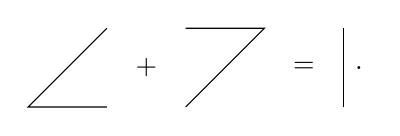
\begin{tikzpicture}
            \draw (1,1) -- (0,0)-- (1,0);
            \draw (1.5,0.5) node{$+$};
            \draw (2,1) -- (3,1) -- (2,0);
            \draw (3.5,0.5) node{$=$};
            \draw (4,1) -- (4,0);
            \draw (4.2,0.5) node {.};
          \end{tikzpicture}
      \]
    \item
      A family~$s = (s_n)_{n \in \Integer}$ of morphisms~$s_n \colon C_n \to D_{n+1}$ with~$f-g = ds + sd$, i.e.\ a null homotopy for~$f-g$, is a \emph{homotopy}\index{homotopy} between~$f$ and~$g$.
  \end{enumerate}
\end{remark*}


\begin{remark}
  Let~$\Ccc$ and~$\Dcc$ be morphisms of chain complexes in~$\Acat$.
  If~$(s_n)_{n \in \Natural}$ is any family of morphisms~$s_n \colon C_n \to D_{n+1}$ then~$f \defined (f_n)_{n \in \Integer}$ with~$f_n \defined d_{n+1} s_n + s_{n-1} d_n$ is a morphism of chain complexes~$f \colon \Ccc \to \Dcc$ because
  \[
      d{}f
    = d (ds + sd)
    = d^2 s + dsd
    = dsd
    = dsd + sd^2
    = (ds + sd) d
    = f d \,.
  \]
\end{remark}

\begin{lemma}
  Let~$\Ccc$ and~$\Dcc$ be chain complexes and let~$f, g \colon \Ccc \to \Dcc$ be two parallel morphisms.
  \begin{enumerate}
    \item
      \label{null homotopic is zero in homotopy}
      If the morphism~$f$ is null homotopic then~$\Hl_n(f) = 0$ for every~$n \in \Integer$.
    \item
      \label{homotopic morphisms are the same in homotopy}
      If the morphisms~$f$ and~$g$ are homotopic then~$\Hl_n(f) = \Hl_n(g)$ for every~$n \in \Integer$.
    \item
      If~$f$ is a homotopy equivalence then~$f$ is a {\qim}.
  \end{enumerate}
  The same holds for cochain complexes.
\end{lemma}


\begin{proof}
  \leavevmode
  \begin{enumerate}
    \item
      This is Exercise~1 of Exercise~sheet~9.
    \item
      This follows from part~\ref*{null homotopic is zero in homotopy} by the additivity of~$\Hl_n$.
    \item
      This follows from part~\ref*{homotopic morphisms are the same in homotopy} by the functoriality of~$\Hl_n$.
    \qedhere
  \end{enumerate}
\end{proof}


\begin{remark}
  At this point in the lecture it was remarked that the homology functors~$\Hl_n \colon \Ch(\Acat) \to \Acat$ are additive.
  We have (thanks to some personal modifications) already seen this (in a slightly different way than in the lecture) in~\cref{functoriality of homology}.
%   We have seen in~\cref{functoriality of homology} that the functors~$\Hl_n \colon \Ch(\Acat) \to \Acat$ with~$n \in \Integer$ are additive, but this can also seen as follows:
%   
%   For any two morphisms~$f_1 \colon X_1 \to Y_1$ and~$f'_2 \colon X_2 \to Y_2$ in~$\Acat$, then we get the combined morphism
%   \[
%             \begin{bmatrix}
%               f_1 &     \\
%                   & f_2
%             \end{bmatrix}
%     \colon  X_1 \oplus X_2
%     \to     Y_1 \oplus Y_2 \,.
%   \]
%   If~$k_1 \colon \ker(f_1) \to X_1$ is a kernel of~$f_1$ and~$k_2 \colon \ker(f_2) \to X_2$ is a kernel of~$f_2$, then
%   \[
%             \begin{bmatrix}
%               k_1 &     \\
%                   & k_2
%             \end{bmatrix}
%     \colon  \ker(f_1) \oplus \ker(f_2)
%     \to     X_1 \oplus X_2
%   \]
%   is a kernel of~$\begin{bsmallmatrix} f_1 & \\ & f_2 \end{bsmallmatrix}$.
%   Dually, if~$c_1 \colon Y_1 \to \coker(f_1)$ and~$c_2 \colon Y_2 \to \coker(f_2)$ are cokernels of~$f_1$ and~$f_2$ then
%    \[
%             \begin{bmatrix}
%               c_1 &     \\
%                   & c_2
%             \end{bmatrix}
%     \colon  Y_1 \oplus Y_2
%     \to     \coker(f_1) \oplus \coker(f_2)
%   \]
%   is a cokernel of~$\begin{bsmallmatrix} f_1 & \\ & f_2 \end{bsmallmatrix}$.
%   It also follows by combining both of these observations that if~$i_1 \colon \im(f_1) \to Y_1$ and~$i_2 \colon \im(f_2) \to Y_2$ are images of~$f_1$ and~$f_2$, then
%   \[
%             \begin{bmatrix}
%               i_1 &     \\
%                   & i_2
%             \end{bmatrix}
%     \colon  \im(f_1) \oplus \im(f_2)
%     \to     Y_1 \oplus Y_2
%   \]
%   is a cokernel of~$\begin{bsmallmatrix} f_1 & \\ & f_2 \end{bsmallmatrix}$.
%   
%   Let~$\Ccc^{(1)}$ and~$\Ccc^{(2)}$ be two chain complexes.
%   For~$j = 1, 2$ let
%   \[
%     p^{(j)}_n \colon C^{(j)}_{n-1} \to \Bl_n(\Ccc^{(j)})
%     \quad\text{and}\quad
%     i^{(j)}_n \colon \Zl_n(\Ccc^{(j)}) \to C^{(j)}_n
%   \]
%   be the canonical morphisms and let~$\lambda^{(j)} \colon \Bl_n(\Ccc^{(j)}) \to \Zl_n(\Ccc^{(j)})$ be the canonical morphism, i.e.\ the unique morphism that makes the following diagram commute:
%   \[
%     \begin{tikzcd}[column sep = tiny]
%         \dotsb
%         \arrow{rr}
%       & {}
%       & C^{(j)}_{n+1}
%         \arrow{rr}[above]{d^{(j)}_{n+1}}
%         \arrow{dr}
%       & {}
%       & C^{(j)}_n
%         \arrow{rr}[above]{d^{(j)}_n}
%       & {}
%       & C^{(j)}_{n-1}
%         \arrow{rr}
%       & {}
%       & \dotsb
%       \\
%         {}
%       & {}
%       & {}
%       & \Bl_n(\Ccc^{(j)})
%         \arrow{ur}
%         \arrow[dashed]{rr}
%       & {}
%       & \Zl_n(\Ccc^{(j)})
%         \arrow{ul}
%       & {}
%       & {}
%       & {}
%     \end{tikzcd}
%   \]
%   The differential~$d$ of~$\Ccc^{(1)} \oplus \Ccc^{(2)}$ is given by
%   \[
%       d_n
%     = \begin{bmatrix}
%         d^{(1)}_n &           \\
%                   & d^{(2)}_n
%       \end{bmatrix}
%   \]
%   for every~$n \in \Integer$.
%   It follows from the above observations that
%   \[
%       \Zl_n( \Ccc^{(1)} \oplus \Ccc^{(2)} )
%     = \Zl_n(\Ccc^{(1)}) \oplus \Zl_n(\Ccc^{(2)}) \,,,
%   \]
\end{remark}


\begin{example}
  Let~$f, g \colon X \to Y$ be two continuous maps between topological spaces~$X$ and~$Y$.
  If the maps~$f$ and~$g$ are homotopic then their induced morphisms of chain complexes~$f_*, g_* \colon \Ccc^\sing(X) \to \Ccc^\sing(Y)$ are again homotopic.
\end{example}


\begin{remarkdefinition}
  \label{definition of homotopy category}
  Let~$\Bcc$,~$\Ccc$,~$\Dcc$ and~$\Ecc$ be chain complexes in~$\Acat$.
  \begin{enumerate}
    \item
      The set
      \[
          N
        = \{
            f \in \Hom_{\Ch(\Acat)}(\Ccc, \Dcc)
          \suchthat
            \text{$f$ is null homotopic}
          \}
      \]
      is a subgroup of~$\Hom_{\Ch(\Acat)}(\Ccc, \Dcc)$:
      \begin{itemize}
        \item
          It holds that~$0 \in \Hom_{\Ch(\Acat)}(\Ccc, \Dcc)$, i.e.\ the zero morphism is null homotopic.
          This can be seen by choosing for the required nullhomotpy~$s = (s_n)_{n \in \Integer}$ the zero morphism~$s_n = 0$ for every~$n \in \Integer$.
        \item
          If two morphisms of chain complexes~$f, g \colon \Ccc \to \Dcc$ are null homotopic then there exist null homotopies~$s = (s_n)_{n \in \Integer}$ and~$t = (t_n)_{n \in \Integer}$ for~$f$ and~$g$.
          Then~$u = (u_n)_{n \in \Integer}$ with~$u_n \defined s_n - t_n$ is a null homotopy for~$f - g$ because
          \begin{align*}
                du + ud
             =  d(s - t) + (s - t)d
            &=  ds - dt + sd - td \\
            &=  ds + sd - (dt + td)
             =  f - g \,.
          \end{align*}
          This show that for all~$f, g \in N$ also~$f - g \in N$.
      \end{itemize}
      It follows that homotopy of morphisms of chain complexes is an equivalence relation on~$\Hom_{\Ch(\Acat)}(\Ccc, \Dcc)$.
    \item
      \label{welldefinedness of sum}
      If~$f, f', g, g' \colon \Ccc \to \Dcc$ are morphisms of chain complexes with both~$f \sim g$ and~$f' \sim g'$ then also~$f + g \sim f' + g'$:
      We find for~$N$ as above that it follows from~$f - f', g - g' \in N$ that also
      \[
            (f + g) - (f' + g')
        =   (f - f') + (g - g')
        \in N \,,
      \]
      because~$N$ is a subgroup of~$\Hom_{\Ch(\Acat)}(X,Y)$.
    \item
      Let~$f \colon \Ccc \to \Dcc$ be a morphism of chain complexes that is null homotopic, say via a null homotopy~$(s_n)_{n \in \Integer}$.
      Then for every morphism of chain complexes~$g \colon \Dcc \to \Ecc$ the composition~$gf$ is again null homotopic:
      The family~$t = (t_n)_{n \in \Integer}$ given by~$t_n \defined g_{n+1} s_n$ is a null homotopy for~$gf$ because
      \[
          gf
        = g(ds + sd)
        = gds + gsd
        = dgs + gsd
        = dt + td \,.
      \]
      We find similarly that for every morphism of chain complexes~$h \colon \Bcc \to \Ccc$ the composition~$fh$ is again null homotopic:
      The family~$u = (u_n)_{n \in \Integer}$ given by~$u_n \defined s_n h_n$ is a null homotopy for~$fh$ because
      \[
          fh
        = (ds + sd)h
        = dsh + sdh
        = dsh + shd
        = du + ud \,.
      \]
      It follows for all morphisms of chain complexes~$f, f' \colon \Ccc \to \Dcc$ and~$g, g' \colon \Dcc \to \Ecc$ with~$f \sim f'$ and~$g \sim g'$ that also~$gf \sim g'f'$.
      Indeed, the difference
      \[
          gf - g'f'
        = gf - gf' + gf' - g'f'
        = g(f - f') + (g - g')f'
      \]
      is nullhomotpic because both~$f-f'$ and~$g-g'$ are null homotopic.
    \item
      This shows that the composition of morphisms in~$\Ch(\Acat)$ descends to a composition of equivalence classes with respect to homotopy.
      We hence obtain a category~$\Homotopy(\Acat)$ with
      \begin{itemize}
        \item
          objects~$\Ob(\Homotopy(\Acat)) \defined \Ob(\Ch(\Acat))$,
        \item
          morphism sets
          \begin{align*}
                        \Homotopy(\Acat)(\Ccc, \Dcc)
            \defined&{} \Hom_{\Ch(\Acat)}(\Ccc,\Dcc)/{\sim} \\
                   =&{} \Hom_{\Ch(\Acat)}(\Ccc,\Dcc)/\text{homotopy}
          \end{align*}
          for every two chain complexes~$\Ccc$ and~$\Dcc$ in~$\Acat$,
        \item
          and composition of morphisms~$[f] \colon \Ccc \to \Dcc$ and~$[g] \colon \Dcc \to \Ecc$ given by
          \[
                      [g] \circ [f]
            \defined  [g \circ f] \,.
          \]
      \end{itemize}
      The category~$\Homotopy(\Acat)$ is the \emph{homotopy category}\index{homotopy!category} of~$\Acat$.
    \item
      The homotopy category~$\Homotopy(\Acat)$ is again additve:
      The preadditive structure of~$\Homotopy(\Acat)$ is inherited from the category~$\Ch(\Acat)$ via
      \[
                  [f] + [g]
        \defined  [f + g]
      \]
      for any two parallel morphisms~$[f], [g] \colon \Ccc \to \Dcc$ in~$\Homotopy(\Acat)$.
      Part~\ref{welldefinedness of sum} shows that this addition is {\welldef}, and that~$\Homotopy(\Acat)$ satisfies the axioms of a preadditive category follows from~$\Ch(\Acat)$ satisfying these axioms.
      
      If~$\Ccc^{(1)}, \dotsc, \Ccc^{(n)}$ are finitely many chain complexes in~$\Acat$, i.e.\ objects of the homotopy category~$\Homotopy(\Acat)$, then a biproduct of~$\Ccc^{(1)}, \dotsc, \Ccc^{(n)}$ in~$\Homotopy(\Acat)$ is given by~$(\Ccc, ([c_i])_{i=1}^n, ([p_i])_{i=1}^n)$ if~$(\Ccc, (c_i)_{i=1}^n, (p_i)_{i=1}^n)$ is a biproduct of~$\Ccc^{(1)}, \dotsc, \Ccc^{(n)}$ in~$\Ch(\Acat)$.
  \end{enumerate}
\end{remarkdefinition}


\begin{warningnonum}
  Even though~$\Acat$ and~$\Ch(\Acat)$ are abelian, the homotopy category~$\Homotopy(\Acat)$ will in general not be abelian again.
  (A counterexample can be found in Exercise~4 of Exercise~sheet~9, where is shown that~$\Homotopy(\Ab)$ is not abelian.)
\end{warningnonum}


\begin{remark*}
  We may reformulate \cref{definition of homotopy category} using the language introduced in \cref{quotient categories}:
  The null homotopic morphisms of chain complexes form an ideal~$\Ndeal$ in the additive category~$\Ch(\Acat)$, whose corresponding additive congruence relation~$\sim$ is given by homotopy of morphisms of chain complex.
  The homotopy category~$\Homotopy(\Acat)$ is precisely the quotient category~$\Ch(\Acat)/\Ndeal = \Ch(\Acat)/{\sim}$.
\end{remark*}





\section{Mapping Cones}


\begin{definition}
  \leavevmode
  \begin{enumerate}
    \item
      Let~$f \colon \Ccc \to \Dcc$ be a morphism of chain complexes.
      The \emph{mapping cone}\index{mapping cone}\index{cone} of~$f$ is the chain complex~$\cone(f)$ that is given by
      \begin{itemize}
        \item
          the components~$\cone(f)_n \defined C_{n-1} \oplus D_n$ for every~$n \in \Integer$, together with
        \item
          the differential
          \[
                      d^{\,\cone(f)}_n
            \defined  \begin{bmatrix}
                        -d^{\,C}_{n-1}  & 0     \\
                        -f_{n-1}    & d^D_n
                      \end{bmatrix}
            \colon    C_{n-1} \oplus D_n
            \to       C_{n-2} \oplus D_{n-1}
          \]
          for every~$n \in \Integer$.
      \end{itemize}
    \item
      Let~$f \colon \Cccc \to \Dccc$ be a morphism of cochain complexes.
      The \emph{mapping cone}\index{mapping cone}\index{cone} of~$f$ is the cochain complex~$\cone(f)$ that is given by
      \begin{itemize}
        \item
          the components~$\cone(f)^n \defined C^{n+1} \oplus D^n$ for every~$n \in \Integer$, together with
        \item
          the differential
          \[
                      d_{\cone(f)}^n
            \defined  \begin{bmatrix}
                        -d_C^{n+1}  & 0     \\
                        -f^{n+1}    & d_D^n
                      \end{bmatrix}
            \colon    C^{n+1} \oplus D^n
            \to       C^{n+2} \oplus D^{n+1}
          \]
          for every~$n \in \Integer$.
      \end{itemize}
  \end{enumerate}
\end{definition}


\begin{remark}
  If~$f \colon \Ccc \to \Dcc$ is a morphism of chain complexes, or~$f \colon \Cccc \to \Dccc$ a morphism of cochain complexes, then~$\cone(f)$ is indeed a (co)chain complex because
  \[
      \begin{bmatrix}
        -d  & 0 \\
        -f  & d \\
      \end{bmatrix}
      \begin{bmatrix}
        -d  & 0 \\
        -f  & d
      \end{bmatrix}
    = \begin{bmatrix}
        d^2    & 0   \\
        fd-df  & d^2
      \end{bmatrix}
    = \begin{bmatrix}
        0 & 0 \\
        0 & 0
      \end{bmatrix} \,.
  \]
\end{remark}


\begin{proposition}
  \label{exact sequence of cone}
  Let~$f \colon \Ccc \to \Dcc$ be a morphism of chain complexes.
  \begin{enumerate}
    \item
      The family~$\alpha = (\alpha_n)_{n \in \Integer}$ of morphisms
      \[
                  \alpha_n
        \defined  \begin{bmatrix}
                    0 \\
                    \id_{D_n}
                  \end{bmatrix}
        \colon    D_n
        \to       C_{n-1} \oplus D_n
      \]
      is a morphism of chain complexes~$\alpha \colon \Dcc \to \cone(f)$.
    \item
      The family~$\beta = (\beta_n)_{n \in \Integer}$ of morphisms
      \[
                  \beta_n
        \defined  \begin{bmatrix}
                    -\id_{C_{n-1}} & 0
                  \end{bmatrix}
        \colon    C_{n-1} \oplus D_n
        \to       C_{n-1}
      \]
      is a morphism of chain complexes~$\beta \colon \cone(f) \to \Ccc[-1]$.
    \item
      The morphisms~$\alpha$ and~$\beta$ fit into a short exact sequence
      \[
        0
        \to
        \Dcc
        \xlongto{\alpha}
        \cone(f)
        \xlongto{\beta}
        \Ccc[-1]
        \to
        0 \,.
      \]
    \item
      In the induced long exact homology sequence
      \[
        \begin{tikzcd}
            {}
          & \dotsb
            \arrow{r}
            \arrow[d, phantom, ""{coordinate, name=Y}]
          & \Hl_{n+1}(\Ccc[-1])
            \arrow[ dll,
                    "\del_{n+1}",
                    rounded corners,
                    to path={ -- ([xshift=2ex]\tikztostart.east)
                              |- (Y) \tikztonodes
                              -| ([xshift=-2ex]\tikztotarget.west)
                              -- (\tikztotarget)}
                  ]
          \\
            \Hl_n(\Dcc)
            \arrow{r}[above]{\Hl_n(\alpha)}
          & \Hl_n(\cone(f))
            \arrow{r}[above]{\Hl_n(\beta)}
            \arrow[d, phantom, ""{coordinate, name=Z}]
          & \Hl_n(\Ccc[-1])
            \arrow[ dll,
                    "\del_n",
                    rounded corners,
                    to path={ -- ([xshift=2ex]\tikztostart.east)
                              |- (Z) \tikztonodes
                              -| ([xshift=-2ex]\tikztotarget.west)
                              -- (\tikztotarget)}
                  ]
          \\
            \Hl_{n-1}(\Dcc)
            \arrow{r}
          & \dotsb
          & {}
        \end{tikzcd}
      \]
      the connecting morphism
      \[
        \del_{n+1}
        \colon
        \Hl_n(\Ccc)
        =
        \Hl_{n+1}(\Ccc[-1])
        \to
        \Hl_n(\Dcc)
      \]
      is given by~$\Hl_n(f)$ for every~$n \in \Integer$.
  \end{enumerate}
\end{proposition}


\begin{proof}
  This proof is currently missing from these notes, and will be added later.
  (The proof relies on the explicit construction of the connecting homomorphism in the \hyperref[snake lemma]{snake lemma}.)
% TODO: Add this proof.
\end{proof}


\begin{corollary}
  A morphism of chain complexes~$f \colon \Ccc \to \Dcc$ is a {\qim} if and only if its cone is acyclic.
\end{corollary}


\begin{proof}
  We get by~\cref{exact sequence of cone} a long exact sequence
  \[
    \dotsb
    \to
    \Hl_{n+1}(\cone(f))
    \to
    \Hl_n(\Ccc)
    \xlongto{\Hl_n(f)}
    \Hl_n(\Dcc)
    \to
    \Hl_n(\cone(f))
    \to
    \dotsb
  \]
  The morphism~$f$ is a {\qim} if and only if~$\Hl_n(f)$ is for every~$n \in \Integer$ an isomorphism.
  This holds by the exactness of the above sequence if and only if~$\Hl_n(\cone(f)) = 0$ for every~$n \in \Integer$.
  This is precisely what it means for~$\cone(f)$ to be acyclic.
\end{proof}





\lecturend{17}









\chapter{Derived Functors}





\section{Homological and Cohomological \texorpdfstring{$\delta$}{delta}-Functors}


\begin{conventionnonum}
  In the following,~$\Acat$ and~$\Bcat$ denote abelian categories.
\end{conventionnonum}


\begin{definition}[(Co)homological $\delta$-functors]
  \leavevmode
  \begin{enumerate}
    \item
      A \emph{homological~{\deltafun}}\index{homological-d-functor@homological $\delta$-functor}\index{d-functor@$\delta$-functor!homological} from~$\Acat$ to~$\Bcat$ is a pair~$((T_n)_{n \geq 0}, (\delta^\xi_n)_{n \geq 1, \xi})$ consisting of
      \begin{itemize}
        \item
          a family~$(T_n)_{n \geq 0}$ of additive functors~$T_n \colon \Acat \to \Bcat$, and
        \item
          a family~$(\delta^\xi_n)_{n \geq 1, \xi}$ of morphisms~$\delta^\xi_n \colon T_n(X'') \to T_{n-1}(X')$, where~$\xi$ ranges through the class of short exact sequences in~$\Acat$.
      \end{itemize}
      These data are subject to the following conditions:
      \begin{enumerate}[label=(H$\delta$\arabic*)]
        \item
          For every short exact sequence
          \[
            \xi
            \colon
            0
            \to
            X'
            \to
            X
            \to
            X''
            \to
            0
          \]
          in~$\Acat$, the resulting sequence
          \[
            \begin{tikzcd}[column sep = small]
                {}
              & \dotsb
                \arrow{r}
                \arrow[d, phantom, ""{coordinate, name=Z1}]
              & T_{n+1}(X'')
                \arrow[ dll,
                        "\delta^{\xi}_{n+1}",
                        rounded corners,
                        to path={ -- ([xshift=2ex]\tikztostart.east)
                                  |- (Z1) \tikztonodes
                                  -| ([xshift=-2ex]\tikztotarget.west)
                                  -- (\tikztotarget)}
                      ]
              & {}
              \\
                T_n(X')
                \arrow{r}
              & T_n(X)
                \arrow{r}
                \arrow[d, phantom, ""{coordinate, name=Z2}]
              & T_n(X'')
                \arrow[ dll,
                        "\delta^\xi_n",
                        rounded corners,
                        to path={ -- ([xshift=2ex]\tikztostart.east)
                                  |- (Z2) \tikztonodes
                                  -| ([xshift=-2ex]\tikztotarget.west)
                                  -- (\tikztotarget)}
                      ]
              & {}
              \\
                T_{n-1}(X')
                \arrow{r}
              & \dotsb
                \arrow{r}
                \arrow[d, phantom, ""{coordinate, name=Z3}]
              & T_1(X'')
                \arrow[ dll,
                        "\delta^\xi_1",
                        rounded corners,
                        to path={ -- ([xshift=2ex]\tikztostart.east)
                                  |- (Z3) \tikztonodes
                                  -| ([xshift=-2ex]\tikztotarget.west)
                                  -- (\tikztotarget)}
                      ]
              & {}
              \\
                T_0(X')
                \arrow{r}
              & T_0(X)
                \arrow{r}
              & T_0(X'')
                \arrow{r}
              & 0
            \end{tikzcd}
          \]
          in~$\Bcat$ is exact.
        \item
          If
          \[
            \begin{tikzcd}
                \xi:
                \quad
                0
                \arrow{r}
              & X'
                \arrow{r}
                \arrow[dashed]{d}[right]{f'}
              & X
                \arrow{r}
                \arrow[dashed]{d}[right]{f}
              & X''
                \arrow{r}
                \arrow[dashed]{d}[right]{f''}
              & 0
              \\
                \zeta:
                \quad
                0
                \arrow{r}
              & Y'
                \arrow{r}
              & Y
                \arrow{r}
              & Y''
                \arrow{r}
              & 0
            \end{tikzcd}
          \]
          is a commutative diagram in~$\Acat$ with (short) exact rows~$\xi$ and~$\zeta$, then the induced square
          \[
            \begin{tikzcd}
                T_n(X'')
                \arrow{r}[above]{\delta^\xi_n}
                \arrow[dashed]{d}[left]{T_n(f'')}
              & T_{n-1}(X')
                \arrow[dashed]{d}[right]{T_{n-1}(f')}
              \\
                T_n(Y'')
                \arrow{r}[above]{\delta^\zeta_n}
              & T_{n-1}(Y')
            \end{tikzcd}
          \]
          commutes for every~$n \geq 1$.
      \end{enumerate}
     \item
      A \emph{cohomological~{\deltafun}}\index{cohomological-d-functor@cohomological $\delta$-functor}\index{d-functor@$\delta$-functor!cohomological} from~$\Acat$ to~$\Bcat$ is a pair~$((T^n)_{n \geq 0}, (\delta_\xi^n)_{n \geq 0, \xi})$ consisting of
      \begin{itemize}
        \item
          a family~$(T^n)_{n \geq 0}$ of additive functors~$T^n \colon \Acat \to \Bcat$, and
        \item
          a family~$(\delta_\xi^n)_{n \geq 0, \xi}$ of morphisms~$\delta_\xi^n \colon T^n(X'') \to T^{n+1}(X')$, where~$\xi$ ranges through the class of short exact sequences in~$\Acat$.
      \end{itemize}
      These data are subject to the following conditions:
      \begin{enumerate}[label=(C$\delta$\arabic*)]
        \item
          For every short exact sequence
          \[
            \xi
            \colon
            0
            \to
            X'
            \to
            X
            \to
            X''
            \to
            0
          \]
          in~$\Acat$, the resulting sequence
          \[
            \begin{tikzcd}[column sep = small]
                0
                \arrow{r}
              & T^0(X')
                \arrow{r}
                \arrow[d, phantom, ""{coordinate, name=Z1}]
              & T^0(X)
                \arrow{r}
              & T^0(X'')
                \arrow[ dll,
                        "\delta_{\xi}^0",
                        rounded corners,
                        to path={ -- ([xshift=2ex]\tikztostart.east)
                                  |- (Z1) \tikztonodes
                                  -| ([xshift=-2ex]\tikztotarget.west)
                                  -- (\tikztotarget)}
                      ]
              \\
                {}
              & T^1(X')
                \arrow{r}
              & \dotsb
                \arrow{r}
                \arrow[d, phantom, ""{coordinate, name=Z2}]
              & T^n(X'')
                \arrow[ dll,
                        "\delta_\xi^n",
                        rounded corners,
                        to path={ -- ([xshift=2ex]\tikztostart.east)
                                  |- (Z2) \tikztonodes
                                  -| ([xshift=-2ex]\tikztotarget.west)
                                  -- (\tikztotarget)}
                      ]
              \\
                {}
              & T^{n+1}(X')
                \arrow{r}
              & T^{n+1}(X)
                \arrow{r}
                \arrow[d, phantom, ""{coordinate, name=Z3}]
              & T^{n+1}(X'')
                \arrow[ dll,
                        "\delta_\xi^{n+1}",
                        rounded corners,
                        to path={ -- ([xshift=2ex]\tikztostart.east)
                                  |- (Z3) \tikztonodes
                                  -| ([xshift=-2ex]\tikztotarget.west)
                                  -- (\tikztotarget)}
                      ]
              \\
                {}
              & T^{n+2}(X')
                \arrow{r}
              & \dotsb
              & {}
            \end{tikzcd}
          \]
          in~$\Bcat$ is exact.
        \item
          If
          \[
            \begin{tikzcd}
                \xi:
                \quad
                0
                \arrow{r}
              & X'
                \arrow{r}
                \arrow[dashed]{d}[right]{f'}
              & X
                \arrow{r}
                \arrow[dashed]{d}[right]{f}
              & X''
                \arrow{r}
                \arrow[dashed]{d}[right]{f''}
              & 0
              \\
                \zeta:
                \quad
                0
                \arrow{r}
              & Y'
                \arrow{r}
              & Y
                \arrow{r}
              & Y''
                \arrow{r}
              & 0
            \end{tikzcd}
          \]
          is a commutative diagram in~$\Acat$ with (short) exact rows~$\xi$ and~$\zeta$, then the induced square
          \[
            \begin{tikzcd}
                T^n(X'')
                \arrow{r}[above]{\delta_\xi^n}
                \arrow[dashed]{d}[left]{T^n(f'')}
              & T^{n+1}(X')
                \arrow[dashed]{d}[right]{T^{n+1}(f')}
              \\
                T^n(Y'')
                \arrow{r}[above]{\delta_\zeta^n}
              & T^{n+1}(Y')
            \end{tikzcd}
          \]
          commutes for every~$n \geq 0$.
      \end{enumerate}
  \end{enumerate}
\end{definition}


\begin{remark}
  \leavevmode
  \begin{enumerate}
    \item
      If~$\Tdeltah = ((T_n)_{n \geq 0}, (\delta_n^\xi)_{n \geq 0, \xi})$ is a homological~{\deltafun} from~$\Acat$ to~$\Bcat$ then we get a cohomological~{\deltafun}~$\Tdeltac = ((T^n)_{n \geq 0}, (\delta_\xi^n)_{n \geq 0, \xi})$ from~$\Acat^\op$ to~$\Bcat^\op$ by setting
      \[
                  T^n
        \defined  T_n
        \colon    \Acat
        \to       \Bcat
      \]
      for every~$n \in \Integer$, and
      \[
                \delta_\xi^n
        =       \delta^\xi_{n+1}
        \colon  T^n(X'')
        \to     T^{n+1}(X')
      \]
      for all~$n \geq 0$ and every short exact sequence
      \[
        \xi
        \colon
        0
        \to
        X'
        \to
        X
        \to
        X''
        \to
        0
      \]
      in~$\Acat^\op$.
      (Note that the above short exact sequence in~$\Acat^\op$ is the same as a short exact sequence
      \[
        0
        \from
        X'
        \from
        X
        \from
        X''
        \from
        0
        \cocolon
        \xi
      \]
      in~$\Acat$, and that the resulting connecting morphism~$\delta^\xi_{n+1} \colon T_{n+1}(X') \to T_n(X'')$ in~$\Bcat$ is a morphism~$T^n(X'') \to T^{n+1}(X')$ in~$\Bcat^\op$.)
      The converse construction also works, and hence homological~{\deltafuns}~$\Acat \to \Bcat$ are the same as cohomological~{\deltafuns}~$\Acat^\op \to \Bcat^\op$.
    \item
      If~$\Tdeltah$ is a homological~{\deltafun} then its zeroth component~$T_0$ is right exact.
    \item
      If~$\Tdeltac$ is a cohomological~{\deltafun} then its zeroth component~$T^0$ is left exact.
  \end{enumerate}
\end{remark}


\begin{example}
  Let~$\Chh_{\geq 0}(\Acat)$ be the full subcategories of~$\Ch(\Acat)$ whose objects are given by those chain complexes~$\Ccc$ in~$\Acat$ with~$C_n = 0$ for every~$n < 0$.
  This subcategory of~$\Ch(\Acat)$ is closed under taking biproducts, kernels and cokernels.
  Hence~$\Ch(\Acat)$ is again abelian (and the inclusion functor~$\Chh_{\geq 0}(\Acat) \to \Ch(\Acat)$ is exact).
  The long exact sequence of homology, together with the connecting morphisms~$\del^\xi_n$, result in a~{\deltafun}~$\Hldeltah = ((\Hl_n)_{n \geq 0}, (\del^\xi_n)_{n \geq 1, \xi})$ from~$\Chh_{\geq 0}(\Acat)$ to~$\Acat$.
  
  Dually, the full subcategory~$\CChh^{\geq 0}(\Acat)$ of~$\CCh(\Acat)$, whose objects are given by those cochain complexes~$\Cccc$ in~$\Acat$ with~$C^n = 0$ for every~$n < 0$, is again abelian, and~$\Hldeltac = ((\Hl^n)_{n \geq 0}, (\del_\xi^n)_{n \geq 0})$ is a~{\deltafun} from~$\CChh_{\geq 0}(\Acat)$ to~$\Acat$.
\end{example}


\begin{example}
  Let~$A$ be a~{\kalg} and let~$a \in A$.
  The~\emph{\dash{$a$}{torsion}}\index{torsion} of an~{\module{$A$}}~$M$ is
  \[
              {}_{(a)} M
    \defined  \{
                m \in M
              \suchthat
                am = 0
              \} \,,
  \]
  which is a~{\submodule{$\kf$}} of~$M$.
  For every short exact sequence of~{\modules{$A$}}
  \[
    0
    \to
    M'
    \to
    M
    \to
    M''
    \to
    0
  \]
  we get the following commutative diagram of~{\modules{$\kf$}} with (short) exact rows:
  \[
    \begin{tikzcd}
        0
        \arrow{r}
      & M'
        \arrow{r}
        \arrow[dashed]{d}[right]{a \cdot (-)}
      & M
        \arrow{r}
        \arrow[dashed]{d}[right]{a \cdot (-)}
      & M''
        \arrow{r}
        \arrow[dashed]{d}[right]{a \cdot (-)}
      & 0
      \\
        0
        \arrow{r}
      & M'
        \arrow{r}
      & M
        \arrow{r}
      & M''
        \arrow{r}
      & 0
    \end{tikzcd}
  \]
  It follows from the snake lemma that we get a long exact sequence of~{\modules{$\kf$}}
  \[
    0
    \to
    {}_{(a)} M'
    \to
    {}_{(a)} M
    \to
    {}_{(a)} M''
    \xlongto{\delta}
    M'/aM'
    \to
    M/aM
    \to
    M''/aM''
    \to
    0 \,.
  \]
  For the additive functors~$T^n \colon \Modl{A} \to \Modl{\kf}$ with
  \[
              T^0(M)
    \defined  {}_{(a)} M
    \quad\text{and}\quad
              T^1(M)
    \defined  M/aM
  \]
  for every~{\module{$A$}}~$M$, and~$T^n = 0$ for every~$n \geq 2$, we get from the above a cohomological~{\deltafun}~$\Tdeltac \colon \Modl{A} \to \Modl{\kf}$.
\end{example}


\begin{definition}
  \leavevmode
  \begin{enumerate}
    \item
      Let~$\Sdeltah, \Tdeltah \colon \Acat \to \Bcat$ be two parallel homological~{\deltafuns}.
      A \emph{morphism}\index{morphism!of!homological d-functors@homological $\delta$-functors} of homological~{\deltafun}~$\eta \colon \Sdeltah \to \Tdeltah$ is a family~$\eta = (\eta_n)_{n \geq 0}$ of natural transformations~$\eta_n \colon S_n \to T_n$ such that for every short exact sequence
      \[
        \xi
        \colon
        0
        \to
        X'
        \to
        X
        \to
        X''
        \to
        0
      \]
      in~$\Acat$ the induced square
      \[
        \begin{tikzcd}
            T_n(X'')
            \arrow{r}[above]{\delta^\xi_n}
            \arrow[dashed]{d}[left]{(\eta_n)_{X''}}
          & T_{n-1}(X')
            \arrow[dashed]{d}[right]{(\eta_{n-1})_{X'}}
          \\
            S_n(X'')
            \arrow{r}[above]{\delta^\xi_n}
          & S_{n-1}(X'')
        \end{tikzcd}
      \]
      in~$\Bcat$ commutes for every~$n \geq 1$.
    \item
      Let~$\Sdeltac, \Tdeltac \colon \Acat \to \Bcat$ be two parallel cohomological~{\deltafuns}.
      A \emph{morphism}\index{morphism!of!cohomological d-functors@cohomological $\delta$-functors} of cohomological~{\deltafun}~$\eta \colon \Sdeltac \to \Tdeltac$ is a family~$\eta = (\eta^n)_{n \geq 0}$ of natural transformations~$\eta^n \colon S^n \to T^n$ such that for every short exact sequence
      \[
        \xi
        \colon
        0
        \to
        X'
        \to
        X
        \to
        X''
        \to
        0
      \]
      in~$\Acat$ the induced square
      \[
        \begin{tikzcd}
            T^n(X'')
            \arrow{r}[above]{\delta_\xi^n}
            \arrow[dashed]{d}[left]{\eta^n_{X''}}
          & T^{n+1}(X')
            \arrow[dashed]{d}[right]{\eta^{n+1}_{X'}}
          \\
            S^n(X'')
            \arrow{r}[above]{\delta_\xi^n}
          & S^{n+1}(X'')
        \end{tikzcd}
      \]
      in~$\Bcat$ commutes for every~$n \geq 0$.
    \item
      A homological~{\deltafun}~$\Udeltah \colon \Acat \to \Bcat$ is \emph{universal}\index{universal d-functor@universal $\delta$-functor}\index{homological d-functor@homological $\delta$-functor!universal} if for every homological~{\deltafun}~$\Tdeltah \colon \Acat \to \Bcat$, every natural transformation~$\eta_0 \colon T_0 \to U_0$ can be uniquely extended to a morphism of homological~{\deltafuns}~$\eta \colon \Tdeltah \to \Udeltah$.
    \item
      A cohomological~{\deltafun}~$\Udeltac \colon \Acat \to \Bcat$ is \emph{universal}\index{universal d-functor@universal $\delta$-functor}\index{cohomological d-functor@cohomological $\delta$-functor!universal} if for every cohomological~{\deltafun}~$\Tdeltac \colon \Acat \to \Bcat$, every natural transformation~$\eta^0 \colon U^0 \to T^0$ can be extended uniquely to a morphism of cohomological~{\deltafuns}~$\eta \colon \Udeltac \to \Tdeltac$.
  \end{enumerate}
\end{definition}





\lecturend{18}





\chapter{Projectives and Injectives in Interesting Categories}
\chaptermark{Proj.\ and Inj.\ in Int.\ Cat.}




\section{Projectives in Module Categories}



\begin{conventionnonum}
  Let~$\kf$ be a commutative ring and let~$A$ be a~{\kalg}.
\end{conventionnonum}


\begin{lemma}
  \label{projective iff summand of free}
  A left~{\module{$A$}}~$P$ is projective if and only if it is a direct summand of a free~{\module{$A$}}.
\end{lemma}


\begin{proof}
  This is Exercise~4 on Exercise~sheet~10.
\end{proof}


\begin{corollary}
  The module category~$\Modl{A}$ has enough projectives.
\end{corollary}


\begin{proof}
  If~$M$ is any~{\module{$A$}} with generating set~$\{x_i\}_{i \in I}$ then there exists a surjective homomorphism of~{\modules{$A$}}~$A^{\oplus I} \to M$, with~$A^{\oplus I}$ being free and hence projective by \cref{projective iff summand of free}
\end{proof}


\begin{remark}
  \Cref{projective iff summand of free} also holds for right modules, whence~$\Modr{A}$ has enough projectives as well.
\end{remark}


\begin{remark}
  Let~$\indmodule{M}[A]$ and~$\indmodule[A]{N}$ be~{\modules{$A$}}.
  \begin{enumerate}
    \item
      The functors
      \begin{align*}
        - \tensor_A N
        \colon
        \Modr{A}
        \to
        \Modl{\kf}
        \quad&\text{and}\quad
        M \tensor_A -
        \colon
        \Modl{A}
        \to
        \Modl{\kf}
      \intertext{are right exact and hence admit left derived functors}
        \Leftdelta(- \tensor_A N)
        \colon
        \Modr{A}
        \to
        \Modl{k}
        \quad&\text{and}\quad
        \Leftdelta(M \tensor_A -)
        \colon
        \Modl{A}
        \to
        \Modl{\kf}  \,.
      \end{align*}
    \item
      The category~$(\Modl{A})^\op$ has enough injectives because the category~$\Modl{A}$ has enough projectives.
      The functor
      \[
        \Hom_A(-,N)
        \colon
        (\Modl{A})^\op
        \to
        \Modl{\kf}
      \]
      is left exact and does therefore admit a right derived functor
      \[
        \Rightdelta \Hom_A(-,N)
        \colon
        (\Modl{A})^\op
        \to
        \Modl{\kf}  \,.
      \]
  \end{enumerate}
\end{remark}


\begin{remark}
  Let~$A$ be a left noetherian~{\kalg}.
  Then the category~$\Modlfg{A}$ of finitely generated left~{\modules{$A$}} is abelian and the forgetful functor
  \[
    U
    \colon
    \Modlfg{A}
    \to
    \Modl{A}
  \]
  is exact.
  The exact functor~$U$ is in particular right exact and hence respects cokernels.
  Therefore a morphism in~$\Modlfg{A}$ is an epimorphism if and only if it is an epimorphism in~$\Modl{A}$.
  It follows that an object~$P$ of~$\Modlfg{A}$ is projective if and only if it is a direct summand of a finitely 
  generated free~{\module{$A$}}.
  
  For finitely generated~{\module{$A$}}~$\indmodule{M}[A]$ and~$\indmodule[A]{N}$ the functors
  \[
    - \tensor_A N
    \colon
    \Modlfg{A}
    \to
    \Modl{\kf}
    \quad\text{and}\quad
    M \tensor_A -
    \colon
    \Modlfg{A}
    \to
    \Modl{\kf}
  \]
  are right exact, and the functor
  \[
    \Hom_A(-,N)
    \colon
    (\Modlfg{A})^\op
    \to
    \Modl{\kf}
  \]
  is left exact.
  It follows from the exactness of the forgetful functor~$U$ by~\cref{exact functors respect derived} that their right, resp.\ left derived functor agrees with the right, resp.\ left derived functor for~$\Modl{A}$, resp.~$(\Modl{A}^\op)$.
\end{remark}








\section{Projectives in the Category of Quiver Representations}


\begin{conventionnonum}
  Let~$\kf$ be a field,~$Q$ a finite quiver (i.e.~$Q_0$ is finite), and abbreviate~$A \defined \kf Q$.
\end{conventionnonum}


\begin{definition}
  \leavevmode
  \begin{enumerate}
    \item
      For all vertices~$i, j \in Q_0$ let
      \[
        Q_*(i,j)
        =
        \{
          p \in Q_*
        \suchthat
          s(p) = i,
          t(p) = j
        \}
      \]
      be the set of paths from~$i$ to~$j$ in~$Q$.
    \item
      For every vertex~$i \in Q_0$ let~$P(i)$ be the representation of~$Q$ over~$\kf$ that is given by the following data:
      \begin{itemize}
        \item
          For every vertex~$j \in Q_0$ the~{\kvs}~$P(i)_j$ is the free~{\kvs} with basis~$Q(i,j)$.
        \item
          For every arrow~$\alpha \in Q_1$ with~$\alpha \colon j \to k$ the~{\klin} map~$P(i)_\alpha \colon P(i)_j \to P(i)_k$ is given on the basis~$Q(i,j)$ of~$P(i)_j$ by the concatenation of paths.
          We hence have for every~$p \in Q(i,j)$ that
          \[
            P(i)_\alpha(p)
            =
            \alpha \circ p  \,.
          \]
      \end{itemize}
  \end{enumerate}
\end{definition}


\begin{remark}
  Recall the equivalence of categories~$F \colon \Rep{\kf}{Q} \to \Modl{A}$ from part~\ref*{quiver reps are modules over path algebra} of \cref{examples for equivalences}:
  For every representation~$X$ of~$Q$ over~$\kf$ the~{\module{$A$}}~$M \defined F(X)$ has the underlying~{\kvs}
  \[
    M
    =
    \bigoplus_{j \in Q_0} X_j  \,,
  \]
  and the action of an arrow~$\alpha \colon j \to k$ (i.e.\ an element of the basis~$Q_*$ of~$A$) on~$M$ is given by the composition
  \[
    M
    \xlongto{\text{projection}}
    X_j
    \xlongto{X_\alpha}
    X_k
    \xlongto{\text{inclusion}}
    M \,.
  \]
  Under this equivalence of categories the representation~$P(i)$ corresponds to
  \[
    F(P(i))
    \cong
    A \varepsilon_i \,.
  \]
  
  Indeed, the~{\kvs}~$F(P(i)) = \bigoplus_{j \in Q_0} P(i)_j$ has as a basis the set of paths
  \begin{equation}
  \label{paths starting in i}
    \{
      p \in Q_*
    \suchthat
      s(p) = i
    \}  \,.
  \end{equation}
  This is also a basis of~$A \varepsilon_i$:
  We have for every~$p \in Q_*$ that
  \[
    p \varepsilon_i
    =
    \begin{cases}
      p & \text{if~$s(p) = i$}  \,, \\
      0 & \text{otherwise}  \,,
    \end{cases}
  \]
  and hence find that the linearly independent set~\eqref{paths starting in i} is a generating set, and therefore basis, for~$A \varepsilon_i$.
  The action of an arrow~$\alpha \in Q_1$ on a basis element~$p$ from~\eqref{paths starting in i} is for~$\alpha \colon j \to k$ given by
  \[
    \alpha p
    =
    \begin{cases}
      \alpha \circ p  & \text{if~$t(\alpha) = s(p)$}  \,, \\
      0               & \text{otherwise}  \,,
    \end{cases}
    =
    \begin{cases}
      \alpha \circ p  & \text{if~$s(p) = j$}  \,, \\
      0               & \text{otherwise}  \,,
    \end{cases}
    =
    P(i)_\alpha(p)  \,.
  \]
  This shows that the actions of~$A$ on~$M$ and~$A \varepsilon_i$ coincide.
\end{remark}


\begin{corollary}
  The representations~$P(i)$ of~$Q$ are projective objects of~$\Rep{\kf}{Q}$.
\end{corollary}


\begin{proof}
  It sufficies to show that the~{\modules{$A$}}~$A \varepsilon_i$ are projective.
  We observe that
  \begin{align*}
    A
    &=
    \bigoplus_{i \in Q_0}
    A \varepsilon_i
  \shortintertext{because on the level of bases}
    Q_*
    &=
    \coprod_{i \in Q_0}
    \{
      p \in Q_*
    \suchthat
      s(p) = i
    \}  \,.
  \end{align*}
  The~$A \varepsilon_i$ are therefore direct summands of the free~{\module{$A$}}~$A$, whence projective.
\end{proof}


\begin{lemma*}
  \label{homomorphisms out of P(i)}
  For every representation~$X$ of~$Q$ over~$\kf$ the map
  \[
    \Hom(P(i), X)
    \to
    X_i \,,
    \quad
    f
    \mapsto
    f_i(\varepsilon_i)
  \]
  is an isomorphism of~{\kvs}.
\end{lemma*}


\begin{proof}
  This is part~(i) of Exercise~4 of Exercise sheet~11.
\end{proof}


\begin{definition*}
  A quiver~$Q$ is \emph{acyclic}\index{acyclic!quiver}\index{quiver!acyclic} if it contains no oriented circles (of length~$\geq 1$).
\end{definition*}


\begin{corollary*}
  If the quiver~$Q$ is acyclic then every~$P(i)$ is~{\fd} with~$\End_k(P(i)) = k$.
\end{corollary*}


\begin{proof}
  This is part~(iii) of Exercise~4 of Exercise sheet~11.
\end{proof}


\begin{remark}
  If the quiver~$Q$ is acyclic then~$A$ is~{\fd} and every~$P(i)$ is indecomposable.
  (This is part~(iv) of Exercise~4 of Exercise sheet~11.)
\end{remark}


\begin{theoremnonum}[Krull--Remak--Schmidt]
  Let~$X$ be a~{\fd} representation of an acyclic quiver~$Q$.
  \begin{enumerate}
    \item
      There exists a decomposition~$X \cong X_1^{\oplus a_1} \oplus \dotsb \oplus X_r^{\oplus a_r}$ with~$X_i$ indecomposable,~$X_i \ncong X_j$ for~$i \neq j$ and~$a_i > 0$ for every~$i$.
    \item
      If~$X \cong Y_1^{\oplus b_1} \oplus \dotsb \oplus Y_s^{\oplus b_s}$ is another such decomposition then~$r = s$ and, up to reordering,~$X_i \cong Y_i$ and~$a_i = b_i$ for every~$i$.
  \end{enumerate}
\end{theoremnonum}


\begin{remarknonum}
  We will not prove the Krull--Remak--Schmidt theorem.
  A proof can be found in \cite{Elements}.
% TODO: Make this reference more specific.
\end{remarknonum}


\begin{remark*}
  The Krull--Remak--Schmidt theorem holds for every~{\kalg}~$A$ and every {\fd}~{\module{$A$}}~$M$;
  it holds even more generally for every ring~$R$ and every~{\module{$R$}}~$M$ of finite length.
  We will use the Krull--Remak--Schmidt theorem to show that every~{\fd} projective representation of~$Q$ over~$\kf$ is isomorphic to a direct sum of copies of~$P(i)$.
% TODO: When do we show this?
\end{remark*}


\begin{theorem}[The standard projective resolution]
  Let~$M$ be a~{\module{$A$}}.%
  \footnote{We do not require~$M$ to be~{\fd}, nor~$Q$ to be acyclic.}
  Then the sequence
  \[
    0
    \to
    \bigoplus_{\alpha \in Q_1}
    A \varepsilon_{t(\alpha)} \tensor_\kf \varepsilon_{s(\alpha)} M
    \xlongto{f}
    \bigoplus_{i \in Q_0}
    A \varepsilon_i \tensor_\kf \varepsilon_i M
    \xlongto{g}
    M
    \to
    0
  \]
  given by the~{\klin}~maps
  \begin{align*}
    g( (a_i \tensor x_i)_i )
    &\defined
    \sum_{i \in Q_0} a_i x_i
  \shortintertext{and}
    f( (a_\alpha \tensor x_\alpha)_\alpha )
    &\defined
    \sum_{\alpha \in Q_1}
    \Bigl(
      \iota_{s(\alpha)}( a_\alpha \alpha \tensor x_\alpha )
    - \iota_{t(\alpha)}( a_\alpha \tensor \alpha x_\alpha )
    \Bigr)
  \end{align*}
  is exact, and the appearing~{\modules{$A$}}
  \[
    P_0
    \defined
    \bigoplus_{i \in Q_0} A \varepsilon_i \tensor_\kf \varepsilon_i M
    \qquad\text{and}\qquad
    P_1
    \defined
    \bigoplus_{\alpha \in Q_1} A \varepsilon_{t(\alpha)} \tensor_\kf \varepsilon_{s(\alpha)} M
  \]
  are projective.
\end{theorem}


\begin{proof}
  The~{\klin} maps~$f$ and~$g$ are {\welldef}, and~$f \circ g = 0$.
  We have for every~$m \in M$ that
  \[
    m
    =
    1 \cdot m
    =
    \sum_{i \in Q_0} \varepsilon_i m
    =
    \sum_{i \in Q_0} \varepsilon_i^2 m
    =
    g\left( \sum_{i \in Q_0} \varepsilon_i \otimes \varepsilon_i m \right)
  \]
  which shows that~$g$ is surjective.
  The~{\modules{$A$}}~$P_0$ and~$P_1$ are projective because
  \[
    P_0
    \cong
    \bigoplus_{i \in Q_0}
    (A \varepsilon_i)^{\oplus \dim \varepsilon_i M}
    \quad\text{and}\quad
    P_1
    \cong
    \bigoplus_{\alpha \in Q_1}
    (A \varepsilon_{t(\alpha)})^{\oplus \dim \varepsilon_{s(\alpha)} M}
  \]
  are direct sums of the~{\modules{$A$}}~$A \varepsilon_i$.
  
  To show the injectivity of~$f$ and the exactness at~$P_0$ we observe that every element~$\xi \in P_0$ can be uniquely written as
  \[
    \xi
    =
    \left(
      \sum_{\substack{p \in Q_* \\ s(p) = i}}
      p \tensor \xi_p
    \right)_{i \in Q_0}
  \]
  with~$\xi_p \in \varepsilon_i A$ for~$i = s(p)$, because the set~$\{ p \in Q_* \suchthat s(p) = i \}$ is a basis for~$A \varepsilon_i$.
  The \emph{degree} of~$\xi \neq 0$ is given by
  \[
      \deg(\xi)
    = \max
      \{
        \ell(p)
      \suchthat
        \xi_p \neq 0
      \}  \,.
  \]
  
  \begin{claimnonum}
    For every~$\xi \in P_0$ the residue class~$\xi + \im(f)$ contains either~$0$ or an element of length~$0$.
  \end{claimnonum}
  
  \begin{proof}
    Suppose that~$\xi_p \neq 0$ for a path~$p \in Q_*$ with starting vertex~$i \defined s(p)$ such that~$\ell(p) \geq 1$.
    If~$\alpha$ denotes the starting arrow of~$p$ then there exists a unique path~$p' \in Q_*$ with~$p = p' \alpha$.
    We find for~$\zeta \in P_1$ with components~$\zeta_\alpha = p' \tensor \xi_p$ and~$\zeta_{\alpha'} = 0$ otherwise, i.e.
    \[
      ( \delta_{\alpha, \alpha'} p' \tensor \xi_p )_{\alpha' \in Q_1}
    \]
    that
    \[
      f( \zeta )
      =
        \iota_{s(\alpha)}(p' \alpha \tensor \zeta_p)
      - \iota_{t(\alpha)}(p' \tensor \alpha \zeta_p)
      =
        \iota_{s(\alpha)}(p \tensor \zeta_p)
      - \iota_{t(\alpha)}(p' \tensor \alpha \zeta_p)
    \]
    We have that~$s(\alpha) = s(p) = i$ because the path~$p$ starts with~$\alpha$.
    We hence find that the element
    \[
      \xi'
      \defined
      \xi - f(\zeta)
    \]
    differs from~$\xi$ in (at most) two coordinates:
    In the~\dash{$i$}{th} coordinate we’re losing the summand~$p \tensor \zeta_p$, while gaining the summand~$p' \tensor \alpha \zeta_p$ in the~\dash{$s(p')$}{th} coordinate.
    We note that both~$\xi'$ and~$\xi$ have the same residue class modulo~$\im(f)$, and that~$\ell(p') < \ell(p)$.
    
    We have thus shows that by changing the representative of the residue class~$\xi + \im(f)$ from~$\xi$ to~$\xi'$ we can replace a summand of length~$d$ in one coordinate by a summand of smaller length in another coordinate.
    By repeating this process finitely many times we arrive at a representative of the residue class~$\xi + \im(f)$ that is either of length~$0$ or just~$0$ itself.
%     We find for the element~$\zeta \in P_1$ given by
%     \[
%       \zeta
%       \defined
%       \left(
%         \sum_{\subalign{p &\in Q_* \\ \ell(p) &= d \\ p &= q \alpha}}
%         q \tensor \xi_p
%       \right)_{\alpha \in Q_1}
%     \]
%     that
%     \[
%       f(\zeta)
%       =
%       \sum_{\alpha \in Q_1}
%       \left(
%         \iota_{s(\alpha)}
%         \left(
%           \sum_{\subalign{p &\in Q_* \\ \ell(p) &= d}}
%             p \tensor \xi_p
%         \right)
%         -
%         \iota_{t(\alpha)}
%         \left(
%           \sum_{\subalign{p &\in Q_* \\ \ell(p) &= d \\ p &= q \alpha}}
%             q \tensor \alpha \xi_p
%         \right)
%       \right)
%     \]
%     It follows for the element~$\xi' \in P_0$ that
%     \[
%       \xi'
%       \defined
%       \xi- f(\zeta) \,.
%     \]
%     The elements~$\xi$ and~$\xi'$ have the same residue class module~$\im(f)$.
%     All paths of length~$d$ for~$\xi$ are canceled by~$f(\zeta)$, whence~$\deg(\xi') < d$.
%     The claim follows by induction hypothesis.
  \end{proof}
  
  We now show that~$\ker(g) \subseteq \im(f)$:
  Suppose that there exists some~$\xi \in \ker(g)$ with~$\xi \notin \im(f)$.
  Then the residue class~$\xi + \im(f)$ does not contain~$0$, and so we may assume by the above claim that~$\ell(\xi) = 0$.
  Then
  \[
    \xi
    =
    (
      \varepsilon_i \tensor \xi_{\varepsilon_i}
    )_{i \in Q_0}
  \]
  with~$\xi_{\varepsilon_i} \in \varepsilon_i M$ for every~$i \in Q_0$.
  We have that
  \[
    0
    =
    g(\xi)
    =
    \sum_{i \in Q_0}
    \varepsilon_i \xi_{\varepsilon_i}
    =
    \sum_{i \in Q_0}
    \xi_{\varepsilon_i}
  \]
  because it follows from~$\xi_{\varepsilon_i} \in \varepsilon_i M$ that~$\varepsilon_i \xi_{\varepsilon_i} = \xi_{\varepsilon_i}$.
  We find from the directness of the sum~$M = \bigoplus_{i \in Q_0} \varepsilon_i M$ that~$\xi_{\varepsilon_i} = 0$ for every~$i \in Q_0$, and hence~$\xi = 0$.
  But this contradicts~$\xi \notin \im(f)$.
  We find that indeed~$\ker(g) \subseteq \im(f)$.
  
  All that is left to show is the injectivity of~$f$:
  We may write~$\eta \in P_1$ uniquely as
  \[
    \eta
    =
    \left(
      \sum_{\substack{p \in Q_* \\ s(p) = t(\alpha)}}
      p \tensor \eta_{\alpha,p}
    \right)_{\alpha \in Q_1}
  \]
  with~$\eta_{\alpha, p} \in \varepsilon_{s(\alpha)} A$ for every~$\alpha \in Q_1$ and path~$p \in Q_*$ with~$s(p) = t(\alpha)$.
  Suppose that~$\eta \neq 0$.
  Let~$p_0 \in Q_*$ for which there exists an arrow~$\alpha \in Q_1$ with~$\eta_{p_0, \alpha} \neq 0$, and suppose that~$p_0$ is of maximal length with this property.
 We may write the element
  \[
    \xi
    \defined
    f(\eta)
    =
    \sum_{\alpha \in Q_1}
    \left(
      \iota_{s(\alpha)}
      \left(
        \sum_{\substack{p \in Q_* \\ s(p) = t(\alpha)}}
        p \alpha \tensor \eta_{\alpha,p}
      \right)
      -
      \iota_{t(\alpha)}
      \left(
        \sum_{\substack{p \in Q_* \\ s(p) = t(\alpha)}}
        p \tensor \alpha \eta_{\alpha,p}
      \right)
    \right)
  \]
  as
  \[
    \xi
    =
    \left(
      \sum_{\substack{p \in Q_* \\ s(p) = i}}
      p \tensor \xi_p
    \right)_{i \in Q_0}
  \]
  in the same way as before.
  We then find that
  \[
    \xi_{p_0 \alpha}
    =
    \eta_{\alpha, p_0}
    \neq
    0 \,.
  \]
  and hence that~$f(\eta) \neq 0$.
  This shows that~$\ker(f) = 0$.
\end{proof}


\begin{remark}
  Under the equivalence of categories~$F \colon \Rep{\kf}{Q} \to \Modl{\kf Q}$ the standard projective resolution of a representation~$X$ is given by
  \[
    0
    \to
    \bigoplus_{\alpha \in Q_1}
    P(t(\alpha)) \tensor_\kf X_{s(\alpha)}
    \to
    \bigoplus_{i \in Q_0}
    P(i) \tensor_\kf X_i
    \to
    X
    \to
    0 \,.
  \]
\end{remark}


\begin{corollary}
  Let~$X$ be a representation~$Q$ over~$\kf$.
  Then $\Right^n \Hom(-,X) = 0$ for every~$n \geq 2$.
\end{corollary}


\begin{definition}
  The~\dash{$\Integer$}{bilinear} form
  \[
    \bil{-,-}
    \colon
    \Integer^{Q_0} \times \Integer^{Q_0}
    \to
    \Integer
  \]
  given by
  \[
    \bil{d,e}
    =
    \sum_{i \in Q_0}
    d_i e_i
    -
    \sum_{\alpha \in Q_1}
    d_{s(\alpha)} e_{t(\alpha)}
  \]
  is the \emph{Euler form}\index{Euler form} of~$Q$.
\end{definition}


\begin{definition*}
  The \emph{dimension vector}\index{dimension vector} of a {\fd} representation~$X$ of~$Q$ over~$\kf$ is the tupel
  \[
    \dimvect X
    \defined
    (\dim X_i)_{i \in Q_0}
  \]
\end{definition*}


\begin{corollary}
  Let~$X$ and~$Y$ be~{\fd} representations of~$Q$ over~$\kf$.
  Then
  \[
    \dim \Hom(X,Y)
    -
    \dim (\Right^1 \Hom(-,Y))(X)
    =
    \bil{\dimvect X, \dimvect Y}  \,.
  \]
\end{corollary}


\begin{proof}
  Let
  \[
    \underbrace{
    \dotsb
    \to
    0
    \to
    0
    \to
    P_1
    \to
    P_0
    }_{\Pcc}
    \to
    X
    \to
    0
  \]
  be the standard projective resolution of~$X$.
  By applying the functor~$\Hom(-,Y)$ to this resolution we arrive at the cochain complex
  \[
    \Hom(\Pcc, Y)
    =
    \bigl(
      \dotsb
      \to
      0
      \to
      0
      \to
      \Hom(P_0, Y)
      \to
      \Hom(P_1, Y))
      \to
      0
      \to
      0
      \to
      \dotsb
    \bigr)  \,.
  \]
  We find with the universal property of the coproduct and \cref{homomorphisms out of P(i)} that
  \begin{align*}
    \Hom(P_0, Y)
    &=
    \Hom
    \left(
      \bigoplus_{i \in Q_0}
      P(i) \tensor_\kf X_i,
      Y
    \right)
    \\
    &\cong
    \left(
      \bigoplus_{i \in Q_0}
      P(i)^{\oplus \dim X_i},
      Y
    \right)
    \\
    &\cong
    \bigoplus_{i \in Q_0}
    \Hom( P(i), Y )^{\oplus \dim X_i}
    \\
    &\cong
    \bigoplus_{i \in Q_0}
    Y_i^{\oplus \dim X_i}
  \end{align*}
  and hence
  \[
    \dim \Hom(P_0, Y)
    =
    \sum_{i \in Q_0} \dim X_i \dim Y_i  \,.
  \]
  We similarly find that
  \[
    \dim \Hom(P_1, Y)
    =
    \sum_{\alpha \in Q_1}
    \dim X_{s(\alpha)} \dim Y_{t(\alpha)} \,.
  \]
  We get from the short exact sequence
  \[
    0
    \to
    P_1
    \to
    P_0
    \to
    X
    \to
    0
  \]
  the induced (long) exact equence
  \[
    0
    \to
    \Hom(X,Y)
    \to
    \Hom(P_0,Y)
    \to
    \Hom(P_1,Y)
    \to
    (\Right^1 \Hom(-,Y))(X)
    \to
    0
    \to
    \dotsb
  \]
  where we use that~$(\Right^1 \Hom(-,Y))(P_0) = 0$ because~$P_0$ is projective.
  It follows that
  \begin{align*}
    {}&
      \dim \Hom(X,Y)
    - \dim (\Right^1 \Hom(-,Y))(X)
    \\
    ={}&
      \dim \Hom(P_0, Y)
    - \Hom \Hom(P_1, Y)
    \\
    ={}&
      \sum_{i \in Q_0} \dim X_i \dim Y_i
    - \sum_{\alpha \in Q_1} \dim X_{s(\alpha)} \dim Y_{t(\alpha)}
    \\
    ={}&
      \bil{ \dimvect X, \dimvect Y }
  \end{align*}
  as claimed.
\end{proof}





\lecturend{24}






\chapter{Extensions}




\section{\texorpdfstring{$\Ext^1$}{Ext 1}}


\begin{conventionnonum}
  Let~$\Acat$ be an abelian category for which the class of isomorphism classes~$\Ob(\Acat)/{\cong}$ is actually a set.
\end{conventionnonum}


\begin{remarkdefinition}
  Let~$X$ and~$Y$ be two objects in~$\Acat$.
  \begin{enumerate}
    \item
      We denote by~$\Extensions(X,Y)$ the class
      \[
        \Extensions(X,Y)
        \defined
        \left\{
          \xi
          =
          (a, E, b)
        \suchthat*
          \begin{array}{c}
            E \in \Ob(\Acat),
            \\
            a \colon Y \to E, \;
            b \colon E \to X,
            \\
            \text{$0 \to Y \xto{a} E \xto{b} X \to 0$ is exact}
          \end{array}
        \right\}  \,.
      \]
    \item
      Two such sequences~$\xi, \xi' \in \Extensions(X,Y)$ given by~$\xi = (a,E,b)$ and~$\xi' = (a', E', b')$  are \emph{equivalent} if there exists a morphism~$\varphi \colon E \to E'$ that makes the resulting diagram
      \[
        \begin{tikzcd}
            0
            \arrow{r}
          & Y
            \arrow{r}[above]{a}
            \arrow[equal]{d}
          & E
            \arrow{r}[above]{b}
            \arrow[dashed]{d}[right]{\varphi}
          & X
            \arrow{r}
            \arrow[equal]{d}
          & 0
          \\
            0
            \arrow{r}
          & Y
            \arrow{r}[above]{a'}
          & E'
            \arrow{r}[above]{b'}
          & X
            \arrow{r}
          & 0
        \end{tikzcd}
      \]
      commute.
      That~$\xi$ is equivalent to~$\xi'$ is denoted by~$\xi \sim \xi'$.
      Note that it follows from the \hyperref[5 lemma]{5-lemma} that~$\varphi$ is an isomorphism, which shows tells us that~$\sim$ is symmetric.
      We also observe that~$\sim$ is reflexive and transitive.
      We thus find that~$\sim$ is an equivalence relation on the class~$\Extensions(X,Y)$.
    \item
      The quotient~$\Ext^1_\Acat(X,Y) \defined \Extensions(X,Y)/{\sim}$ is by assumption a set.
      An equivalence class~$[\xi] \in \Ext^1(X,Y)$ is a \emph{Yoneda extension}\index{Yoneda!extension}\index{extension!Yoneda}.
  \end{enumerate}
\end{remarkdefinition}


\begin{remark*}
   If there exists a short exact sequence~$0 \to Y \to E \to X \to 0$ then~$E$ is an \emph{extension}\index{extension} of~$X$ by~$Y$.
   The class~$\Extensions(X,Y)$ can therefore be though of as the class of extensions of~$Y$ by~$X$.
   (Hence the letter~$\Extensions$.)
\end{remark*}


\begin{remark}
  Let~$X$ and~$Y$ be objects in~$\Acat$ and let~$\xi = (a,E,b) \in \Extensions(X,Y)$.
  \begin{enumerate}
    \item
      Every morphism~$f \colon X' \to X'$ in~$\Acat$ induces a map~$f^* \colon \Ext^1(X,Y) \to \Ext^1(X',Y)$ as follows:
      
      We start with the following pullback square:
      \[
        \begin{tikzcd}
            E'
            \arrow{r}[above]{b'}
            \arrow{d}[left]{f'}
            \arrow[phantom]{dr}[description]{\pb}
          & X'
            \arrow{d}[right]{f}
          \\
            E
            \arrow{r}[below]{b}
          & X
        \end{tikzcd}
      \]
      We know from \cref{kernels of pullbacks} that there exists a unique morphism~$a' \colon Y \to E'$ that makes the resulting diagram
      \[
        \begin{tikzcd}
            0
            \arrow{r}
          & Y
            \arrow{r}[above]{a'}
            \arrow[equal]{d}
          & E'
            \arrow{r}[above]{b'}
            \arrow{d}[right]{f'}
            \arrow[phantom]{dr}[description]{\pb}
          & X'
            \arrow{r}
            \arrow{d}[right]{f}
          & 0
          \\
            0
            \arrow{r}
          & Y
            \arrow{r}[below]{a}
          & E
            \arrow{r}[below]{b}
          & X
            \arrow{r}
          & 0
        \end{tikzcd}
      \]
      commute, and such that the rows of this diagram are (short) exact.
      Observe that~$(a', E', b') \in \Extensions(X',Y)$.
      
      We claim that this construction is compatible with equivalence.
      More explicitely, let~$\xi_1, \xi_2 \in \Extensions(X,Y)$ with~$\xi_1 \sim \xi_2$
      Then for~$\xi'_1, \xi'_2 \in \Extensions(X', Y)$ resulting from the above construction, also~$\xi'_1 \sim \xi'_2$.
      
      Indeed, let~$\xi_i = (a_i, E_i, b_i)$ and~$\xi'_i = (a'_i, E'_i, b'_i)$.
      Let~$\varphi \colon E_1 \to E_2$ be a morphism that makes the resulting diagram
      \[
        \begin{tikzcd}
            0
            \arrow{r}
          & Y
            \arrow{r}[above]{a_1}
            \arrow[equal]{d}
          & E_1
            \arrow{r}[above]{b_1}
            \arrow[dashed]{d}[right]{\varphi}
          & X
            \arrow{r}
            \arrow[equal]{d}
          & 0
          \\
            0
            \arrow{r}
          & Y
            \arrow{r}[below]{a_2}
          & E_2
            \arrow{r}[below]{b_2}
          & X
            \arrow{r}
          & 0
        \end{tikzcd}
      \]
      commute.
      We get the following commutative diagram:
      \[
        \begin{tikzcd}[column sep =  2em, cramped]
            {}
          & 0
            \arrow{rr}
          & {}
          & Y
            \arrow{rr}[above]{a'_1}
            \arrow[equal]{dd}
            \arrow[equal]{dl}
          & {}
          & E'_1
            \arrow{rr}[above]{b'_1}
            \arrow{dd}[right, very near start]{f'_1}
          & {}
          & X'
            \arrow{rr}
            \arrow{dd}[right, near start]{f}
            \arrow[equal]{dl}
          & {}
          & 0
          \\
            0
            \arrow{rr}
          & {}
          & Y
          & {}
          & E'_2
            \arrow[from=ll, crossing over, "a'_2", near end]
          & {}
          & X'
            \arrow[from=ll, crossing over, "b'_2", near end]
          & {}
          & 0
            \arrow[from=ll, crossing over]
          & {}
          \\
            {}
          & 0
            \arrow{rr}
          & {}
          & Y
            \arrow{rr}[below, near start]{a_1}
            \arrow[equal]{dl}
          & {}
          & E_1
            \arrow{rr}[below, near start]{b_1}
            \arrow{dl}[below right]{\varphi}
          & {}
          & X
            \arrow{rr}
            \arrow[equal]{dl}
          & {}
          & 0
          \\
            0
            \arrow{rr}
          & {}
          & Y
            \arrow[from=uu, crossing over, equal]
            \arrow{rr}[below]{a_2}
          & {}
          & E_2
            \arrow[from=uu, crossing over, "f'_2", near start]
            \arrow{rr}[below]{b_2}
          & {}
          & X
            \arrow[from=uu, crossing over, "f", near start]
            \arrow{rr}
          & {}
          & 0
          & {}
        \end{tikzcd}
      \]
      It follows from the \hyperref[functoriality of pullback and pushout]{functoriality of the pullback} that there exists a unique morphism~$\varphi' \colon E'_1 \to E'_2$ that makes the resulting cube
      \[
        \begin{tikzcd}[cramped]
            {}
          & E'_1
            \arrow{rr}[above]{b'_1}
            \arrow{dd}[right, very near start]{f'_1}
            \arrow[dashed]{dl}[above left]{\varphi'}
          & {}
          & X'
            \arrow{dd}[right, near start]{f}
            \arrow[equal]{dl}
          \\
            E'_2
            \arrow{dd}[right, near start]{f'_2}
          & {}
          & X'
            \arrow[from=ll, crossing over, "b'_2", near end]
          & {}
          \\
            {}
          & E_1
            \arrow{rr}[above, near start]{b_1}
            \arrow{dl}[below right]{\varphi}
          & {}
          & X
            \arrow[equal]{dl}
          \\
            E_2
            \arrow{rr}[below]{b_2}
          & {}
          & X
            \arrow[from=uu, crossing over, "f", near start]
          & {}
          \\
        \end{tikzcd}
      \]
      commute.
      It then follows that the complete diagram
      \[
        \begin{tikzcd}[column sep =  2em, cramped]
            {}
          & 0
            \arrow{rr}
          & {}
          & Y
            \arrow{rr}[above]{a'_1}
            \arrow[equal]{dd}
            \arrow[equal]{dl}
          & {}
          & E'_1
            \arrow{rr}[above]{b'_1}
            \arrow{dd}[right, very near start]{f'_1}
            \arrow[dashed]{dl}[above left]{\varphi'}
          & {}
          & X'
            \arrow{rr}
            \arrow{dd}[right, near start]{f}
            \arrow[equal]{dl}
          & {}
          & 0
          \\
            0
            \arrow{rr}
          & {}
          & Y
          & {}
          & E'_2
            \arrow[from=ll, crossing over, "a'_2", near end]
          & {}
          & X'
            \arrow[from=ll, crossing over, "b'_2", near end]
          & {}
          & 0
            \arrow[from=ll, crossing over]
          & {}
          \\
            {}
          & 0
            \arrow{rr}
          & {}
          & Y
            \arrow{rr}[below, near start]{a_1}
            \arrow[equal]{dl}
          & {}
          & E_1
            \arrow{rr}[below, near start]{b_1}
            \arrow{dl}[below right]{\varphi}
          & {}
          & X
            \arrow{rr}
            \arrow[equal]{dl}
          & {}
          & 0
          \\
            0
            \arrow{rr}
          & {}
          & Y
            \arrow[from=uu, crossing over, equal]
            \arrow{rr}[below]{a_2}
          & {}
          & E_2
            \arrow[from=uu, crossing over, "f'_2", near start]
            \arrow{rr}[below]{b_2}
          & {}
          & X
            \arrow[from=uu, crossing over, "f", near start]
            \arrow{rr}
          & {}
          & 0
          & {}
        \end{tikzcd}
      \]
      commutes:
      It remains to show that the square
      \[
        \begin{tikzcd}
            Y
            \arrow{r}[above]{a'_1}
            \arrow[equal]{d}
          & E'_1
            \arrow{d}[right]{\varphi'}
          \\
            Y
            \arrow{r}[below]{a'_2}
          & E'_2
        \end{tikzcd}
      \]
      commutes.
      We have that
      \[
        f'_2 \varphi' a'_1
        =
        \varphi f'_1 a'_1
        =
        \varphi a_1 \id_Y
        =
        a_2 \id_Y \id_Y
        =
        a_2 \id_Y \id_Y
        =
        f'_2 a'_2 \id_Y \,.
      \]
      and also that
      \[
        b'_2 \varphi' a'_1
        =
        \id_{X'} \underbrace{b'_1 a'_1}_{=0}
        =
        0
        =
        \underbrace{b'_2 a'_2}_{=0} \id_Y  \,.
      \]
      It follows from the universal property of the pullback (applied to~$E'_2$) that indeed~$\varphi' a'_1 = a'_2 \id_Y$.
      
      This shows that~$\xi'_1$ and~$\xi'_2$ are again equivalent.
      We hence get a~{\welldef}%
      \footnote{We use, without proof, that different choices of pullback give equivalent sequences.}
      map
      \[
        f^*
        \colon
        \Ext^1(X, Y)
        \to
        \Ext^1(X', Y) \,.
      \]
      For~$\class{\xi} \in \Ext^1(X,Y)$ we also write
      \[
        \class{\xi} \cdot f
        \defined
        f^*( \class{\xi} )  \,.
      \]

    \item
      Let~$g \colon Y \to Y'$ be a morphism in~$\Acat$.
      We find dually to above discussion that the morphism~$g$ induces a~{\welldef} map
      \[
        g_*
        \colon
        \Ext^1(X,Y)
        \to
        \Ext^1(X,Y')  \,,
      \]
      and we denote for~$\class{\xi} \in \Ext^1(X,Y)$ the Yoneda extension~$g_*(\class{\xi}) \in \Ext^1(X,Y')$ by~$g \cdot \class{\xi}$.
      If~$\xi = (a,E,b)$ and~$g \cdot \class{\xi} = \class{\xi'}$ then one such a representative~$\xi' = (a',E',b')$ is given by the commutative diagram
      \[
        \begin{tikzcd}
            0
            \arrow{r}
          & Y
            \arrow{r}[above]{a}
            \arrow{d}[left]{g}
            \arrow[phantom]{dr}[description]{\po}
          & E
            \arrow{r}[above]{b}
            \arrow{d}
          & X
            \arrow{r}
            \arrow[equal]{d}
          & 0
          \\
            0
            \arrow{r}
          & Y'
            \arrow{r}[below]{a'}
          & E'
            \arrow{r}[below]{b'}
          & X
            \arrow{r}
          & 0
        \end{tikzcd}
      \]
      where the left square is a pushout.
    \item
      If~$f_2 \colon X' \to X$ and~$f_1 \colon X'' \to X'$ are morphisms in~$\Acat$ then
      \[
        (f_2 \circ f_1)^*
        =
        f_1^* \circ f_2^*
      \]
      for the induced maps
      \begin{align*}
        f_2^*
        &\colon
        \Ext^1(X, Y)
        \to
        \Ext^1(X', Y) \,,
        \\
        f_1^*
        &\colon
        \Ext^1(X', Y)
        \to
        \Ext^1(X'', Y)  \,.
      \end{align*}
      Indeed, let~$\class{\xi} \in \Ext^1(X,Y)$ with~$\xi = (a,E,b)$.
      Then~$f_2^*( \class{\xi} ) = \class{\xi'}$ for a sequence~$\xi' = (a', E' ,b') \in \Extensions(X', Y)$ such that we have a commutative diagram
      \[
        \begin{tikzcd}
            0
            \arrow{r}
          & Y
            \arrow{r}[above]{a'}
            \arrow[equal]{d}
          & E'
            \arrow{r}[above]{b'}
            \arrow{d}[right]{f'_2}
            \arrow[phantom]{dr}[description]{\pb}
          & X'
            \arrow{r}
            \arrow{d}[right]{f_2}
          & 0
          \\
            0
            \arrow{r}
          & Y
            \arrow{r}[below]{a}
          & E
            \arrow{r}[below]{b}
          & X
            \arrow{r}
          & 0
        \end{tikzcd}
      \]
      in which the right square is a pullback.
      We similarly have that~$f_1^*( \class{\xi'} ) = \class{\xi''}$ for a sequence~$\xi'' = (a'', E'', b'') \in \Extensions(X'', Y)$ such that we have a commutative diagram
      \[
        \begin{tikzcd}
            0
            \arrow{r}
          & Y
            \arrow{r}[above]{a''}
            \arrow[equal]{d}
          & E''
            \arrow{r}[above]{b''}
            \arrow{d}[right]{f'_1}
            \arrow[phantom]{dr}[description]{\pb}
          & X''
            \arrow{r}
            \arrow{d}[right]{f_1}
          & 0
          \\
            0
            \arrow{r}
          & Y
            \arrow{r}[below]{a'}
          & E'
            \arrow{r}[below]{b'}
          & X'
            \arrow{r}
          & 0
        \end{tikzcd}
      \]
      in which the right square is a pullback.
      By glueing the above two diagrams together we get the following commutative diagram:
      \[
        \begin{tikzcd}
            0
            \arrow{r}
          & Y
            \arrow{r}[above]{a''}
            \arrow[equal]{d}
          & E''
            \arrow{r}[above]{b''}
            \arrow{d}[right]{f'_1}
            \arrow[phantom]{dr}[description]{\pb}
          & X''
            \arrow{r}
            \arrow{d}[right]{f_1}
          & 0
          \\
            0
            \arrow{r}
          & Y
            \arrow{r}[above]{a'}
            \arrow[equal]{d}
          & E'
            \arrow{r}[above]{b'}
            \arrow{d}[right]{f'_2}
            \arrow[phantom]{dr}[description]{\pb}
          & X'
            \arrow{r}
            \arrow{d}[right]{f_2}
          & 0
          \\
            0
            \arrow{r}
          & Y
            \arrow{r}[below]{a}
          & E
            \arrow{r}[below]{b}
          & X
            \arrow{r}
          & 0
        \end{tikzcd}
      \]
      It follow from the \hyperref[transitivity of pullback and pushout]{transitivity of pullbacks} that in the subdiagram
      \[
        \begin{tikzcd}[column sep = large]
            0
            \arrow{r}
          & Y
            \arrow{r}[above]{a''}
            \arrow[equal]{d}
          & E''
            \arrow{r}[above]{b''}
            \arrow{d}[right]{f'_2 f'_1}
            \arrow[phantom]{dr}[description]{\pb}
          & X''
            \arrow{r}
            \arrow{d}[right]{f_2 f_1}
          & 0
          \\
            0
            \arrow{r}
          & Y
            \arrow{r}[below]{a}
          & E
            \arrow{r}[below]{b}
          & X
            \arrow{r}
          & 0
        \end{tikzcd}
      \]
      the right square is again a pullback.
      We find from this diagram that
      \[
        (f_2 \circ f_1)^*( \class{\xi} 
        =
        \class{\xi''}
      \]
      and therefore
      \[
        (f_2 \circ f_1)^*( \class{\xi} )
        =
        \class{\xi''}
        =
        f_1^*( \class{\xi'} )
        =
        f_1^*( f_2^*( \class{\xi} ) )
        =
        (f_1^* \circ f_2^*)( \class{x_i} )  \,,
      \]
      as desired.
      We note this this equality can also be expressed as
      \[
        (\class{\xi} \cdot f_2) \cdot f_1
        =
        \class{\xi} \cdot (f_2 \cdot f_1) \,.
      \]

      We find similarly for all morphisms~$g_1 \colon Y \to Y'$ and~$g_2 \colon Y' \to Y''$ in~$\Acat$ that
      \[
        (g_2 \circ g_1)_*
        =
        (g_2)_* \circ (g_1)_*
      \]
      for the induced maps
      \begin{align*}
        (g_1)_*
        &\colon
        \Ext^1(X, Y)
        \to
        \Ext^1(X, Y') \,,
        \\
        (g_2)_*
        &\colon
        \Ext^1(X, Y')
        \to
        \Ext^1(X, Y'') \,.
      \end{align*}
      This equality can also be expressed as
      \[
        g_1 \cdot (g_2 \cdot \class{\xi})
        =
        (g_1 \circ g_2) \cdot \class{\xi}
      \]
      for every~$\class{\xi} \in \Ext^1(X,Y)$.
      
    \item
      We have for all morphisms~$f \colon X' \to X$ and~$g \colon Y \to Y'$ in~$\Acat$ that
      \[
        g_* \circ f^*
        =
        f^* \circ g_* \,,
      \]
      which an also be expressed as
      \[
        g \cdot (\class{\xi} \cdot f)
        =
        (g \cdot \class{\xi}) \cdot f
      \]
      for every~$\class{\xi} \in \Ext^1(X,Y)$:
      We consider the following commutative diagram:
      \[
        \begin{tikzcd}
            g_* f^* \xi:
          & 0
            \arrow{r}
          & Y'
            \arrow{r}
          & \widetilde{E}
            \arrow{r}
          & X'
            \arrow{r}
          & 0
          \\
            f^* \xi:
          & 0
            \arrow{r}
          & Y
            \arrow{u}[left]{g}
            \arrow[phantom]{ur}[description]{\llcorner}
            \arrow{r}
            \arrow[equal]{d}
          & E'
            \arrow{u}[left]{\tilde{g}}
            \arrow{r}
            \arrow[phantom]{dr}[description]{\lrcorner}
            \arrow{d}[right]{f'}
          & X'
            \arrow[equal]{u}
            \arrow{r}
            \arrow{d}[right]{f}
          & 0
          \\
            \xi:
          & 0
            \arrow{r}
          & Y
            \arrow{r}
            \arrow[phantom]{dr}[description]{\ulcorner}
            \arrow{d}[left]{g}
          & E
            \arrow{r}
            \arrow{d}[left]{g''}
          & X
            \arrow{r}
            \arrow[equal]{d}
          & 0
          \\
            g^* \xi:
          & 0
            \arrow{r}
          & Y'
            \arrow{r}
          & E''
            \arrow{r}
          & X
            \arrow{r}
          & 0
          \\
            f^* g_* \xi:
          & 0
            \arrow{r}
          & Y'
            \arrow[equal]{u}
            \arrow{r}
          & \widetilde{\widetilde{E}}
            \arrow{u}[right]{\tilde{\tilde{f}}}
            \arrow[phantom]{ur}{\urcorner}
            \arrow{r}
          & X'
            \arrow{u}[right]{f}
            \arrow{r}
          & 0
        \end{tikzcd}
      \]
  \end{enumerate}
  
  
  
  
  
  \lecturend{26}
  
  
  
  
  
\end{remark}









\backmatter
% TODO: Add list of symbols.
\printindex
\chead{Bibliography}  % override previous behavior for the header
\emergencystretch=1em % more flexibel line breaks
\hbadness=10000       % no errors for overfull hboxes





\printbibliography


\end{document}




